\documentclass[english,10pt,a4paper,twoside,fleqn]{book}
\overfullrule=10pt

%%%% General packages
\usepackage[utf8x]{inputenc}
\usepackage[T2A,T1]{fontenc}
\usepackage{babel}
\usepackage{times,textcomp,ucs}
\usepackage{mathrsfs}

%%%% Maths & Symbols
\usepackage{amsmath,marvosym,eurosym,array,pifont,amssymb,siunitx}
\sisetup{
  detect-weight = true,
  detect-inline-weight = math,
  detect-display-math = true}
\setlength{\mathindent}{6mm}
\setlength{\parindent}{0mm}

%%%% Unit tags
\makeatletter
\providecommand\add@text{}
\newcommand\tagaddtextone[1]{
  \gdef\add@text{#1\hspace{1.1em}\gdef\add@text{}}}
\newcommand\tagaddtexttwo[1]{
  \gdef\add@text{#1\hspace{0.55em}\gdef\add@text{}}}
\newcommand\tagaddtextthree[1]{
  \gdef\add@text{#1\hspace{0.06em}\gdef\add@text{}}}
\renewcommand\tagform@[1]{
  \maketag@@@{\llap{\add@text\quad}(\ignorespaces#1\unskip\@@italiccorr)}
}

\makeatother

%%%% Figures and Tables
\usepackage{subfig,multicol,fullpage,lastpage,framed,tocbibind}
\usepackage{lscape,sidecap,wrapfig,subfig,placeins}
\usepackage{multirow,booktabs,tabularx}

%%%% Color and Graphics
\usepackage{color,xcolor,tikz}
\usepackage{graphicx}

%%%% Color definitions
\definecolor{redlink}{RGB}{200,0,0}
\definecolor{greenlink}{RGB}{0,100,0}
\definecolor{bluelink}{RGB}{0,0,255}
\definecolor{sienna}{RGB}{160,82,45}
\definecolor{peru}{RGB}{223,164,121}
\definecolor{lightred}{RGB}{255,178,178}
\definecolor{lightblue}{RGB}{120,120,255}
\definecolor{shadecolor}{RGB}{200,200,200}

%%%% Pictures settings

\DeclareGraphicsExtensions{.jpg, .png, .JPG, .PNG, .pdf, .PDF, .TIF,
  .TIFF, .tif, .tiff}
\graphicspath{{tmp/}{anx/}{awp-results/}{bwp-results/}}

%%%% Bibliography, Glossary, Index, Nomenclature, Acronyms, etc...
\usepackage{makeidx}
\makeindex
\usepackage[intoc]{nomencl}
\renewcommand{\eqdeclaration}[1]{~It is defined in eq.~(#1)}
\renewcommand{\pagedeclaration}[1]{, on p.~#1.}
\renewcommand{\nomgroup}[1]{
  \ifthenelse{\equal{#1}{A}}{\item[\textbf{Roman Symbols}]}{
    \ifthenelse{\equal{#1}{B}}{\item[\textbf{Greek Symbols}]}{
      \ifthenelse{\equal{#1}{C}}{\item[\textbf{Common and global
          subscripts}]}{
        \ifthenelse{\equal{#1}{D}}{\item[\textbf{Dimensionless
            Numbers}]}{}}}}\medskip}
\newcommand{\nomunit}[2]{\renewcommand{\nomentryend}{\small
    [\cref{#2} page \pageref{#2}] \hspace*{\fill} #1}}
\newcommand{\nomunitwo}[1]{\renewcommand{\nomentryend}{\small\hspace*{\fill}
    #1}} \makenomenclature
\usepackage[style=altlist, number=none, hyper=true, toc]{glossary}
\makeglossary


\usepackage[sectionbib,sort&compress]{natbib}
\usepackage{doi}
\usepackage[sectionbib]{chapterbib}

\usepackage{titlesec}
\usepackage{titletoc}
\usepackage[title,titletoc]{appendix}
\renewcommand{\appendixname}{appendix}

\usepackage{cleveref}
\crefformat{footnote}{#2\footnotemark[#1]#3}
\crefname{secinapp}{appendix}{appendices}
\Crefname{secinapp}{Appendix}{Appendices}

\usepackage[hypcap]{caption}

%%%% Headers and footers
\usepackage{fancyhdr}
\usepackage[Lenny]{fncychap}

\renewcommand{\headrulewidth}{0.5 pt}

\hoffset              = 0 cm
\oddsidemargin        = 0 cm
\marginparsep         = 0 cm
\marginparwidth	      = 0 cm
\voffset              = -2 cm
\textheight           = 23.5 cm
\textwidth            = 16 cm
\headheight           = 2.1 cm
\headsep              = 0.5 cm
\topmargin            = 0 cm
\footskip             = 1.5 cm
\pagestyle{fancy}

% L: left side
% R: right side
% O: odd
% E: even
% C: center

\fancyfoot[LO,RE]{}
\fancyfoot[CO,CE]{}
\fancyfoot[RO,LE]{}

\fancyhead[LO,RE]{}
\fancyhead[LE,RO]{\thepage}

%%%% Space between paragraphs
\setlength\parskip{.5\baselineskip plus .1\baselineskip minus .4\baselineskip}

%%%% Paragraphs indentation
% \setlength{\parindent}{0mm}

%%%% PDF and PS
% \usepackage[unicode]{hyperref}
\PrerenderUnicode{éàùèçüö}
\usepackage{pslatex,pdfpages}
\usepackage[all]{hypcap}

%%%% Title and subtitle definitions
\newcommand{\vartitle}{Experimental investigation of electrical
  domestic heat pumps equipped with a twin-stage oil-free radial
  compressor}

\newcommand{\vartitleshort}{\vartitle}
\newcommand{\varsubtitle}{}

%%%% Authors definitions
\newcommand{\varauthor}{\href{http://people.epfl.ch/jean-baptiste.carre}{Jean-Baptiste
    \textsc{Carr\'e}}
  \href{mailto:jean-baptiste.carre@epfl.ch}{\Email}}
\newcommand{\varauthorshort}{Jean-Baptiste \textsc{Carr\'e}}

%%%% Institute definition
\newcommand{\varinstitute}{\href{http://leni.epfl.ch/}{LENI - Industrial Energy System Laboratory}\\
  \href{http://leni.epfl.ch/}{EPFL - Swiss Federal Institute of Technology - Lausanne}\\
  Station 9, 1015 \textsc{Lausanne}, \textsc{Switzerland}\\[3mm]
  \href{http://leni.epfl.ch/}{http://leni.epfl.ch}}

%%%% Subject definition
\newcommand{\varsubject}{\vartitle}

%%%% Project definition
\newcommand{\varproject}{}

%%%% Keywords definitions
\newcommand{\varuskeywords}{heat pump, two stages, twin-stage,
  oil-free, radial compressor, lubrication, heatpump, economizer,
  flash tank, gas bearings} \newcommand{\varfrkeywords}{pompe à
  chaleur, 2 étages, sans huile, lubrifiant, compresseur radial,
  économiseur, réservoir de décompression}
\newcommand{\varitkeywords}{pompa di calore}
\newcommand{\vardekeywords}{Wärmepumpe}

%%%% CC
% Original file from Sebastian Pipping <webmaster@hartwork.org>
% This file is licensed under Creative Commons Attribution-ShareAlike 3.0
% http://creativecommons.org/licenses/by-sa/3.0/


%% Images
\newcommand{\CcImageBy}[1]{%
	
\includegraphics[scale=#1]{cc/cc-by-30.pdf}%
}
\newcommand{\CcImageCc}[1]{%
	
\includegraphics[scale=#1]{cc/cc-cc-30.pdf}%
}
\newcommand{\CcImageDevNations}[1]{%
	
\includegraphics[scale=#1]{cc/cc-dev-nations-30.pdf}%
}
\newcommand{\CcImageNc}[1]{%
	
\includegraphics[scale=#1]{cc/cc-nc-30.pdf}%
}
\newcommand{\CcImageNd}[1]{%
	
\includegraphics[scale=#1]{cc/cc-nd-30.pdf}%
}
\newcommand{\CcImagePd}[1]{%
	
\includegraphics[scale=#1]{cc/cc-pd-30.pdf}%
}
\newcommand{\CcImageSa}[1]{%
	
\includegraphics[scale=#1]{cc/cc-sa-30.pdf}%
}
\newcommand{\CcImageSampling}[1]{%
	
\includegraphics[scale=#1]{cc/cc-sampling-30.pdf}%
}
\newcommand{\CcImageSamplingPlus}[1]{%
	
\includegraphics[scale=#1]{cc/cc-sampling-plus-30.pdf}%
}


%% Groups
\newcommand{\CcGroupBy}[1]{% zoom
	\CcImageBy{#1}%
}
\newcommand{\CcGroupByNc}[2]{% zoom, gap
	\CcImageBy{#1}\hspace*{#2}\CcImageNc{#1}%
}
\newcommand{\CcGroupByNcNd}[2]{% zoom, gap
	\CcImageBy{#1}\hspace*{#2}\CcImageNc{#1}\hspace*{#2}\CcImageNd{#1}%
}
\newcommand{\CcGroupByNcSa}[2]{% zoom, gap
	\CcImageBy{#1}\hspace*{#2}\CcImageNc{#1}\hspace*{#2}\CcImageSa{#1}%
}
\newcommand{\CcGroupByNd}[2]{% zoom, gap
	\CcImageBy{#1}\hspace*{#2}\CcImageNd{#1}%
}
\newcommand{\CcGroupBySa}[2]{% zoom, gap
	\CcImageBy{#1}\hspace*{#2}\CcImageSa{#1}%
}
\newcommand{\CcGroupDevNations}[1]{% zoom
	\CcImageDevNations{#1}%
}
\newcommand{\CcGroupNcSampling}[2]{% zoom, gap
	\CcImageNc{#1}\hspace*{#2}\CcImageSampling{#1}%
}
\newcommand{\CcGroupPd}[1]{% zoom
	\CcImagePd{#1}%
}
\newcommand{\CcGroupSampling}[1]{% zoom
	\CcImageSampling{#1}%
}
\newcommand{\CcGroupSamplingPlus}[1]{% zoom
	\CcImageSamplingPlus{#1}%
}


%% Text
\newcommand{\CcLongnameBy}{Attribution}
\newcommand{\CcLongnameByNc}{Attribution-NonCommercial}
\newcommand{\CcLongnameByNcNd}{Attribution-NoDerivs}
\newcommand{\CcLongnameByNcSa}{Attribution-NonCommercial-ShareAlike}
\newcommand{\CcLongnameByNd}{Attribution-NoDerivs}
\newcommand{\CcLongnameBySa}{Attribution-ShareAlike}

\newcommand{\CcNote}[1]{% longname
	This work is licensed under the \textit{Creative Commons #1 3.0 License}.%
}


\newcommand{\vardate}{Compilation: \today\\
  Version: \input{git-sha}}

%%%% PDF settings

\pdfminorversion=4
\pdfcompresslevel = 9
\pdfobjcompresslevel = 9
% 0 = none
% 9 = best

\usepackage{bookmark}

\hypersetup{
colorlinks = true,
hypertexnames = true,
%a4paper = true,
%a5paper = false,
breaklinks = true,
%hyperindex = true,
colorlinks = true,
linkcolor = black,
anchorcolor = black,
citecolor = greenlink,
filecolor = magenta,
menucolor = black,
urlcolor = bluelink,
bookmarksopen = false,
bookmarksopenlevel = 3,
bookmarksnumbered = false,
pdfborder = {0 0 0},
pdftitle = {\vartitle},
pdfauthor = {\varauthorshort},
pdfsubject = {\varsubject},
pdfcreator = {TeX},
pdfproducer = {PDFTeX},
pdfkeywords = {\varuskeywords},
pdfstartpage = 1,
pdfstartview = FitH
pdfcenterwindow = true,
pdfdisplaydoctitle = true,
pdfdisplaydoctitle = true,
unicode = true,
pdfpagetransition = none
}

\PassOptionsToPackage{hyphens}{url}

\usepackage{cclicenses}

%%%% Personal functions

\newcommand{\figref}[1]{Fig. \ref{#1}, page~\pageref{#1}}
\newcommand{\tabref}[1]{Tab. \ref{#1}, page~\pageref{#1}}
\newcommand{\secref}[1]{section \ref{#1}, page~\pageref{#1}}
\newcommand{\cpref}[1]{\cref{#1}, page~\pageref{#1}}
\renewcommand{\th}[0]{$^{\text{th}}\hspace{0.1em}$}

\newcommand{\footnotep}[1]{\,\footnote{\,#1}}

\newcommand{\dotM}[2]{\dot{M}_{#1 \rightarrow #2}}
\newcommand{\dotMh}[2]{\dot{M}_{#1 \rightarrow #2}\,h_{#1,out}}
\newcommand{\dotQ}[2]{\dot{Y}_{#1 \rightarrow #2}}
\newcommand{\dotE}[2]{\dot{E}_{#1 \rightarrow #2}}

\newcommand{\ccbyjb}[1]{
  \copyright \hspace{0.5mm} #1 Jean-Baptiste Carré,
  \href{https://creativecommons.org/licenses/by/4.0/}{licensed under
    \CcImageCc{0.282} \CcGroupBy{0.38} 4.0}
}

\newcommand{\ccbyropp}[1]{
  \copyright \hspace{0.5mm} #1 Julien Ropp,
  \href{https://creativecommons.org/licenses/by/4.0/}{licensed under
    \CcImageCc{0.282} \CcGroupBy{0.38} 4.0}
}

%%%% Document structure

\begin{document}

%% Frontpage definition
\title{\vartitle}

\author{\varauthor\\[5mm]\varinstitute}

\date{\vardate}

\maketitle

%%%%%%%%%%%%%%%%%%%%%
%%%% Frontmatter %%%%
%%%%%%%%%%%%%%%%%%%%%

\frontmatter

%%% Nomenclature %%%

%%% Romans

\nomenclature[A]{$P$}{Absolute pressure, pressure
\nomunitwo{[\si{\pascal}]}} \nomenclature[A]{$\dot{Q}$}{Heat energy
rate \nomunitwo{[\si{\watt}]}} \nomenclature[A]{$\dot{E}$}{Energy
rate, exergy rate \nomunitwo{[\si{\watt}]}}
\nomenclature[A]{$\dot{Y}$}{Transformation energy rate
\nomunit{[\si{\watt}]}{eq:dotY}} \nomenclature[A]{$T$}{Temperature
\nomunitwo{[\si{\kelvin}]}} \nomenclature[A]{$h$}{Specific enthalpy
\nomunitwo{[\si{\joule\per\kilo\gram}]}}
\nomenclature[A]{$s$}{Specific entropy
\nomunitwo{[\si{\joule\per\kilo\gram\per\kelvin}]}}
\nomenclature[A]{$\dot{M}$}{Mass flow rate
\nomunitwo{[\si{\kilo\gram\per\second}]}}

%%% Greeks

\nomenclature[B]{$\Pi$}{Pressure ratio
  \nomunit{$\left[-\right]$}{eq:PR}}
\nomenclature[B]{$\epsilon$}{Coefficient of Performance,
  effectiveness\index{effectiveness}
  \nomunit{$\left[-\right]$}{eq:COPh}}
\nomenclature[B]{$\mu$}{Uncertainty of the reference probe
  \nomunitwo{$\left[\text{K}\right]$}}
\nomenclature[B]{$\kappa$}{Angle of rotation
  \nomunitwo{$\left[\text{rad}\right]$}}
\nomenclature[B]{$\theta$}{Angle of rotation
  \nomunitwo{$\left[\text{rad}\right]$}}
\nomenclature[B]{$\Psi$}{Angle of rotation
  \nomunit{$\left[\text{rad}\right]$}{eq:psi}}
\nomenclature[B]{$\phi$}{Angle of rotation
  \nomunitwo{$\left[\text{rad}\right]$}}
\nomenclature[B]{$\eta$}{Exergy\index{exergy} efficiency\index{exergy
    efficiency}, efficiency
  \nomunit{$\left[-\right]$}{sec:methodo-indicators}}

%%% Subscripts

\nomenclature[C]{$out$}{outlet, output} \nomenclature[C]{$in$}{Inlet,
  input} \nomenclature[C]{$mot$}{motor\index{motor}}
\nomenclature[C]{$inv$}{inverter\index{inverter}}
\nomenclature[C]{$trans$}{transmission}
\nomenclature[C]{$tip$}{tip of the impeller}
\nomenclature[C]{$scaled$}{used if the value is scaled}
\nomenclature[C]{$rotated$}{used if the value is represented in a
  rotated axis system}
\nomenclature[C]{$sc$}{subcooling, subcooler\index{subcooler}}
\nomenclature[C]{$cp$}{compressor\index{compressor}}
\nomenclature[C]{$imp$}{impeller\index{impeller}}
\nomenclature[C]{$h$}{heating}
\nomenclature[C]{$s$}{isentropic (when follows the symbol $\eta$)}
\nomenclature[C]{$axi$}{axial}
\nomenclature[C]{$rad$}{radial}

%%% Non-dimensional numbers

% \nomenclature[D]{$Re$}{Reynolds number \nomunit{-}{eq:xx}}

%%% Glossary %%%

\storeglosentry{glos:economizer}{name={economizer},description={Also
    called flash tank, this is the second-stage liquid-vapor
    separator.},sort={economizer}}

\storeglosentry{glos:bold}{name={\textbf{bold value}},description={In a
    tabular only, this means that the value is measured. Consequently,
    its uncertainty is directly a result of the
    measurement.},sort={Z}}

\storeglosentry{glos:underline}{name={\underline{underlined
    value}},description={In a tabular only, this means that the value
    is guessed by the optimizer directly. Consequently, it does not
    benefit from the uncertainties propagation.},sort={Z}}

\storeglosentry{glos:normal-font}{name={value with normal
    font},description={In a tabular only, this means that the value is
    computed with the model, but it is not guessed
    directly. Consequently, it benefits from the uncertainties
    propagation.},sort={Z}}

%%% Acronyms %%%

\newacronym[ODP]{\textsc{ODP}}{Ozone Depletion
  Potential}{description={The ozone depletion potential (ODP) of a
    chemical compound is the relative amount of degradation to the
    ozone layer it can cause. R-11 ODP is the reference (ODP=1.0).}}

\newacronym[GWP]{\textsc{GWP}}{Global Warming Potential}{description={
    The global warming potential is a relative measure of how much
    heat energy a greenhouse gas traps in the atmosphere.}}

\newacronym[AWP]{\textsc{AWP}}{Air-Water twin-stage heat pump
  Prototype}{description={Air-Water twin-stage oil-free domestic heat
    pump powered by an oil-free twin-stage radial compression unit,
    rotating on gas bearings.}}

\newacronym[BWP]{\textsc{BWP}}{Brine-Water twin-stage heat pump
  Prototype}{description={Brine-Water twin-stage oil-free domestic heat
    pump powered by an oil-free twin-stage radial compression unit,
    rotating on gas bearings.}}

\newacronym[POE]{POE-oil}{Polyolester
oil}{description={Polyolester oil is a synthetic oil used in
refrigeration circuits using hydrofluorocarbons refrigerants.}}

\newacronym[COP]{$\epsilon_h$}{heating effectiveness}{description={
    Ratio between heat power supplied to the hot source and the
    consumed work power, also called heating Coefficient Of
    Performance ($COP_h$), defined in \cref{sec:methodo-indicators}.}}

\newacronym[OP]{\textsc{OP}}{Operating Point}{description={An
    operating point is a specific set of conditions within the
    operation range of the heat pump cycle. It is characterized by two
    level of temperature: the cold source inlet temperature and the
    hot source outlet temperature. The operating point is named with
    those two temperatures preceded by the first letter of the
    source. The first part of the name concerns the cold source while
    the second part concerns the hot source. A slash separates the two
    parts. The letter \textit{A} stands for air, the letter \textit{B}
    stands for brine, and the letter \textit{W} stands water.}}


\newacronym[REFPROP]{REFPROP}{NIST Reference Fluid Thermodynamic and
  Transport Properties Database}{description={Program using equations
    for the thermodynamic and transport properties to calculate the
    state points of fluids or mixtures.}}



\chapter{Résumé}
\label{chap:resume}

La consommation mondiale d'énergie a augmenté dramatiquement depuis la
fin de la seconde guerre mondiale. La part principale de cette énergie
provient de la combustion d'énergie fossile. Le secteur résidentiel
consomme environ 30\% de la production totale d'énergie et la plus
grande part de cette dernière est dédiée au chauffage des espaces de
vie et à la production d'eau chaude sanitaire. Dans ce contexte une
consommation d'énergie soutenable est requise afin de limiter notre
impact sur l'environnement et le climat, l'efficacité énergétique est
un facteur clé pour amorcer la transition vers la sobriété
énergétique. Les pompes à chaleur alimentées par électricité sont
identifiées comme une technologie clé pour augmenter notre efficacité
énergétique. Nous avons besoin de pompes à chaleur plus efficaces,
plus compactes, plus silencieuses, construites avec moins de matières
premières, et utilisant des charges en réfrigérant plus faibles. La
phase de compression est responsable de la plupart des pertes
d'énergie. Depuis des décennies maintenant, les performances des
pompes à chaleur stagnent, principalement parce que l'efficacité de la
phase de compression stagne. Par conséquent, il est nécessaire
d'améliorer l'efficacité de la phase de compression. Une nouvelle
conception d'unité compresseur mono-étagé a été développée,
construite, et testée lors d'une thèse de doctorat précédente. La
thèse présentée ici utilise une unité compresseurs bi-étagés ayant
succédé à l'unité compresseur mono-étagée initiale, et a testé l'unité
en question dans deux prototypes de pompe à chaleur domestique sans
huile. Ce travail vise à étudier l'intégration d'unités compresseurs
radiaux dans des pompes à chaleur domestiques et à démontrer la
faisabilité et le potentiel de ces dernières. Les prototypes testés
sont une pompe à chaleur domestique Air/Eau sans huile et une pompe à
chaleur domestique Saumure/Eau sans huile. Les deux prototypes sont
équipés d'une unité compresseurs bi-étagés radiaux sans huile dont
l'arbre est en rotation sur des paliers à gaz. La vitesse maximum du
rotor de ces unités est de 180000 tours/min. Six points de
fonctionnement stables ont été documentés avec le prototype
Air/Eau. Notamment, le point de fonctionnement A-7/W35 a été atteint
et démontre un coefficient de performance de 2.36 pour une puissance
chaleur de 10.7 kW. Le prototype Saumure/Eau a été utilisé pour
procéder à des tests partiels d'amélioration apportées aux circuits de
pompe à chaleur, afin d'apporter des solutions aux problèmes
rencontrés avec le prototype Air/Eau. L'analyse des données
expérimentales utilise une modélisation dont l'approche est basée sur
les équations de conservation de masse et d'énergie. Cette approche
permet d'améliorer le niveau de compréhension des débits internes ou
non-mesurables du système. Le modèle propage aussi, à travers les
équations, les incertitudes de mesure des données expérimentales. De
nouvelles améliorations et circuits de pompes à chaleur innovants,
notamment, au niveau de l'économiseur, composant-clé du circuit, sont
proposés et intègrent plus intimement l'unité compresseur dans les
circuits de la pompe à chaleur bi-étagée, et cela afin de parvenir à
des systèmes globalement plus efficaces, plus compacts, plus
silencieux, moins gourmand en terme de matières premières, et
nécessitant moins de charge de réfrigérant.

\vspace{10mm}

Keywords:~\varfrkeywords

\chapter{Abstract}
\label{chap:abstract}

The world energy consumption has dramatically increased since the end
of the World War II. The main share of this energy comes from fossil
fuel combustion. The worldwide domestic sector consumes about 30\% of
the global energy supply and the biggest share of that is dedicated to
space and water heating. In this context where sustainable energy
consumption is required to limit our impact on the environment and the
climate, energy efficiency is a key factor to successfully transition
to energy sobriety. Electrically-driven heat pumps are known to be a
key technology to increase our energy efficiency. More efficient, more
compact, more silent heat pumps, built with less raw material, and
using lower refrigerant charges are needed. In electrically-driven
heat pumps, the compression process is responsible for most of the
energy losses. However, for decades now, the heat pump performance has
been stagnating, mainly because of the compression process efficiency
which has not been increasing significantly. Consequently, the
improvement of the compression process is indeed needed. A new
single-stage compression unit design has been developed, built, and
tested in a previous thesis work. This current thesis work uses a
twin-stage successor of the initial single-stage compression unit and
tests it into two oil-free domestic heat pump prototypes. This work
aims at studying the integration of the radial compression units in
domestic heat pumps and at demonstrating their feasibility and
potential. The tested prototypes are a twin-stage Air/Water domestic
heat pump and a twin-stage Brine/Water domestic heat pump. Both of
them are equipped with a twin-stage oil-free radial compression unit
rotating on gas bearings. By which, the maximum rotor speed of the
compression units is 180 krpm. Six stable operating points have been
documented with the Air/Water heat pump prototype. More notably so,
the operating point A-7/W35 has been reached and demonstrates a
coefficient of performance of 2.36 for a heating power of 10.7 kW. The
Brine/Water heat pump prototype has been used to perform partial tests
of circuit improvements, in order to solve some of the issues observed
on the Air/Water prototype. The analysis of the experimental results
uses a mass and energy balance modeling approach to improve the level
of understanding of the internal and non measurable flows in the heat
pump circuits. This model also propagates the uncertainties of the
measurements through the equations. New improvements and innovative
circuit layouts, notably at the level of the economizer, a key-component
of the two-stage heat pump circuit, are offered to integrate further
the compression unit in the heat pump circuits, and to make the whole
system more efficient, more compact, more silent, less demanding in
raw materials and reducing the refrigerant charge needed for the heat
pump cycle.

\vspace{10mm}

Keywords:~\varuskeywords

% \include{tex/zusammenfassung}
% \include{tex/riassunto}
\chapter{License and Acknowledgments}
\label{chap:licenses}

This thesis manuscript corresponds to the version 1.0.0 available at
\href{https://github.com/speredenn/epfl-leni-oilfree-radial-cp-hp/releases/tag/v1.0.0}{https://github.com/speredenn/epfl-leni-oilfree-radial-cp-hp/releases/tag/v1.0.0}.

\section*{License}
\label{sec:licenses}

This thesis work is licensed under
\href{http://creativecommons.org/licenses/by/4.0/}{Creative Commons
  Attribution 4.0 International (CC BY
  4.0)}\footnotep{http://creativecommons.org/licenses/by/4.0/}. Excepted
if specified differently in the Credits sections of each chapter,
graphs, figures, tables, pictures, movies, and photographs are
copyrighted by Jean-Baptiste Carré and are licensed under
\href{http://creativecommons.org/licenses/by/4.0/}{Creative Commons
  Attribution 4.0 International (CC BY 4.0)}. The parts and assemblies
designs are copyrighted by Jean-Baptiste Carré and are licensed under
\href{http://creativecommons.org/licenses/by/4.0/}{Creative Commons
  Attribution 4.0 International (CC BY 4.0)}. The codes developed for
the purpose of this thesis are licensed under the
\href{http://www.gnu.org/licenses/gpl.html}{GNU General Public License
  3.0}\footnotep{http://www.gnu.org/licenses/gpl.html}. In order to use
all the functions of those codes, some external codes and tools, not
licensed under the \href{http://www.gnu.org/licenses/gpl.html}{GNU
  General Public License 3.0} or a more permissive license, are
needed. Please refer to the specific instructions in each of those
codes to know more about those limitations and conditions of
use. Those external codes or tools are not provided with the thesis
codes.

The sources of this thesis and its codes are available in the
repositories listed below:

\begin{itemize}
\item Thesis dynamic version:\\ \href{https://www.authorea.com/users/54640/articles/71121/}{https://www.authorea.com/users/54640/articles/71121/}
\item Thesis static version, with data analysis codes included:\\ \href{https://github.com/speredenn/epfl-leni-oilfree-radial-cp-hp}{https://github.com/speredenn/epfl-leni-oilfree-radial-cp-hp}
\end{itemize}

\section*{Acknowledgments}
\label{sec:thanks}

First of all I would like to thank Professor Daniel Favrat who has
supported me unconditionally throughout the whole thesis time. I
particularly appreciated his guidance and vision. I also address my
gratitude toward Professor Jürg Schiffmann who supported me in this
project with lots of inestimable advice and care on theoretical and
technical topics. I am also grateful that he accepted to be one of the
co-examiners for this thesis. My thanks equally go to Professor
Vincent Lemort and Dr. David Hughes for having accepted to be
co-examiners for this thesis, and to Professor Jan Van Herle to have
accepted to be the President of the jury. Many thanks to my colleagues
Julien Jakubowski and Johannes Wegele who have greatly contributed to
the success of this project with their help in the laboratory.

During my work and my research at LENI, there were many people who
have made my work considerably easier and more enjoyable. Particular
thanks to Johannes, Samuel, Matthias, Jonathan, Nicolas B., Leandro,
Emanuela, Samira, Nasibeh, Thierry, Emmanuele, Hossein, Zlatina,
Germain, Stefano, Alberto, Jakob, Nicolas D., Stefan, Arata, Raffaele,
Zacharie, Léonidas, Tivi, Leda, Raman, Priscilla, Luc, Hélène,
Stéphane, and Laurence. Thanks to them for sharing many ideas and good
times. I also thank Dr. Michele Zehnder for the interesting
discussions about heat pumps that we have had each time we met. I also
want to thank my colleagues and friends from LTCM and LTT who have
shared with me nice and sweet moments, in addition to their
experimental work experience. They were there also to share the hard
ones. My thanks go notably, in LTCM, to Ricardo, Gustavo, Nicolas L.,
Eugene, Duan, Marco, Mirco, Sylwia, Sepideh, Etienne, Jackson, Brian,
Nicolas A., Jeff, Natalie, Cécile, Guilia, Mathieu, Andrea, and in
LTT, to Philip, Sami, Achim, Virginie, Elia, Jonsson, and
Alexandros. Thanks also to the people close and dear to me who where
there to support me so frequently. I met wonderful people while
practicing martial arts, volunteering, or defending the causes dear to
me. Thanks for the wonderful times which helped me and made me stand
the work load.

My special thanks go to Marc Salle, Christophe Zurmühle, Nicolas
Jaunin, Laurent Chevalley, and Aziz, for the help with the
manufacturing of the parts and the assembly of the experimental
setups.

Many thanks to Brigitte, Suzanne, Irène, and Faye, the amazing LENI
secretaries, who always made things easy with the administrative stuff
and who saved the situation many times, despite the tight schedule.

Many thanks to my first aider teammates and friends, notably to Eric,
Pierre-Alain, Andrey, Suzanne, Andreas, Nils, Coralie, Pauline,
Cyrielle, Michaël, Agnès, Raphaël, Petr, Simon, Carlos, Leila, Mikael,
Thomas, Monica, Linda, Nikita, Mahé, Gaelle, Philipp, Sabina, Yvan,
Alok, Elise, Frank, Julien, Christophe, and Pascal for the nice
moments during the EPFL events and for really interesting exchanges
and discussions. Many thanks to the DSPS for its top-level
first-aider-training program.

My deepest thanks go to you, Alisa, who always supported me and the
constraints subsequent to our lives. You have stood unacceptable
situations and difficulties, and you have helped me to evolve and
grow. For this, I will never thank you enough. Thank you, Riwen, to
have been such a patient, understanding, and tolerant child with
me. Thanks to have been so frequently nice when I was falling asleep
directly on the ground of your room, while we were playing, when I was
finally back home after long work days. Thanks to you,
\href{https://en.wikipedia.org/wiki/Adam_Young}{Adam Young}, for the
amazing songs, optimist and cheerful melodies and lyrics, which guided
me through my thesis work and efforts, and which still guide me
through my life. Thanks to you,
\href{https://www.youtube.com/playlist?list=PLIB0FUzmhLoSCRLM2WFt_mz6plvulw6hU}{Dr. David
  Lefrançois},
\href{https://en.wikipedia.org/wiki/Stephen_Covey}{Dr. Stephen Covey},
and \href{https://en.wikipedia.org/wiki/Tony_Buzan}{Tony Buzan}, for
the amazing guidance and insights you provide and share everyday (or
that you provided and shared, Stephen).

This thesis work is funded by the Swiss Commission for Technology and
Innovation (CTI) and
\href{http://www.fischerspindle.com/facilities/fischer-engineering-solutions-ag/}{Fischer
  Engineering Solutions AG}, which is part of the Fischer Spindle
group. The compressor units used in this thesis work have been
manufactured by Fischer Engineering Solutions AG. I thank them for
their help and support. I thank the CTI and Fischer Engineering
Solutions AG for the funding that allowed me to perform this thesis
work.

% \include{tex/summary}

\cleardoublepage
\newpage
\phantomsection
\tableofcontents

\cleardoublepage
\newpage
\phantomsection
\listoffigures

\cleardoublepage
\newpage
\phantomsection
\listoftables

\cleardoublepage
\newpage
\phantomsection
\printnomenclature

\cleardoublepage
\newpage
\phantomsection
\label{glossary}
\printglossary

%%%%%%%%%%%%%%%%%%%%
%%%% Mainmatter %%%%
%%%%%%%%%%%%%%%%%%%%

\mainmatter

\fancyhead[LO,RE]{\leftmark}

%% Introduction
%% People need better domestic heat pumps
\chapter{Introduction}
\label{chap:intro}
\resetallacronyms

\begin{shaded}
  This chapter demonstrates why more efficient domestic heating systems
  are necessary and identifies why heat pumps are one of the best
  candidates for this improvement.
\end{shaded}

\section{The world energy consumption needs to be slowed down}
\label{sec:intro-slow-energy}


\paragraph{The world energy consumption increases dramatically.}In
slightly more than 40 years, the global energy consumption has almost
doubled. Indeed, from 1973 to 2012, the global final energy
consumption increased from 4672 Mtoe\footnotep{\label{Mtoe}Mtoe:
  Megatons petroleum equivalent.} to 8979 Mtoe\cref{Mtoe}
\citep[p.\,28]{iea-2014a}\index{energy consumption}. In order to
illustrate the growth at a more local scale,
\cref{fig:energy-consumption-ch-2012} presents the evolution of the
use of each energy source during the 20$^{\text{th}}$ century in
Switzerland. Since the end of the World War II, the energy consumption
follows a worrying trend. In a context where humanity starts to feel
the limits of the Earth resources, changing this trend is a necessity
everywhere on the planet.

\begin{figure}[htbp]
  \centering
  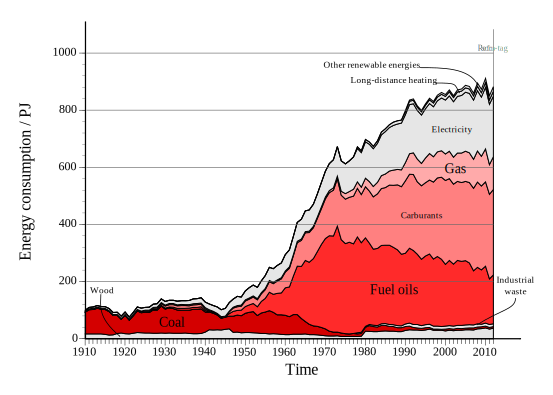
\includegraphics[height=10cm]{energy-consumption-switzerland-1910-2012-ofen-2012a-fig1p4}
  \caption[Final energy consumption in Switzerland]
  {Final energy consumption in Switzerland, based on the work of the
    \citet[Fig.\,1, p.\,4]{ofen-2012a}.}
  \label{fig:energy-consumption-ch-2012}
\end{figure}

\paragraph{The domestic sector represents about 30\% of the world
  final energy consumption} Investigating further this energy
consumption highlights that the worldwide domestic energy uses are
almost as high as the industry uses; they almost reach a third of the
global consumption and are mostly provided by fossil
fuels\index{energy consumption!fossil fuel consumption}. Indeed, the 3
big shares representing most of the global energy consumption are the
industry, with 33\% of the consumption, the domestic uses, with 29\%
(which are responsible of 21\% - 4.5 Gto of CO$_{2}$\index{carbon
  dioxide emissions} - of the carbon dioxide emissions), and the
transportation sector, with 26\%
\citep[p.\,17]{iea-2008a}\index{energy consumption}. Moreover, from
1973 to 2010, the ratio between the different fuels kept approximately
the same. The only significant exception concerns the transition from
coal to electricity \citep[p.\,28]{iea-2008a}, particularly motivated
by the development of the nuclear energy. During the period, natural
gas and oil consumption ratios also kept approximately
constant\index{energy consumption!fossil fuel consumption}. Global
energy use in the domestic sector increased between 1990 and 2005 by
19\%. Moreover, the domestic sector is the only major end-use sector
where the increase in energy consumption since 1990 has been greater
in OECD countries (+22\%) than in non-OECD countries (+18\%)
\citep[p.\,44]{iea-2008a}.


\paragraph{Space \& water heating represent about 70\% of the IEA19
  domestic sector energy consumption} In the IEA19
countries\footnotep{IEA19 is a set of 19 countries where extended
  energy data is available. Notably those 19 countries have domestic
  sector final energy consumption statistics available. The 19
  countries are Australia, Austria, Canada, Denmark, Finland, France,
  Germany, Ireland, Italy, Japan, Korea, Netherlands, New Zealand,
  Norway, Spain, Sweden, Switzerland, United Kingdom, United States of
  America.}, space heating remains the most important energy use,
responsible for 53\% of household final energy consumption, as
illustrated in \cref{fig:household-energy-consumption-2005}. This
share has decreased a bit (5\%) since 1990, but the energy saved has
been transferred to the appliance consumption. Space and water
heating, as illustrated in
\cref{fig:household-energy-consumption-2005}, make together an almost
stable consumption of about 70\% of the energy used in the domestic
sector over the last 25 years. Moreover, the share of the domestic
heating is considerably larger for the colder climates where space
heating demands higher temperature lifts, which are even higher for
the houses heated with conventional hydronic
systems\footnotep{Conventional hydronic systems may usually need
  water temperatures higher than 60\si{\degreeCelsius} while hydronic
  heating floor systems only need temperature up to
  35\si{\degreeCelsius}.}\index{energy consumption}.

\begin{figure}[htbp]
  \centering
  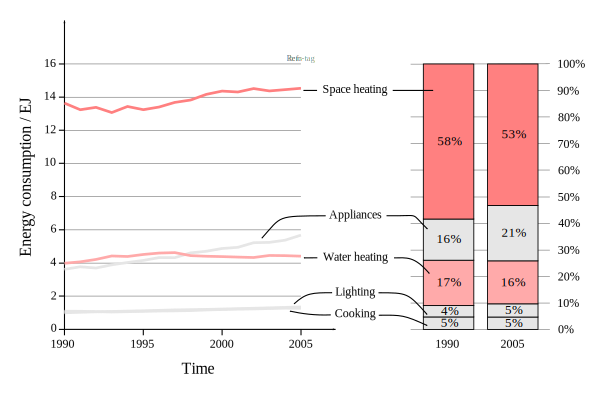
\includegraphics[height=10cm]{iea19-domestic-heating-iea-2008a-fig43p46}
  \caption[Final household energy consumption for the IEA19]
  {Final domestic sector energy consumption for the IEA19, based on
    the work of the \citet[Fig.\,4.3, p.\,46]{iea-2008a}.}
  \label{fig:household-energy-consumption-2005}
\end{figure}

\paragraph{Space \& water heating technologies for domestic uses}
Space and water heating is mostly performed around the world with fuel
consumption. The technologies involved are thermally-driven heat
pumps\index{heat pump!thermally-driven heat pump}, cogeneration,
fuel-cells, and of course, boilers. Direct electric heating is also
used, as is the use of electrically-driven heat pumps\index{heat
  pump!electrically-driven heat pump} (the latter still representing a
small share)\index{space \& water heating technologies}.

\paragraph{Heat pumps have a great potential to decrease the domestic
  energy consumption} Direct electric heating is a waste of energy, as
that electricity could be better used within an electrically-driven
heat pump\index{heat pump!electrically-driven heat pump}. Fuel-based
technologies play a role in an energy transition, especially the
fuel-cells, the thermally-driven heat pumps, and the cogeneration
technologies, but the human race needs in any case to dramatically
decrease its fossil fuel consumption\index{energy consumption!fossil
  fuel consumption} as soon as possible, in order to limit its carbon
dioxide emissions\index{carbon dioxide emissions}. Most of the climate
scientists in the world agreed through countless studies that those
emissions have a negative impact on the climate and the planet
ecosystems \citep{IPCC-2014a}\index{climate change}. Consequently, the
use of heat pumps\index{heat pump} to perform space and water heating
in the domestic sector appears as a key-technology for substantially
reducing both the energy consumption and the carbon dioxide
emissions. And it will be even more the case if the electricity
powering those heat pumps is produced in a sustainable way and from
renewable sources.


\paragraph{What is a heat pump?}
A heat pump\index{heat pump} is a device that extracts heat
energy\index{heat energy} from a source at low
temperature\index{temperature} and releases it at a higher temperature
\citep[based on def. p.\,607--608]{Borel-Favrat-2010a}. A heat pump is
based on a reversed Rankine cycle and can be made from different
variants (single-stage, two-stage, with internal heat exchangers,
etc...). This thesis work focuses on bithermal heating heat pump
cycles, also called thermopump
cycles. \citet[p.\,639--643]{Borel-Favrat-2010a} give an accurate and
detailed definition of this cycle. The basics to remember is that the
cycle happens in 4 main phases. First, low pressure, low temperature
gas is compressed during the compression phase\index{reversed Rankine
  cycle}, which releases this gas at high pressure, high
temperature. This gas is then condensed through a condensation
phase\index{reversed Rankine cycle}\index{heat exchanger!condenser},
which releases the refrigerant in a liquid state, at high pressure,
and lower, but still high temperature. Then follows an expansion
phase\index{reversed Rankine cycle}, where the high pressure, high
temperature refrigerant is expanded. It leaves in a two-phase state at
low pressure, low temperature. The last phase is the evaporation
phase\index{reversed Rankine cycle}\index{heat exchanger!evaporator}
which takes the two-phase refrigerant and evaporates it completely, in
order for it to enter the compression phase again. When the
refrigerant condenses in the condensation phase, it is at a higher
temperature than a house heating network. It releases heat
energy\index{heat energy}, usually to a water tank or to a house, in
domestic applications. When the refrigerant evaporates in the
evaporation phase, it is a temperature lower than the temperature of
the environment. It takes heat energy from it, as in domestic
applications, environment is usually the only source of heat energy,
also called cold source\footnotep{The hotter environment where the
  heat pump releases the heat energy is called the hot source.}. Heat
pumps can collect and release heat from and to different medias. Those
medias are fluids, in gaseous or liquid state. In domestic
applications, the medias used are usually water, brine\footnotep{Brine
  is a mixture of water and an antifreeze agent.}, or air. It exists
all the combinations of those medias in the domestic heat pump
world\index{heat pump!heat sources}: Air/Water heat pumps, Air/Air
heat pumps, Brine/Air heat pumps, Brine/Water heat pumps. Air/Air and
Air/Water heat pumps are the most common models, as they are cheaper
than the other versions, but they have also the lower performance
(the least efficient system being the Air/Air version). The Brine/Air
version is pretty uncommon and seldomly encountered. The Brine/Water
version is the most effective because the heat source is usually more
stable and at a higher temperature than the air energy source, and
also because the heat exchange is more efficient in Brine/Water heat
pumps, which decreases the losses in the heat exchangers\index{heat
  exchanger}.

\paragraph{About the refrigerants used  in heat pumps}

A refrigerant\index{refrigerant} is a fluid which condenses and
evaporates at pressure and temperature levels which are of interest
for the application. For domestic heat pumps applications, many fluids
can be used as refrigerants. The latter can be natural fluids or
synthetic fluids. They can be used pure, or blended together in
specific proportions, the blend getting convenient characteristics for
the application. The choice of a refrigerant for a thermodynamic cycle
is a critical one, as there are technical characteristics to take into
account, but also legislative constraints, related to regulations. A
refrigerant could have an impact on the atmospheric ozone layer
depletion, if released. Most of the forbidden refrigerants had an
\ODP{}. Nowadays refrigerants have no ozone
depletion potential. Refrigerants could also have a negative impact on
the greenhouse effect, if released in the atmosphere. Most of the
refrigerants have a global warming potential. The trend worldwide is
to use refrigerants with a global warming potential as low as
possible. Nowadays, the trend is to use more and more natural fluids
as refrigerants, as they have usually lower global warming potentials
than synthetic refrigerants (and consequently lower legal constraints
related to regulations). The issue with natural fluids is mainly
that, often, they are either toxic, flammable, or explosive.

\section{Better domestic heat pumps can help}
\label{sec:better-hp}

Better domestic heat pumps can help to slow down the energy
consumption. Better domestic heat pumps are needed. The better
domestic heat pumps should be:

\begin{description}
\item[More efficient] \citet{Zehnder-2004a} and
  \citet{barbouchi-2007a} demonstrate in their work the importance of
  the exergy losses in the compression phase.  \citet[Fig.\,I.2
  p.\,206]{barbouchi-2007a} demonstrates with his simulation work an
  exergy loss of 49\% for a two-stage compression phase, and of 57\%
  for a single-stage compression phase. The heat pump thermodynamic
  cycle being considered in this study was a A5/W48
  cycle. \citet[p.\,227]{Zehnder-2004a} demonstrates with his
  simulation work an exergy loss of 60.3\% for a single compression
  phase, and of 50.5\% for a twin-stage compression phase. The heat
  pump thermodynamic cycle being considered in this study was a
  A-12/W60 cycle. As a consequence, in order to significantly improve
  the performance of the domestic heat pumps, the compression phase
  efficiency has to be improved as much as possible. Therefore, to
  improve the domestic heat pump performance, a technological gap on
  the compression device is necessary. This is the motivation for the
  radial compressor development performed by \citet{schiffmann-2008a}.
\item[More compact] More compact heat pumps opens the way to their use
  in places where they could not be used before. If they get compact
  enough, they can be used in flats, replacing boilers, for
  instance. They could also be used for waste water heat recovery.
\item[Less material] A significant share of the metals used in human
  machinery becomes harder to extract from the Earth crust, as they
  rarefy. It increases the cost of production of the machinery and
  decreases their sustainability. Consequently, the less raw material
  needed, the better.
\item[Less noise] In order to be used in flat or small homes, the heat
  pumps need to be as silent as possible.
\item[Decreased impacts of the refrigerant] The refrigerant used in
  the heat pumps should have a low impact on the environment or the
  climate, as they are elements to be preserved for our own sake. In
  the same spirit, the refrigerant charge should be kept as low as
  possible, in order to decrease the impact of leakages and the
  security risks.
\end{description}

\section{Scope of this thesis work}
\label{sec:intro-thesis-scope}

This thesis work focuses on the experimental investigation of two
electrical domestic heat pump prototypes equipped with a twin-stage
oil-free radial compression unit. The two prototypes tested have been
designed, built, and tested during this thesis work. They are the
first worldwide working prototype of domestic heat pumps powered with
radial oil-free compressors. \Cref{chap:intro} is the introduction
motivating the need for better domestic heat pumps are
needed. \Cref{chap:sota} is a literature review stating some paths of
improvement for the domestic heat pumps. \Cref{chap:methodo} presents
the thesis to validate and the methodology
applied. \Cref{chap:awp,chap:bwp} present the prototypes, their test
results, the issues encountered, and the observations
made. \Cref{chap:cp-intg} presents additional ways of improvement of
the two prototypes and highlights good practices regarding oil-free
heat pump design. \Cref{chap:conclusion} concludes this thesis work by
validating the thesis proposed in \cref{chap:methodo}. The originality
of this thesis work articulates around of the following points:

\begin{enumerate}
\item The two prototypes that have been designed, built, and tested
  are the two first low power heat pumps powered by low power oil-free
  radial compressors successfully tested worldwide. This is the first
  time that such achievement is reached and documented. The two prototypes allowed to gain a lot of experience about the
  issues related to oil-free systems and knowledge about good
  practices for the design of such devices.
\item An original design of economizer has been developed for the
  \AWP{}. This economizer is equipped with an efficient liquid/gas
  separator and combines directly with the volute of the compression
  unit, already starting an integration process of the heat pump parts
  together.
\item Building onto the experience gained during the experiments,
  original designs are offered for advanced concepts of bypass systems
  and first stage separator. An original integrated design concept of
  compression unit module including the first stage separator and the
  economizer is also offered.
\item The modeling approach offered in this work to analyse the experimental data transposes a software
  modeling tool to the energy analysis domain. The use of this tool
  makes the modeling easier by systematizing the generation of the set
  of equations, making the modeling steps easier and more reliable.
\end{enumerate}


\FloatBarrier
\bibliographystyle{plainnat}
\bibliography{main}
\label{sec:references-intro}

\section*{Credits}
\label{sec:intro-credits}
\addcontentsline{toc}{section}{Credits}
\phantomsection

\begin{description}
\item[\figref{fig:energy-consumption-ch-2012}] \ccbyjb{2013}. This
  figure is based on an original figure from the \citet[Fig. 1,
  p. 4]{ofen-2012a}.
\item[\figref{fig:household-energy-consumption-2005}]
    \ccbyjb{2013}. This figure is based on an original figure from the
    \citet[Fig. 4.3, p. 46]{iea-2008a}.
\end{description}


%% State of the technique
%% How to make better domestic heat pumps?
\chapter{State of the art}
\label{chap:sota}
\resetallacronyms

\begin{shaded}
  This chapter exposes what are the different ways to improve heat
  pump systems through a review of the available
  literature. Multistage, oil-free, and variable-speed technologies
  show promising perspectives in the heat pumps application fields and
  allow to make more efficient, more compact, more silent heat pump
  circuits built with less raw material and using a lower refrigerant
  charge.
\end{shaded}

As explained in \cref{sec:intro-slow-energy}, there are different
types of heat pumps. The interest in this chapter is focused on
electrically-driven vapor compression domestic heat pumps.

\section{Types of refrigerant compressors}

\subsection{Dynamic versus volumetric}
\label{sec:sota-dyn-vs-vol}

Refrigeration systems equipped with dynamic compressors are expected
to develop better seasonal performance than those equipped with
volumetric compressors. Indeed, soon after the scroll compressor
technology release, \citet{Purvis-1987a} described scroll-based heat
pump systems capacity response to the residential heating demand. Heat
pumps using volumetric compression devices, like scroll compressors
(the other types of volumetric compressors are even more concerned by
this trend according to \citet{ASHRAE-HVACeq-2008a-Compressor}), are
characterized by a decrease of their capacity as the outside
temperature decreases, while the residential demand evolves
inversely. This behavior explains why the heat pumps used for space or
water heating in residences must be designed to provide the heating
demand for the lowest expected outside temperature in the geographic
area. It implies that the heat pump, whose function would be to heat
the houses without any auxiliary device (like a boiler or an electric
resistor to compensate for the heat pump, or replace it totally when
outside temperature becomes too low), will be significantly
over-sized, during most of the heating period. As explained by
\citet[p.\,1922]{Schiffmann-Favrat-2009a}, variable-speed dynamic
compressors do not behave this way and stick with the residence demand
curve. They are also expected to develop better isentropic
efficiencies\footnotep{The isentropic efficiency of a compressor is
  defined in \cpref{sec:methodo-indicators}.}. Consequently using
dynamic compressors in domestic heat pump circuits would result in a
much better energy use and, potentially, in a maximization of the
efficiency, since it becomes possible to choose the exact compressor
speed which maximizes the compressor efficiency for the given mass
flow rate and pressure ratio needed. Additionally, the compression
unit would not need to be over-sized which would result in a more
rational use of raw materials and result in a smaller compression
unit, which also increases the compactness potential.

\subsection{Volumetric compressors used in domestic
  heat pumps}
\label{sec:sota-vol-cp}

The main volumetric compressor (also called positive-displacement
compressor) technologies used in refrigeration circuits are:

\begin{description}
\item[Reciprocating compressors:] Piston compressors are also known as
  reciprocating compressors. Linear stroke compressors are also
  reciprocating compressors. Historically, that compression technology
  is the first one to have powered vapor compression domestic heat
  pumps, from after somewhere between the two World Wars
  \citep[p.\,23]{zogg-2008a} to the 1980s, when the scroll compressors
  have been introduced. From that point in time, reciprocating
  compressors started to be replaced by scroll compressors in the
  domestic heat pump application. Scroll compressors were cheaper,
  more reliable, needed less maintenance, and were less noisy. In the
  1990s, most of the vapor compression domestic heat pumps are
  equipped with scroll compressors, instead of reciprocating
  compressors. Reciprocating compressors had to be lubricated to work
  properly and to not fail. With the increase of the accuracy of the
  manufacturing methods and the development of new design, linear
  stroke compressors without lubrication start to be produced. They
  target first the domestic refrigerators application, but are also
  used in some other applications, like in the study made by
  \citet{Marcinichen-Michel-2014a}. For instance,
  \citet{Marcinichen-Michel-2014a} used an oil-free 125W
  \citep[Tab.\,1, p.\,183]{Marcinichen-Michel-2014a} linear stroke
  mini-compressor capable of modulating its volumetric displacement on
  a share of the stroke \citep[p.\,183]{Marcinichen-Michel-2014a} and,
  an oil-free magnetically driven liquid gear pump to perform
  two-phase chip cooling. The compressor power of the compressor
  selected in the paper from \citet{Marcinichen-Michel-2014a} would
  not fit for domestic heating applications as its power is very
  low. Generally speaking, totally oil-free linear stroke compressors
  are limited in power range and are usually dedicated to household
  refrigerators applications, where they greatly contributed to
  increase the system performance
  \citep{Bansal-Abdelaziz-2011a}. However,
  \citet[p.\,186]{Marcinichen-Michel-2014a} consider the efficiency of
  such a compressor still low compared with conventional domestic
  heating heat pump compressors.
\item[Scroll compressors:]\label{sec:sota-scroll}A scroll compressor
  is an involute profile, mounted on a rotor, that rolls onto an other
  involute profile, which is usually fixed, and that is sightly
  offset. The involutes are drawn in a way that reduces the volume of
  the compression space further and further during the rotation of the
  shaft. The geometry of the scroll compressor has been invented by
  \citet{creux-1905a} at the beginning of the 20\th{} and did not
  really changed ever since. The involute profile is described
  mathematically by two Archimedean spirals with the same generating
  circle, and separated by a constant offset. They also can be
  generated from hybrid curves. The scroll compressor has not been
  commercialized until the early 1980s, as it had to wait for the
  development of effective high-accuracy, high volumes manufacturing
  techniques to be developed because of the complexity of the shapes
  involved \citep[p.\,16]{zogg-2008a}. Between the 1980s and 1995, the
  performance of the scroll compressors has been optimized and
  increased, then, after the introduction of the last generation of
  scroll compressors between 1992 and 1995, the increase of
  performance stopped. The data collected by
  \citet{Eschmann-2009a}\footnotep{\citet{Eschmann-2009a} performed a
    monitoring study on Brine/Water and Air/Water domestic heat pumps
    whose performance had been measured at the Swiss heat pump
    certification center between 1992 and 2007.} and summarized in his
  report of 2008 highlights the stagnation of the heat pump
  performance since the introduction of this last generation of scroll
  compressors. Nowadays development of this technology takes new
  paths, like the one explored by \citet{Iglesias-favrat-2014a}. They
  presented a prototype of oil-free scroll air compressor with two
  mobile involutes working in synchronized co-rotation one relative to
  another. The prototype can also work as a turbine, as the compressor
  is reversible. This concept could theoretically be applied with
  refrigeration compression, even if the technical challenges are
  significant. For instance, injection of liquid refrigerant during
  the compression in the volutes could also be
  done. \citet{Zehnder-2004a} has documented this kind of humid vapor
  injection in his work \citep{zehnder-favrat-2010a}, but in his case,
  one of the involutes was fixed, as he was working with an orbital
  scroll, which was making the process easier. Using co-rotative
  scrolls greatly limit the efforts on the bearings and results in a
  balanced setting \citep[Fig.\,2 p.\,567]{Iglesias-favrat-2014a},
  which makes it an interesting concept for oil-free
  applications. Nonetheless, it seems that the development of the
  scroll compressors reaches technological limits and will not
  increase its performance significantly, with the current technology
  state.
\item[Rotary vane compressors:]Rotary vane compressors are made of a
  rotor with blades inserted in radial slots in the rotor. When the
  rotor turns, the blades slide in and out of the slots, keeping
  contact with the outer wall of the compressor housing. As the rotor
  is not at the center of the housing, the gas is being compressed by
  a reduction of the volume between the blades. Those compression
  devices are being introduced recently in the domestic heat pump
  sector as a second compression stage on top of a scroll compressor
  \citep{Kondo-Kimata-2010a,Mitsubishi-2011a,Sato-Kobayashi-2012a}. A
  rotary vane compressor can be multistage and is a lot quieter than
  the reciprocating technology, at equivalent power.
\end{description}

\subsection{Dynamic compressors used in domestic
  heat pumps}
\label{sec:sota-dyn-cp}

There is no dynamic compressor technology used in the heat pump
domestic sector currently, but one is coming with the developments
performed since the beginning of the 21\th century, notably with the
work of \citet{schiffmann-2008a}.

\paragraph{Radial compressors}

The first radial compressors were manufactured at the beginning of the
$20^{\text{th}}$ century. They were originally developed by steam
turbine manufacturers and were widely used for ventilation purposes in
deep mining. At that time, the possibilities of producing an impeller
were rather limited by the manufacturing technology available. Decades
later, the manufacturing technologies had evolved and started to allow
the manufacturing of highly efficient radial compressors. Carrier has
been the first to work seriously on radial compressors from 1911 for
refrigeration applications (at the time, it was for air
conditioning). In about 1919, he first tried a German radial
compressor with di-chloroethylene, and then a compressor made by
Eastman Kodak in the United States with dichloromethane
\citep[p.\,16]{zogg-2008a}. They have been used in industrial
refrigeration circuits from the beginning of the 20\th{} century to
nowadays, and they now can be used in domestic heat pump applications
due to the recent development of the manufacturing processes and the
development of small scale gas bearings sets specially designed for
this application, with an integrated-design approach
\citep{schiffmann-2008a}.

\subsection{About the compression units used in this thesis work}
\label{sec:sota-jurg-cp}

\citet{Schiffmann-Favrat-2009a} presented in 2009 really encouraging
experimental results with the testing of a single-stage compression
unit. They also presented promising preliminary simulation results for
a twin-stage heat pump based on the radial compressor unit that
\citet{schiffmann-2008a} was developing. That compression unit, and
its successors, the twin-stage compression units used in this thesis
work, are at the cutting edge of the technique and the technology
reachable nowadays, as shown in \cref{fig:zwyssig}. Those compression
units are several times lighter and smaller than their equivalent in
the scroll technology, as illustrated in
\cref{fig:cp-unit-volume-comparison} and are expected to demonstrate
the greatest potential in many processes where gas compression is
needed. A similar design has been used by
\citet{demierre-wegele-2014a} with a compressor-turbine unit, using a
radial compressor and a radial turbine, mounted at the two sides of a
same shaft\footnotep{Details about this specific design can be found
  in the thesis work of \citet{demierre-2012a}.}. The twin-stage
compression units powering the \AWP{} and the \BWP{} have been
developed between 2002, when the feasibility study of the twin-stage
unit has been presented by \citet{schiffmann-godat-2002a}, and 2012,
when the first compression unit prototype has been able to power a
heat pump cycle in an experimental setup. The results of those first
experiments are presented in \cpref{chap:awp}.

\begin{figure}[htbp]
  \centering
  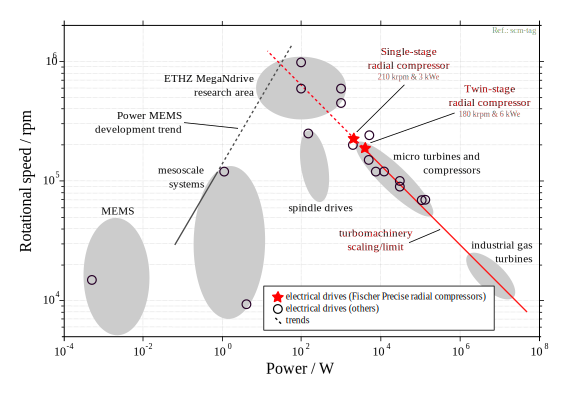
\includegraphics[width=\textwidth]{zwyssig-round-2009a-fig1p565-augmented}
  \caption[Trends for high speed electrical drives and
  turbomachineries.]
  {Emerging application areas and trends for high speed electrical
    drives and turbomachineries, based on the work of \citet[Fig.\,1,
    p.\,565]{zwyssig-round-2009a}.}
  \label{fig:zwyssig}
\end{figure}

\begin{figure}[htbp]
  \centering \subfloat[Compression unit aside a 1.5-liter water bottle]
  {\label{fig:cp-unit-1L}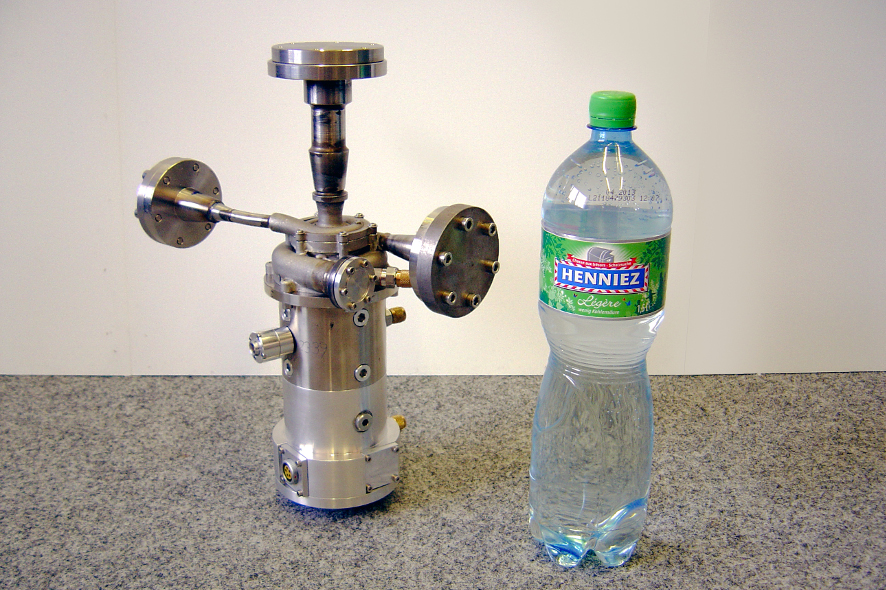
\includegraphics[width=0.45\linewidth]{20121219T094101-00066bis}}
  \hspace{1em} \subfloat[The compression unit is equivalent to 2 scroll
  compressors]
  {\label{fig:cp-unit-scrolls}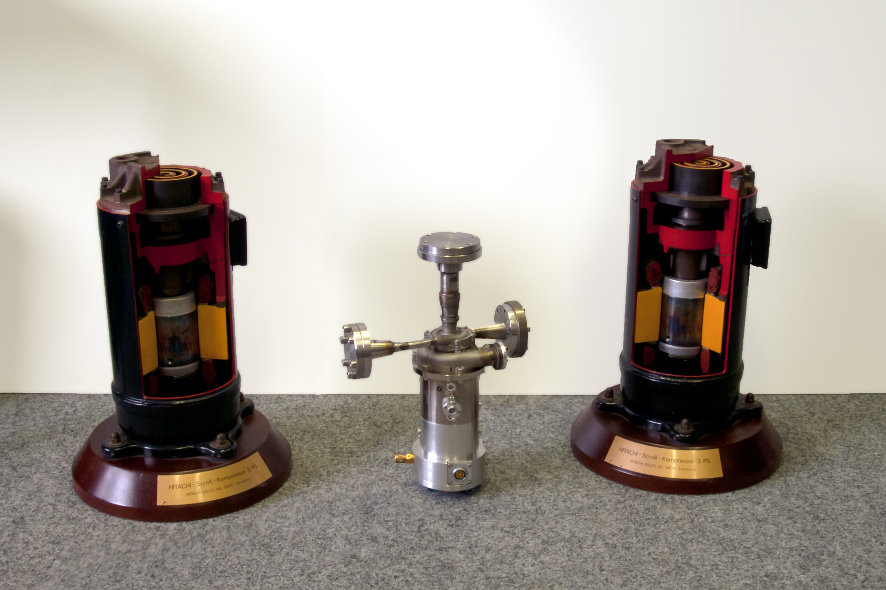
\includegraphics[width=0.45\linewidth]{20121218T525614-0049+0050}}
  \caption[Volume of the twin-stage compression unit]{The volume and
    the weight of the twin-stage compression unit are several times
    lower than a single-stage scroll compressor. The 6 kW twin-stage
    compression unit is roughly equivalent to 2 single-stage 3 kW
    scroll compressors.}
  \label{fig:cp-unit-volume-comparison}
\end{figure}

\section{Noise reduction in refrigeration circuits}

As very accurately balanced and high rotation speed devices, the
compression unit developed by \citet{schiffmann-2008a} and its
successors produce no vibrations and can be made very silent. In
opposition to typical scroll compressors that produce a lot of
vibrations and noise (about 65 dBA, on average, according to
\citet{ARI-270-94} compliant measurements, at the nominal compressor
speed of 50 Hz \citep[Fig.\,43,
p.\,37.26]{ASHRAE-HVACeq-2008a-Compressor}), widely spread on the
audible sound spectrum. This implies that this noise is difficult to
insulate, on the contrary to the radial compression units, which
produce high frequency noises due to their high rotational speed and
the gas bearings technology (no friction). As those high frequencies
are easy to staunch with basic sound insulation, radial compression
unit rotating on gas bearings can be made very silent. Furthermore,
regular Air/Water domestic heat pumps available in th
\citet{Eurovent-2010a} database release between 53 and 83 dBA (with
fans), according to ISO\,9614 \citep{EN-ISO-9614-1} ans ISO\,3744
\citep{ISO-3744-2010a} compliant measurements. Consequently,
compressor noise constitutes a significant part of the heat pump
noise. Thus, switching to radial compression unit rotating on gas
bearings and to silent fans open the way to very quiet heating
machinery.

\section{Variable-speed in refrigeration circuits}

Variable-speed capacity control has been proven to increase heat pump
efficiency \citep{Karlsson-2003a,Karlsson-Fahlen-2008a}. There are
different ways to obtain this capacity control.

Heat pump capacity control is performed by reducing the compressor
capacity.  In domestic heat pumps, most of the compressor used are
scroll compressors.  Those device are currently using one of the three
technologies detailed below to control their capacity.

\paragraph{Variable displacement based capacity control:}

This mechanism is dedicated to scroll compressors and consists in
ports incorporated in the fixed scroll. The control consists in the
connection or not of the compression chamber to the suction side by
respectively closing or opening the ports. Then, when the
ports are all closed, the compressor runs at its full
capacity. To provide only a share of the full capacity, some holes are
open. The number of different capacities and extent of the capacity
reduction available is governed by the locations of the ports.

\paragraph{Pulse Width Modulation based capacity control:}

This mechanism is also dedicated only to scroll compressors and
consists in a device that modulates the axial pressure that maintains
sealing contact between the scroll tips and its base. The control is
done by cycling the loading and unloading of the fixed scroll without
changing the motor speed.  The cycle is controlled by an electrical
devices which adapt the loading and unloading phases to make the
compressor deliver the exact capacity required.

\paragraph{Variable speed based capacity control:}

The compressor is driven by an inverter to convert the 50 Hz
fixed-frequency alternative current coming from the power network to
an adjustable voltage and frequency signal. This signal is then used
to control the speed of the motor, which is correlated with the mass
flow rate of the refrigerant through an equation or a compression
map. This capacity control strategy is used on some scroll compressors
and is the solution selected for the control of the radial compression
units used in this thesis work.

\section{Multistage refrigeration circuits}
\label{sec:sota-multistage}

Two-stage compression cycles has been proved to reach higher
performance than single-stage cycles in various studies
\citep{Favrat-Courtin-1997a,Zehnder-2004a}. Moreover, this statement
is particularly true for high temperature differences between the hot
source and the cold source. \citet{Zehnder-2004a} presented several
twin-stage heat-pump configurations and tested some of them
\citep{Zehnder-Favrat-1998a,Zehnder-Perevozchikow-2002a}. The most promising cycles were the
following:

\begin{description}
\item[Solution \#1:] Addition of a separate single-stage heat-pump
  cycle to a main single-stage heat-pump cycle. The main cycle is
  dedicated to the heating of the house while the additional cycle
  uses the subcooled liquid at the outlet of the main condenser as a
  cold source to produce tap water.
\item[Solution \#2:] Superposition of two single-stage heat-pump cycles
  coupled with a shared heat exchanger acting as the condenser for the
  bottoming cycle and an evaporator for the topping cycle.
\item[Solution \#3:] A single-stage cycle using a single-stage
  compressor with intermediate vapor-injection.
  \begin{description}
  \item[\#3.1:] The vapor injected during the compression process is
    produced by the expansion of subcooled liquid removed at the
    outlet of the condenser. Before being injected, the wet vapor is
    heated up by going though an intermediate heat exchanger,
    exchanging heat between the main subcooled liquid line and the wet
    vapor previously expanded
    \citep{Zehnder-Favrat-2002a,Beeton-Pham-2003a}. When the vapor
    exchanges heat in the intermediate heat exchanger, its vapor
    quality increases. Often, the vapor injected in the compressor is
    just saturated. Wet vapor injection is only needed if the outlet
    temperatures are getting too high.
  \item[\#3.2:] The subcooled liquid coming from the condenser is
    expanded to an intermediate pressure and enters a flash tank where
    vapor and liquid are separated. Liquid is expanded and enters the
    evaporator while vapor is injected in the compressor, during the
    compression process.
  \end{description}
\item[Solution \#4:] A twin-stage heat-pump using a twin-stage
  compressor and an intermediate heat exchanger or a flash tank in
  order to inject vapor between the two compression stages, as in the
  two versions of the above solution.
\end{description}

\citet{Schiffmann-Favrat-2005a} have analyzed those different concepts
in order to design a domestic, high temperature lift, air-water heat
pump. They sum up those concepts in a later article
\citep{Schiffmann-Favrat-2009a} and conclude notably that the solution
\#4, with a flash tank acting as an economizer, is the most
interesting one, when taking in account the radial compressors
characteristics and limitations. Moreover, they pointed out that this
solution is an elegant one in terms of number of components and
control, and a promising one in term of \COP{}
\citep{schiffmann-2008a,Favrat-Courtin-1997a}. They also indicate
that, with this cycle configuration, inverting the cycle in order to
defrost the evaporator, could allow to use the economizer as an
internal energy source. Since the final goal is the development of a
twin-stage oil-free air-water heat-pump using a twin-stage radial
compressor rotating on gas bearings, the configuration \#4 is
favored. This configuration is referred as a twin-stage compression
cycle with flash cooling, as it has been named by the ASHRAE
\citep[Fig.\,49, p.\,37.29]{ASHRAE-HVACeq-2008a-Compressor}.

\section{Lubrication in refrigeration circuits}

\citet{YoubiIdrissi-Bonjour-2008a} highlight that, currently, almost
every refrigeration vapor compression systems need a lubrication
agent, which is generally a mineral or synthetic lubricant oil
depending on the refrigerant used in the system. Oil functions are (1)
to protect the mechanical moving elements against the wear with a thin
lubricant film, (2) to act as a sealing element, (3) to limit the
noise made by the mechanisms, (4) to help the evacuation of chemical
impurities or deposits which may be present in the circuits, and (5)
to act as a heat transfer medium for cooling the compressor, in many
systems. Those favorable or vital functions clearly assert that oil in
refrigeration compression systems is generally compulsory and
useful. However, that oil brings also severe drawbacks to the
refrigeration circuits. Most of the time, it reduces the heat transfer
coefficient in heat exchangers, it changes the flow configurations, it
increases the pressure drops, and it modifies the thermodynamic
equilibrium and the thermodynamic properties of the refrigerant
\citep{YoubiIdrissi-Bonjour-2008a}.

\subsubsection{Migration of the oil inside the heat pump loops}
\label{sec:migration}

\citet{Zehnder-2004a} studied the migration of the oil into a
twin-stage heat pump loop. He concluded that the oil is migrating from
the topping stage compressor to the bottoming stage compressor and
could not identify a stable situation where this statement was
false. The topping compressor, a scroll compressor, without lubricant
oil recovery circuit, dries and is doomed to failure. Moreover,
\citet{Navarro-Corberan-2005a} studied the oil circulation ratio and
its return to the compressor with R290/\POE{} and R407C/\POE{}, on a
reciprocating compressor installation and compared their results with
mineral oil experiments. They found that the oil would return easier
to the compressor if it is a \POE{} than if it is a mineral oil. They
concluded also that there is no behavior difference, from the oil
point of view, with R290 or R407C but this conclusion is deduced from
a single-stage heat pump loop. \citet{Winandy-Cuevas-2003a} has
studied the oil level in two scroll compressor in parallel, in a
refrigeration installation. They demonstrated that the oil was not
returning equally to the two compressors, especially when working
under part load. They also linked the two compressor housings with a
straight pipe, welded at the normal height of the oil-levels, allowing
an oil-level adjustment between the two compressors and concluded the
oil migration phenomenon has to be taken seriously, even more
seriously when running under part-load. Unfortunately, in twin-stage
heat pumps based on 2 scroll compressors, since the pressure level is
not the same for the two compression devices, in opposition to the two
scroll compressors in parallel presented by
\citet{Winandy-Cuevas-2003a}, this solution is not applicable. The
direct consequence of those studies is that it should be a lot easier
to make multistage heat pump devices without having to consider the
return of the lubricant agent to the compressors. Those heat pumps are
likely to be more reliable also, as they won't fail because of
lubrication issues. Additionally, using oil-free circuits allows to
get free from the design rules of circuits with oil. For instance, the
pipe diameters can be increased in the suction lines in order to
decrease the pressure drop on the vapor line, generating exergy
losses\footnotep{Exergy and exergy efficiency are defined in
  \cpref{sec:methodo-indicators}.}. Those pipes diameters are limited
in the circuits with oil because the oil has to be recovered in the
compressor housing \citep{kesim-ileri-2000a,Guo-Shen-2011a}. This
problem is even more acute with variable flow capacities linked to
variable speed compressors.

\subsection{Impact of the lubricant on the expansion process}
\label{sec:oil-dv}

\subsubsection{Electronic expansion valves}

\citet{Liang-Zhijiu-2009a} have established models of electronic
expansion valves for R22, R407C and R410a based on Bernoulli equation
giving accurate results. The models they propose differ from some
conventional models using the two-phase outlet pressure and corrected
flow coefficient since they consider metastable phenomenona caused by
rapid depressurization and employ the throat pressure of the
electronic expansion valves and the single-phase incompressible flow
coefficient. \citet{Park-Kim-2007a} have used a different approach
using a model with a set of parameters and variables including the
valve geometry, its inlet and outlet conditions, and the refrigerant
thermodynamics properties to describe the valves behavior. Both of
those studies are dealing with pure refrigerant or neglect the
presence of oil. For now, influence of oil seems not to be documented
or considered as negligible, but it could be a problem with oil-free
circuits.

\subsubsection{Capillary tubes}

There are two groups of studies dealing with the effect of oil in the
capillary tubes. The first deals with oil-rich mixtures, with
typically more than 5\% in weight, while the second treats the oil as
a contaminant, present in quantities lower than 5\% in weight. The
studies where important quantities of oil are mixed with the
refrigerant are quite seldom but are interesting to understand and
interpret the foaming phenomenon occurring in compressors, as the oil
concentration is the highest in those devices. For instance,
\citet{Poiate-Gasche-2006a} studied the foaming phenomenon inside
small tubes. The second case is more usual and several studies have
been published. Most of them aim to improve the knowledge available on
the phenomena which occur in capillary tubes, like two-phase flow
pressure drop or metastable flow\footnotep{A metastable flow remains
  liquid over a distance longer than the one predicted by conventional
  pressure drop models.}. \citet{Motta-Braga-2002a} performed visual
experiments to determine the position of the vaporisation point of a
R404a-oil mixture inside a capillary tube and quantified the effect of
a given percentage of oil on the capillary tube behavior. Some of the
studies observed a reduction in the mass flow rate with an increase of
the oil concentration \citep{Motta-Parise-2001a,Fukuta-Ogi-2003a}.

\subsection{Impact of the lubricant on the evaporation
  process}
\label{sec:oil-ev}

The evaporation process is known for decades to be the more sensitive
process of the heat pump cycle regarding the presence of compressor
lubrication oil in the refrigerant. \citet{McMullan-Murphy-1992a} have
shown that the viscosity of the lubrication oil has a negative effect
on the evaporator performance for a fully miscible oil-refrigerant
mixture. For shell-and-tubes evaporators, they concluded that the
addition of oil produces a change in the refrigerant two-phase flow
regimes and a decrease of the overall evaporator performance. Previous
studies
\citep{McMullan-Hughes-1988b,McMullan-Hughes-1988a,Hughes-Morgan-1984a,Hughes-Morgan-1982a,Hughes-Sutcliffe-1980a,Hughes-Morgan-1984b},
observed the lubricant oil influence on the heat pump performance and
concluded that the presence of oil in the evaporator was responsible
of a significant decrease of performance. They also concluded that the
accumulation of oil at the end of the evaporator (refrigerant
vaporizes, oil just flows), has a significant influence on the
decrease of the heat transfer coefficient which is observed. They have
estimated that, in principle, an evaporator working with no oil at all
would allow an increase of the whole evaporator heat exchange
coefficient by about 40\%
\citep[p.\,123]{McMullan-Morgan-1983a}. Indeed, the more refrigerant
evaporates, the more the remaining liquid refrigerant is charged in
oil, and the more it is difficult for it to evaporate. The potential
improvement of 40\% is certainly quite optimistic, but it remains that
improvements of the heat exchange coefficient are observed with the
decrease of the oil mass faction. If oil can not be removed, from an
heat exchange point of view, \citet{McMullan-Morgan-1983a} added that,
for low amounts of oil in the refrigerant, a low viscosity oil leads
to better results, while for bigger amount of oil in the refrigerant,
high viscosity oil would be the better choice. They also observed that
the presence of oil increases the pressure drop into the
evaporator. \citet{Spindler-Hahne-2009a} have studied the influence of
oil on nucleate pool boiling heat transfer with enhanced surface
tubes. They concluded that, except under very specific conditions, oil
always decreases the heat transfer coefficient \citep[Fig.\,19
p.\,990]{Spindler-Hahne-2009a} and \citep{Moller-1998a}. The more oil
there is, the less efficient the evaporation is.
\citet{Nidegger-Thome-1997a} and \citet{Zurcher-Favrat-1998a} have
studied the intube flow boiling of R-407C and R-407C-oil mixtures
\citep{Zurcher-Favrat-1998a,Zurcher-Favrat-1998b}, and the R134a and
R134a-oil mixtures \citep{Zurcher-Favrat-1997a,Nidegger-Thome-1997a},
both on plain tubes and microfins tubes, and confirmed the
observations of \citet{McMullan-Morgan-1983a}: with increasing oil
concentration, the heat transfer coefficient drops. Some authors, like
\citet{Cawte-Poland-1996a}, observed, in the contrary, an increase of
the heat transfer if the oil concentration reaches a certain range (2
to 10\% in the case of the study published by
\citet{Cawte-Poland-1996a}). \citet{BandarraFilho-Thome-2009a}
reviewed a great number of papers involving refrigerant–oil mixtures
that can be found for different test conditions and found that they
often present conflicting results, unfortunately. Even so, it is still
possible to affirm that some thermodynamic properties of
refrigerant/oil mixtures, such as density, viscosity, surface tension
and miscibility, can modify, specifically, the heat transfer and
pressure drop, and thus affect directly the \COP{} of the system
\citep[p.\,186]{BandarraFilho-Thome-2009a}. \citet{Cawte-1992a}
performed similar heat transfer studies on condensation processes with
refrigerant/oil mixtures and observed a big non-linear decrease of the
heat coefficient with the increase of the oil concentration. However,
he concludes that this change of heat transfer coefficient has little
impact on the whole heat pump performance. Of course, it is important
to consider that most of those studies have been made on plain tubes,
or conventional surfaces.

\subsection{Oil-free heat exchange technologies}
\label{sec:sota-oilfree-hx}

Using oil-free compression devices opens the way to the use of
existing or to-develop heat exchangers, which would be more efficient
or become usable with oil-free compression technologies. Those heat
exchangers include micro-channels heat exchangers, direct ground
evaporators, and heat exchangers using enhanced surfaces, like
enhanced tubes-based heat exchangers
\citep{Ribatski-Jacobi-2005a,Habert-2009a,vanrooyen-2011a} or enhanced
plate-based heat exchangers \citep{Furberg-2006a}, which would result
in a reduction of the heat exchange surfaces, and consequently, in a
reduction of the pressure drops inside the circuits and of the whole
heat pump size. Furthermore, some of those heat exchange technologies
open the way to heat exchangers with reduced temperature pinches
between the refrigerant and the heat source and would contribute to
decrease the exergy losses coming from the heat
exchanges. \citet{Furberg-2006a} and \citet{Li-2008a} develop plates
heat exchangers with enhanced surfaces with micro patterns
\citep{Furberg-Muhammed-2009a}. Enhanced surfaces with micro-patterns
are filled with oil, if used with refrigerant-oil mixtures
\citep[Fig.\,10\,\&\,11 p.\,985--986]{Spindler-Hahne-2009a} and
thereby become less efficient. Consequently, the enhanced plate heat
exchangers developed by \citet{Furberg-Muhammed-2009a} mainly target
oil-free applications. Oil free heat exchange technologies are in
heavy development since the last 20 years \citep[Fig.\,1
p.\,186]{BandarraFilho-Thome-2009a}, as new market applications
emerge. Their application in oil-free compact domestic heat pumps
promises to increase even further the potential of the oil-free
compression technologies.

\subsection{Impact of the lubricant oil on the
  compression process}
\label{sec:oil-cp}

One of the main effect of oil in the compression process is the
foaming phenomenon, which is due to the interactions between the oil
and the refrigerant induced by the blade rotation or the vapor
blow. The foaming phenomenon has been studied in a hermetic casing
simulating a hermetic rotary compressor by
\citet{Yanagisawa-Fukuta-1991a}. They observed that the foaming
increases and become massive for high compressor blade speed combined
with a high mass flow rate. Another effect of the oil on the
compression process is the modification of the compressor
performance. Indeed, because of the solubility of the oil into the
refrigerants\footnotep{The solubility of the oil into the refrigerant
  is proved to increase with pressure
  \citep{Wahlstrom-Vamling-1997a}.}, the refrigerant-oil mixture
enthalpy may be substancially different from the pure refrigerant
enthalpy \citep[Fig.\,2--4,
p.\,288--289]{YoubiIdrissi-Meunier-2003a}. As a consequence, the
energy balance performed on the compressor may be false and, as shown
with the \citet[Fig.\,2--4, p.\,288--289]{YoubiIdrissi-Meunier-2003a}
diagrams, it leads to wrong estimations of the refrigerant mass flow
rate. Indeed, considering pure refrigerant instead of the real
oil-mixture that really flows out of the compressors leads to make a
mistake on the enthalpies at the inlet and the outlet of the
compressors, which is reflected on the energy balance, and finally on
the mass flow rates. As some refrigerant remains dissolved in the oil,
some liquid desorbs from the oil during the compression process,
inducing a wet compression process. This phenomenon may considerably
affect the compressor isentropic efficiency while it has no effect on
the volumetric efficiency \citep{Wang-Dickson-2006a}.


\section{Refrigerant charge reduction in
  refrigeration circuits}

Because of their impact on the environment, European regulation
concerning refrigerating systems has become more and more severe and
imposes increased constraints related to the refrigerant charge of the
installations. As a consequence, many studies aimed at minimizing the
charge in refrigeration circuits were developed. Studying the behavior
of the refrigerant charge in the refrigeration circuits and components
aims at understanding it and reducing the charge to its minimal
amount. \citet{Poggi-Bontemps-2008a} made a review of the studies
aiming at reducing the refrigerant charge. They conclude that the
optimal charge for each installation can be determined and that a
reduction of the overall charge can be achieved by reducing the
internal volume of exchangers, receivers, and liquid lines. In
particular, exchangers with small internal volume should be used;
compact exchangers (for instance based on the small channel
technology) allow a considerable benefit without performance decline
\citep[p.\,367]{Poggi-Bontemps-2008a}. \citet{Poggi-Bontemps-2008a}
explain also that the use of electronic expansion valves allow to
decrease the charge. The use of secondary circuits, when possible,
also helps. \citet{Palm-2007a} arrived previously to the same
conclusions than \citet{Poggi-Bontemps-2008a}, but added also that in
indirect systems, the amount of refrigerant solved in the compressor
oil may be comparable to the amount in the (compact) heat
exchangers. A possible solution to reduce this amount is consequently
to use compressors with less oil. \citet{Palm-2007a} also suggested
that, instead of a high pressure receiver and a thermostatic expansion
valve, which is a common heat pump circuit design, a capillary tube
may be used in combination with a minimal low pressure receiver. This
statement partially goes against the proposal of
\citet{Poggi-Bontemps-2008a}, who suggest that using an electric
expansion valve, more sophisticated than a thermodynamic valve, would
help. In the opposite, \citet{Palm-2007a} suggested to use a capillary
tube instead. Both approaches may be giving good results, as they use
the whole circuit components and topology to handle the charge
behavior. Obviously, it would be interesting to test them out within
the same experimental setup. This is the kind of test that the \BWP{}
had been designed for: testing different layouts, topologies, and
components, in a domestic heat pump prototype. The specifications of
the \BWP{} and its design are detailed in \cpref{chap:bwp} and
\cpref{chap:bwp-components}.

\subsection{Importance of the control strategy in heat pumps with low
  refrigerant charge}
\label{sec:sota-control}

Increasing the compactness and decreasing the refrigerant charge
implies to better control the thermodynamic cycle, in order to prevent
system failures and to reach the best performance. While several
studies show that an optimized control in refrigeration systems allows
to save a significant amount of energy
\citep{jakobsen-rasmussen-1998a,abdelghaniidrissi-richalet-2001a,yao-zhou-2004a,leducq-trystram-2006a},
\citet{Fallahsohi-LinShi-2010a} demonstrate the importance of dynamic
modeling in the optimization of the control strategies in
thermodynamic systems, as the transient phases are of a great
importance, especially if low superheat values are favored
\citep{TamainotTelto-1993a,TamainotTelto-Lallemand-1996a,lin-yeh-2007a,nanayakkara-uehara-2002a}.

\section{Defrosting strategies}
\label{sec:defrosting-art}

Defrosting strategies are needed in the case of Air-Water or Air/Air
heat pump circuits. Indeed, when refrigerant colder that 0°C goes
through the evaporator coil, the water in the air freezes and
accumulates on the coil. The ice blocks the air flow and acts as an
insulator, decreasing the coil performance
\citep[p.\,169]{dincer-kanoglu-2010a}. Consequently, to maintain
appropriate performance, the coil needs to be defrosted
periodically. \citet[p.\,4]{bertsch-hubacher-2002a} state that the
investigation of alternative defrosting strategies and the effects of
natural defrosting, in addition to hot gas and reversed-cycle
strategies, show that there is a big potential for improvements of
the defrosting of evaporators.

Many defrosting strategies are available:

\begin{itemize}
\item cycle defrost using a 4-way valve. This technique is commonly
  used in domestic heat pump devices.
\item Electric heater rods inserted into formed holes through the
  aluminum fins (common solution in small commercial system not
  reversible).
\item If the evaporator can be insulated from the the cold air (in a
  ducted system, for example), the ice can be melted by warm air
  coming from the house itself.
\item It is possible to run hot water over the coil. In that case a
  careful design of the water lines around the evaporator is needed to
  avoid freezing of the water used for the defrosting
  \citep[p.\,169]{dincer-kanoglu-2010a}. This technique is usually
  reserved for large systems.
\item hot gas from the compressor discharge. This technique is common
  in large systems, like the hot water solution.
\end{itemize}

The heating capacity of Air/Water and Air/Air heat pumps decreases when
there is frost formation on the evaporator surfaces in humid climates.


\FloatBarrier
\bibliographystyle{plainnat}
\bibliography{main}
\label{sec:art-refs}

\section*{Credits}
\label{sec:art-credits}
\addcontentsline{toc}{section}{Credits}
\phantomsection

\begin{description}
\item[\figref{fig:zwyssig}] \ccbyjb{2013}. This figure is based on an
  original figure from \citet[Fig. 1, p. 565]{zwyssig-round-2009a}.
\end{description}


%% Thesis and methodology
%% Description here
\chapter{Thesis \& methodology}
\label{chap:methodo}
\resetallacronyms

\begin{shaded}
  This chapter states first that multistage oil-free variable-speed
  domestic heat pumps powered by twin-stage radial compressors are
  feasible and demonstrate a significant potential. Then, it offers a
  methodology to validate this statement.
\end{shaded}


\Cref{chap:intro} states that better domestic heating systems are
needed and that heat pumps are one of the best candidates for this
improvement. \Cref{chap:sota} demonstrates that multistage oil-free
variable-speed technologies show promising perspectives in the heat
pumps application fields. Moreover, a twin-stage oil-free radial
compressor dedicated to heat pumps applications is being developed
based on a previous thesis work \citep{schiffmann-2008a}. The
integration of the single-stage unit in a refrigerant circuit has
shown promising results \citep[p.\,221]{schiffmann-2008a}, even if
that refrigerant circuit was not a single stage heat pump circuit
yet. Consequently, the purpose of this doctoral thesis is to push
further the integration and experiments performed by
\citet{schiffmann-2008a} with a single-stage compressor unit, using
now a twin-stage compressor unit and thus to demonstrate that
\textbf{multistage oil-free variable-speed domestic heat pumps powered
  by twin-stage radial compressors are feasible and demonstrate a
  significant potential}. This chapter describes the methodology used
in this work to achieve the demonstration of those two points. The
approach chosen is experimental and uses energy modeling to analyze
the behavior of the prototypes from laboratory measurements. Two
prototypes are being used for this demonstration: a pre-industrial
\AWP{} (further described in \cref{chap:awp}) and a more academic
\BWP{} (further described in \cref{chap:bwp}).

\section{Demonstration of feasibility}
\label{sec:feasability-demo}

The feasibility of the heating devices mentioned in the previous
section is demonstrated experimentally directly. Two prototypes, the
\AWP{} and the \BWP{}, have been designed, assembled, then
characterized with one \OP{}, or more (6 \OP{} have been tested for
the \AWP{}, including the A-7/W35 \OP{}, and 1 \OP{} for the
\BWP{}). The issues encountered and paths of improvements for those
prototypes are discussed in \cref{chap:awp,chap:bwp}.

\section{Demonstration of potential}
\label{sec:potential-demo}

In order to quantify the performance of the heat pump prototypes and
their components, measurements of physical values are needed at many
locations in the circuits of the prototypes. The measured physical
values include, from a thermodynamic point of view, pressure,
temperature, and mass flow rate measurements. However, many of those
locations do not easily allow to measure those physical values: Some
locations are very difficult to instrument, some measurements would
influence the behavior of the prototypes and/or decrease their
performance, some flow rates are very small and located in
inaccessible locations. For instance, the internal heat energy fluxes
and gas flow rates inside the compressor unit are complex and hard to
measure, especially in locations such as gas bearings and labyrinth
seals. An other example is the flow rate measurements in the \AWP{}
where compactness matters; it has been decided to leave the main flow
rates unmeasured in that prototype in order to match the compactness
criteria (report to \cref{sec:awp-description} for more details about
this choice). In order to compensate for those missing measurements, a
modeling approach is proposed. The proposed model propagates the
measured physical values and their uncertainties, through mass and
energy balance equations, to inaccessible locations. Those enhanced
results are used to characterize the performance of the prototypes and
spot the elements to improve, thus demonstrating the potential of the
technology. Historically, the \BWP{} has been designed and built
first, in 2009. It has been tested in 2010 unsuccessfully with
defectuous twin-stage compression units, and consequently gave
inexploitable \OP{} at the time, but contributed to gain experience
with the technology. The \BWP{} was more an acedemic experimental
setup than an industrial prototype, with lots of instrumentation and
modularity. Details about the \BWP{} are given in \cpref{chap:bwp},
and \cpref{chap:bwp-components}. The \AWP{}, designed and built in
2011 and 2012, has been tested while the testing of the \BWP{} had
been put on hold, and allowed to reach stable \OP{}, detailed in
\cref{chap:awp}. The \AWP{} is also a step into more integration of
the compression unit inside the heat pump circuits and was equipped
with an economizer coupled with the compression unit directly. The
details of this coupling is shown in \cpref{sec:awp-eco}. Details
about the \AWP{} are given in \cpref{chap:awp}, and
\cpref{chap:awp-components}. Building onto the experience gained with
the \AWP{}, the original \BWP{} has been modified, mainly to be able
to use the last generation of compression unit at the time, and in
order to test a new bypass system, likely to solve the issues observed
with the \AWP{}. The \AWP{} was more an industrial prototype than an
academic experimental setup and took advantage of the ideas and
thinking process which led to the design of the \BWP{}, and to some
extend, from the experience of the failed experiments performed on the
\BWP{} with the defectuous compression units. The modified \BWP{} is
presented in \cref{chap:bwp} and has been tested in 2013. The
experience gained with the two first prototypes suggests further
integration and ideas for the next prototypes. Those concepts and
proposals are exposed in \cpref{chap:cp-intg}.

\section{Limits of the demonstration}
\label{sec:methodo-limits}

The methodology proposed allows the demonstration of the feasibility
of twin-stage oil-free variable-speed domestic heat pumps and the
potential of this technology for heat pumps applications. Autonomous
control and switching between modes such as defrosting-mode,
heating-mode, cooling-mode and start \& stop procedures are only
evoked in the form of remarks and comments and need further
developments and analysis, as they imply more dynamic tests of the
prototypes, which has not been performed so far. They are consequently
out of the scope of this thesis work. However, the remarks and
comments are inspired by the observations made during the experiments
and are summarized in \cref{chap:cp-intg}.


\section{Methodology}
\label{sec:methodology}

\subsection{Design and assembly of heat pump prototypes}
\label{sec:methodo-design}

The design and assembly of the heat pump prototypes follow traditional
heat pumps systems design rules, as detailed in various references
\citep{rapin-desmons-2011a,Brown-1997a,Smith-Zappe-2004a,ASHRAE-HVACeq-2008a-HX,ASHRAE-HVACeq-2008a-Valves},
but add also some specific rules that are related to oil-free
technologies. Some of these specific rules add constraints, some give
more flexibility. Those additional design rules, often learned while
developing the successive versions of the prototypes of the heat pumps
presented in this work, are presented in \cref{chap:cp-intg}. Only the
last versions of the prototypes, which have been used for the tests
and to generate the results, are presented in details in
\cref{chap:awp,chap:bwp} and their appendix.

\subsection{Test of the heat pump prototypes}
\label{sec:methodo-tests}

The prototypes have been tested many times with different versions of
the compression units. Most of those units have been destroyed before
any interesting \OP{} could be reached, unfortunately. The tests
presented in this work have been performed using two of the first
functional twin-stage compression units available during the whole
thesis time\footnote{The compression unit mounted in the \BWP{} was
  the unit named \textit{cp101} and compression unit mounted in the
  \AWP{} was the unit named \textit{cp105}. Both were issued from the
  design family of the prototypes of the compression unit named
  \textit{evo4}. Both have been destroyed during the tests at
  EPFL. The unit \textit{cp105} has been tested in May 2012. The unit
  \textit{cp101} has been used in the industrial partners laboratories
  in 2011 and 2012, for heatpump tests, and has been tested at EPFL
  only after, in 2013.}. The units used in \BWP{} and \AWP{} have been
destroyed during the tests. The development of the compression units
has been carried on, and fully functional twin-stage compression
units, with a advanced designs, have been finalized between 2013 and
2015, and are now available. Their design have evolved and they are
now incompatible with the prototypes of the heat pumps developed
during this thesis (mainly because the location of their inlets and
outlets have been modified). The prototypes of the heat pumps need to
be modified to integrate the new cores. Further details about the
compression units and their compatibility with the prototypes of the
heat pumps can be found in \cref{chap:cp-intg}. The \OP{} presented in
this thesis work are the \OP{} that could be reached with the
prototypes before the compression unit was destroyed, for the case of
the \BWP{}, or before the \AWP{} prototype was shipped to the
industrial partner. Tests were carried out starting with a steady
state system at a given uniform temperature (at the climate chamber
temperature for the \AWP{} and at the atmospheric temperature for the
\BWP{}). The difference between the sources temperatures being slowly
increased gradually during the tests. Every \OP{} presented in this
work is stable conditions recorded during those slow increase
procedures: when a stable point was found, it was recorded, keeping
the system in that stable state for at least 10 minutes. Each stable
\OP{} presented is in fact an average of the measurements performed
during the more stable 3-minute period during the stable period of at
least 10 minutes. The data acquisition rate was at minimum of 1
measurement per second, which gives an interesting level of accuracy
of the \OP{} measurements (see \cref{chap:uncert} for details about
uncertainties and uncertainty calculations).

\subsection{Modeling of those heat pump prototypes}
\label{sec:methodo-models}

\begin{figure}
  \centering
  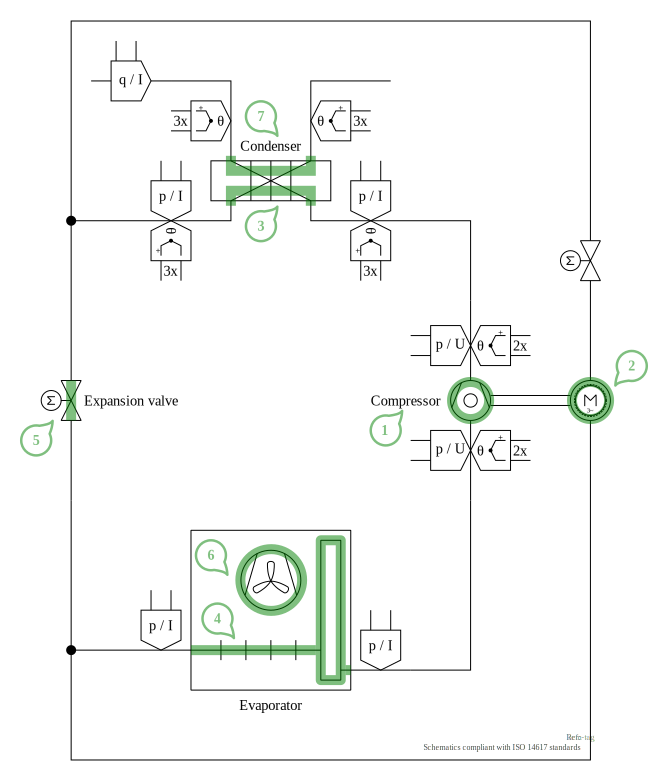
\includegraphics[width=0.9\textwidth]{simple-example-layout}
  \begin{tabular}[h]{cc}
    \includegraphics[width=0.45\textwidth]{simple-example-model} &
    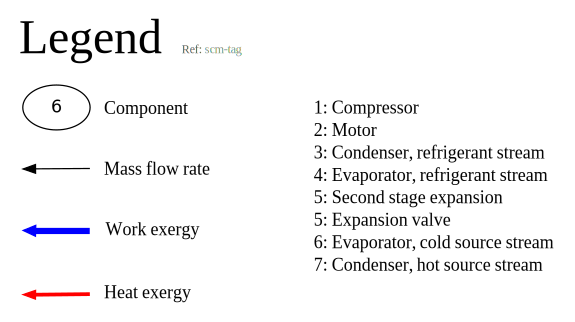
\includegraphics[width=0.45\textwidth]{simple-example-model-legend}\\
  \end{tabular}
  \caption[Example case -- Layout \& model]{Example case - Layout \&
    model of a single-stage heat pump. Symbols are compliant with the
    \cite{ISO14617}\,14617 standards.}
  \label{fig:simple-example-layout+model}
\end{figure}

The modeling methodology follows the steps detailed below:

\begin{description}
\item [Draw a layout of the installation and the frontier of the
  analysis]where appears \textbf{all} the flow rates and possible
  entities. Every flow rates need to be visible on the layout.
\item[Separate the layout in components.] A component is a network, as
  intended by \citet[p.\,24--25]{Borel-Favrat-2010a}, and corresponds
  to an element where flows enter and leave, partially (if there are
  accumulation) or totally, and that can exchange energy with normal
  components, or special components like the atmosphere or the
  environment of the device. The special components have no flow and
  are infinite reservoir at a given temperature. They can exchange
  energy with normal components or be the source or the receiver of
  flows. With this paradigm, a component does not necessarily
  correspond to a physical element or to a part of the system that can
  be isolated from the rest. For instance, a heat exchanger, in this
  paradigm, is made of two components which exchange heat energy. In
  the next chapters, the compression unit will be modeled as many
  components exchanging mass or energy (details about this modeling of
  the compression unit are given in \cref{chap:cp-intg}). This thesis
  work uses steady-state models. In steady state conditions, mass and
  energy balances are equal to zero for every components, as for the
  whole system delimited by a frontier. There is no mass change of the
  components. The components are assigned with a number. The modeling
  approach presented here could also be used to generate quasi-static
  models or dynamic models.
\item[Transform the layout view into the model view.] Each component
  exchanges energy or mass with other components. The representation
  of the model using the GraphViz modeling paradigm from
  \citet{Gansner-North-2000a}, typically dedicated to sofware
  engineering modeling, is unusual in the thermodynamic modeling field
  and is a representation analogy proposed by this thesis work. In the
  opposite, the modeling itself, using mass and energy balances is a
  common modeling approach in the thermodynamic field. Each type of
  energy is represented with a bold and colored arrow, and the mass
  flow rates are represented with thin black arrows. The convention is
  that positive energy or mass flow rates enter the
  components. Negative flows leave the components. This means that a
  negative value results in a flow moving against the arrow. The
  notation indicates the direction of the arrow with subscripts using
  the numbers or the components, separated by an arrow.
\item[Determine the equations.] Each components gives two equations: a
  mass flow rates balance equation, as detailled in
  \cref{eq:mass-balances-eq-general}, and an energy rates balance
  equation, as detailed in \cref{eq:energy-balances-eq-general}. By
  convention, each transformation energy rate\footnotep{See
    \cpref{sec:methodo-defs}, for a definition of the transformation
    energy rate.} is included in the equation using the outlet
  specific enthalpy\footnotep{See \cpref{sec:methodo-defs}, for a
    definition of the specific enthalpy.} of the component being the
  source of this flow rate. The whole device, at its frontier, also
  provides a mass flow rates balance equation and an energy rates
  balance equation. In the case of dynamic modeling, the mass and
  energy balance equations are not equal to zero. A steady-state
  approach has been favored in this thesis work because the data
  collected during the experiments were not sufficient to solve
  equations not equal to zero\footnotep{Fitting a dynamic model of the
    prototypes would have required to know the variation of mass of
    the components. Most of the components mass variation can be
    neglected, but the variation of mass of the condenser, the
    evaporator, and the economizer need to be measured (or,
    alternatively, the mass flow rates entering and leaving those
    components can be measured, but this is technically far more
    difficult and inconvenient). Those measurements were planned to be
    made in the BWP. Most of the experiments have been performed on
    the AWP. The BWP has only given a single OP and the load cells
    were not calibrated at the time, as this is a procedure which was
    planned for the next experiments. For more details, see
    \cpref{chap:awp}, and cpref{chap:bwp}.}.

\begin{equation}
  \label{eq:mass-balances-eq-general}
  \sum^n_{i=1} \dot{M}_{x_i \rightarrow y_i} = 0
  \tagaddtextone{$\left[\si{\watt}\right]$}
\end{equation}

\begin{equation}
  \label{eq:energy-balances-eq-general}
  \sum^m_{i=1} \dot{M}_{a_i \rightarrow b_i} \cdot h_{out\,a_i} +
  \sum^n_{j=1}\dot{Y}_{c_j \rightarrow d_j} +
  \sum^p_{k=1}\dot{E}_{e_k \rightarrow f_k} = 0
  \tagaddtextone{$\left[\si{\watt}\right]$}
\end{equation}

\item[Solve the system of equations.] Mass flow rate balance equation
  have the priority. They are solved first, if possible. When no more
  equations can be solved, a fitting parameter is added with the
  introduction of a new relation bounding 2 variables together. For
  instance, this can be introduced for a flow which is divided in
  two. The proportion of the entering flow leaving in one of the
  leaving flows is characterized here with a splitting parameter.

\item[Implement the model.] As soon as every variable can be
  expressed, the model is implemented in a modeling software (here,
  the MathWorks MATLAB) and the set of equation is solved with a
  solver. The solver tries to fit the parameter that were added to
  express every variable as an expression in order to get the lowest
  objective function value. If no fit parameter was added, the level
  of information of the system is sufficient and the set of equations
  should be closed, within the limits of the measurement uncertainty
  ranges. A set of equations is considered closed, in steady state
  conditions, if every energy and mass balance of every component and
  the balances at the frontier of the system are equal to zero. If fit
  parameters were added, the set of equations is now solvable but is
  not closed. Consequently, a fitting of those parameters is necessary
  to close the system. This step is performed using a minimization of
  an objective function under constraints, using a standard
  optimization algorithm. In this work, the MATLAB
  \textit{fmincon}\,\citep{fmincon2014a} function has been used with
  an interior point algorithm, which was the best suited to solve this
  problem \citep{fmincon2014a-interiorpoint} with this function. The
  variables of this algorithm are the fit parameters. The constraints
  on the variables are necessary to bound the fit parameters and to
  ensure that realistic conditions only are explored by the
  algorithm. For instance, if a flow is divided into three flows using
  two fit parameters, the sum of those two parameters can not be
  greater than one. The starting point of the minimization algorithm
  is determined randomly. The first valid starting point found
  randomly is selected as the optimization starting point. Indeed, the
  fluid properties at each location in the cycles are determined using
  the \REFPROP{} \citep{REFPROP90} but the latter can only compute
  properties within given inputs range. When the number of fit
  parameters starts to be quite high, as this is the case with the
  \AWP{} model, it is common that a randomly chosen starting point is
  not defined which implies that the minimization algorithm does not
  initialize. The objective function minimized by the optimizer is the
  sum of two aggregates of indicators. The first one has an order of
  magnitude above $\num{1e0}$ and is the sum of an array. This array
  contains statements penalizing unrealistic conditions in the system,
  such as an outlet stream enthalpy lower than its inlet stream
  enthalpy, in a compressor. If an unrealistic condition is observed,
  the objective function is penalized using the difference between the
  realistic condition that should be and its current unrealistic
  state. In other word, the more the condition is unrealistic the
  bigger is the penalization. This first term, as soon as the system
  is realistic, is equal to zero. If this term is not equal to zero,
  the solution found by the optimizer is not considered, an other
  starting point is chosen, and the optimizer is run again. The second
  term of the sum is of an order of magnitude below $\num{1e0}$ and
  corresponds to the sum of the energy balances on every component and
  on frontier of the system. It is equal to zero when all the balances
  are equal to zero. Typically, this term is never exactly equal to
  zero due to the fact that a model never fully represents the reality
  and due to uncertainties and measurement errors. The optimization
  problem has been run for every experimental points more that a
  hundred times in order to provide more confidence in the presented
  results. For the points presented in this work the sum of those
  balances is always below 100W.
\item[Analyze the results] As soon as the parameters of the system
  have been fitted, an analysis of the system can be performed.
\end{description}

In order to better understand this modeling approach, a simple example
dedicated to illustrate the methodology is offered here. The chosen
example is a single stage heat pump using part of the liquid
refrigerant leaving the condenser to cool down the motor of the
compressor. The partly evaporated flow is then collected at the
evaporator inlet. The layout of this heat pump is presented on
\cref{fig:simple-example-layout+model}. Using the modeling approach
proposed above, the example system is modeled using 7 components. This
model is described on \cref{fig:simple-example-layout+model}. The
components are represented on the layout with green markers and are
listed in the legend provided with the model.

Unfortunately, the designer of this example experimental setup, for
unknown reasons, could not instrument the heat pump with enough
sensors. Each component of the system can not be characterized and
only some physical values are available. The measurement points are
represented on the layout \cref{fig:simple-example-layout+model}. A
\gls{glos:bold} is a value physically measured in the experiment. An
\gls{glos:underline} is guessed directly by the optimizer, and a
\gls{glos:normal-font} is computed with the model\footnotep{See the
  glossary at the beginning of the thesis for details about the
  signification of those 3 types of values.}. The uncertainties are
being propagated through the model\footnotep{See \cpref{chap:uncert}
  for more details about uncertainties computation and
  propagation.}. For the example case, the values are presented in
\cref{tab:simple-example-PThs,tab:simple-example-dotEQ}.

\begin{table}[ht!]
  \footnotesize
  \begin{center}
    \begin{tabular}{cccccc}
\toprule
Component & Location & P / \si{\bar} & T / \si{\degreeCelsius} & h / \si{\kilo\joule\per\kilo\gram} & s / \si{\kilo\joule\per\kilo\gram\per\kelvin}\\
\midrule
\multirow{2}{*}{1} & inlet & \textbf{3.50 +/- 0.05} & \textbf{8.53 +/- 0.15} & 404.72 +/- 0.27 & 1.7359 +/- 0.0020\\
& outlet & \textbf{9.12 +/- 0.05} & \textbf{86.01 +/- 0.27} & 469.78 +/- 0.35 & 1.8689 +/- 0.0014\\
\midrule
\multirow{2}{*}{2} & inlet & \textbf{4.30 +/- 0.05} & 11.10 +/- 0.35 & 243.18 +/- 0.22 & 1.1526 +/- 0.0014\\
& outlet & \textbf{3.70 +/- 0.05} & 6.64 +/- 0.39 & 382.00 +/- 0.22 & 1.6507 +/- 0.0000\\
\midrule
\multirow{2}{*}{3} & inlet & \textbf{9.12 +/- 0.05} & \textbf{86.01 +/- 0.15} & 469.78 +/- 0.22 & 1.8689 +/- 0.0010\\
& outlet & \textbf{8.52 +/- 0.05} & \textbf{31.01 +/- 0.15} & 243.18 +/- 0.22 & 1.1481 +/- 0.0007\\
\midrule
\multirow{2}{*}{4} & inlet & \textbf{3.70 +/- 0.05} & 6.64 +/- 0.39 & 245.81 +/- 17.47 & 1.1639 +/- 0.0015\\
& outlet & \textbf{3.50 +/- 0.05} & 8.53 +/- 0.44 & 404.72 +/- 0.27 & 1.7359 +/- 0.0020\\
\midrule
\multirow{2}{*}{5} & inlet & 8.52 +/- 0.05 & 31.01 +/- 0.15 & 243.18 +/- 0.22 & 1.1481 +/- 0.0007\\
& outlet & 3.70 +/- 0.05 & 6.64 +/- 0.39 & 243.18 +/- 0.22 & 1.1545 +/- 0.0015\\
\midrule
\multirow{2}{*}{6} & inlet & \textbf{1.00 +/- 0.05} & \textbf{10.00 +/- 0.15} & 407.21 +/- 0.16 & 3.8055 +/- 0.0149\\
& outlet & \textbf{1.00 +/- 0.05} & \textbf{7.00 +/- 0.15} & 404.20 +/- 0.16 & 3.7948 +/- 0.0149\\
\midrule
\multirow{2}{*}{7} & inlet & \textbf{2.00 +/- 0.05} & \textbf{30.00 +/- 0.15} & 125.91 +/- 0.63 & 0.4367 +/- 0.0021\\
& outlet & \textbf{1.70 +/- 0.05} & \textbf{35.00 +/- 0.15} & 146.78 +/- 0.63 & 0.5051 +/- 0.0020\\
\bottomrule
\end{tabular}

  \end{center}
  \caption{Example case -- Thermodynamic points of the heat pump cycle}
  \label{tab:simple-example-PThs}
\end{table}

In order to compensate for the missing measurements, the heat pump
system is modeled with the proposed approach. The known mass flows and
energy fluxes are identified and used to write the set of equations in
a solvable order. The set of equations is detailed for this example
case in \cpref{chap:simple-model-equations-set}. The set of equations
is solved, starting with mass flow rates balance equations. When the
resolution is stopped by uncharacterized flows, a fit parameter is
added. For instance, in the example case, the refrigerant flow coming
from the compressor (component \#1) is divided after the condenser
circuit (component \#3) into two streams. The splitting of this flow
between those two streams is unknown. Consequently, a split factor is
added and will later be fitted in order to close the set of equations
(in the example case, the fit parameter $f_{01}$ is introduced
with \cref{eq:simple-model-equations-set-factor01}). As soon as every
mass flow is characterized, eventually using fit parameters, the same
procedure is applied to energy fluxes, starting with known fluxes, and
using equations similar to \cref{eq:energy-balances-eq-general}. When
the resolution is stopped by uncharacterized fluxes, a fit parameter
is also added. At the end of this process, the whole system is
characterized using the thermodynamic conditions at the measurement
points and the measured flows and fluxes. In the example case
considered in this chapter, this model allows to determine the values
presented in
\crefrange{tab:simple-example-PThs}{tab:simple-example-dotEQ}, to draw
diagrams such as the ones presented
\cref{fig:simple-example-diagrams}, and to determine performance
indicators, such as the \COP{}, which is here of 3.35, or such as the
motor efficiency, which is here of~\SI{96.11}{\%}\footnotep{Those
  performance indicators are defined in section
  \cref{sec:methodo-analysis}.}.

\begin{table}[htb]
    \footnotesize
    \begin{center}
    \begin{tabular}{llllll}
\toprule
Name & Value / \si{\gram\per\second} & Name & Value / \si{\gram\per\second} & Name & Value / \si{\gram\per\second} \\
\midrule
$\dot{M}_{1 \rightarrow 3}$ & 32.2336 +/- 1.65904 & $\dot{M}_{2 \rightarrow 4}$ & 0.611456 +/- 0.0314711 & $\dot{M}_{3 \rightarrow 2}$ & 0.611456 +/- 0.0314711 \\
$\dot{M}_{3 \rightarrow 5}$ & 31.6221 +/- 1.62757 & $\dot{M}_{4 \rightarrow 1}$ & 32.2336 +/- 1.62787 & $\dot{M}_{5 \rightarrow 4}$ & 31.6221 +/- 1.62757 \\
$\dot{M}_{6 \rightarrow en}$ & 1697.52 +/- 180.24 & $\dot{M}_{7 \rightarrow ho}$ & \textbf{350 +/- 10} & $\dot{M}_{en \rightarrow 6}$ & 1697.52 +/- 180.24 \\
$\dot{M}_{ho \rightarrow 7}$ & 350 +/- 10 \\
\bottomrule
\end{tabular}

  \end{center}
  \caption{Example case -- Mass flow rates between the components}
  \label{tab:simple-example-dotM}
\end{table}

\begin{table}[htb]
    \footnotesize
    \begin{center}
    \begin{tabular}{llll}
\toprule
Name & Value / $W$ & Name & Value / $W$ \\
\midrule
$\dot{E}_{2 \rightarrow 1}$ & 2097.11 +/- 108.52 & $\dot{E}_{el \rightarrow 2}$ & \textbf{2182.00 +/- 1.00} \\
$\dot{Y}_{3 \rightarrow 7}$ & 7304.18 +/- 375.81 & $\dot{Y}_{6 \rightarrow 4}$ & 5122.18 +/- 375.81 \\
\bottomrule
\end{tabular}

  \end{center}
  \caption{Example case -- Energy flows between the components}
  \label{tab:simple-example-dotEQ}
\end{table}

\begin{figure}[htb]
  \centering
  \subfloat[Refrigeration diagram]
  {\label{fig:simple-example-Ph}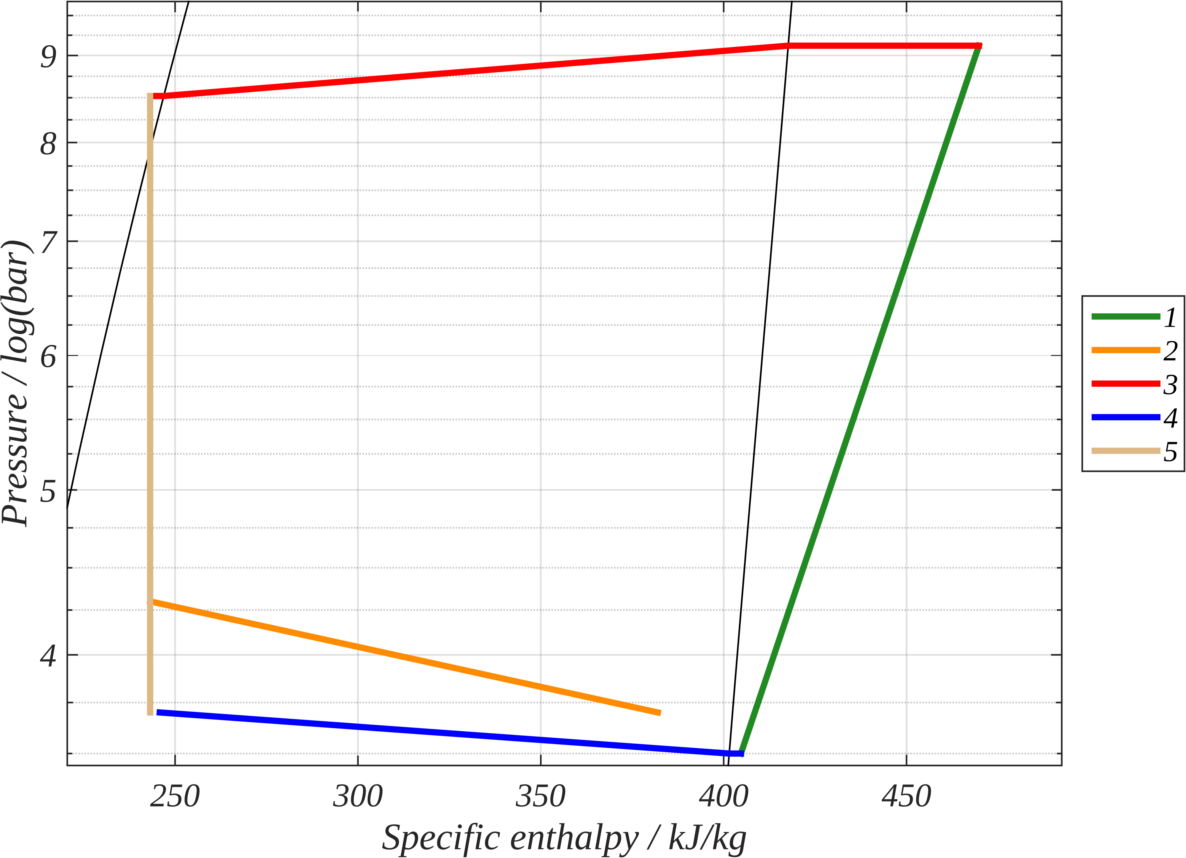
\includegraphics[width=0.45\textwidth]{simple-example-Ph}}
  \hspace{1em}
  \subfloat[Entropic diagram]
  {\label{fig:simple-example-Ts}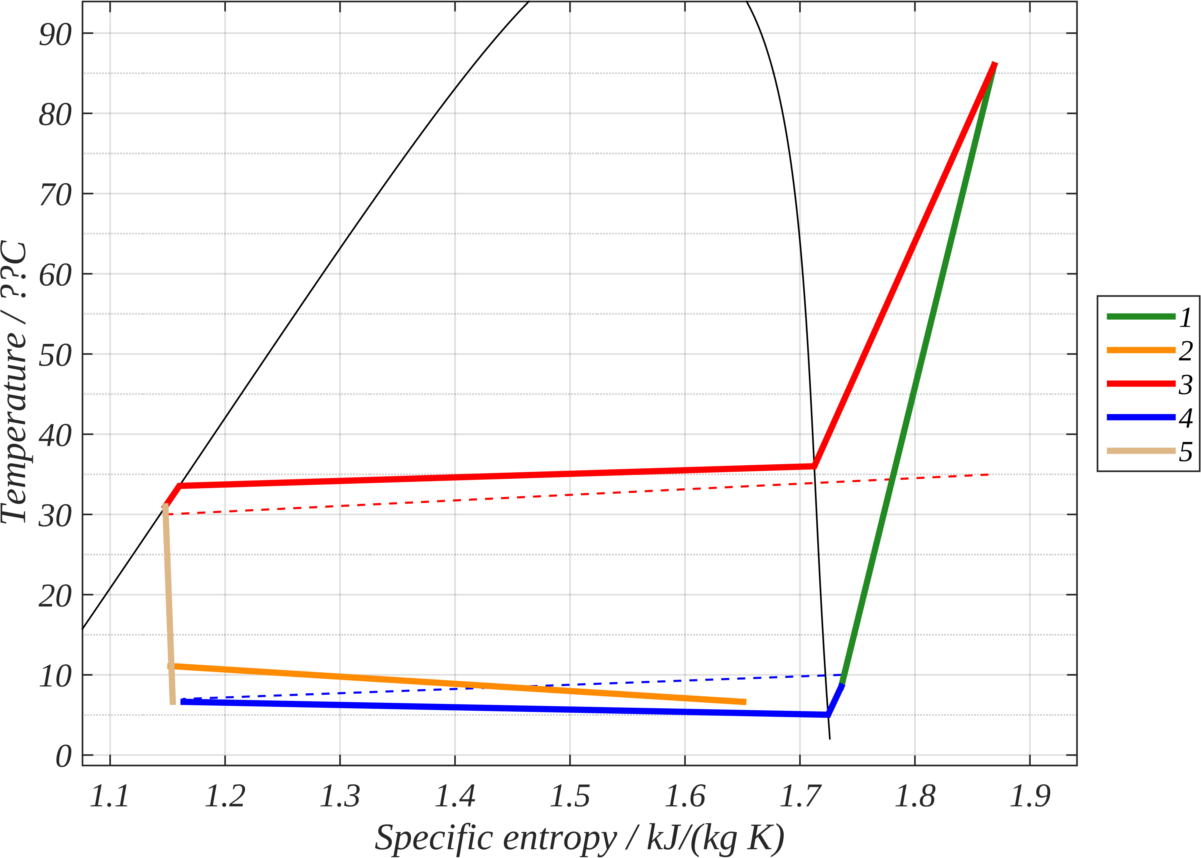
\includegraphics[width=0.45\textwidth]{simple-example-Ts}}
  \caption[Example case -- Thermodynamic diagrams]{Example case --
    Thermodynamic diagrams. The legend of the numbered lines is
    available on \cref{fig:simple-example-layout+model}. Dashed lines
    represent the sources.}
  \label{fig:simple-example-diagrams}
\end{figure}

\subsection{Analysis of the experimental results}
\label{sec:methodo-analysis}

The experimental results are analyzed using diagrams, and performance
indicators, which are defined below.

\subsubsection{Definitions}
\label{sec:methodo-defs}

\paragraph{Pressure ratio ($\Pi$)}

The pressure ratio is the ratio of the absolute pressure at the
compressor outlet to the absolute pressure at the compressor
inlet. Consequently first stage pressure ratio is the ratio of the
absolute pressure at the first stage compressor outlet $P_{1,\,out}$
to the absolute pressure at the first-stage compressor inlet
$P_{1,\,in}$. The second stage pressure ratio is the ratio of the
absolute pressure at the second stage compressor outlet $P_{2,\,out}$
to the absolute pressure at the second stage compressor inlet
$P_{2,\,in}$. Those two ratios are defined in \cref{eq:PR}.

\begin{subequations}
  \label{eq:PR}
  \begin{align}
  \Pi_1 = \dfrac{P_{1,\,out}}{P_{1,\,in}}
  \tagaddtexttwo{$\left[-\right]$} \\
  \Pi_2 = \dfrac{P_{2,\,out}}{P_{2,\,in}}
  \tagaddtexttwo{$\left[-\right]$}
  \end{align}
\end{subequations}

% \paragraph{Mass flow rate ($\dot{M}$)}


\paragraph{Specific enthalpy ($h$)}

The specific enthalpy is a state function resulting of the combination
of the specific internal energy $u$, the specific volume $v$, and the
pressure $P$ state functions \citep[p.\,19]{Borel-Favrat-2010a}. It is
computed as described in \cref{eq:h}. The specific enthalpy is used in
the energy rate calculations.

\begin{equation}
  \label{eq:h}
  h = u + vP
  \tagaddtextone{$\left[\si{\joule\per\kilo\gram}\right]$}
\end{equation}

\paragraph{Specific entropy ($s$)}
The specific entropy is a state function which may vary as a result of
transfers across the system boundary or because of internal processes
of the system which result in entropy creation
\citep[p.\,37]{Borel-Favrat-2010a}. The specific entropy unit is
\si{\joule\per\kilo\gram\per\kelvin}. It is used in various
thermodynamic calculations, and especially in exergy calculation, via
the coenthalpy.


\paragraph{Specific coenthalpy ($k$)}
The specific coenthalpy is a state function defined from the specific
enthalpy $h$, the environment temperature $T_a$ and the specific
entropy $s$, as described in \cref{eq:k}
\citep[p.\,410]{Borel-Favrat-2010a}. The specific coenthalpy is used in
the exergy rate calculations.

\begin{equation}
  \label{eq:k}
  k = h + T_as
  \tagaddtextone{$\left[\si{\joule\per\kilo\gram}\right]$}
\end{equation}

\paragraph{Transformation energy rate ($\dot{Y}$)}

\citet[p.\,24]{Borel-Favrat-2010a} define the transformation energy
rate as defined in \cref{eq:dotY}. Normally, the transformation energy
rate is decreased by the derivative of the quantity $U + P_aV$,
relative to time, $U$ being the internal energy, $P_a$ being the
pressure of the environment, and $V$ being the volume. The derivative
of this quantity being equal to zero or being negligible for the
system studied here, it is not mentioned in \cref{eq:dotY}.

\begin{equation}
  \label{eq:dotY}
  \dot{Y}^{+} = \sum_{j} h_j \, \dot{M}_j^{+}
  \tagaddtextone{$\left[\si{\watt}\right]$}
\end{equation}

\paragraph{Transformation exergy rate ($\dot{E}_{y}$)}

Based on the transformation energy rate, the transformation exergy
rate is defined as described in \cref{eq:dotEy}
\citep[p.\,410]{Borel-Favrat-2010a}. Normally, the transformation
exergy rate is decreased by the derivative of coenergy $J$ relative to
time. The coenergy is defined as $J = U + P_aV-T_aS$ with $U$, the
internal energy, $P_a$ the environment pressure, $T_a$, the
environment temperature, $V$, the volume, and $S$, the entropy. The
derivative of this quantity being here equal to zero or being
negligible for the system being studied here, it is not mentioned in
\cref{eq:dotEy}.

\begin{equation}
  \label{eq:dotEy}
  \dot{E}_{y}^{+} = \sum_{j} k_j \, \dot{M}_j^{+}
  \tagaddtextone{$\left[\si{\watt}\right]$}
\end{equation}

\subsubsection{Performance indicators}
\label{sec:methodo-indicators}

\paragraph{Heating effectiveness ($COP_h$)}

The heating effectiveness $\epsilon_h$, also called heating
Coefficient Of Performance ($COP_h$), is the ratio between heat power
$\dot{Q}^{-}_h$ supplied to the hot source and the consumed work power
$\dot{E}^{+}$. This definition can also be given in energy instead of
power, as defined by \citet[p.\,641]{Borel-Favrat-2010a}. It is
defined in \cref{eq:COPh}.

\begin{equation}
  \label{eq:COPh}
  \epsilon_h = COP_h = \dfrac{\dot{Y}^{-}_h}{\dot{E}^{+}} = \dfrac{\dot{Y}^{-}_{3 \rightarrow 15}}{\dot{E}^{+}_{el \rightarrow 14}}
  \tagaddtextone{$\left[-\right]$}
\end{equation}

\paragraph{Motor efficiency ($\eta_{mot}$)}

The motor efficiency is defined as the ratio between the work
transmitted to the shaft $\dot{E}^-_{\text{shaft}}$ and the electric
power consumed by the motor $\dot{E}^+_{\text{mot}}$. It is defined in
\cref{eq:eta_mot}.

\begin{equation}
  \label{eq:eta_mot}
  \eta_{mot} = \dfrac{\dot{E}^-_{\text{shaft}}}{\dot{E}^+_{\text{mot}}}
  \tagaddtextone{$\left[-\right]$}
\end{equation}

% \paragraph{Gas bearings effectiveness}

\paragraph{Isentropic efficiency ($\eta_s$)}

The isentropic efficiency of a compressor is defined as the ratio
between the isentropic work power of the compressor $\dot{E}_{cp,s}$,
which is the work power required by a compressor adiabatic and without
dissipation performing an isentropic compression, and the actual work
$\dot{E}_{cp}$ required by the compressor. It is defined by
\cref{eq:eta_s_cp}.

\begin{equation}
  \label{eq:eta_s_cp}
  \eta_s = \dfrac{\dot{E}_{cp,s}}{\dot{E}_{cp}} = \dfrac{h_{out,s} - h_{in}}
  {h_{out} - h_{in}}
  \tagaddtextone{$\left[ - \right]$}
\end{equation}

The compressor inlet specific enthalpy $h_{in}$ is computed using the
inlet absolute pressure $P_{in}$ and temperature $T_{in}$. The
compressor isentropic outlet specific enthalpy $h_{out,s}$ is computed
using the outlet absolute pressure $P_{out}$ and the inlet specific
entropy $s_{in}$. The compressor outlet specific enthalpy $h_{out}$ is
computed using the inlet absolute pressure $P_{out}$ and temperature
$T_{out} > T_{out,s}$. The isentropic efficiency ranges between 0 and
1 (1 is the ideal unreachable case) and typical values range between
0.7 and 0.8 for nowadays compressors.

In the specific case of the non-adiabatic compression unit tested, we
can differentiate the external isentropic efficiency, and the
isentropic efficiency of the impeller only. The isentropic efficiency
of the impeller only is not accurately known, as the inlets and
outlets temperatures and pressure levels are deduced from the models
presented \cref{sec:awp-model,sec:bwp-model} and not measured
directly. They are defined with \cref{eq:eps_cp1_s,eq:eps_cp2_s}. The
external isentropic efficiencies include the leakage through the
labyrinth seal and the gas flux from the axial bearing to the inlet of
the first impeller. They are the isentropic efficiencies as measurable
from the outside of the unit, at its physical inlets/outlets. Those
isentropic efficiencies are defined in
\cref{eq:eps_cp1_s_ext,eq:eps_cp2_s_ext} and are based on the
definition offered by \citet[p.\,201]{Borel-Favrat-2010a}.

\begin{equation}
  \label{eq:eps_cp1_s}
  \eta_{s,\,cp1} = \dfrac{\dotM{29}{1} \, h_{1,\,out,\,s} -
    \dotM{29}{1} \, h_{1,\,in} + \dot{Q}_{11 \rightarrow 1} -
    \dot{Q}_{1 \rightarrow 2}}{\dotM{29}{1} \, h_{1,\,out} - \dotM{29}{1} \,
    h_{1,\,in} + \dot{Q}_{11 \rightarrow 1} - \dot{Q}_{1 \rightarrow 2}}
  \tagaddtextone{$\left[-\right]$}
\end{equation}

\begin{equation}
  \label{eq:eps_cp1_s_ext}
  \eta_{s,\,cp1,\,ext} = \dfrac{\left( \dotM{10}{25} + \dotM{25}{27} +
      \dotM{25}{8} \right) \, h_{1,\,out,\,s} - \dotM{22}{29} \,
    h_{22,\,out} + \dot{Q}_{11 \rightarrow 1} - \dot{Q}_{1
      \rightarrow 2}}{\left( \dotM{10}{25} + \dotM{25}{27} +
      \dotM{25}{8} \right) \, h_{1,\,out} - \dotM{22}{29} \,
    h_{22,\,out} + \dot{Q}_{11 \rightarrow 1} - \dot{Q}_{1
      \rightarrow 2}}
  \tagaddtextone{$\left[-\right]$}
\end{equation}

\begin{equation}
  \label{eq:eps_cp2_s}
  \eta_{s,\,cp2} = \dfrac{\dotM{28}{2} \, h_{2,\,out,\,s} - \dotM{28}{2}
    h_{2,\,in} + \dot{Q}_{1 \rightarrow 2} - \dot{Q}_{2 \rightarrow
      10}}{\dotM{28}{2} \, h_{2,\,out} - \dotM{28}{2} h_{2,\,in} +
    \dot{Q}_{1 \rightarrow 2} - \dot{Q}_{2 \rightarrow 10}}
  \tagaddtextone{$\left[-\right]$}
\end{equation}

\begin{equation}
  \label{eq:eps_cp2_s_ext}
  \eta_{s,\,cp2,\,ext} = \dfrac{\left( \dotM{2}{10} + \dotM{2}{20}
    \right) \, h_{2,\,out,\,s} - \dotM{28}{2} \, h_{2,\,in} +
    \dot{Q}_{1 \rightarrow 2} - \dot{Q}_{2 \rightarrow 10}}{\left(
      \dotM{2}{10} + \dotM{2}{20} \right) \, h_{2,\,out} -
    \dotM{28}{2} \, h_{2,\,in} + \dot{Q}_{1 \rightarrow 2} -
    \dot{Q}_{2 \rightarrow 10}}
  \tagaddtexttwo{$\left[-\right]$}
\end{equation}

\paragraph{Exergy efficiencies ($\eta$)}

\citet[based on def.~p.\,2]{Favrat-Epelly-2008a} give a general
definition of the exergy linked to a transfer or a storage of energy
and defined it as the potential of maximum work which could ideally be
obtained from each energy unit being transferred or stored (using
reversible processes exchanging heat only with the
atmosphere). \citet[p.\,406--448]{Borel-Favrat-2010a} give a detailed
explanation of the exergy approach applied to system analysis. They
develop the concept of exergy efficiency in general
\citep[p.\,447--448]{Borel-Favrat-2010a}, and apply it to the specific
case of a heat pump \citep[p.\,642]{Borel-Favrat-2010a}. Written using
exergy rates instead exergy, the exergy efficiency of a heat pump is
defined as the ratio between the supplied transformation exergy power
$\dot{E}^-_{yh}$ and the consumed electrical power
$\dot{E}^+_{el}$. This ratio is expressed mathematically in
\cref{eq:eta_heatpump}.

\begin{equation}
  \label{eq:eta_heatpump}
  \eta_{heatpump} = \dfrac{\dot{E}^-_{yh}}{\dot{E}^+_{el}} =
  \dfrac{\dotM{17}{15} \, \left( k_{15,\,out} - k_{15,\,in} \right)}
  {\dotE{el}{14}}
  \tagaddtexttwo{$\left[-\right]$}
\end{equation}


The exergy efficiency of the first compression stage is defined in \cref{eq:eta_cp1_awp} for the \AWP{}, and in \cref{eq:eta_cp1_bwp} for the \BWP{}.

\begin{subequations}
  \begin{align}
  \eta_{cp1} = \dfrac{\dotM{22}{29} \, \left( k_{25,\,out} - k_{29,\,in} \right)}{\dotE{11}{1} - \dotE{1}{2}}
  \tagaddtextthree{$\left[-\right]$} \label{eq:eta_cp1_awp} \\
  \eta_{cp1} = \dfrac{\dotM{19}{1} \, \left( k_{25,\,out} - k_{19,\,out} \right)}{\dotE{11}{1} - \dotE{1}{2}}
  \tagaddtextthree{$\left[-\right]$} \label{eq:eta_cp1_bwp}
  \end{align}
\end{subequations}

The exergy efficiency of the first stage impeller is defined in
\cref{eq:eta_cp1_imp}.

\begin{equation}
  \label{eq:eta_cp1_imp}
  \eta_{cp1,\,imp} = \dfrac{\dotM{1}{25} \, \left( k_{1,\,out} - k_{1,\,in} \right)}{\dotE{11}{1} - \dotE{1}{2}}
  \tagaddtexttwo{$\left[-\right]$}
\end{equation}

The exergy efficiency of the second compression stage is defined in
\cref{eq:eta_cp2}.

\begin{equation}
  \label{eq:eta_cp2}
  \eta_{cp2} = \dfrac{\dotM{2}{20} \, \left( k_{2,\,out} - k_{2,\,in} \right)}{\dotE{1}{2}}
  \tagaddtexttwo{$\left[-\right]$}
\end{equation}

The exergy efficiency of the second stage impeller is defined in
\cref{eq:eta_cp2_imp_awp} for the \AWP{}, and in
\cref{eq:eta_cp2_imp_awp} for the \BWP{}.

\begin{subequations}
  \begin{align}
    \eta_{cp2,\,imp} = \dfrac{\dotM{28}{2} \, \left( k_{2,\,out} - k_{2,\,in} \right)}{\dotE{1}{2}}
    \tagaddtextthree{$\left[-\right]$} \label{eq:eta_cp2_imp_awp} \\
    \eta_{cp2,\,imp} = \dfrac{\dotM{27}{2} \, \left( k_{2,\,out} - k_{2,\,in} \right)}{\dotE{1}{2}}
    \tagaddtextthree{$\left[-\right]$} \label{eq:eta_cp2_imp_bwp}
  \end{align}
\end{subequations}

Component \#15 specific coenthalpies are determined using CoolProp
5.0.8 \citep{coolprop} Ethylen Glycol / Water mixture fluid
properties. Other fluid properties are computed using \REFPROP{}
\citep{REFPROP90}. The exergy efficiency of condenser is defined in \cref{eq:eta_cd}.

\begin{equation}
  \label{eq:eta_cd}
  \eta_{cd} = \dfrac{\dotM{20}{3} \, \left( k_{3,\,in} - k_{3,\,out} \right)}{\dotM{17}{15} \, \left( k_{15,\,out} - k_{15,\,in} \right)}
  \tagaddtexttwo{$\left[-\right]$}
\end{equation}

The exergy efficiency of evaporator is defined in \cref{eq:eta_ev_awp}
for the \AWP{}, and in \cref{eq:eta_ev_bwp} for the \BWP{}.

\begin{subequations}
  \begin{align}
    \eta_{ev} = \dfrac{\dotM{env}{16} \, \left( k_{16,\,in} - k_{16,\,out} \right)}{\dotM{9}{4} \, \left( k_{4,\,out} - k_{4,\,in} \right)}
    \tagaddtextthree{$\left[-\right]$} \label{eq:eta_ev_awp} \\
    \eta_{ev} = \dfrac{\dotM{18}{16} \, \left( k_{16,\,in} - k_{16,\,out} \right)}{\dotM{4}{19} \, \left( k_{4,\,out} - k_{4,\,in} \right)}
    \tagaddtextthree{$\left[-\right]$} \label{eq:eta_ev_bwp}
  \end{align}
\end{subequations}

The exergy efficiency of subcooler is defined in \cref{eq:eta_sc}.

\begin{equation}
  \label{eq:eta_sc}
  \eta_{sc} = \dfrac{\dotM{19}{6} \, \left( k_{19,\,in} - k_{19,\,out} \right)}{\dotM{18}{22} \, \left( k_{18,\,in} - k_{18,\,out} \right)}
  \tagaddtexttwo{$\left[-\right]$}
\end{equation}

The exergy efficiency of the mechanical transmission in the
compression unit is defined in \cref{eq:eta_trans}.

\begin{equation}
  \label{eq:eta_trans}
  \eta_{trans} = \dfrac{\dotE{11}{1}}{\dotE{13}{12}}
  \tagaddtexttwo{$\left[-\right]$}
\end{equation}

The exergy efficiency of the motor in the compression unit is defined
in \cref{eq:eta_mot}.

\begin{equation}
  \label{eq:eta_mot}
  \eta_{mot} = \dfrac{\dotE{13}{12} + \dotM{3}{7} \, \left( k_{7,\,out} - k_{7,\,in} \right)}{\dotE{14}{13}}
  \tagaddtexttwo{$\left[-\right]$}
\end{equation}

\subsubsection{Diagrams}
\label{sec:methodo-diagrams}

\paragraph{Refrigeration diagram}

A refrigeration diagram is a diagram that represents a thermodynamic
cycle and the state of the refrigerant on a two-dimension space. The
abscissa is specific enthalpy, and the ordinate is the logarithm of
the absolute pressure
\citep[p.\,370--373]{Borel-Favrat-2010a}. \Cref{fig:simple-example-Ph}
shows an example of refrigeration diagram.

\paragraph{Entropic diagram}

An entropic diagram is a diagram that represents a thermodynamic cycle
and the state of the refrigerant on a two-dimension space. The
abscissa is specific entropy, and the ordinate temperature
\citep[p.\,355--361]{Borel-Favrat-2010a}. \Cref{fig:simple-example-Ts}
shows an example of entropic diagram.

\paragraph{Sankey energy diagram}

A Sankey diagram is a flow diagram in which the width of the arrows is
shown proportionally to the flow quantity. Sankey diagrams are
typically used to visualize energy, material, or cost transfers
between processes. \cpref{fig:awp-A-7.0/W35.6-sankey-energy}, shows an
example of Sankey energy diagram.

\FloatBarrier
\bibliographystyle{plainnat}
\bibliography{main}
\label{sec:methodo-refs}


%% Air-Water twin-stage oil-free domestic heat pump
%% Description, modeling, and results
\chapter{Air-Water heat pump Prototype (AWP)}
\label{chap:awp}
\resetallacronyms

\begin{shaded}
  This chapter presents the \AWP{} designed to demonstrate the
  statement detailed in \cref{chap:methodo}. It presents the prototype
  specifications and design, its results, and the encountered issues.
\end{shaded}

\section{Design of the AWP}
\label{sec:awp-design}

\subsection{Specifications}
\label{sec:awp-specs}

The prototype specifications were:
\begin{description}
\item[Efficiency] The prototype had to demonstrate the potential of an
  oil-free radial variable-speed multi-stage compressor unit for
  domestic heat pumps applications.
\item[Compactness] The prototype had to fit into the housing of the
  existing Air-Water heat pump, pictured in \cref{fig:awp-housing},
  chosen and provided by the industrial partner.
\item[Low cost] The prototype was intended to demonstrate the
  simplicity of the heat pump layout selected, which would have had
  positive effects on the costs of the industrial
  product\footnotep{The choice of the two-stage heat pump layout is
    discussed in \cpref{sec:sota-multistage}.}. The selected layout is among the simplest
  possible layouts.
\end{description}

Those 3 guidelines led to the following design choices:
\begin{description}
\item[Basic measurements capability] The prototype was intended to be
  equipped only with pressure and temperature sensors in order to get
  close to the compactness of an industrial product and to limit the
  costs of the prototype itself. Originally, none of the prototype
  internal refrigerant flow rates were measured. The only flow rate
  being measured was the water flow rate at the condenser. With the
  issues encountered during the tests\footnotep{The issues encountered
    during the tests are detailed in \cpref{sec:awp-perfs}, and
    \cpref{sec:awp-control-issues}.}, Coriolis mass flow meters were
  added on the motor cooling refrigerant flow and on the gas bearings
  aeration refrigerant flow. The flow rates in the main circuits were
  not measured and were deduced from the condenser energy
  balance\footnotep{See \crefrange{eq:cd-eb-01}{eq:cd-eb-03}
    page~\pageref{eq:cd-eb-01} for details about the AWP condenser
    energy balance.} and from the global energy balance\footnotep{See
    \cref{eq:ev-eb-01,eq:ev-eb-02}, page~\pageref{eq:ev-eb-01}
    for details about the AWP global energy balance.}, in steady state
  conditions.
\item[Components merged together] The
  \gls{glos:economizer}\index{economizer} has been merged with the
  volute of the compression unit in order to obtain one element
  only. Details about this component merging are given in
  \cref{sec:awp-eco}.
\item[Compact cycle inversion circuit] The circuit for the cycle
  inversion, in this twin-stage heat pump, meant for defrosting the
  evaporator or for cooling applications, is made with a set of 4
  check valves\footnotep{The 4 check valves are easily seen on
    \cref{fig:awp_assembly_3} page~\pageref{fig:awp_assembly_3}.} and a
  4-way valve\footnotep{The 4-way valve can be seen on
    \cref{fig:awp_assembly_2} page~\pageref{fig:awp_assembly_2}.},
  which makes it very compact. This circuit and cycle inversion
  solution can be observed on \cref{fig:awp-layout-model-numbers}.
\end{description}

\subsection{Description}
\label{sec:awp-description}

The \AWP{} is the second prototype to be built\footnotep{See
  \cpref{sec:potential-demo} for details about the timeline of the
  experimental setups in the project.} and has been designed to be
integrated into one of the industrial partner's single-stage Air/Water
heat pump housing. The industrial partner's Air-Water heat pumps are
designed for cold climates. Consequently, their heat pump circuits and
components are located below the air ducting, which is made of the
ducting itself, the fan, and the evaporator, as illustrated in
\cref{fig:awp-housing}. This design allows to keep the air ducting
above snow level. As a consequence of this design choice, the heat
pump layout topology for the \AWP{} had to fit into the space
available below the air ducting, as illustrated in
\cref{fig:awp-housing,fig:awp-3d-layout}. The topology of the \AWP{},
designed to fit into the volume available under the air ducting can be
seen in \cref{fig:awp-3d-layout}.

\begin{figure}[htbp]
  \centering \subfloat[Heat pump air ducting and housing]{\label{fig:awp-housing}
    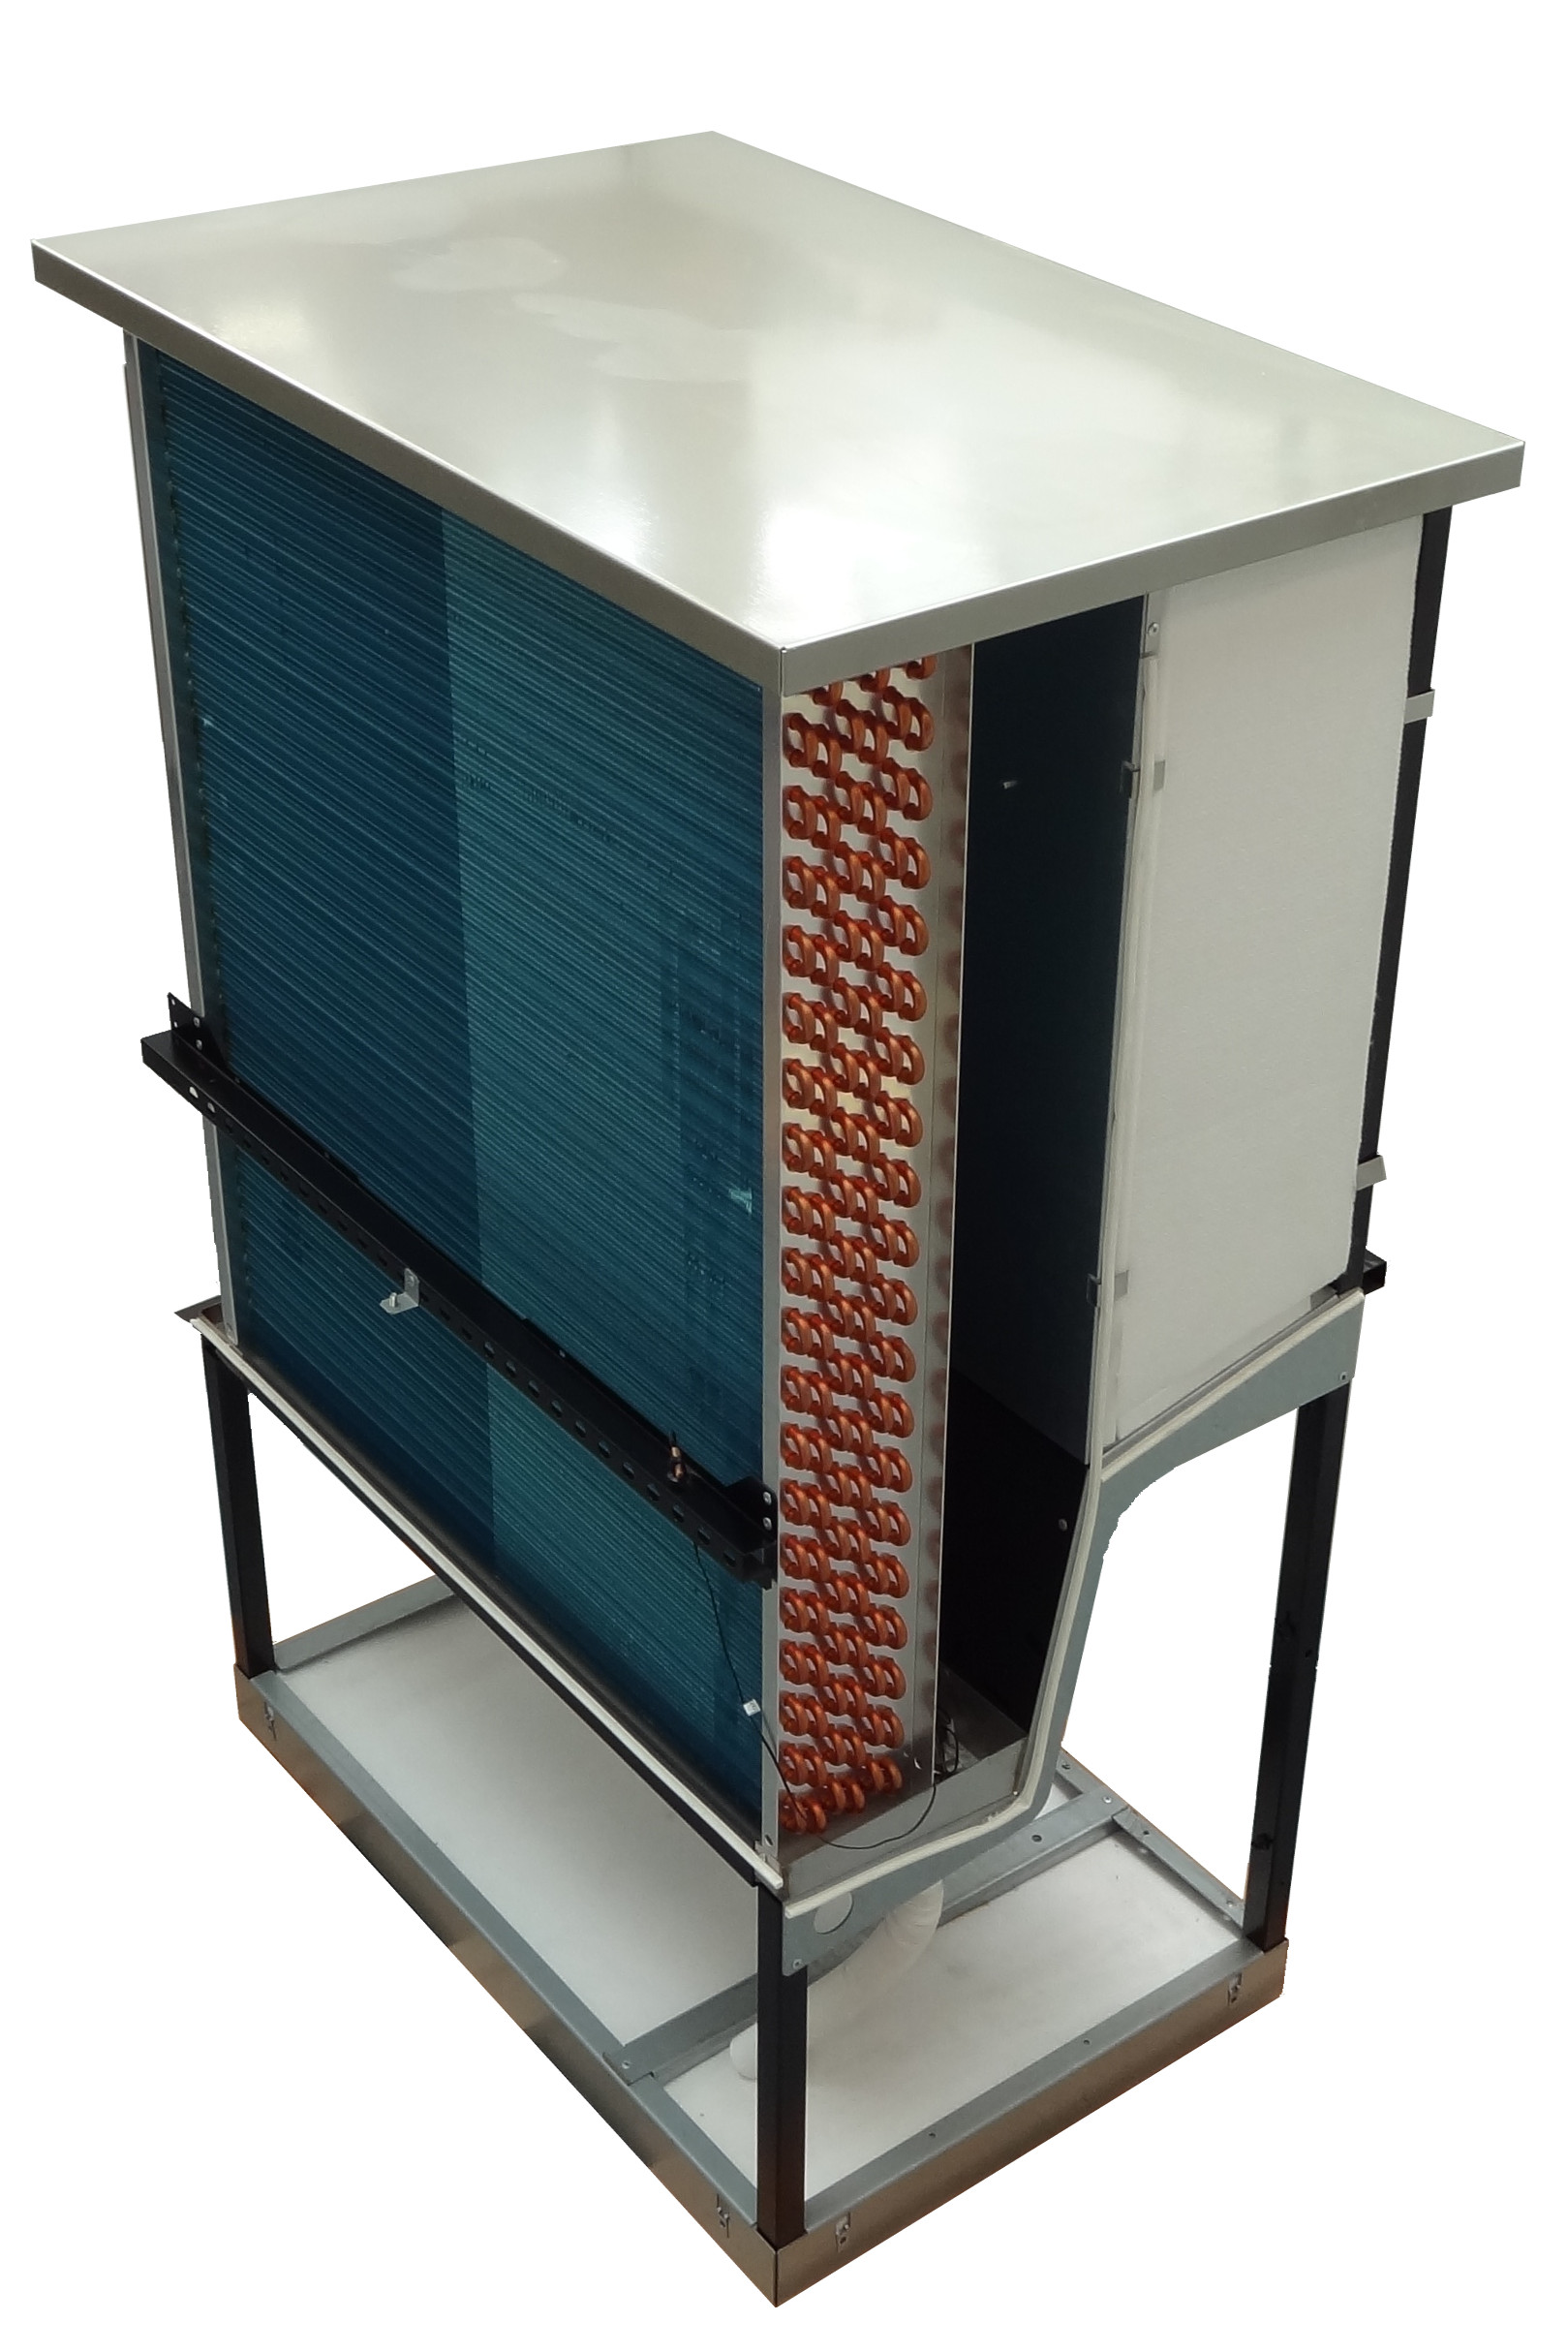
\includegraphics[height=8cm]{awp-chassis}}
  \subfloat[AWP 3D layout (bottom part)]{
    \label{fig:awp-3d-layout}
    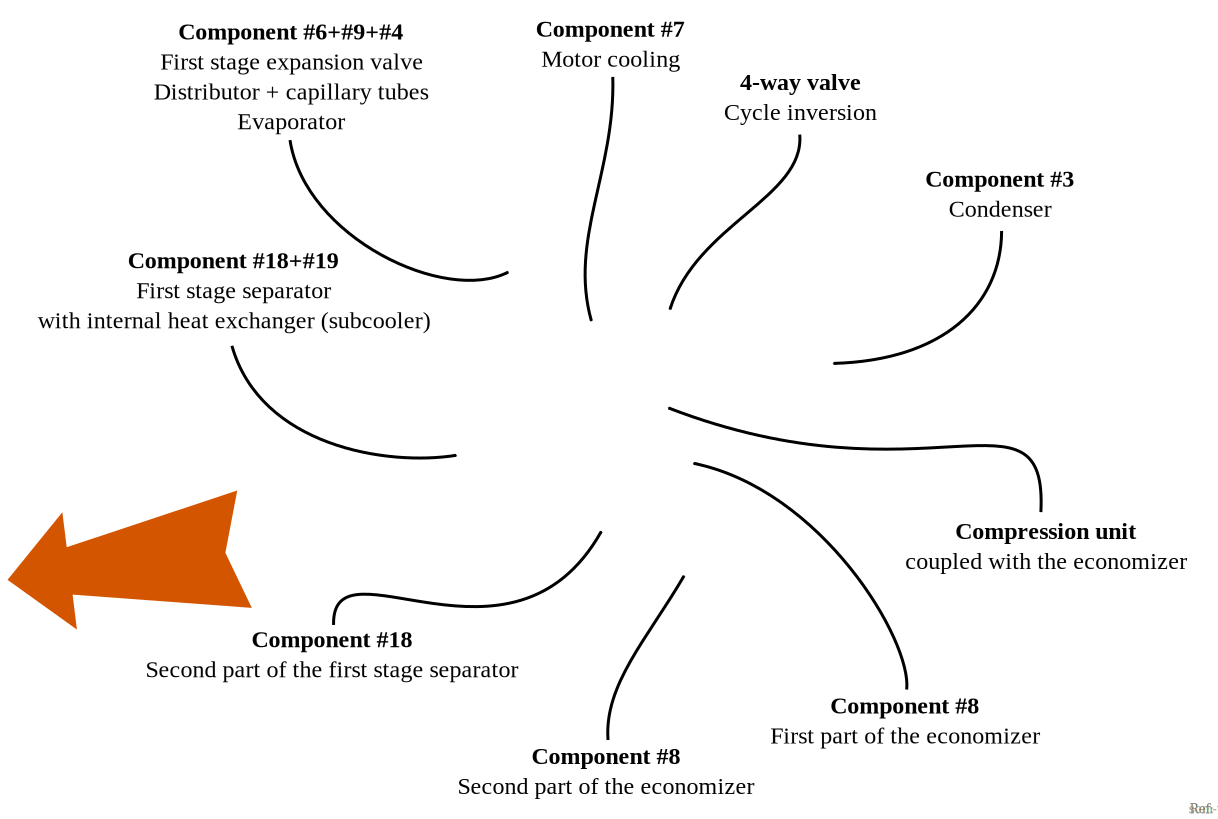
\includegraphics[height=7cm]{awp-3d-layout-commented}}
  \caption[Housing and 3D layout of the AWP circuits]{Housing and 3D
    layout of the AWP circuits, as they were expected to be built. The
    differences between the expected layout and the layout that has
    been tested are detailed in \cref{sec:awp-main-components}.}
  \label{fig:awp-housing-and-3d}
\end{figure}

\section{AWP components}
\label{sec:awp-main-components}

This section gives details of the main components in order to
make the understanding of the
\crefrange{sec:awp-model}{sec:awp-control-issues} easier. Further
details about the components and the topology of the circuits are give
in \cpref{chap:awp-components}.

\begin{figure}[htbp]
  \centering
  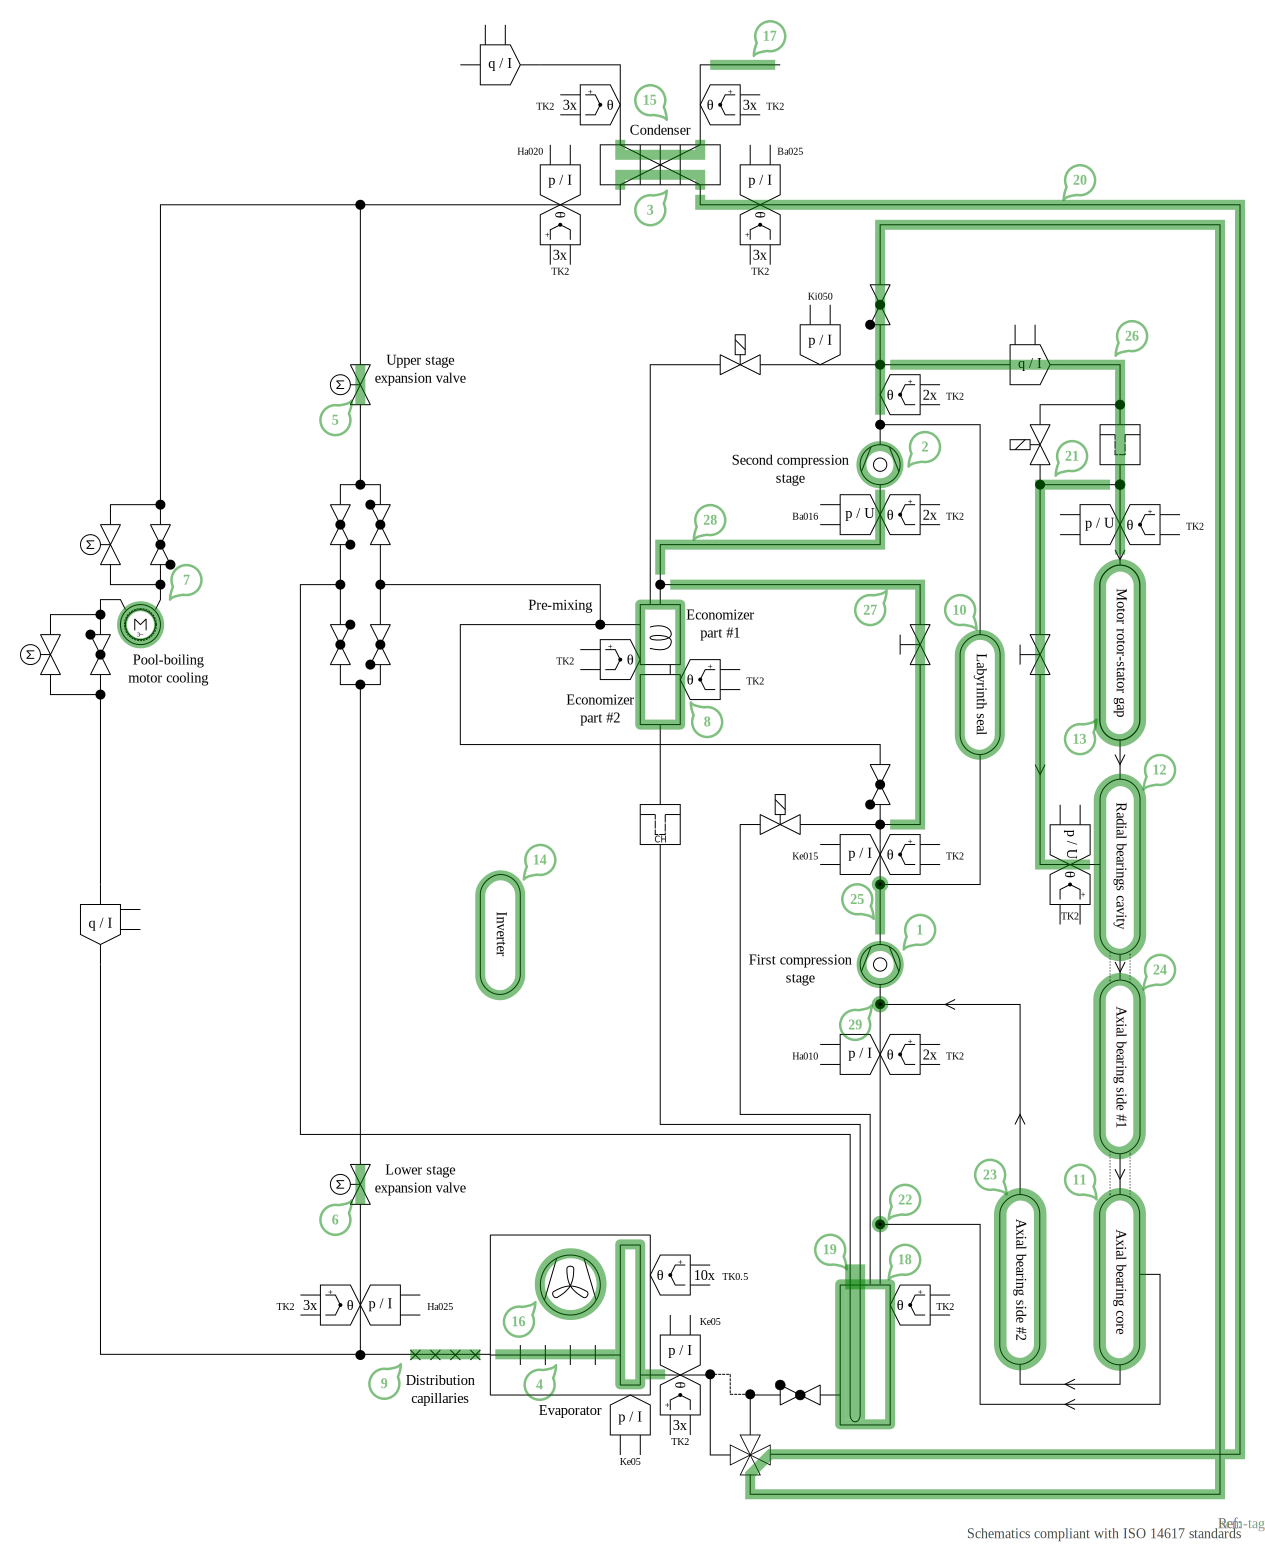
\includegraphics[width=1\textwidth]{awp-layout}
  \caption[AWP layout with components numbers]
  {AWP layout, with components numbers}
  \label{fig:awp-layout-model-numbers}
\end{figure}

\begin{figure}[htbp]
  \centering
  \includegraphics[width=0.65\textwidth]{awp-exp-analysis-model}
  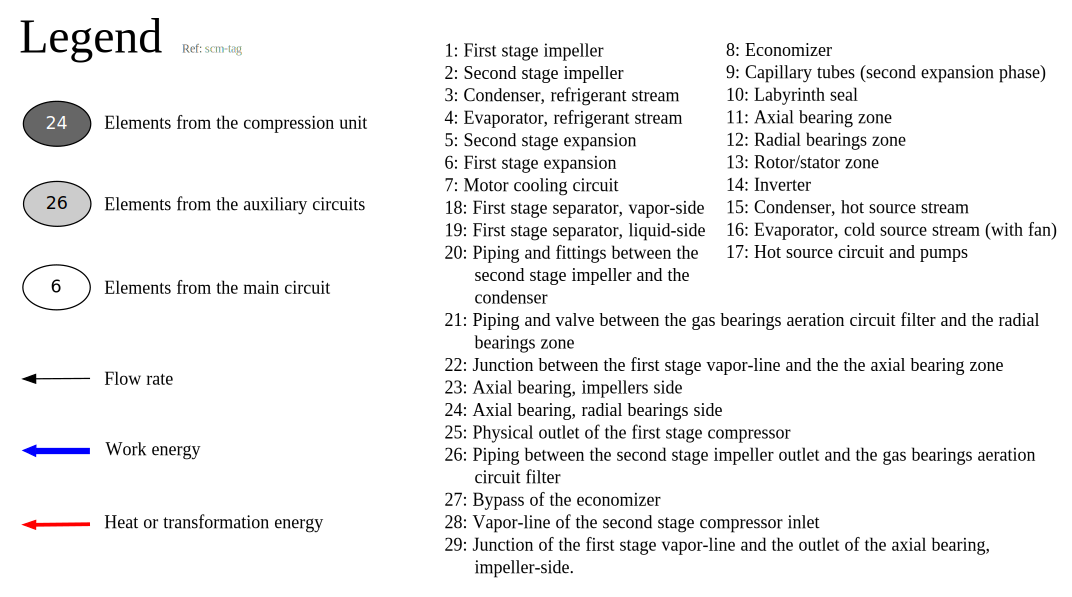
\includegraphics[width=0.95\textwidth]{awp-exp-analysis-model-legend}
  \caption[AWP model]{AWP model}
  \label{fig:awp-exp-analysis-model}
\end{figure}


This section only displays the details of some of the \AWP{} main
components. The level of detail given in this section corresponds to
the mandatory level needed to understand the contents of
\crefrange{sec:awp-model}{sec:awp-perfs}. \Cref{chap:awp-components}
extends those details and displays information about the components
that have not been described here, or only partially.

\subsection{Compression unit}
\label{sec:awp-cp-unit}

The compressor is a main component of vapor compression heat pump
cycles and has two main functions:

\begin{itemize}
\item Compress the refrigerant vapor from the evaporator so that the
  desired temperature and pressure can be maintained in the evaporator
  \citep[p.\,109]{dincer-kanoglu-2010a}.
\item Increase the pressure of the refrigerant vapor through the
  process of compression, and simultaneously increase the temperature
  of the refrigerant vapor \citep[p.\,109]{dincer-kanoglu-2010a} in
  order to meet the required condensation conditions \citep{rapin-desmons-2011a}.
\end{itemize}

Those two functions can not be fulfilled without the use of expansion
devices on liquid lines. The compressor role in the heat pump
prototype studied here is performed by a compression unit containing
the two compression stages, rotating at the same speed. The prototype
compression unit tested in the \AWP{} was the \textit{cp105}
compression unit, from the \textit{evo4} design family. Compression
units from \textit{evo1} and \textit{evo2} families have almost not
been tested in the \BWP{} or the \AWP{}, as those units were not ready
for heat pump integration. Compression units from the \textit{evo4}
family were the first decently working prototypes that have been
available for tests\footnotep{More details about the compression unit
  history is given in \cref{sec:bwp-cp-unit}.}. They started to be
available during Spring 2012. One unit from the \textit{evo4} family,
the \textit{cp105} unit has been tested in the \AWP{} in May 2012. The
datasets presented in this work have been generated during that
period. An other unit of this family, \textit{cp101}, assembled before
the \textit{cp105} unit, has been tested later in the \BWP{}, in
October 2013. Because of confidentiality issues, the details of the
design of the units or the differences between the different
compression unit design families can not be exposed in this work and
are only partially known by the author himself. However, the structure
of the \textit{cp105} unit and its connections with the heat pump main
and auxiliary circuits are described in
\cref{fig:cp105-struct-awp}. The main differences with the version
tested in the \BWP{} are:

\begin{description}
\item[Motor cooling configuration] The motor cooling configuration
  tested on the \textit{cp105} unit was a pool-boiling
  configuration. In the \BWP{}, the motor was cooled down with a
  flow-boiling configuration\footnotep{Details about the motor cooling
    parts are given in \cref{sec:awp-motor-cooling-details}
    page~\pageref{sec:awp-motor-cooling-details}.}.
\item[Gas bearings aeration inlets/outlets configuration] The gas
  bearings aeration circuit injects cold gas at the back of the
  compression unit (inlet \#1), after the motor (component
  \#13\footnotep{For components description and numbering, see
    \cref{fig:awp-layout-model-numbers,fig:awp-exp-analysis-model},
    page~\pageref{fig:awp-layout-model-numbers}
    and~\pageref{fig:awp-exp-analysis-model}.}), and in the radial gas
  bearings cavity (component \#12)
  (inlet \#2). The gas flows through the gap between the stator and
  the rotor, cooling down the two parts, and evacuating windage
  losses. This gas flow is mixed with the flow coming from the second
  inlet and leaves through the axial bearing of the motor
  side (component \#24) towards the
  outlet of the gas circuits, which is the middle of the set of axial
  bearings (component \#11). A share of
  this flow leaves by entering the axial bearing of the impeller
  side (component \#23)\footnotep{This
    gas path was not the one expected and this issue is discussed with
    further details in \cpref{sec:axial-is-reversed}.}.
\end{description}


\begin{figure}[htbp]
  \centering
  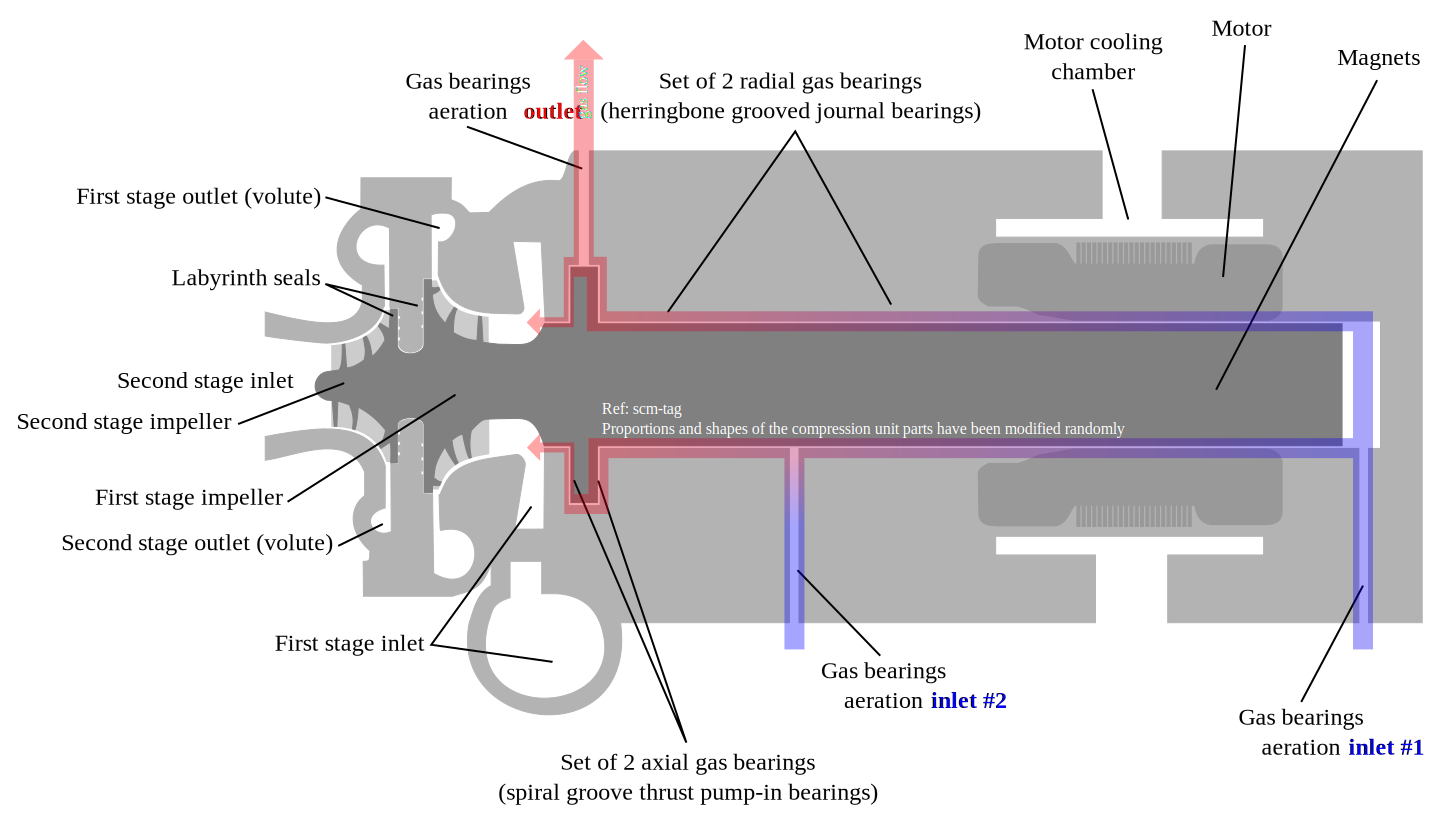
\includegraphics[width=\linewidth]{cp105-wheel-details-awp}
  \caption[Structure of the compressor unit with the AWP gas bearings
  aeration circuit I/O layout]{Structure of the twin-stage compressor
    unit with the AWP gas bearings aeration circuit inlets/outlets
    layout. Those inlets/outlets are different on the BWP, as
    illustrated in \cref{fig:cp101-struct-bwp}, page
    \pageref{fig:cp101-struct-bwp}.  Differences are stressed with a
    bold font.}
  \label{fig:cp105-struct-awp}
\end{figure}

\begin{figure}[htbp]
  \centering
  \subfloat[View of AWP]
  {\label{fig:awp-in-climate-chamber}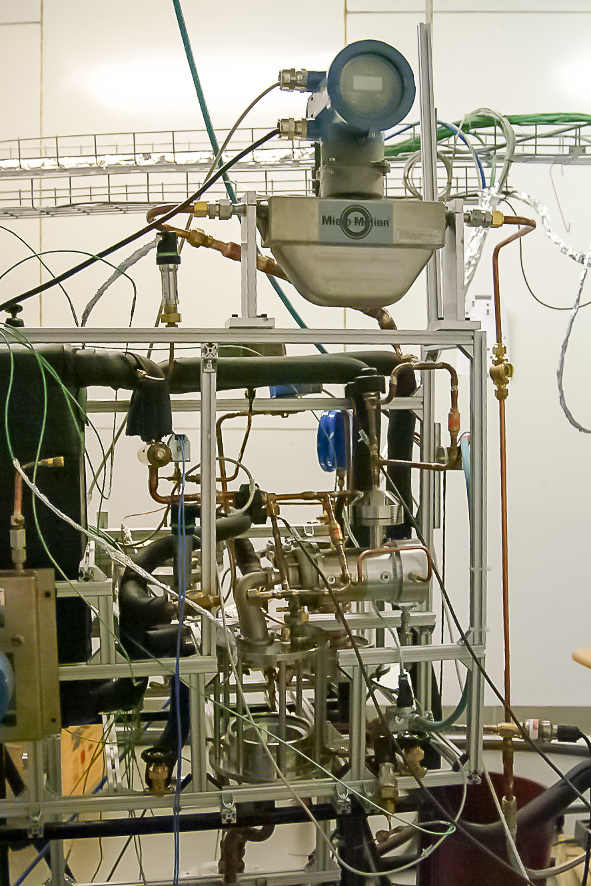
\includegraphics[height=10cm]{DSCF0217}}
  \hspace{1em}
  \subfloat[View of the evaporator]
  {\label{fig:awp-ev}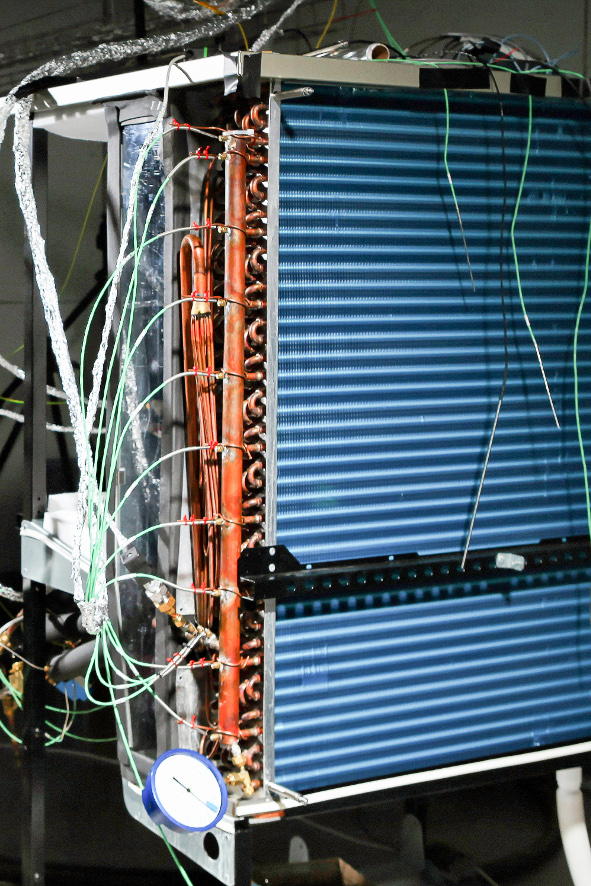
\includegraphics[height=10cm]{awp-ev}}
  \caption[Views of the AWP]{Views of the AWP. The extension of the
    economizer (component \#8) is located below its main part. The
    pipe connecting the two parts is visible at the bottom of the
    picture. Extra flow meters (one can be seen in
    \cref{fig:awp-in-climate-chamber}) have been added outside the
    original device housing, in order to understand the behavior of
    the prototype and characterize the system. The evaporator
    (\cref{fig:awp-ev}) is instrumented with a thermocouple per
    channel.}
  \label{fig:awp-views-in-climate-chamber}
\end{figure}

\begin{figure}[htbp]
  \centering
  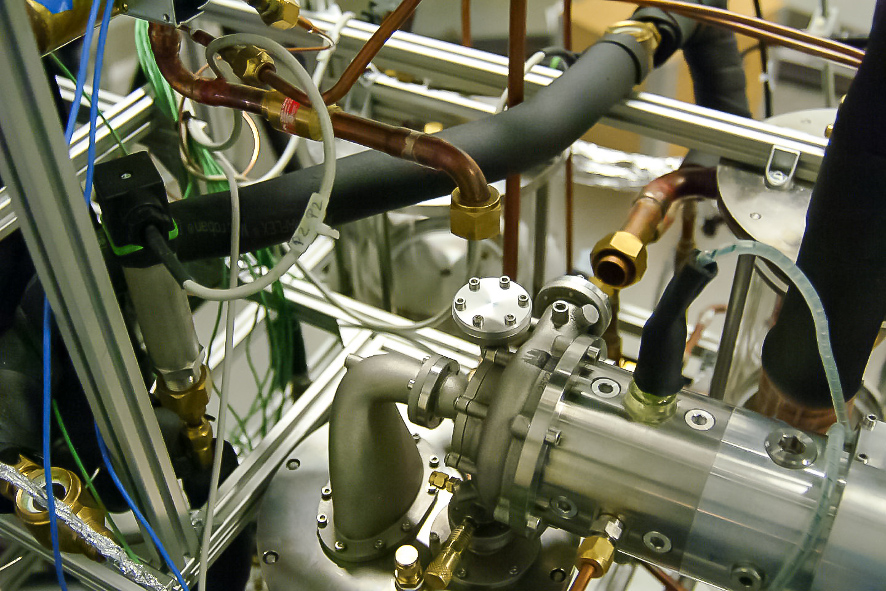
\includegraphics[width=12cm]{DSCF0215}
  \caption{Compression unit \textit{cp105}, being mounted in the AWP}
  \label{fig:cp105-being-mounted-in-awp}
\end{figure}


\subsection{Compression stage bypass systems}
\label{sec:awp-bypass}

Bypass circuits are mandatory auxiliary circuits in heat pumps
integrating the radial compression units. In the \AWP{}, each
compression stage is equipped with a bypass circuit consisting of a
manual needle valve, used to set the characteristics of the bypass,
and a solenoid valve for rapid bypass activation. This
solution had been chosen for cost-related reasons, and because the
crucial role of the bypass circuits dynamic response had not been
identified at the time. Fast electric needle valves are quite big and
expensive and were not appropriate if referred to the prototype
specification defined in \cref{sec:awp-specs}. The \BWP{} has been
equipped with such a valve for its bypass system, which is quite
different from the one used in the \AWP{}, as illustrated in
\cpref{fig:bypass-schematics}. The \BWP{} bypass system bypasses both
compression stages together, as described in
\cpref{sec:bwp-bypass-system} while the \AWP{} bypass system bypasses
each compression stage independently. However, being able to open or
close the bypass circuits independently in the \AWP{} does not make
them independent, as illustrated in
\cref{fig:awp-bypass-simple-layout}.


\subsection{Economizer}
\label{sec:awp-eco}

The \AWP{} is equipped with glass-made separator and economizer to
allow an easier monitoring and understanding of the refrigerant
distribution. This configuration allows for instance to see the
topology of the flow or to see if droplets appear at critical
locations. To prevent liquid management issues during the tests at the
laboratory, the inlet separator and the economizer should be able to
contain a good share of the refrigerant charge. When the heat pump
cycle is reversed for cooling or defrosting mode, part of the
refrigerant charge is likely to flow from the condenser to the
evaporator in a short time, due to the pressure difference between
those two components. This volume of liquid is likely to arrive in the
first stage inlet separator, consequently. In normal operation, the
liquid content of each heat exchanger is determined by its flow
conditions and characteristics (pinch diagram and flow pattern maps,
notably). The charge which is not contained in the heat exchangers at
a given time is collected in the economizer, which has to be able to
contain this charge while ensuring its liquid/gas separation function
properly. In order to decrease the impact of control mistakes during
the experiments, the volumes of the first stage compressor inlet
separator and of the economizer have been increased by a factor two by
duplicating them and by mounting the duplicates and the main parts
together\footnotep{See \cref{sec:awp-eco-appendix}
  page~\pageref{sec:awp-eco-appendix} for details.} in the prototype
(as illustrated in \cref{fig:awp-3d-layout}).

Gas/liquid separation issues were encountered in the economizer during
the experiments, so the design of the gas/liquid separation parts in
the economizer have evolved significantly during the experimental
investigation. The successive versions are detailed in
\cref{fig:awp-eco-gas-liq-sep-1-to-5}. The data presented in this
thesis work has been generated with the \AWP{} equipped with version
\#4 (before May 25\th{}, 2012) and version \#5 (after May 25\th{},
2012) of the economizer. An other action taken to solve the separation
issue was to move the second part of the economizer below the main
part, in order to increase the distance between the liquid level and
the second stage compressor inlet. The two components were connected
with a 20cm-long 3/4-inch pipe.

\begin{figure}[htbp]
  \centering \subfloat[Gas/liquid separation, version \#1 to \#4]
  {\label{fig:awp-eco-gas-liq-sep-1-to-4}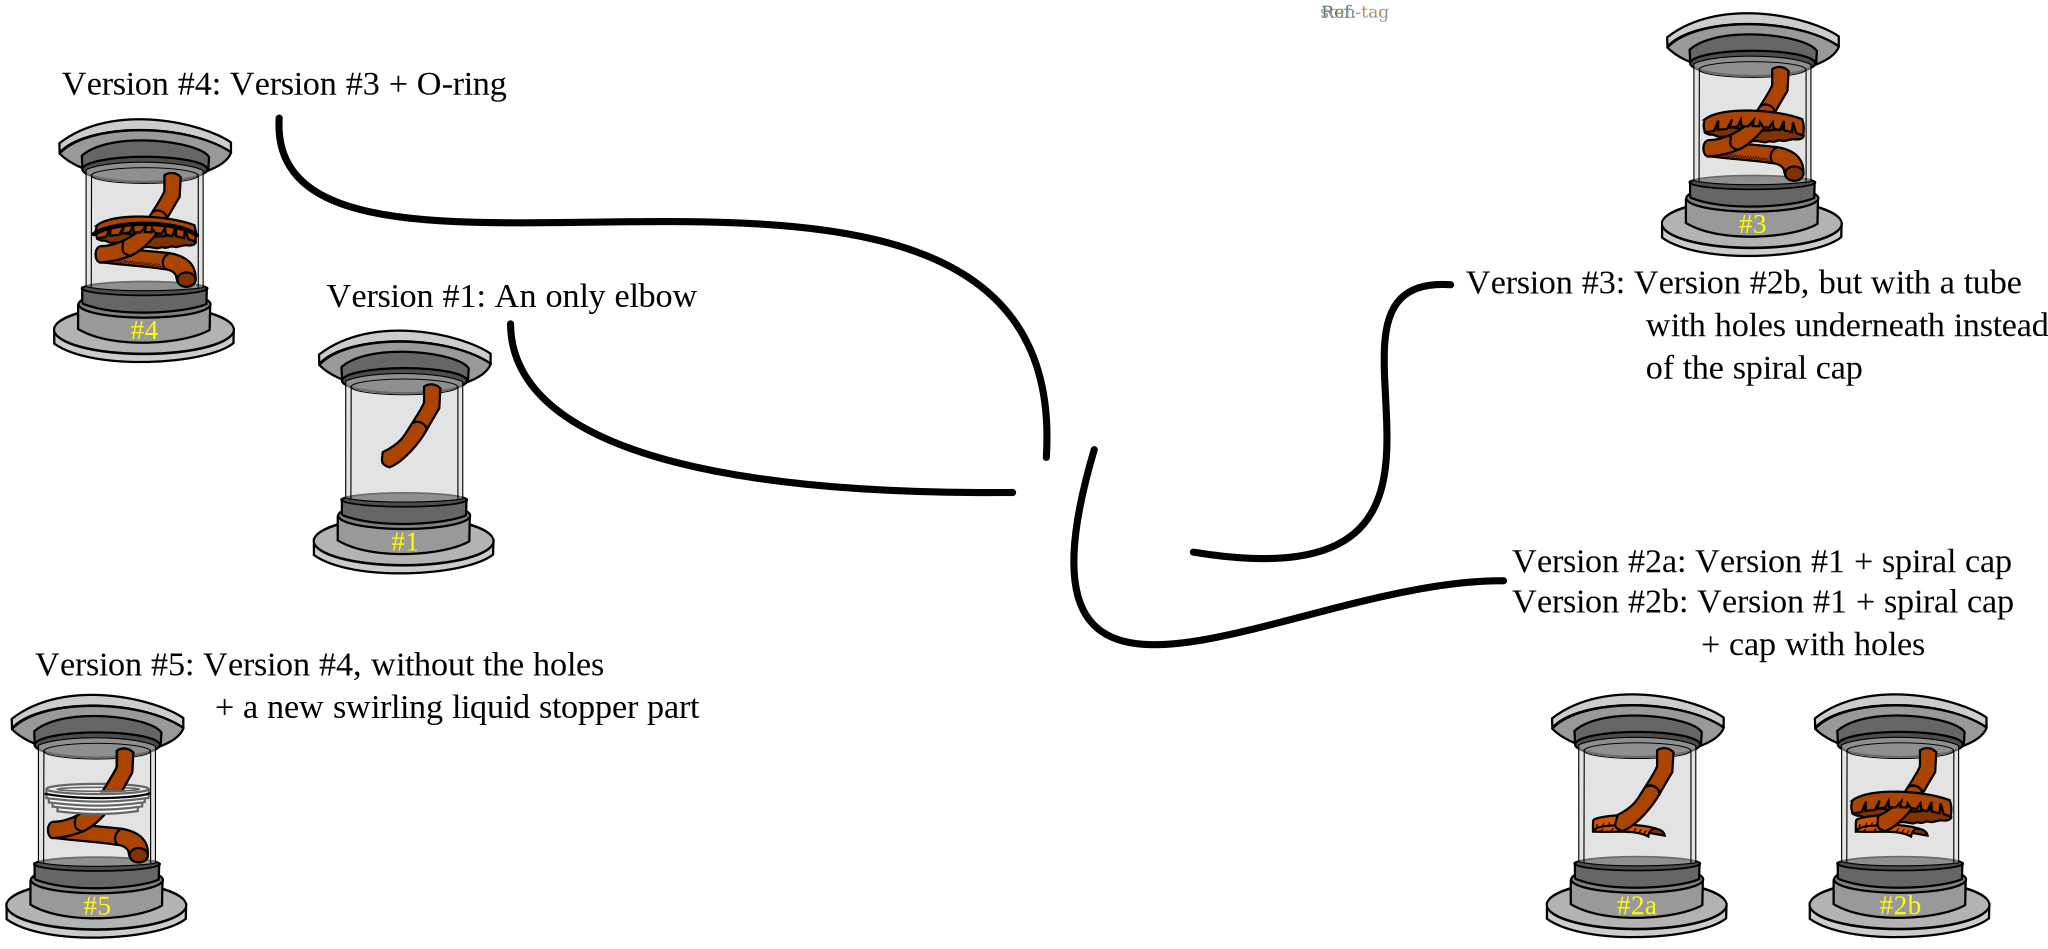
\includegraphics[width=\linewidth]{awp-eco-gas-liquid-sep-v1-to-v4}}
  \\\vspace{4em}
  \subfloat[Version \#5 (big central hole, with a seal and shapes to
  send the liquid back down the economizer on the sides)]
  {\label{fig:awp-eco-gas-liq-sep-5}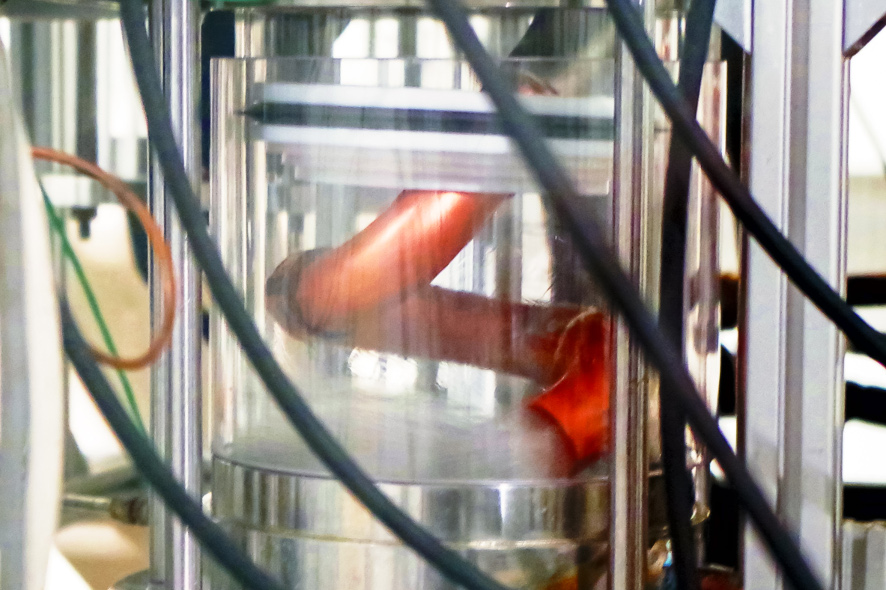
\includegraphics[width=12cm]{DSCF0172-mod}}
  \caption{AWP economizer version \#1 to \#5.}
  \label{fig:awp-eco-gas-liq-sep-1-to-5}
\end{figure}

\begin{figure}[htbp]
  \centering
  \begin{minipage}[r]{.49\linewidth}
    \begin{flushright}
      \subfloat[View \#1 ]{\label{fig:awp_assembly_1}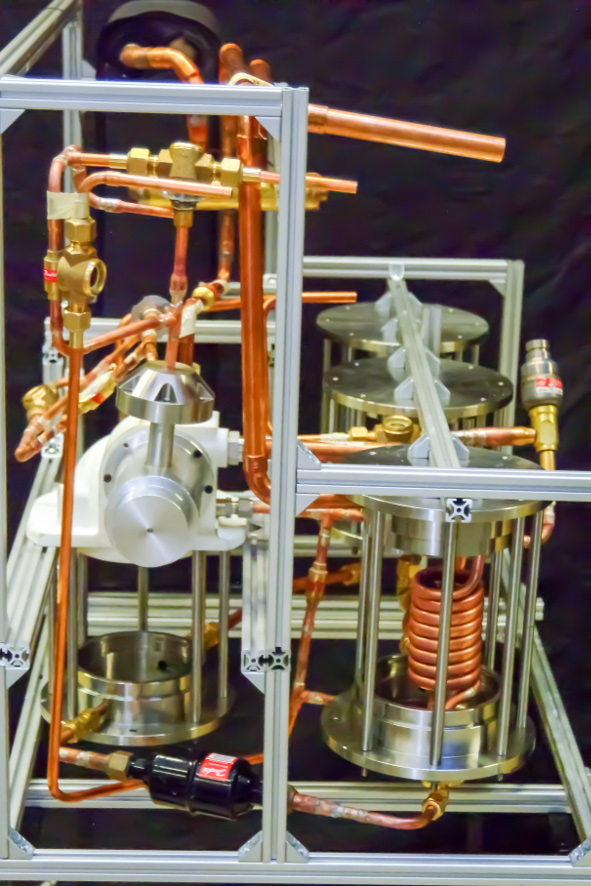
\includegraphics[height=11cm]{DSCF0016-mod}}
    \end{flushright}
  \end{minipage} \hfill
  \begin{minipage}[l]{.49\linewidth}
    \begin{flushleft}
      \subfloat[View \#2]{\label{fig:awp_assembly_2}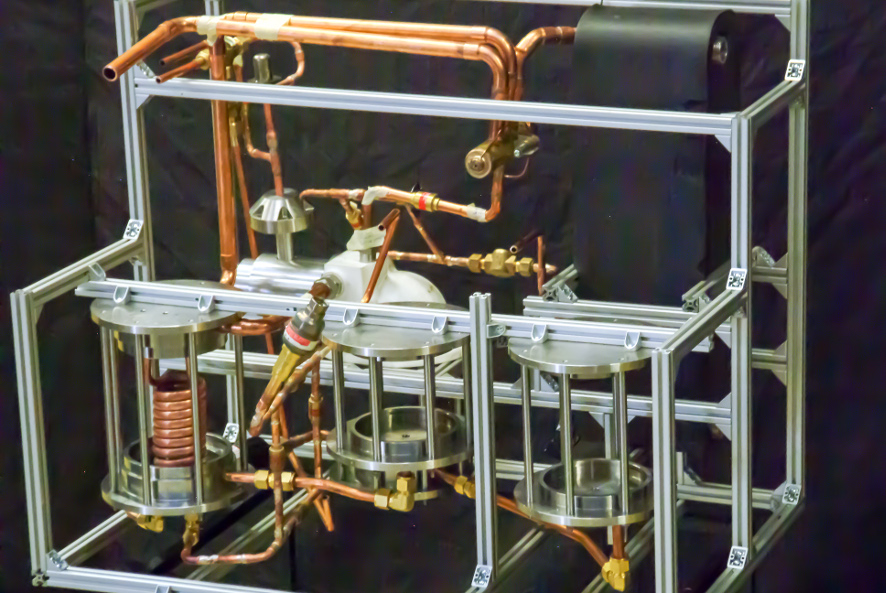
\includegraphics[height=5.07cm]{DSCF0017-mod}} \\
      \subfloat[View \#3]{\label{fig:awp_assembly_3}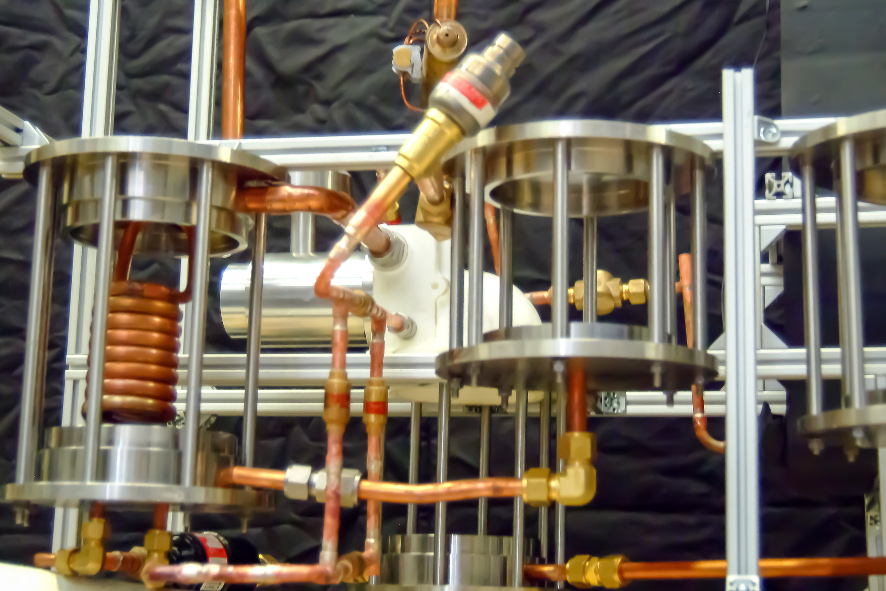
\includegraphics[height=5.07cm]{DSCF0002-mod}}
    \end{flushleft}
  \end{minipage}
  \caption{AWP assembly}
  \label{fig:awp_assembly}
\end{figure}

\begin{figure}[htbp]
  \centering \subfloat[Very low flow rate]
  {\label{fig:awp_eco_vlow_mf}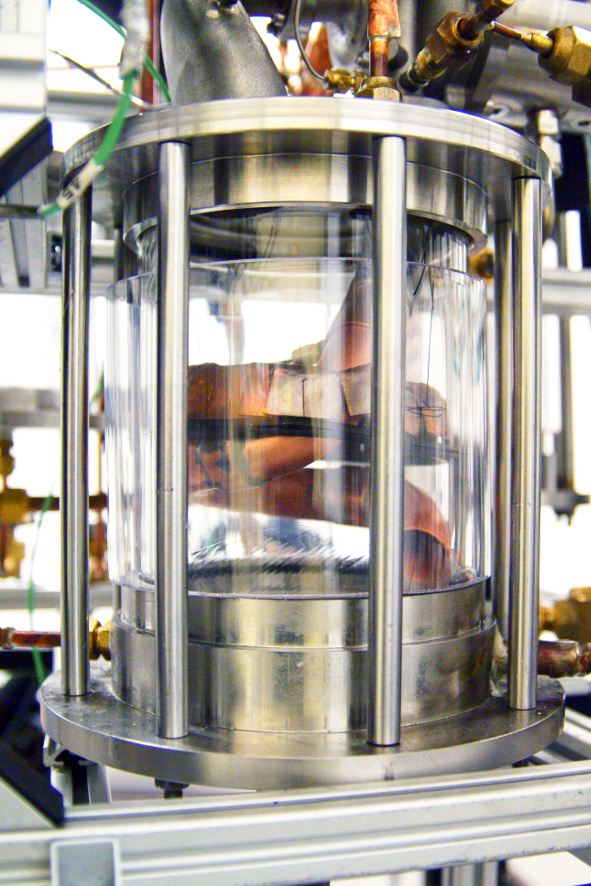
\includegraphics[width=0.45\linewidth]{DSCF0093-mod}}
  \hspace{1em} \subfloat[Liquid flowing up]
  {\label{fig:awp_eco_flow_up}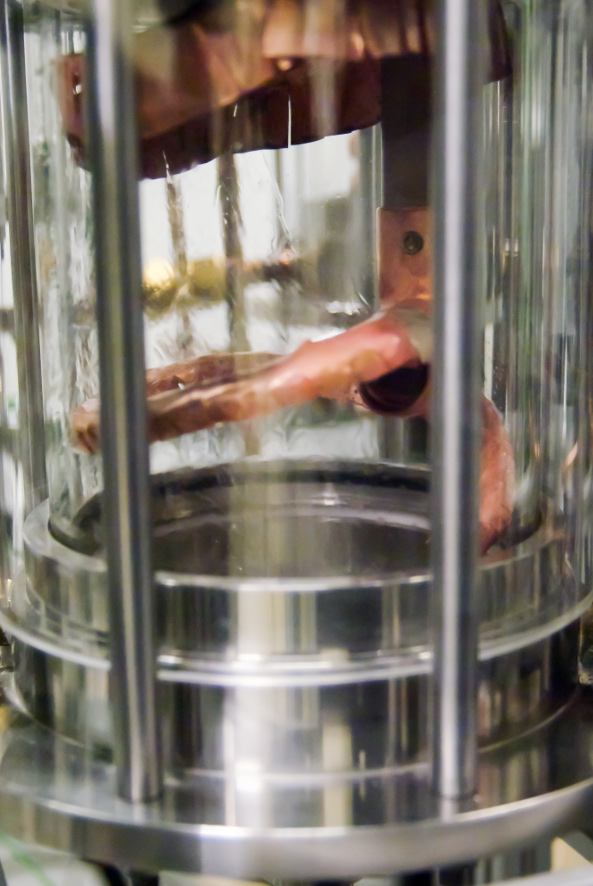
\includegraphics[width=0.45\linewidth]{DSCF0098_120krpm}}
  \\
  \subfloat[Low flow rate]
  {\label{fig:awp_eco_low_mf}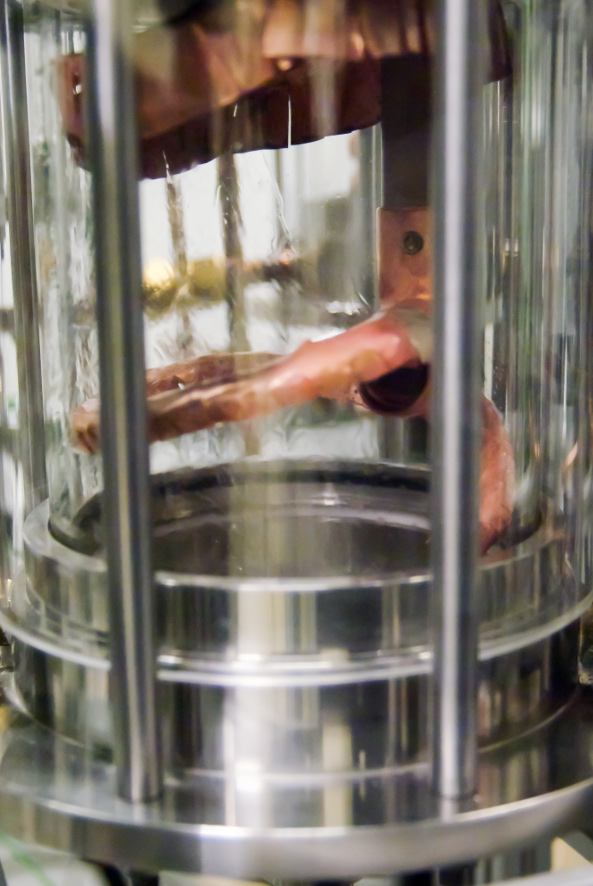
\includegraphics[height=70mm]{DSCF0098_120krpm}}
  \hspace{1em} \subfloat[Moderate flow rate]
  {\label{fig:awp_eco_mid_mf}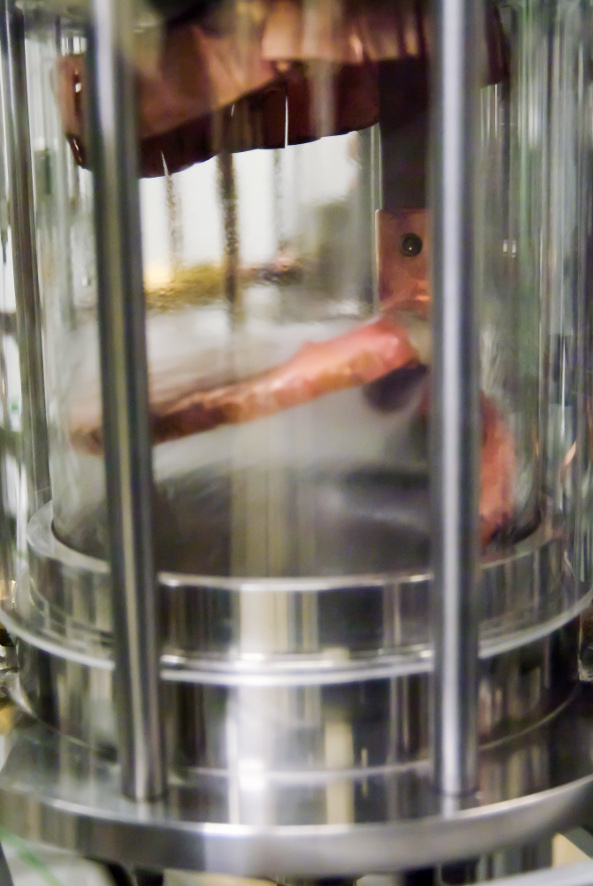
\includegraphics[height=70mm]{DSCF0095_120krpm}}
  \hspace{1em} \subfloat[High flow rate]
  {\label{fig:awp_eco_high_mf}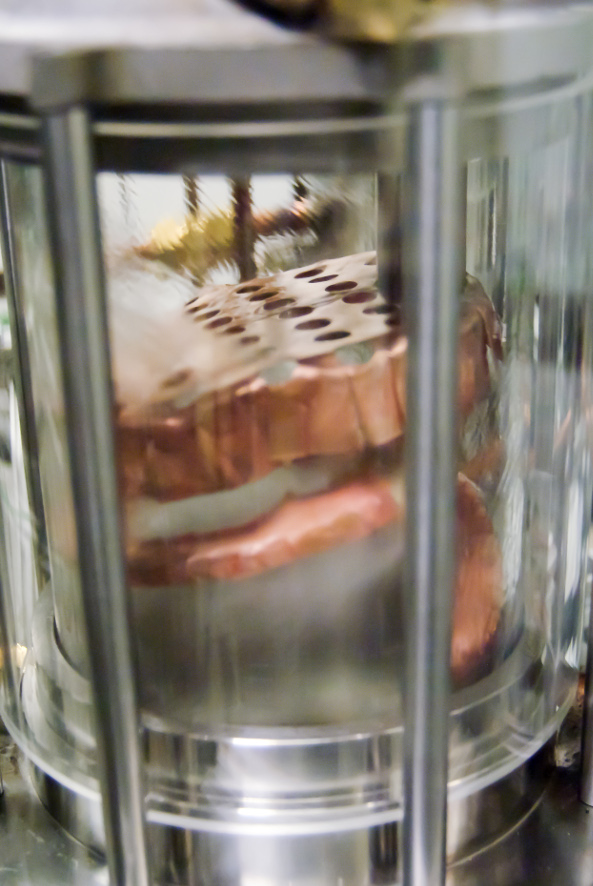
\includegraphics[height=70mm]{DSCF0070_110krpm}}
  \caption[Gas/liquid stream patterns with qualitative flow
  velocities]{Gas/liquid stream patterns with qualitative flow
    velocities. The gas/liquid separation assemblies used in this
    illustration are assemblies version \#2a, \#2b, and \#4.}
  \label{fig:awp-eco-flow-rates}
\end{figure}

\subsection{Evaporator}
\label{sec:awp-ev}

The evaporator of the \AWP{} is pictured on \cref{fig:awp-ev}. Its
detailed geometry and characteristics are available in
\cref{awp-ev-details}. The air ducting of the heat pump housing used
as a base for the \AWP{} design occurred to be designed with
compactness in mind and has not been designed for optimum air streams
or noise reduction. The goal of the designers was clearly to design a
heat pump unit able to go through the width of a conventional domestic
doorway. As a result of those design choices, the air stream
distribution in the air ducting was far from being satisfactory, as
detailed in \cref{sec:awp-issue-reducing-oh}. In order to try to
compensate for this issue, a plate drilled with holes in front of the
evaporator channels which had the lowest degree of superheat at their
outlets has been added at the inlet of the air ducting. This plate and
its influence on the superheating profile along the height of the
evaporator are detailed in \cref{sec:awp-issue-reducing-oh}.

\subsection{4-way valve}
\label{sec:awp-4way}

A 4-way reversing valve is included in the heat pump circuits in order
to switch between heating-mode, cooling-mode, and defrosting-mode. It
can be seen in \cref{fig:awp-4way-valve-in-circuits}. Such a valve
allows the condenser and evaporator to exchange their role in the heat
pump cycle in order to defrost the evaporator during the heating
period, or for space cooling application. The flow of the refrigerant
in the exchangers is reversed and the roles of the exchangers are
exchanged. The valve is mounted on the suction line of the first
compression stage and the discharge line of the second compression
stage. The slide assembly inside the valve can translate to connect
the appropriate ports for the desired operation mode. It generates
additional pressure drops, a leakage flow and a heat exchange between
the discharge and the suction ports
\citep[p.\,4]{bertsch-hubacher-2002a}. This leakage has been measured
by \citet[p.\,39]{bertsch-hubacher-2002a} for a type of 4-way valve
very similar to the one used in the \AWP{} and have been measured
between 1 and 3 \si{\milli\gram\per\second\per\bar} with R134a. The
valve used in \AWP{} has been cleaned in order to remove any lubricant
contained within the valve\footnotep{The application here must be
  oil-free, as detailed in \cpref{sec:awp-issue-oil+corrosion}.},
which has certainly contributed to increase the leakage between the
suction and discharge ports, as the oil acts also as a sealant. This
leakage is neglected in the frame of this study. The 4-way valve in
the \AWP{} is the valve that was already present in the industrial
partner heat pump delivered to EPFL.

\begin{figure}[htbp]
  \centering
  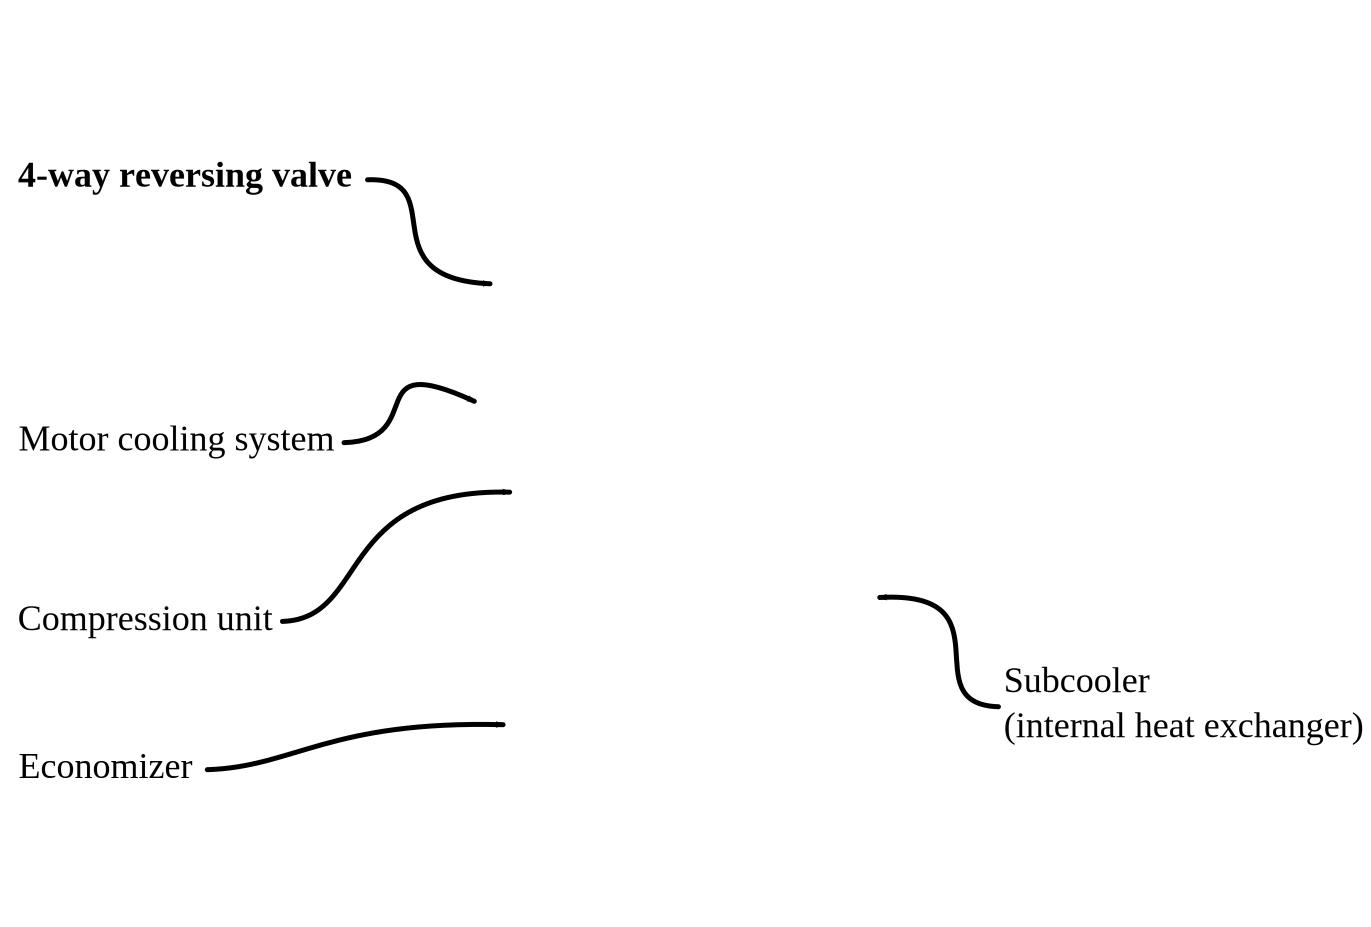
\includegraphics[width=15cm]{awp-4way-valve}
  \caption{View of the 4-way reversing valve in the heat pump circuits}
  \label{fig:awp-4way-valve-in-circuits}
\end{figure}


\section{Modeling}
\label{sec:awp-model}

The model proposed is based on the areas or physical elements of
interest in the \AWP{}. \Cref{fig:awp-layout-model-numbers} presents
the \AWP{} layout and \cref{fig:awp-exp-analysis-model} presents the
model itself. The set of equations deduced from analysis of the model
in \cref{fig:awp-exp-analysis-model} is detailed in
\cref{chap:awp-eqn}.

Following the procedure described in \cref{sec:methodo-models}, the
model is built with 29 components; 11 of them describe the compression
unit itself.

\section{Prototype performance}
\label{sec:awp-perfs}

A stable\footnotep{An OP is considered
  stable if it qualifies to defined conditions. See
  \cref{sec:stable-op} page~\pageref{sec:stable-op} for details.} \OP{} insures that the experimental setup is in a steady
state, which allows to use the modeling technique presented in
\cpref{sec:methodo-models}. Indeed, one of the main assumptions of
this modeling technique is that the system being analyzed is in a
steady state. The maximum rotor speed reached with the compressor unit is 180
krpm, which is the maximum rotor speed of the compression unit, by
design. The maximum rotor speed reached for a stable \OP{} is 171
krpm.

The first and the second \OP{}, A-6.8/W31.3 and A-7.0/W32.3 are two
similar \OP{}\footnotep{The first and second OP are detailed
  respectively in \cpref{sec:awp-exp-details-A-6.8/W31.3} and
  \cpref{sec:awp-exp-details-A-7.0/W32.3}.}, regarding temperature
levels. One has been measured with the 4-way reversing valve, one has
been measured without. The consequence of this modification of the
heat pump circuits is detailed in \cref{sec:awp-issue-4way}. The third
\OP{}\footnotep{The third OP is detailed in
  \cpref{sec:awp-exp-details-A-7.0/W35.6}.}, A-7.0/W35.6, yields the
highest temperature lift between the sources. It allows a comparison
of the \AWP{} with industrial products currently on the market, since
A-7/W35 is a common \OP{} for heat pump ranking and
comparison \citep{EN-14511-3}. The next three \OP{}\footnotep{Those 3
  OP are detailed respectively in
  \cpref{sec:awp-exp-details-A-0.5/W20.7},
  \cpref{sec:awp-exp-details-A-3.1/W29.5}, and
  \cpref{sec:awp-exp-details-A-6.6/W22.1}.}, A-0.5/W20.7, A-3.1/W29.5,
and A-6.6/W22.1, illustrate the gas temperature profile behavior
inside the compression unit, with the increase of the rotation
speed. This issue is documented in \cref{sec:awp-laby-hot-gas}.

\Cref{tab:awp-performances-summary} summarizes the main performance
indicators for the 6 stable \OP{}. The inverter is considered to be
inside the internal frontier in the model presented
\cref{fig:awp-exp-analysis-model}, since its efficiency is not
properly known. Indeed, it could be measured only once, with the
compressor unit running at 120 krpm, as the laboratory was not
equipped to perform high frequency three-phase power measurements on a
regular basis. Consequently, this measured efficiency of 85\% is
considered constant in this thesis work. The \COP{} is consequently
defined as expressed in \cpref{eq:COPh}, and considers the inverter to
be part of the internal system. \COP{}, as defined in \cref{eq:COPh},
does not take into account the pumps or the fan energy consumption
for the auxiliary fluids. The experimental results show differences of
temperature between the sources from 28.7 to 42.6 degrees and \COP{}
ranges from 2.19 to 4.02 in the stable \OP{} reached. The overall
exergy efficiencies, defined in \cpref{eq:eta_heatpump}, range from
26.3\% to 32.6\%. Those exergy efficiencies are considered low, as
they could have reached 30 to 40\% with better heat exchangers,
notably with a better evaporator\footnotep{The evaporator exergy
  efficiency $\eta_{ev}$, in the OP detailed in
  \cref{tab:awp-performances-summary}, ranges from 17\% to 34\% (see
  \cpref{sec:awp-issue-reducing-oh}) and is calculated with
  \cpref{eq:eta_ev_awp}. The subcooler exergy efficiency $\eta_{sc}$
  ranges from 0.4\% to 3\% (see \cpref{sec:awp-low-etaII-sc}) and is
  calculated with \cpref{eq:eta_sc}.}, improved
insulation\footnotep{The prototype was only partially insulated, as
  this can be seen on \cref{fig:awp-in-climate-chamber}
  page~\pageref{fig:awp-in-climate-chamber}.}, better control of the
auxiliary circuits\footnotep{The motor cooling flow was often not
  appropriate, as detailed in \cref{sec:awp-issue-motor-cooling}
  page~\pageref{sec:awp-issue-motor-cooling}, and the gas bearings
  aeration flow was not easy to set at a chosen value, as described in
  \cref{sec:awp-low-etaII-sc} page~\pageref{sec:awp-low-etaII-sc}.},
and better control of the subcooling and superheating
values\footnotep{Those values were not easily controlled, as explained
  in \cref{sec:awp-issue-control,sec:awp-issue-reducing-oh},
  page~\pageref{sec:awp-issue-control}.}. The most interesting \OP{}
is the \OP{} A-7.0/W35.6\footnotep{More details about this specific OP
  are given in \cref{sec:awp-exp-details-A-7.0/W35.6}
  page~\pageref{sec:awp-exp-details-A-7.0/W35.6}.}, which allows to
compare the \AWP{} performance with industrial products performance
using conventional technology, even if the comparison is not very
accurate, as the prototype tests were not strictly performed in the
conditions imposed by the standards relative to performance
measurement of heat pumps with electrically driven compressors for
space heating \& cooling
applications \citep{EN-14511-1,EN-14511-2,EN-14511-3,EN-14511-4,EN-14825}
\footnotep{Acoustic measurements conditions are detailed in other
  standards \citep{EN-12102,EN-ISO-9614-1}.}. Notably, the fan and pump
electrical powers were not taken in account \citep[sec.\,4.1.4 and
4.1.6]{EN-14511-3}, the condenser water temperature difference was of
\num{6.84}\si{\kelvin}, instead of
5\si{\kelvin} \citep[tab.\,12]{EN-14511-2}\footnotep{The standard
  condenser inlet/outlet water for this OP are 30\si{\degreeCelsius}
  at the inlet and 35\si{\degreeCelsius} at the outlet.}, and the
condenser inlet temperature was not exactly at
\num{35.0}\si{\degreeCelsius}, but at
\num{35.6}\si{\degreeCelsius}. Nonetheless, it appears that the \AWP{}
performs close to the devices currently on the market, as it can be
seen in \cref{tab:awp-indus-products-comparison}. Indeed, the \AWP{}
performance is a little lower than the devices it compares with
(\COP{} is 0.2 to 0.5 points lower). Reaching this level of
performance is encouraging, since even this first working prototype,
far from being a complete optimized industrial version, already ranks
close to the models currently on the market. In addition to the
drawbacks mentioned above, the prototype topology was burst around in
order to include measurement capabilities, creating pressure drop. As
illustrated in \cref{fig:awp-A-7.0/W35.6-sankey-energy}, about 6\% of
the energy was dissipated in the environment during this experiment
A-7.0/W35.6. Those 6\% include the heat losses of the
inverter (component \#14). This heat
energy could be also recovered by the thermodynamic cycle, for
instance, as it is already the case for the motor heat
losses. Moreover, the control issues detailed in
\cref{sec:awp-control-issues} have also a negative influence on the
prototype performance. As a consequence, even if they are
comparatively low, the performance reached with this first working
prototype is considered very promising and constitutes a breakthrough
in the domain.

\begin{figure}[htbp]
  \centering
  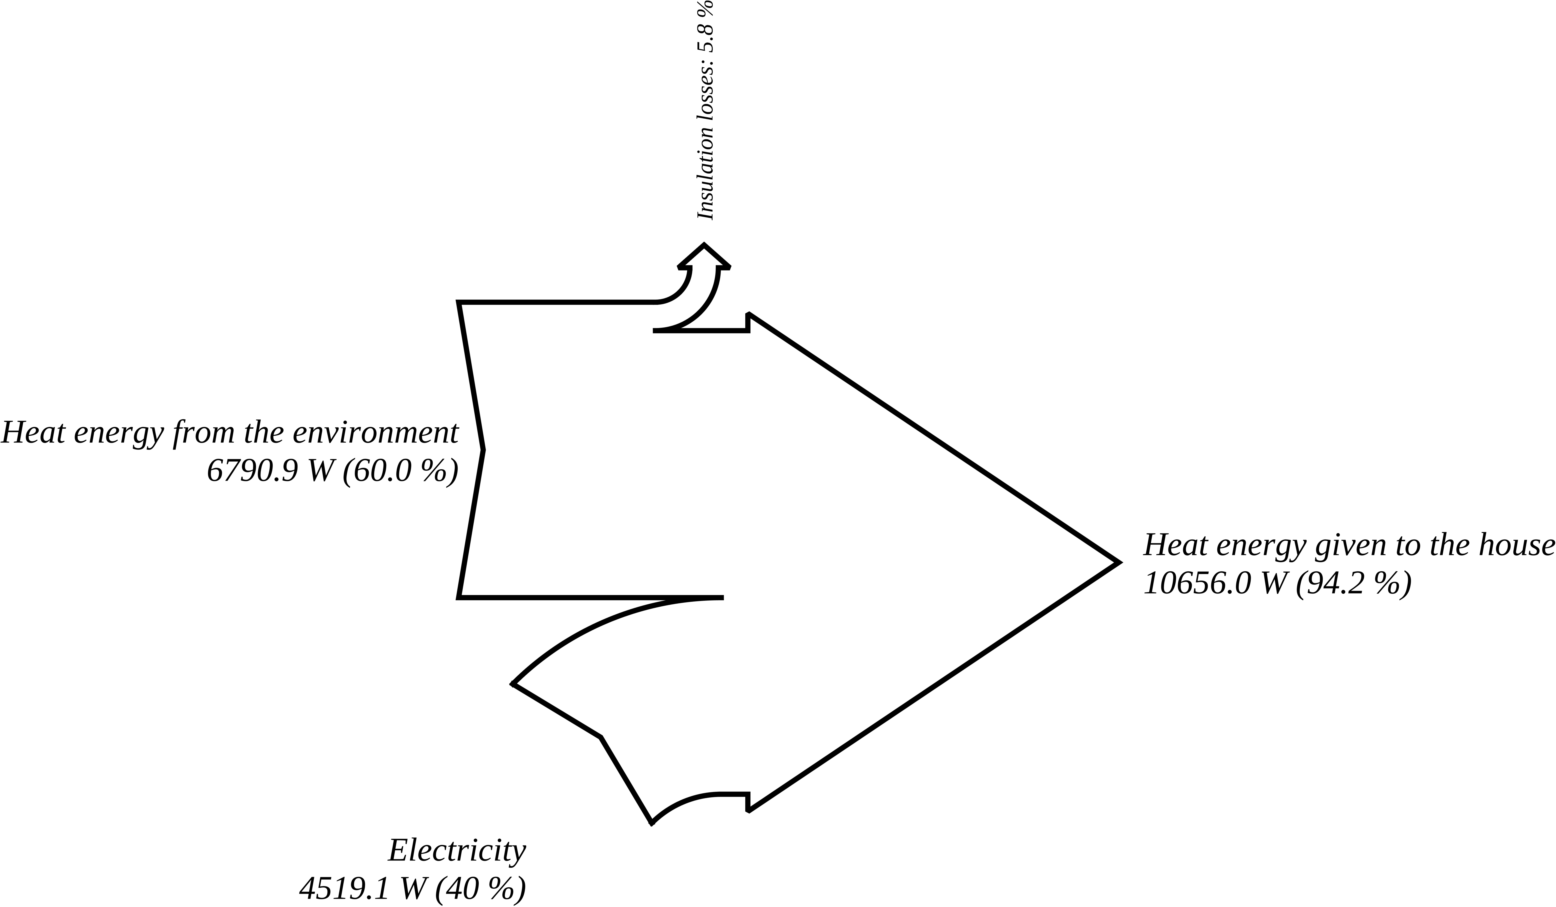
\includegraphics[width=1\textwidth]{awp-energy-sankey-awp-20120525-150822-151122}
  \caption{A-7.0/W35.6 - Sankey diagram for heat pump energy balance (internal frontier)}
  \label{fig:awp-A-7.0/W35.6-sankey-energy}
\end{figure}


\begin{table}[htbp]
  \begin{center}
    \footnotesize
    \begin{tabular}{lccccccc}
\toprule
\OP{} \# & & \#1 & \#2 & \#3 & \#4 & \#5 & \#6 \\
\OP{} & & A-6.8/W31.3 & A-7.0/W32.3 & A-7.0/W35.6 & A-0.5/W20.7 & A-3.1/W29.5 & A-6.6/W22.1 \\
Data & & \cref{sec:awp-exp-details-A-6.8/W31.3} & \cref{sec:awp-exp-details-A-7.0/W32.3} & \cref{sec:awp-exp-details-A-7.0/W35.6} & \cref{sec:awp-exp-details-A-0.5/W20.7} & \cref{sec:awp-exp-details-A-3.1/W29.5} & \cref{sec:awp-exp-details-A-6.6/W22.1} \\
Speed & & 170 krpm & 160 krpm & 171 krpm & 130 krpm & 153 krpm & 160 krpm \\
\midrule
 $ \epsilon_h $ & -  & $ \num{2.19} \pm \num{0.04} $ & $ \num{2.69} \pm \num{0.03} $ & $ \num{2.36} \pm \num{0.03} $ & $ \num{4.02} \pm \num{0.06} $ & $ \num{3.10} \pm \num{0.04} $ & $ \num{2.67} \pm \num{0.05} $ \\
 $ \eta_{heatpump} $ & \%  & $ \num{26.3} \pm \num{0.7} $ & $ \num{32.6} \pm \num{0.5} $ & $ \num{30.5} \pm \num{0.5} $ & $ \num{26.6} \pm \num{0.8} $ & $ \num{31.0} \pm \num{0.6} $ & $ \num{25.2} \pm \num{0.7} $ \\
 $ \eta_{motor} $ & \%  & $\underline{88.99}$ & $\underline{82.34}$ & $\underline{91.92}$ & $\underline{88.00}$ & $\underline{91.67}$ & $\underline{90.43}$ \\
 $ \eta_{cp1} $ & \%  & $ \num{59} \pm \num{40} $ & $ \num{63} \pm \num{36} $ & $ \num{62} \pm \num{37} $ & $ \num{76} \pm \num{23} $ & $ \num{74} \pm \num{26} $ & $ \num{71} \pm \num{30} $ \\
 $ \eta_{s,\,cp1} $ & \%  & $ \num{88} \pm \num{12} $ & $ \num{88} \pm \num{12} $ & $ \num{88} \pm \num{11} $ & $ \num{93} \pm \num{7} $ & $ \num{92} \pm \num{7} $ & $ \num{93} \pm \num{7} $ \\
 $ \eta_{cp2} $ & \%  & $ \num{83} \pm \num{17} $ & $ \num{80} \pm \num{19} $ & $ \num{59} \pm \num{16} $ & $ \num{66} \pm \num{34} $ & $ \num{75} \pm \num{24} $ & $ \num{60} \pm \num{30} $ \\
 $ \eta_{s,\,cp2} $ & \%  & $ \num{89} \pm \num{11} $ & $ \num{88} \pm \num{12} $ & $ \num{82} \pm \num{18} $ & $ \num{89} \pm \num{11} $ & $ \num{88} \pm \num{11} $ & $ \num{86} \pm \num{13} $ \\
 $ \eta_{cd} $ & \%  & $ \num{94} \pm \num{3} $ & $ \num{92} \pm \num{2} $ & $ \num{92} \pm \num{3} $ & $ \num{89} \pm \num{3} $ & $ \num{90} \pm \num{2} $ & $ \num{93} \pm \num{4} $ \\
 $ \eta_{ev} $ & \%  & $ \num{17} \pm \num{17} $ & $ \num{31} \pm \num{31} $ & $ \num{34} \pm \num{34} $ & $ \num{29} \pm \num{29} $ & $ \num{20} \pm \num{20} $ & $ \num{30} \pm \num{30} $ \\
 $ \eta_{sc} $ & \%  & $ \num{1} \pm \num{1} $ & $ \num{2} \pm \num{2} $ & $ \num{2} \pm \num{2} $ & $ \num{3} \pm \num{3} $ & $ \num{3} \pm \num{3} $ & $ \num{0.4} \pm \num{0.4} $ \\
 $ \dot{Y}_{3 \rightarrow 15} $ & \si{\watt} & $ \num{7367} \pm \num{138} $ & $ \num{1.0458e+04} \pm \num{134} $ & $ \num{1.0656e+04} \pm \num{137} $ & $ \num{9010} \pm \num{130} $ & $ \num{1.0252e+04} \pm \num{134} $ & $ \num{7363} \pm \num{125} $ \\
 $ \dot{Y}_{16 \rightarrow 4} $ & \si{\watt} & $ \num{4278} \pm \num{138} $ & $ \num{7144} \pm \num{136} $ & $ \num{6791} \pm \num{152} $ & $ \num{7102} \pm \num{131} $ & $ \num{7398} \pm \num{149} $ & $ \num{4875} \pm \num{174} $ \\
 $ \dot{E}_{el \rightarrow 14} $ & \si{\watt} & $ \pmb{\num{3367.4} \pm \num{0.5}} $ & $ \pmb{\num{3881.4} \pm \num{0.4}} $ & $ \pmb{\num{4519.1} \pm \num{0.4}} $ & $ \pmb{\num{2243.5} \pm \num{0.4}} $ & $ \pmb{\num{3310.7} \pm \num{0.4}} $ & $ \pmb{\num{2758.5} \pm \num{0.4}} $ \\
\bottomrule
\end{tabular}

  \end{center}
  \caption{Overall performance of the AWP and its main components}
  \label{tab:awp-performances-summary}
\end{table}

\begin{table}[htbp]
  \begin{center}
    \footnotesize
    \begin{tabular}{lccccc}
  \toprule
  Brand \& Model / - & $\dot{E}_{el}$ / \si{\kilo\watt} & $\dot{Y}_{cd}$ / \si{\kilo\watt} & $\epsilon_h$ / - & Noise level / dB(A) & current type / - \\
  \midrule
  LG Therma V & \multirow{2}{*}{\num{4.27}} & \multirow{2}{*}{\num{10.69}} & \multirow{2}{*}{\num{2.5}} & \multirow{2}{*}{\num{70}} & \multirow{2}{*}{400V – 50Hz} \\
  \textit{Model HU143U31} &&&&&\\
  Ciat Aqualis2+ 65 HT & \multirow{2}{*}{\num{3.89}} & \multirow{2}{*}{\num{10.7}} & \multirow{2}{*}{\num{2.75}} & \multirow{2}{*}{\num{73.5}} & \multirow{2}{*}{230V – 50Hz} \\
  \textit{Model 7321653} &&&&&\\
  Panasonic Aquarea Kompakt & \multirow{2}{*}{\num{4}} & \multirow{2}{*}{\num{10.7}} & \multirow{2}{*}{\num{2.68}} & \multirow{2}{*}{\num{69}} & \multirow{2}{*}{400V – 50Hz} \\
  \textit{Model WH-MDC14C9E8} &&&&&\\
  Atlantic Alféa Hybrid Duo Gas 11 Tri & \multirow{2}{*}{\num{4.28}} & \multirow{2}{*}{\num{10.8}} & \multirow{2}{*}{\num{2.52}} & \multirow{2}{*}{\num{66}} & \multirow{2}{*}{400V – 50Hz} \\
  \textit{Model WOYK112LTC} &&&&&\\
  Air/Water heat pump Prototype & \multirow{2}{*}{\num{4.5}} & \multirow{2}{*}{\num{10.7}} & \multirow{2}{*}{\num{2.36}} & \multirow{2}{*}{N/A} & \multirow{2}{*}{400V – 50Hz} \\
  \textit{AWP} &&&&&\\
  \midrule
  Brand \& Model / - &  Refrigerant / - & Type / - & \textit{cp} type / - & \textit{cp} stages / - & Reversibility / - \\
  \midrule
  LG Therma V & \multirow{2}{*}{R410A} & \multirow{2}{*}{Split} & \multirow{2}{*}{Rotary} & \multirow{2}{*}{Single} & \multirow{2}{*}{Not reversible} \\
  \textit{Model HU143U31} &&&&&\\
  Ciat Aqualis2+ 65 HT & \multirow{2}{*}{R410A} & \multirow{2}{*}{Monobloc} & \multirow{2}{*}{Scroll} & \multirow{2}{*}{Single} & \multirow{2}{*}{Reversible} \\
  \textit{Model 7321653} &&&&&\\
  Panasonic Aquarea Kompakt & \multirow{2}{*}{R410A} & \multirow{2}{*}{Monobloc} & \multirow{2}{*}{Rotary} & \multirow{2}{*}{Single} & \multirow{2}{*}{Reversible} \\
  \textit{Model WH-MDC14C9E8} &&&&&\\
  Atlantic Alféa Hybrid Duo Gas 11 Tri & \multirow{2}{*}{R410A} & \multirow{2}{*}{Split} & \multirow{2}{*}{Rotary} & \multirow{2}{*}{Single} & \multirow{2}{*}{Not reversible} \\
  \textit{Model WOYK112LTC} &&&&&\\
  Air/Water twin-stage heat pump Prototype & \multirow{2}{*}{R134a} & \multirow{2}{*}{Monobloc} & \multirow{2}{*}{Radial} & \multirow{2}{*}{Twin} & \multirow{2}{*}{Reversible}\\
  \textit{AWP} &&&&&\\
  \bottomrule
\end{tabular}

  \end{center}
  \caption[AWP and similar industrial domestic heat pumps coefficient
  of performance]{AWP and similar industrial domestic Air/Water heat
    pumps, currently on the market, coefficient of performance for the
    OP A-7/W35. Noise level corresponds to the external side sound
    level enveloppe.}
  \label{tab:awp-indus-products-comparison}
\end{table}

\section{Design issues}
\label{sec:awp-design-issues}

This section details the encountered issues which are related to
\AWP{} layout design or topology deficiencies. Those deficiencies have
a negative influence on the prototype efficiency and performance.


\subsection{Gas forced to flow reversely in one side of
  the axial bearing}
\label{sec:axial-is-reversed}

The compressor thrust bearing is a two sided inward pumping spiral
groove thrust bearing. Under normal operating conditions such a
bearing is known for generating a gas flow from the bearings OD
towards the bearings ID. As described in \cref{sec:awp-cp-unit}, this
normal behavior is not observed in component \#24 which is one side of
the set of axial bearings. Indeed, the gas bearings aeration circuit
was set as described in \cref{fig:cp105-struct-awp}. The appropriate
setting is described in \cpref{fig:cp101-struct-bwp}. A comparison of
the normal setting and the setting used in the \AWP{} shows that the
outlet of the gas bearings aeration circuit in the compression unit is
connected as an inlet. This means that the gas can only flow from the
components \#13 and \#12 inlets to component \#11 outlet through
component \#24, in the reverse way regarding bearing flow. The flow
here is imposed by the pressure levels in the circuit. The compressor
has been plugged in this way following the industrial partner
requirements, and as the internal design of the compression unit was
unknown by the author. The industrial partner was expecting to solve
the issue documented in \cref{sec:awp-P-balance} by plugging in the
compressor this way.

\subsection{Excess of compressor thrust forces during
  deceleration}
\label{sec:awp-P-balance}

In steady state operation, the heat pump circuit has 3 pressure
levels. The high pressure zone is located between the outlet of
the second stage compressor and the inlet of the second stage
expansion valve. The intermediate pressure zone is located between the
two compression stages, including the economizer, and the low pressure
zone is located between the outlet of the first stage expansion valve
and the inlet of the first stage compressor. The larger is the
temperature difference between the condenser outlet and the evaporator
inlet, the larger is the difference of pressure level between the
zones.

When the compressor unit decelerates, the rotor speed decreases quite
fast, since the rotor is mechanically loaded by the compressor
work. In less than 2 seconds, the rotor speed drops below 100
krpm. Below 30 krpm, bearing touch-down occurs. Between 60 and 80
krpm, there is a dangerous operation zone, in particular if there is a
high pressure level difference between the zones. This
is typically the case in a running heat pump cycle, where the pressure
levels are determined by the temperature levels of the
sources. Depending on the design of the heat pump circuits, pressure
level differences can also be observed in the compression unit at
specific times. As differences of pressure levels in the compression
unit induces thrust forces on the axial bearing, and as both the
bearing stiffness and load capacity increase with rotor speed, there
are situations where the external force applied on the bearings might
be high for their nominal load capacity, especially with an unexpected
reversed flow on one side of the bearing.

When the \AWP{} runs at a given \OP{}, the pressure across the second
stage compressor varies from intermediate level to high pressure
level, through the second stage impeller. The pressure at the first
stage compressor varies from low level to intermediate pressure level,
through the first stage impeller. The pressure level in the radial
bearings cavity and at the back of the compressor unit is close to low
pressure level\footnotep{This is for minimizing the bearings and motor
  windage losses.}. When the compression unit decelerates abruptly (in
case of uncareful stop, which means stopping the prototype without
decreasing the gap between the temperature levels of the sources,
emergency stop, or power failure), the bypass circuits of the
compression stages\footnotep{See \cpref{sec:awp-bypass} for details
  about the bypass circuits.} are opened in order to avoid the surge
phenomenon\footnotep{See \cpref{sec:op-domain} for details about the surge
  phenomenon.}. As the rotor speed decreases, it reaches the dangerous
zone described above, the pressure level in the second compression
stage rapidly becomes the intermediate pressure level. The pressure
level in the first compression stage rapidly becomes the low pressure
level. The radial bearings cavity and the back of the compression unit
pressure level stay at the low pressure level. It happens this way
because the compression stages are bypassed separately in the
\AWP{}\footnotep{See \cpref{sec:awp-bypass} for a description of the
  AWP bypass system.}. This situation implies a force, created from
the difference of pressure levels between the compressor unit pressure
zones, that loads the axial bearing. As this force is directed from
the impellers zone towards the motor zone, it applies consequently on
component \#24, which is unfortunately the side of the axial bearing
which is working with a reverse flow in the \AWP{} piping
configuration.

This gas stream can only flow from the inner diameter to the outer
diameter of the axial bearing, on the motor-side of the axial
bearing. Indeed, the flow only happens because of the difference of
pressure between the inlet pressure level, which is the high pressure
level\footnotep{\label{fnote:aeration-pressure-level-choice}The choice
  of the gas bearings aeration circuit inlet and outlet pressure
  levels is detailed in \cpref{sec:cp-intg-aeration}.}, in the \AWP{},
and the outlet pressure level, which is the low pressure
level\cref{fnote:aeration-pressure-level-choice}, in the \AWP{}. The
solving of the model presented in \cref{sec:awp-model} shows that mass
and energy balances only close if:

\begin{itemize}
\item The gas stream flows from the bearings cavity (component \#12)
  to the outer diameter of the axial bearing (component \#11), through
  its motor-side (component \#24).
\item The gas stream flows from the outer diameter of the axial
  bearings (component \#11) to the first compression stage vapor
  suction line (component \#22), and to the inlet of the impeller
  (component \#1) through the impeller-side of the axial bearing
  (component \#23).
\end{itemize}

This allows to conclude that the flow through one of the sides of the
axial bearing was globally reversed due to the pressure difference
induced by the erroneous plugging of the aeration circuit. The
industrial partner was assuming the axial bearing was not able to
sustain the force induced by the difference of pressure level while
decelerating. It might be possible that this problem with the axial
bearing was created only by the reversed flow. Maybe a compressor
correctly plugged in would easily sustain the force induced by the
pressure levels. A proper connection of the gas bearings aeration
circuit has been tried in the \BWP{}, which, in addition, was equipped
with an other compressor bypass system that avoid the pressure level
difference, getting the whole compression unit to the low pressure
level when the compressor unit is decelerating\footnotep{The
  characteristics of this bypass system are described in
  \cpref{sec:bwp-bypass-system}.}. The differences between the bypass
systems and their influence on the generation of axial forces are
detailed in \cpref{sec:bwp-bypass-system}.

\subsection{Significant increase of the temperatures in
  the labyrinth seal with rotation speed}
\label{sec:awp-laby-hot-gas}

A significant increase of the gas temperature in the labyrinth seal is
observed for rotor speeds above 160 krpm, as illustrated in
\cref{tab:awp-cp-unit-cdtns} and \cref{fig:awp-cp-unit-gas-T}. This
observation is possible only through the use of the model presented in
\cref{sec:awp-model}.

\subsubsection{Facts}
\label{sec:awp-laby-seal-hot-gas-facts}

None of the temperatures of the compressor parts have been recorded;
only the gas temperatures are known. Since only inlet and exhaust flow
temperatures were measured\footnotep{Refer to the layout in
  \cpref{fig:awp-layout-model-numbers} and to the values in bold in
  \cpref{chap:exp-details} for details about the location of the
  temperatures measurement points.}, the gas temperatures inside the
compressor unit are deduced from the model presented in
\cref{sec:awp-model}. The solving of this model allows the conclusions
presented in \cref{sec:awp-laby-seal-hot-gas-assumptions}.

\begin{table}
  \footnotesize
  \begin{center}
    \begin{tabular}{lccccccc}
\toprule
\OP{} \# & & \#1 & \#2 & \#3 & \#4 & \#5 & \#6 \\
\OP{} & & A-6.8/W31.3 & A-7.0/W32.3 & A-7.0/W35.6 & A-0.5/W20.7 & A-3.1/W29.5 & A-6.6/W22.1 \\
Data & & \cref{sec:awp-exp-details-A-6.8/W31.3} & \cref{sec:awp-exp-details-A-7.0/W32.3} & \cref{sec:awp-exp-details-A-7.0/W35.6} & \cref{sec:awp-exp-details-A-0.5/W20.7} & \cref{sec:awp-exp-details-A-3.1/W29.5} & \cref{sec:awp-exp-details-A-6.6/W22.1} \\
Speed & & 170 krpm & 160 krpm & 171 krpm & 130 krpm & 153 krpm & 160 krpm \\
\midrule
 $ T_{1,\,in} $ & $ \si{\degreeCelsius} $ & $ \num{-18} \pm \num{-18} $ & $ \num{-11} \pm \num{-11} $ & $ \num{-6} \pm \num{-6} $ & $ \num{3} \pm \num{3} $ & $ \num{1} \pm \num{1} $ & $ \num{-12} \pm \num{-12} $ \\
 $ T_{1,\,out} $ & $ \si{\degreeCelsius} $ & $ \num{33.7} \pm \num{0.6} $ & $ \num{31.1} \pm \num{0.9} $ & $ \num{37} \pm \num{3} $ & $ \num{28} \pm \num{2} $ & $ \num{37} \pm \num{2} $ & $ \num{26} \pm \num{3} $ \\
 $ T_{2,\,in} $ & $ \si{\degreeCelsius} $ & $ \num{8.683} \pm \num{8.683} $ & $ \num{8.391} \pm \num{8.391} $ & $ \num{11.945} \pm \num{11.945} $ & $ \num{11.125} \pm \num{11.125} $ & $ \num{11.681} \pm \num{11.681} $ & $ \num{4.176} \pm \num{4.176} $ \\
 $ T_{2,\,out} $ & $ \si{\degreeCelsius} $ & $ \num{50.761} \pm \num{50.761} $ & $ \num{45.140} \pm \num{45.140} $ & $ \num{53.358} \pm \num{53.358} $ & $ \num{32.140} \pm \num{32.140} $ & $ \num{43.925} \pm \num{43.925} $ & $ \num{38.933} \pm \num{38.933} $ \\
 $ T_{26,\,out} $ & $ \si{\degreeCelsius} $ & $ \num{14.472} \pm \num{14.472} $ & $ \num{9.452} \pm \num{9.452} $ & $ \num{2.811} \pm \num{2.811} $ & $ \num{6.271} \pm \num{6.271} $ & $ \num{9.002} \pm \num{9.002} $ & $ \num{7.857} \pm \num{7.857} $ \\
 $ T_{13,\,out} $ & $ \si{\degreeCelsius} $ & $ \num{20} \pm \num{20} $ & $ \num{28} \pm \num{28} $ & $ \num{43} \pm \num{33} $ & $ \num{14} \pm \num{14} $ & $ \num{24} \pm \num{24} $ & $ \num{17} \pm \num{17} $ \\
 $ T_{24,\,in} $ & $ \si{\degreeCelsius} $ & $ \num{41} \pm \num{38} $ & $ \num{46} \pm \num{37} $ & $ \num{56} \pm \num{36} $ & $ \num{85} \pm \num{43} $ & $ \num{44} \pm \num{37} $ & $ \num{39} \pm \num{39} $ \\
 $ T_{24,\,out} $ & $ \si{\degreeCelsius} $ & $ \num{95} \pm \num{43} $ & $ \num{145} \pm \num{46} $ & $ \num{89} \pm \num{38} $ & $ \num{125} \pm \num{47} $ & $ \num{75} \pm \num{40} $ & $ \num{104} \pm \num{46} $ \\
 $ T_{11,\,out} $ & $ \si{\degreeCelsius} $ & $ \num{127} \pm \num{58} $ & $ \num{121} \pm \num{60} $ & $ \num{135} \pm \num{63} $ & $ \num{123} \pm \num{57} $ & $ \num{120} \pm \num{65} $ & $ \num{117} \pm \num{55} $ \\
 $ T_{23,\,in} $ & $ \si{\degreeCelsius} $ & $ \num{127} \pm \num{58} $ & $ \num{121} \pm \num{60} $ & $ \num{135} \pm \num{63} $ & $ \num{123} \pm \num{57} $ & $ \num{120} \pm \num{65} $ & $ \num{117} \pm \num{55} $ \\
 $ T_{23,\,out} $ & $ \si{\degreeCelsius} $ & $ \num{150} \pm \num{65} $ & $ \num{142} \pm \num{65} $ & $ \num{152} \pm \num{71} $ & $ \num{124} \pm \num{64} $ & $ \num{139} \pm \num{75} $ & $ \num{131} \pm \num{64} $ \\
 $ T_{7,\,in} $ & $ \si{\degreeCelsius} $ & $ \num{-11.4} \pm \num{-11.4} $ & $ \num{-11.5} \pm \num{-11.5} $ & $ \num{-12.3} \pm \num{-12.3} $ & $ \num{-6.0} \pm \num{-6.0} $ & $ \num{-12} \pm \num{-12} $ & $ \num{-12.1} \pm \num{-12.1} $ \\
 $ T_{7,\,out} $ & $ \si{\degreeCelsius} $ & $ \num{-11.4} \pm \num{-11.4} $ & $ \num{-11.5} \pm \num{-11.5} $ & $ \num{-12.3} \pm \num{-12.3} $ & $ \num{36} \pm \num{8} $ & $ \num{55} \pm \num{8} $ & $ \num{36} \pm \num{11} $ \\
 $ \dot{Y}_{14 \rightarrow 13} $ & $ \si{\watt} $ & $ \num{2862.3} \pm \num{0.4} $ & $ \num{3299.2} \pm \num{0.3} $ & $ \num{3841.3} \pm \num{0.3} $ & $ \num{1906.9} \pm \num{0.3} $ & $ \num{2814.1} \pm \num{0.3} $ & $ \num{2344.7} \pm \num{0.4} $ \\
 $ \dot{Y}_{13 \rightarrow 7} $ & $ \si{\watt} $ & $ \num{211.07} \pm \num{0.03} $ & $ \num{415.44} \pm \num{0.04} $ & $ \num{244.72} \pm \num{0.02} $ & $ \num{169.03} \pm \num{0.03} $ & $ \num{171.68} \pm \num{0.02} $ & $ \num{172.96} \pm \num{0.03} $ \\
 $ \dot{Y}_{13 \rightarrow 12} $ & $ \si{\watt} $ & $ \num{98.71} \pm \num{0.02} $ & $ \num{162.37} \pm \num{0.02} $ & $ \num{59.715} \pm \num{59.715} $ & $ \num{53.060} \pm \num{53.060} $ & $ \num{47.578} \pm \num{47.578} $ & $ \num{43.373} \pm \num{43.373} $ \\
 $ \dot{Y}_{12 \rightarrow 11} $ & $ \si{\watt} $ & $ \num{118} \pm \num{59} $ & $ \num{164} \pm \num{50} $ & $ \num{49} \pm \num{49} $ & $ \num{0.03} \pm \num{0.03} $ & $ \num{60} \pm \num{60} $ & $ \num{59} \pm \num{59} $ \\
 $ \dot{Y}_{11 \rightarrow 23} $ & $ \si{\watt} $ & $ \num{5} \pm \num{3} $ & $ \num{16} \pm \num{5} $ & $ \num{16} \pm \num{16} $ & $ \num{0.007} \pm \num{0.007} $ & $ \num{13} \pm \num{13} $ & $ \num{12} \pm \num{12} $ \\
 $ \dot{Y}_{11 \rightarrow 24} $ & $ \si{\watt} $ & $ \num{59} \pm \num{59} $ & $ \num{114} \pm \num{77} $ & $ \num{38} \pm \num{38} $ & $ \num{47} \pm \num{47} $ & $ \num{33} \pm \num{33} $ & $ \num{72} \pm \num{72} $ \\
 $ \dot{Y}_{11 \rightarrow 1} $ & $ \si{\watt} $ & $ \num{94} \pm \num{47} $ & $ \num{131} \pm \num{40} $ & $ \num{17} \pm \num{17} $ & $ \num{0.003} \pm \num{0.003} $ & $ \num{22} \pm \num{22} $ & $ \num{27} \pm \num{27} $ \\
 $ \dot{Y}_{1 \rightarrow 2} $ & $ \si{\watt} $ & $ \num{94} \pm \num{94} $ & $ \num{131} \pm \num{131} $ & $ \num{17} \pm \num{17} $ & $ \num{0.003} \pm \num{0.003} $ & $ \num{22} \pm \num{22} $ & $ \num{27} \pm \num{27} $ \\
\bottomrule
\end{tabular}

    %%% TODO: rewrite the MATLAB function to get bold automatically
  \end{center}
  \caption{Temperatures and heat energy exchanges inside the compression unit}
  \label{tab:awp-cp-unit-cdtns}
\end{table}

\begin{table}
  \footnotesize
  \begin{center}
    \resizebox{\linewidth}{!}{
    \begin{tabular}{lccccccc}
\toprule
\OP{} \# & & \#1 & \#2 & \#3 & \#4 & \#5 & \#6 \\
\OP{} & & A-6.8/W31.3 & A-7.0/W32.3 & A-7.0/W35.6 & A-0.5/W20.7 & A-3.1/W29.5 & A-6.6/W22.1 \\
Data & & \cref{sec:awp-exp-details-A-6.8/W31.3} & \cref{sec:awp-exp-details-A-7.0/W32.3} & \cref{sec:awp-exp-details-A-7.0/W35.6} & \cref{sec:awp-exp-details-A-0.5/W20.7} & \cref{sec:awp-exp-details-A-3.1/W29.5} & \cref{sec:awp-exp-details-A-6.6/W22.1} \\
Speed & & 170 krpm & 160 krpm & 171 krpm & 130 krpm & 153 krpm & 160 krpm \\
\midrule
 $ \eta_{s,\,cp1,\,theory} $ & \%  & $ \num{78} \pm \num{2} $ & $ \num{79} \pm \num{2} $ & $ \num{77} \pm \num{1} $ & $ \num{79} \pm \num{2} $ & $ \num{74} \pm \num{2} $ & $ \num{78.4} \pm \num{0.3} $ \\
 $ \eta_{s,\,cp1} $ & \%  & $ \num{88} \pm \num{83} $ & $ \num{88} \pm \num{59} $ & $ \num{88} \pm \num{80} $ & $ \num{93} \pm \num{93} $ & $ \num{92} \pm \num{92} $ & $ \num{93} \pm \num{93} $ \\
 $ \eta_{cp1,\,s,\,ext} $ & \%  & $ \num{90} \pm \num{10} $ & $ \num{94} \pm \num{7} $ & $ \num{98} \pm \num{3} $ & $99.20$ & $ \num{98} \pm \num{2} $ & $ \num{98} \pm \num{2} $ \\
 $ \eta_{cp2,\,s,\,theory} $ & \%  & $ \num{79.482} \pm \num{79.482} $ & $ \num{72.37} \pm \num{0.04} $ & N/A & N/A & $ \num{65.0} \pm \num{0.1} $ & $ \num{73.00} \pm \num{0.05} $ \\
 $ \eta_{cp2,\,s} $ & \%  & $ \num{89} \pm \num{89} $ & $ \num{88} \pm \num{72} $ & $ \num{82} \pm \num{82} $ & $ \num{89} \pm \num{89} $ & $ \num{88} \pm \num{88} $ & $ \num{86} \pm \num{86} $ \\
 $ \eta_{cp2,\,s,\,ext} $ & \%  & $ \num{82} \pm \num{19} $ & $ \num{81} \pm \num{19} $ & $ \num{68} \pm \num{32} $ & $ \num{39} \pm \num{39} $ & $ \num{80} \pm \num{20} $ & $ \num{47} \pm \num{47} $ \\
\midrule
 $ \dot{M}_{29 \rightarrow 1} $ & \si{\gram\per\second}  & $ \num{33} \pm \num{2} $ & $ \num{38.3} \pm \num{0.9} $ & $ \num{29.4} \pm \num{0.9} $ & $ \num{35.4} \pm \num{0.8} $ & $ \num{43} \pm \num{2} $ & $ \num{23} \pm \num{1} $ \\
 $ \dot{M}_{10 \rightarrow 25} $ & \si{\gram\per\second}  & $0.19$ & $1.01$ & $6.69$ & $9.52$ & $4.78$ & $3.66$ \\
 $ \dot{M}_{1 \rightarrow 25} $ & \si{\gram\per\second}  & $ \num{33} \pm \num{2} $ & $ \num{38.3} \pm \num{0.9} $ & $ \num{29.4} \pm \num{0.9} $ & $ \num{35.4} \pm \num{0.8} $ & $ \num{43} \pm \num{2} $ & $ \num{23} \pm \num{1} $ \\
 $ \dot{M}_{28 \rightarrow 2} $ & \si{\gram\per\second}  & $ \num{41} \pm \num{2} $ & $ \num{59} \pm \num{2} $ & $ \num{65} \pm \num{2} $ & $ \num{57} \pm \num{2} $ & $ \num{58} \pm \num{2} $ & $ \num{43} \pm \num{2} $ \\
 $ \dot{M}_{2 \rightarrow 20} $ & \si{\gram\per\second}  & $ \num{39.2} \pm \num{0.8} $ & $ \num{56.8} \pm \num{0.8} $ & $ \num{57} \pm \num{1} $ & $ \num{46.0} \pm \num{0.8} $ & $ \num{52.3} \pm \num{0.8} $ & $ \num{37.7} \pm \num{0.8} $ \\
 $ \dot{M}_{2 \rightarrow 26} $ & \si{\gram\per\second}  & $ \num{1.20} \pm \num{1.20} $ & $ \num{1.20} \pm \num{1.20} $ & $ \num{1.20} \pm \num{1.20} $ & $ \num{1.20} \pm \num{1.20} $ & $ \num{1.20} \pm \num{1.20} $ & $ \num{1.20} \pm \num{1.20} $ \\
\midrule
 $ T_{1,\,out} $ & \si{\degreeCelsius}  & $ \num{33.7} \pm \num{0.6} $ & $ \num{31.1} \pm \num{0.9} $ & $ \num{37} \pm \num{3} $ & $ \num{28} \pm \num{2} $ & $ \num{37} \pm \num{2} $ & $ \num{26} \pm \num{3} $ \\
 $ T_{10,\,out} $ & \si{\degreeCelsius}  & $ \num{149} \pm \num{101} $ & $ \num{128} \pm \num{88} $ & $ \num{142} \pm \num{94} $ & $ \num{46} \pm \num{21} $ & $ \num{54} \pm \num{19} $ & $ \num{135} \pm \num{98} $ \\
 $ T_{25,\,out} $ & \si{\degreeCelsius}  & $ \num{34.389} \pm \num{34.389} $ & $ \num{33.701} \pm \num{33.701} $ & $ \num{57.767} \pm \num{57.767} $ & $ \num{31.979} \pm \num{31.979} $ & $ \num{38.455} \pm \num{38.455} $ & $ \num{42.561} \pm \num{42.561} $ \\
\bottomrule
\end{tabular}
}
  \end{center}
  \caption{Isentropic efficiencies for each compression stages}
  \label{tab:awp-cp-unit-isentropic-cdtns}
\end{table}

Solving the model presented in \cref{sec:awp-model} results in the
temperature values presented in \cref{tab:awp-cp-unit-cdtns} and
\cref{tab:awp-cp-unit-isentropic-cdtns}. The interpretation of those
results leads to the following conclusions:

\begin{itemize}
\item component \#24 is traveled across in the reversed way, as
  detailed in \cref{sec:axial-is-reversed}.
\item The order of magnitude of the shaft temperature in the axial
  bearings area of the gas is of about
  150\si{\degreeCelsius}\footnotep{\Cref{fig:awp-cp-unit-gas-T}
    page~\pageref{fig:awp-cp-unit-gas-T} illustrates the gas
    temperatures location and the kind of temperature profiles that
    are observed.}, as the gas temperature approaches this temperature
  in this area.
\item The hottest location in the whole compression unit and in the
  whole circuit is located in the axial bearing area, but the exact
  location is not known properly (see next section for details). A
  wide range of temperatures in the gas along the shaft can be
  observed, as illustrated in \cref{fig:awp-cp-unit-gas-T}, which let
  assume that the shaft temperature axial gradient is pretty strong
  (see next section for details).
\end{itemize}

\begin{figure}[htbp]
  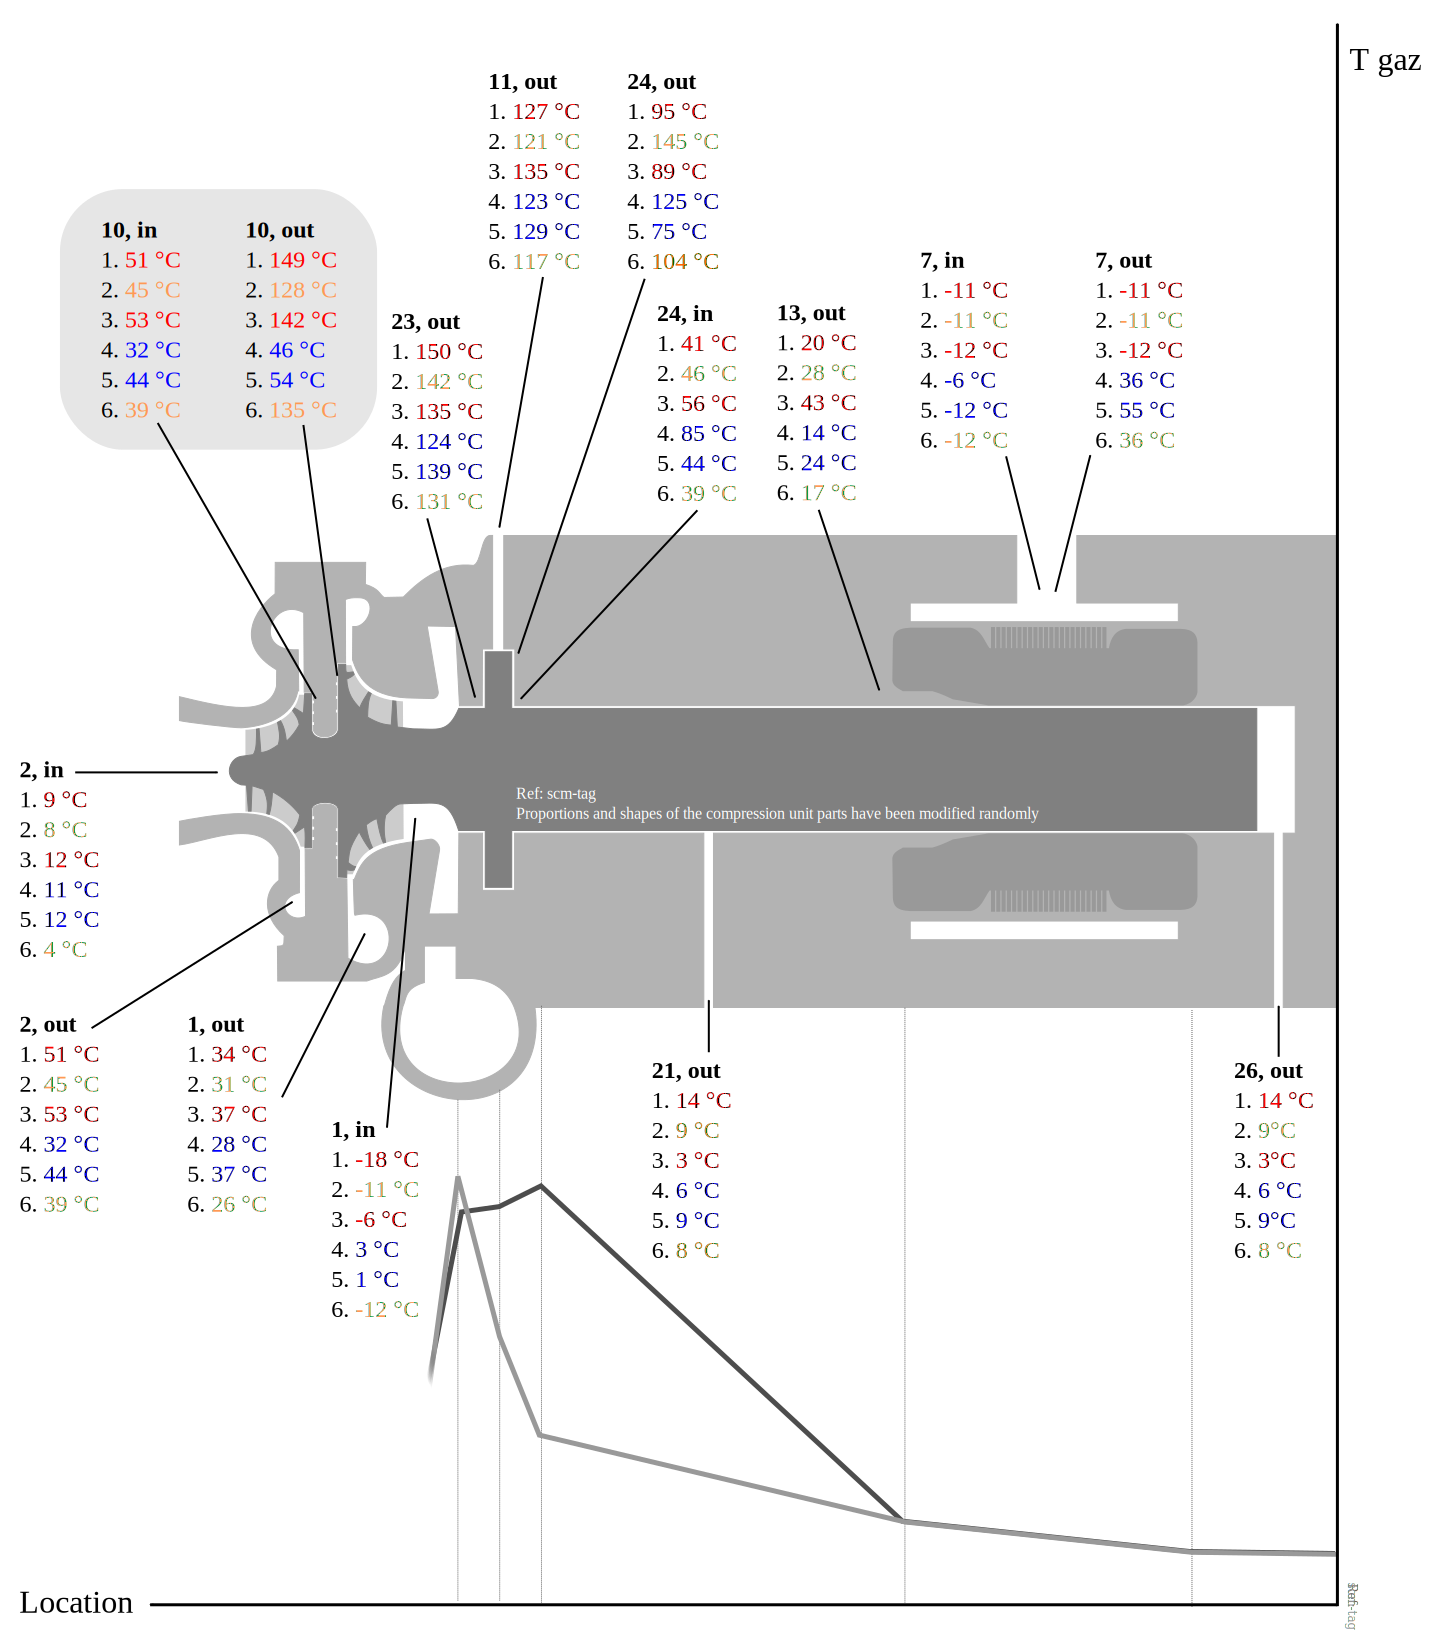
\includegraphics[width=1.0\textwidth]{cp105-awp-expT}
  \caption[Gas temperatures inside the compression unit]{Gas
    temperatures inside the compression unit. The temperature values
    are colored according to the level of gas outlet temperature in
    the labyrinth seal (outlet of component \#10). The lines of
    numbers in red have high labyrinth seal outlet temperatures, while
    the lines of numbers in orange have moderate outlet temperatures,
    and the lines of numbers in blue have low outlet temperatures. The
    temperature profiles at the bottom of the picture illustrate
    qualitatively the 2 types of profiles observed.}
  \label{fig:awp-cp-unit-gas-T}
\end{figure}


\subsubsection{Assumptions}
\label{sec:awp-laby-seal-hot-gas-assumptions}


\paragraph{Location of the hottest point}

The results of the solving of the model for each of the stable \OP{},
summarized on \cref{fig:awp-cp-unit-gas-T}, let assume that the
location of the hottest point of the shaft is in the axial bearing
area. In the \OP{} \#1, \#3, \#5, and \#6, it seems to be between the
first stage impeller and the axial bearing. In the \OP{} \#2, and \#4,
it seems to be just at the location of the axial bearing side where
the gas stream flows reversely. This situation comes probably from the
lack of available data to constrain the model proposed in
\cref{sec:awp-model}. Indeed, minimums of the objective function can
currently be observed with more than one flow temperatures and heat
exchange, close to the axial bearing: the temperature peak can be
before or after the axial bearing without making a significant
difference in term of objective function. This situation occurs
because no mass or energy rates and no temperatures are known in this
area. Consequently, as soon as the global balances with the group of
components [\#11, \#12, \#23, \#24] are respected, it makes no
difference for the objective function and it exists more than one
configuration that satisfy the balances. This uncertainty about the
gas thermal profile could be solved easily by introducing a more
detailed thermal monitoring of the compression unit and its flows, as
it would allow to add more constraints in the model objective
function.

\paragraph{Gradient of temperature along the shaft}

The temperatures observed through the solving of the \AWP{} model let
think that the shaft axial thermal gradient is quite strong close to
the bearings area. It could be that the shaft temperature is a lot
higher when the rotor speed is above 160 krpm as a result from
increased windage and parasitic electro-mechanical losses. Perhaps the
shaft temperature, between the impellers and the axial bearing, is a
function of the rotor speed. The shape of this function could be
exponential toward the rotor speed. This assumption can not be checked
in the frame of this work due to a lack of data. If this assumption
appears to be true, it may be that the axial bearing, traveled across
in the reversed way on one of its side, performs badly. It may be that
the relative location of the axial bearing in its gaps is not
appropriate, with this configuration of flow.


\paragraph{Improvement of the thermal design of the
  compression unit}

Thermal management is an important area of the design of such
compression units, since the gaps between the parts are very small and
consequently, the dilatation phenomena have to be taken in account
very carefully. \citet[p.\,3]{Schiffmann-Favrat-2010b} state that the
thermal design and management of the compression unit is very
important to reach a good performance of the device and the integrated
multi-objective design method they propose takes the thermal
management into account through a lumped parameter approach. The unit
has been designed to sustain such high temperature, but with the idea
in mind that the refrigerant used in the heat pump circuits would be
cleared from every trace of lubricant oil. Reaching such high
temperatures could create troubles due to the lubricant pollution
observed in the heat pump circuits\footnotep{The lubricant oil
  pollution issue is detailed in
  \cpref{sec:awp-issue-oil+corrosion}.}. Indeed, the synthetic
lubricant oil, heated up to those temperatures, might start to
deteriorate. The degradation of the lubricant oil creates
uncondensable gases which decrease the heat pump performance, as
those uncondensable gases are pumped in the cycle by the compression
stage without transferring heat energy efficiently from the evaporator
to the condenser.

\subsubsection{Scenarios to test in future work}
\label{sec:awp-laby-seal-hot-gas-next}

\paragraph{Improved thermal management of the unit}

In 2013, \citet[p.\,1--2]{schiffmann-2013a} highlights the importance
of the thermal management in small scale radial compressors. He shows
that the gas bearings losses increase in proportion when the shaft
power decreases \citep[p.\,1 \& fig.\,1 p.\,2]{schiffmann-2013a} and
proposes design guidelines to decrease significantly the bearing
losses \citep[tab. 4 p.\,6]{schiffmann-2013a}. Consequently, a first
improvement would be to use bearings geometries which generate less
windage losses. It could also be possible to decrease the pressure
drop of the filter on the gas bearings aeration circuit, for example
by expanding its surface or integrate some of them in parallel, in order
to increase the mass flow rate in this aeration circuit. This increase
would result in a better heat dissipation in the unit. The shaft could
also maybe be redesigned in order to offer more surface to the aeration
flow, which would result in a better heat dissipation.

Moreover, having such a dissipation of energy in the axial bearing
area implies a high temperature of the impeller, and especially of the
first stage impeller. Part of the heat energy given to the impellers
is dissipated in the gas being compressed and this consequently
decrease the isentropic efficiency of the compression stages. In the
same spirit, the leak mass flow rate from the compression second stage
outlet to the first stage outlet, and the heat exchange happening
inside the seal, imply that the first compression stage isentropic
efficiency appears quite low ($\eta_{cp1,s,ext}$ in
\cref{tab:awp-cp-unit-isentropic-cdtns}). In fact, the first
compression stage isentropic efficiency is quite high ($\eta_{cp1,s}$
in \cref{tab:awp-cp-unit-isentropic-cdtns}), but is decreased a lot by
the leakage. Those phenomena decrease the efficiency of the
compression unit, and consequently, the efficiency of the whole heat
pump cycle.

\paragraph{Correlation of the thermal profile with the rotor speed}

So far, no direct correlation could be found between the energy rate
flowing from the shaft to the impellers $\dotQ{11}{1}$ and the
labyrinth seal (component \#10) outlet temperature $T_{10,\,out}$. It
would be interesting to to study the behavior of the labyrinth seal
more thoroughly. It may be that the design of the seal is not
appropriate to the conditions in the cycle, which would explain at
least partly the huge leaks observed between the two compression
stages. Those leaks are detailed in
\cref{tab:awp-cp-unit-isentropic-cdtns} with the mass flow rate
$\dotM{10}{25}$.

\subsection{Mixing and separating gas and liquid in the
  economizer}
\label{sec:awp-issue-eco-separation}

\Cref{fig:awp-eco-gas-liq-sep-1-to-5} shows the different versions of
the economizer gas/liquid separation
parts. \Cref{fig:awp-eco-flow-rates} illustrates the separation
issues:

\begin{itemize}
\item The liquid is sucked up with a rotative gas flow bringing some
  of the liquid phase at the second stage compressor inlet.
\item The incoming superheated gas from the first stage compressor is
  not mixed properly with the incoming saturated gas/liquid flow
  coming from the second stage expansion valve. The gas in the
  economizer stays slightly superheated.
\end{itemize}

Those separation and mixing issues have mostly been solved through
different versions of the economizer mixing part. This part has been
improved through the experiments. 5 successive versions have been
used. The final version, the version \#5, can be seen on
\cref{fig:awp-eco-gas-liq-sep-5} and allows a satisfactory gas/liquid
mixing, resulting in a gas stream with less than 2 degrees of
superheating leaving the economizer, and a satisfactory gas/liquid
separation, blocking the swirling liquid phase streaming up along the
walls of the economizer.

\subsection{Decreasing the performance by using a
  4-way valve}
\label{sec:awp-issue-4way}

\begin{figure}[htbp]
  \centering
  \subfloat[A-6.8/W31.3 -- Refrigeration diagram]
  {\label{fig:awp-A-6.8/W31.3-Ph}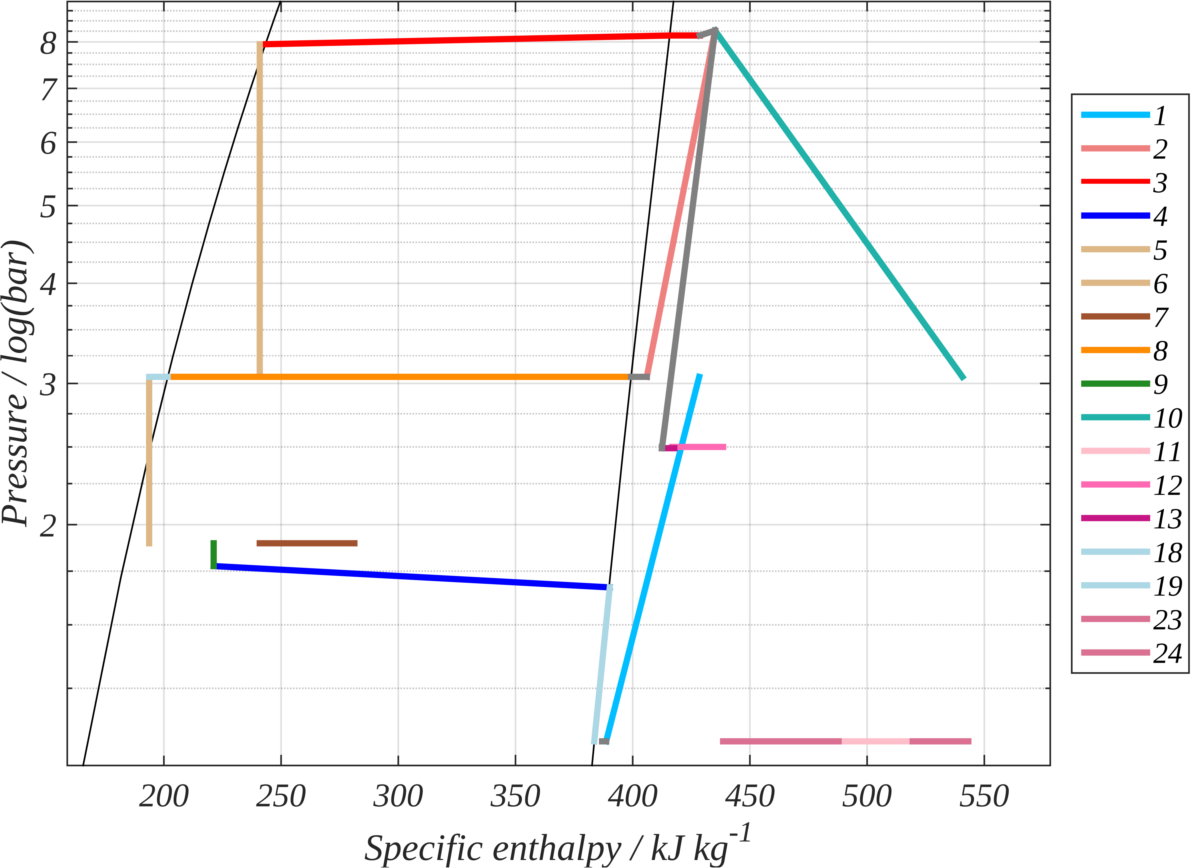
\includegraphics[height=50mm]{awp-Ph-20120511-132418-132718}}
  \hspace{1em}
  \subfloat[A-6.8/W31.3 -- Entropic diagram]
  {\label{fig:awp-A-6.8/W31.3-Ts}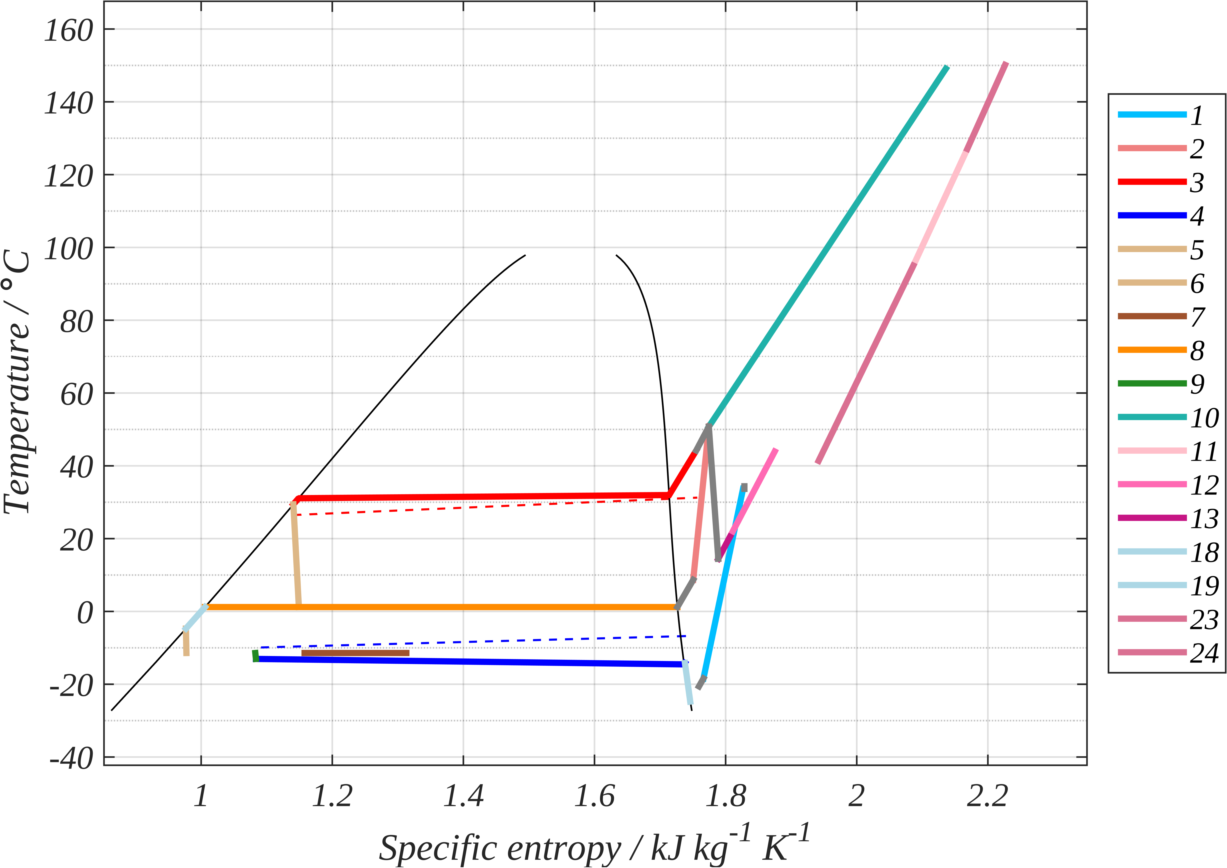
\includegraphics[height=50mm]{awp-Ts-20120511-132418-132718}}
  \\
  \subfloat[A-7.0/W32.3 -- Refrigeration diagram]
  {\label{fig:awp-A-7.0/W32.3-Ph}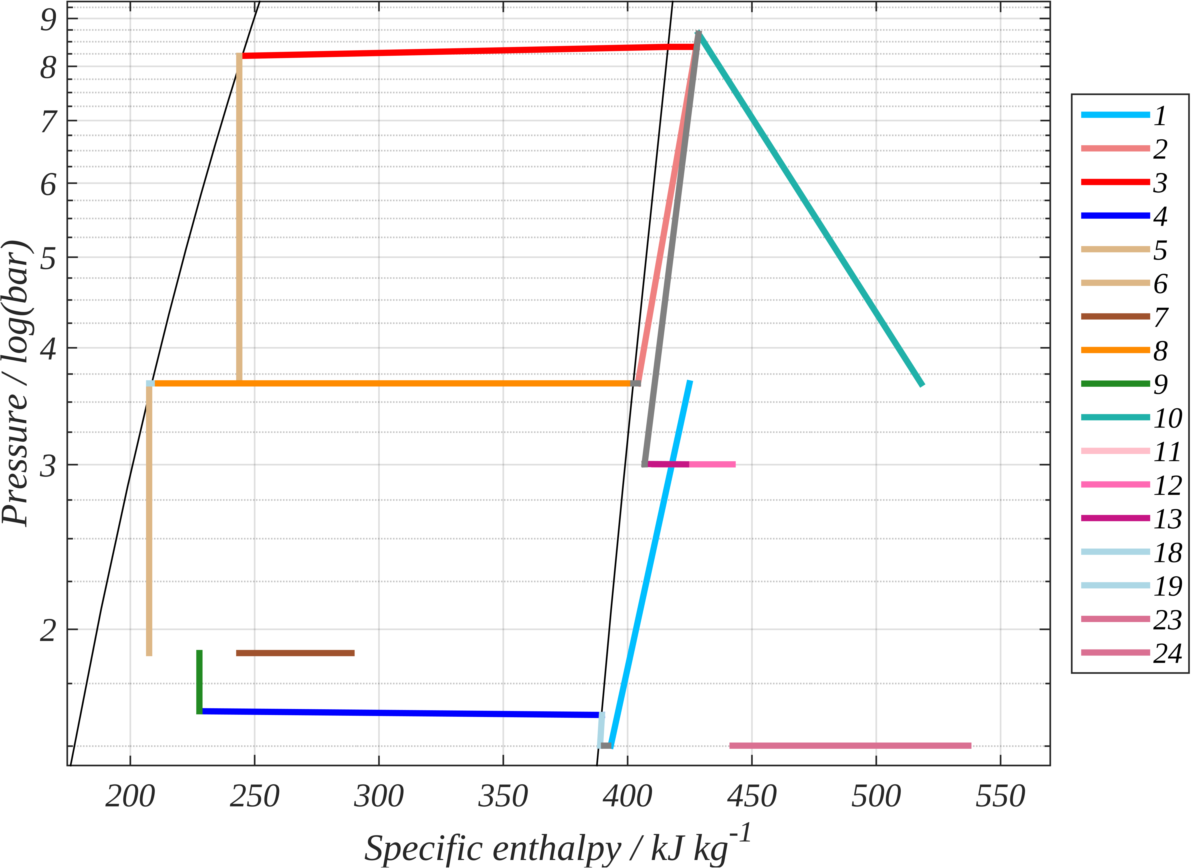
\includegraphics[height=50mm]{awp-Ph-20120531-103842-104143}}
  \hspace{1em}
  \subfloat[A-7.0/W32.3 -- Entropic diagram]
  {\label{fig:awp-A-7.0/W32.3-Ts}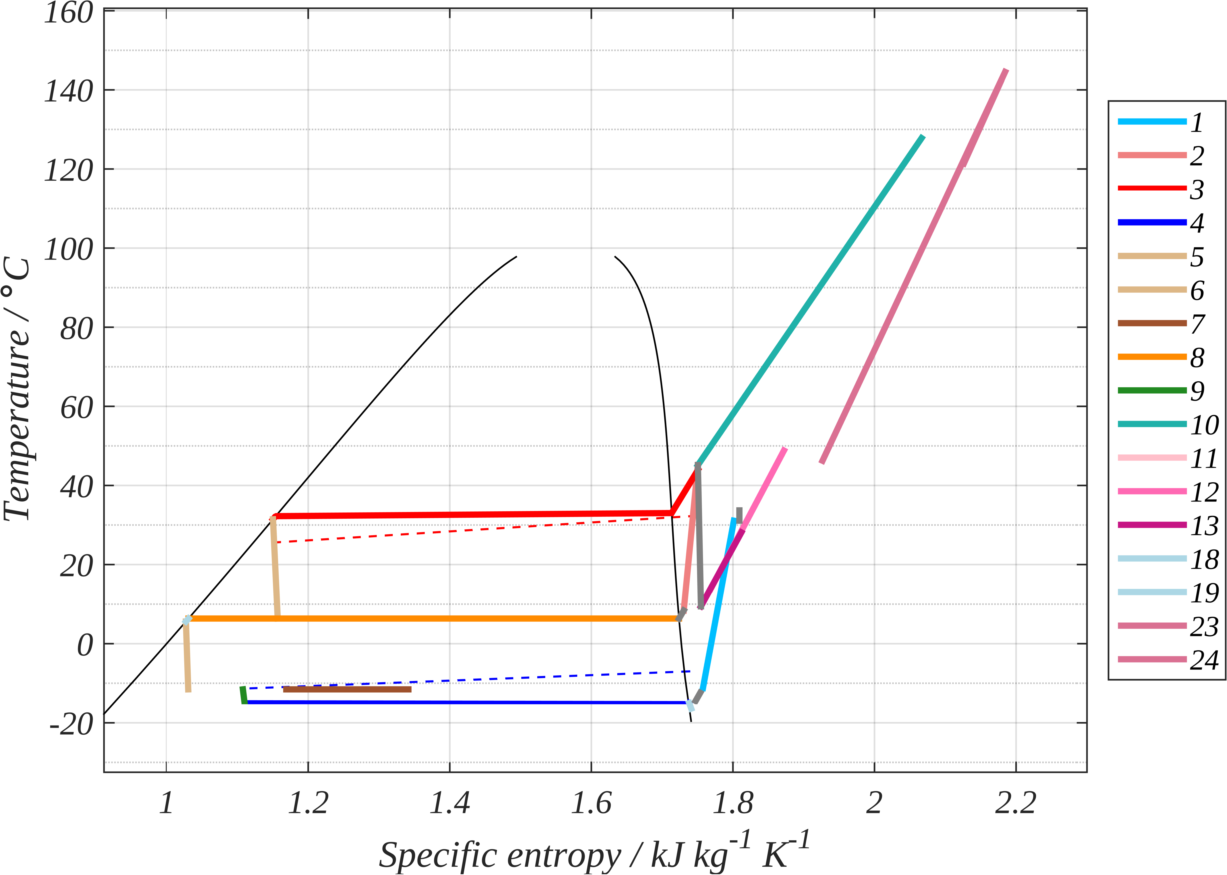
\includegraphics[height=50mm]{awp-Ts-20120531-103842-104143}}
  \caption[A-6.8/W31.3 \& A-7.0/W32.3 -- Thermodynamic diagrams with
  and without 4-way valve]{Thermodynamic diagrams with and without
    4-way valve. OP A-6.8/W31.3 has been recorded with the 4-way in
    the circuit while OP A-7.0/W32.3 has been recorded without the
    4-way valve.}
  \label{fig:awp-w-wo-4way-diagrams}
\end{figure}


The experiments were performed in heating mode. Some of those
experiments were performed with the normal circuit, through the 4-way
valve, and some were performed with a bypass around the 4-way
valve. \Cref{fig:awp-w-wo-4way-diagrams} shows the thermodynamic
diagrams for two similar \OP{}, with and without 4-way
valve. The \OP{} are similar in term of level of temperatures but
there are some significant differences, stressed out in
\cref{tab:awp-4way-differences}\footnotep{More details about those
  \OP{} are available in
  \cref{sec:awp-exp-details-A-6.8/W31.3,sec:awp-exp-details-A-7.0/W32.3}
  page~\pageref{sec:awp-exp-details-A-6.8/W31.3} and page
  \cref{sec:awp-exp-details-A-7.0/W32.3}.}. The pressure drop
difference on the vapor lines can be observed on the enthalpy diagram
and is detailed in \cref{tab:awp-4way-differences}. This example makes
the disadvantage of using a reversing 4-way valve very clear. Indeed,
the valve creates significant pressure drops before and after the
compression stages, decreasing the temperature difference potential of
the device, and generating exergy losses on vapor lines, which are the
worst location to create such losses.

\begin{table}[htbp]
  \begin{center}
    \footnotesize
    \begin{tabular}{lccccccc}
\toprule
OP & speed / krpm & $\dot{Y}_{cd}$ / \si{\kilo\watt} & $\dot{Y}_{ev}$ / \si{\kilo\watt} & $\dot{M}_{ev}$ / \si{\gram\per\second} & COP / - & $\Delta\,P_{4-way}$ / \si{bar}\\
\midrule
A-6.8/W31.3 & \num{170} & $ \num{7.4} \pm \num{0.2} $ & $ \num{4.3} \pm \num{4.3} $ & $ \num{32} \pm \num{2} $ & $ \num{2.19} \pm \num{2.19} $ & $ \num{0.597} \pm \num{0.597} $\\
A-7.0/W32.3 & \num{160} & $ \num{10.5} \pm \num{0.2} $ & $ \num{7.1} \pm \num{0.2} $ & $ \num{37.1} \pm \num{0.9} $ & $ \num{2.69} \pm \num{2.69} $ & $ \num{0.118} \pm \num{0.118} $\\
\bottomrule
\end{tabular}

  \end{center}
  \caption{OP comparison with and without 4-way valve}
  \label{tab:awp-4way-differences}
\end{table}


\subsection{Poor exergy efficiency of the evaporator
  and fluids maldistribution}
\label{sec:awp-issue-reducing-oh}

Maldistribution of the refrigerant and/or of the air in the evaporator
channels has been observed during the experiments. Indeed,
superheating values at the outlet of each evaporator channel vary a
lot, as illustrated
\cref{fig:awp-sh-col-distrib-profile-without-plate}. Difference of
superheat at the outlet of the evaporator circuits can be as high as
8\si{\kelvin}. Consequently, in order to get no liquid phase at the
outlet of the evaporator, high overall superheat values at the inlet
of the first stage compressor had to be imposed. The situation
observed when trying to decrease the superheat value is a good example
of the phenomenon observed by \citet{chen-yezheng-2002a}: indeed, the
superheat may decrease suddenly when it goes down below a certain
value, even if the opening of expansion valve is not changed in the
process. If that amount of superheat was decreased below
4\si{\degreeCelsius}, as illustrated on
\cref{fig:awp-sh-too-low-ev-sh-without-plate}, some liquid was
starting to flow into the first stage separator. Indeed, the liquid
and gas were not mixing together properly after the collector, and a
residual liquid flow was present even with some degrees of overall
superheat in the gas flow.

\begin{figure}[htbp]
  \centering
  \subfloat[Temperatures per circuit, without plate]
  {\label{fig:awp-sh-too-low-ev-T-without-plate}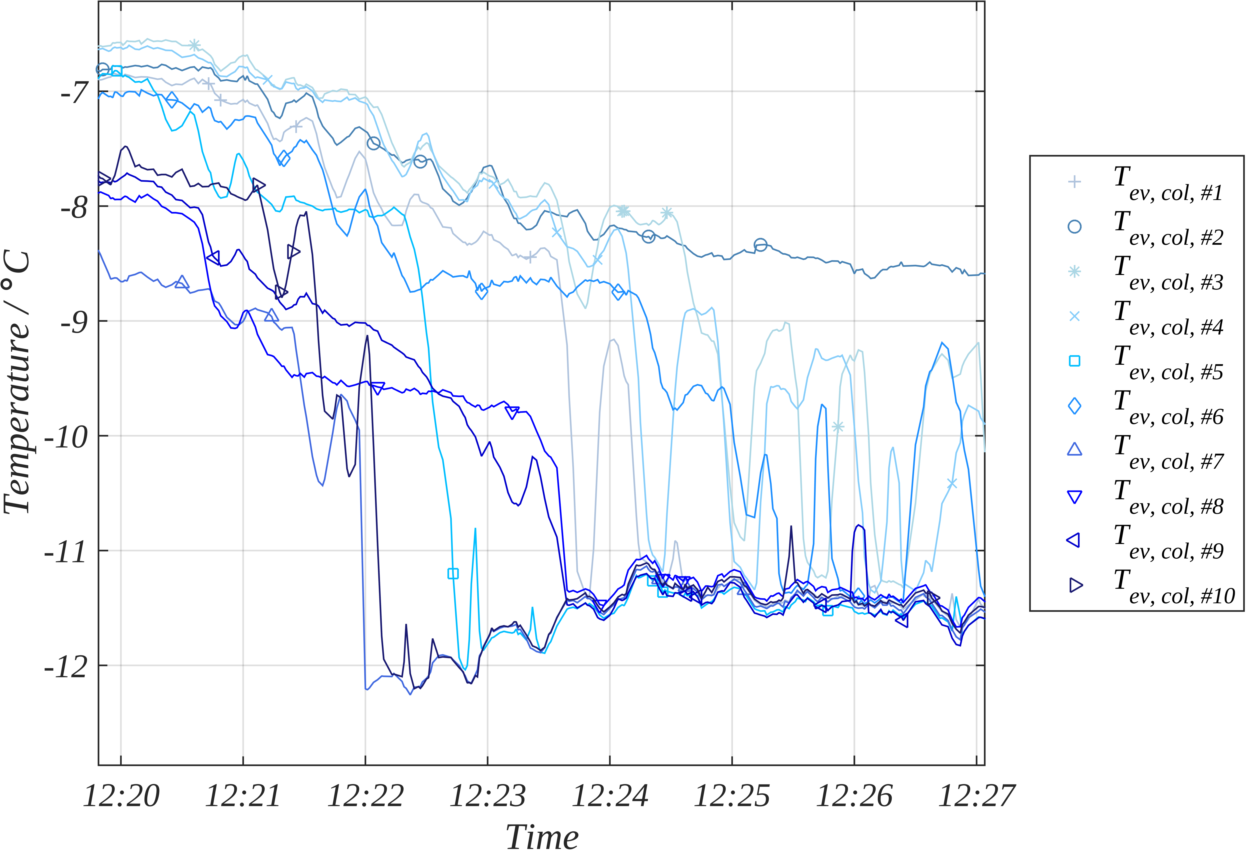
\includegraphics[width=0.45\textwidth]{awp-sh-too-low-ev-T-without-plate}}
  \hspace{1em}
  \subfloat[Temperatures per circuit, with plate]
  {\label{fig:awp-sh-too-low-ev-T-with-plate}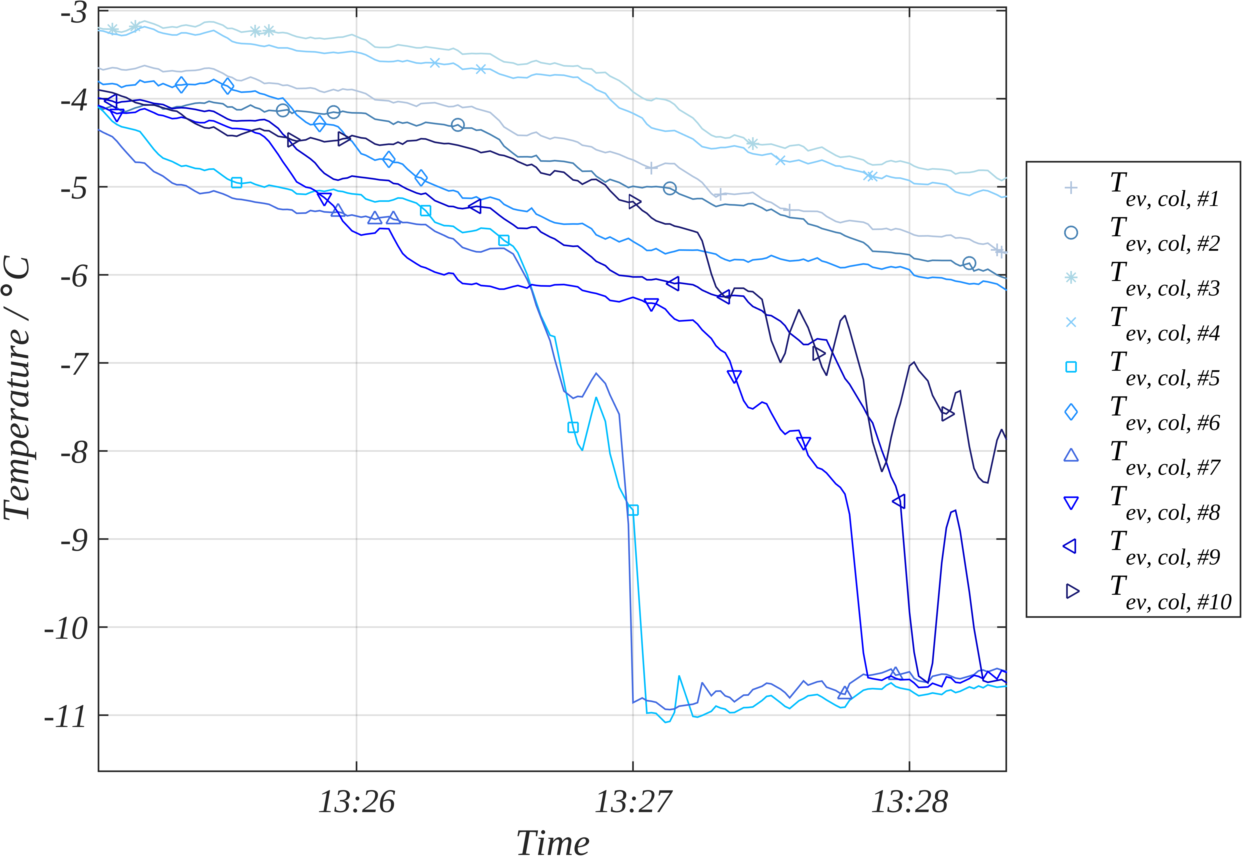
\includegraphics[width=0.45\textwidth]{awp-sh-too-low-ev-T-with-plate}}
  \\
  \subfloat[Superheating per circuit, without plate]
  {\label{fig:awp-sh-too-low-ev-sh-without-plate}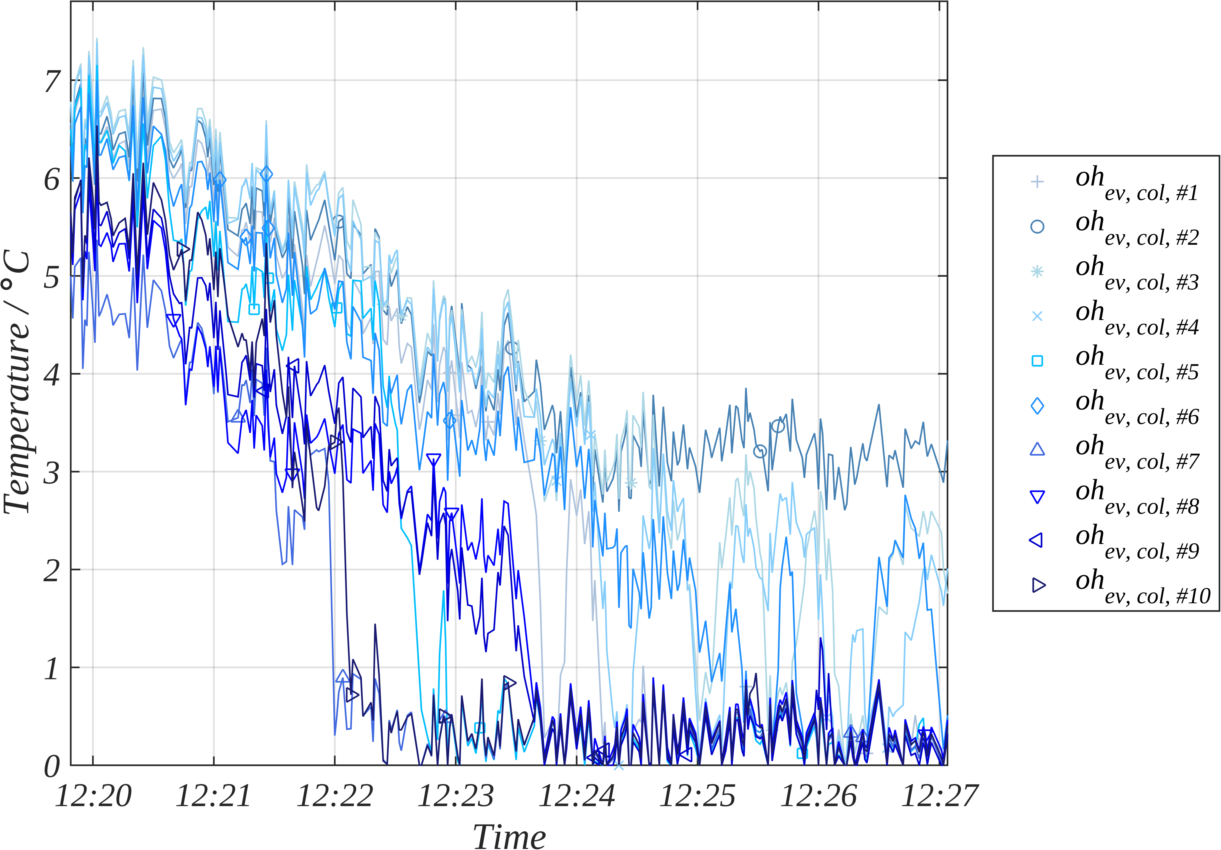
\includegraphics[width=0.45\textwidth]{awp-sh-too-low-ev-sh-without-plate}}
  \hspace{1em}
  \subfloat[Superheating per circuit, with plate]
  {\label{fig:awp-sh-too-low-ev-sh-with-plate}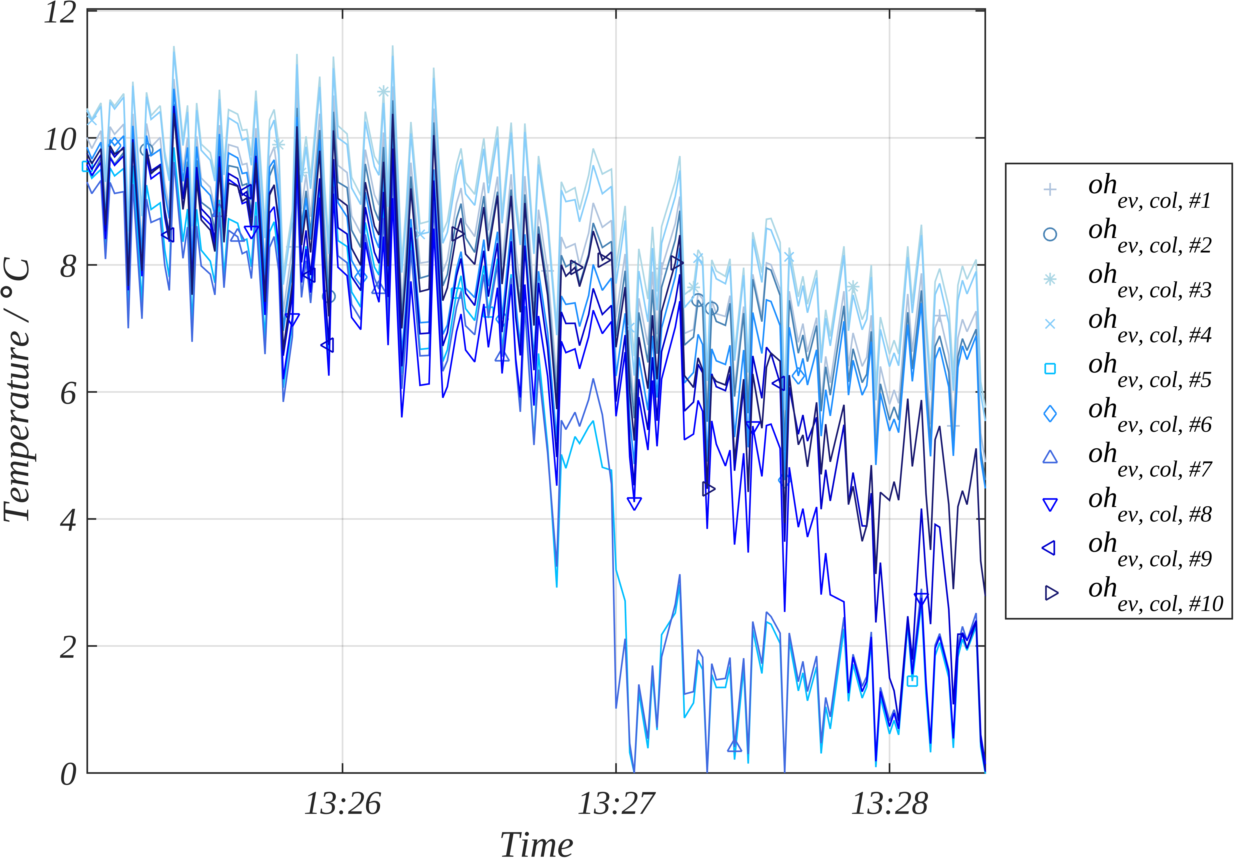
\includegraphics[width=0.45\textwidth]{awp-sh-too-low-ev-sh-with-plate}}\\
  \hspace{0.5em}
  \subfloat[Typical superheating profile, without plate]
  {\label{fig:awp-sh-col-distrib-profile-without-plate}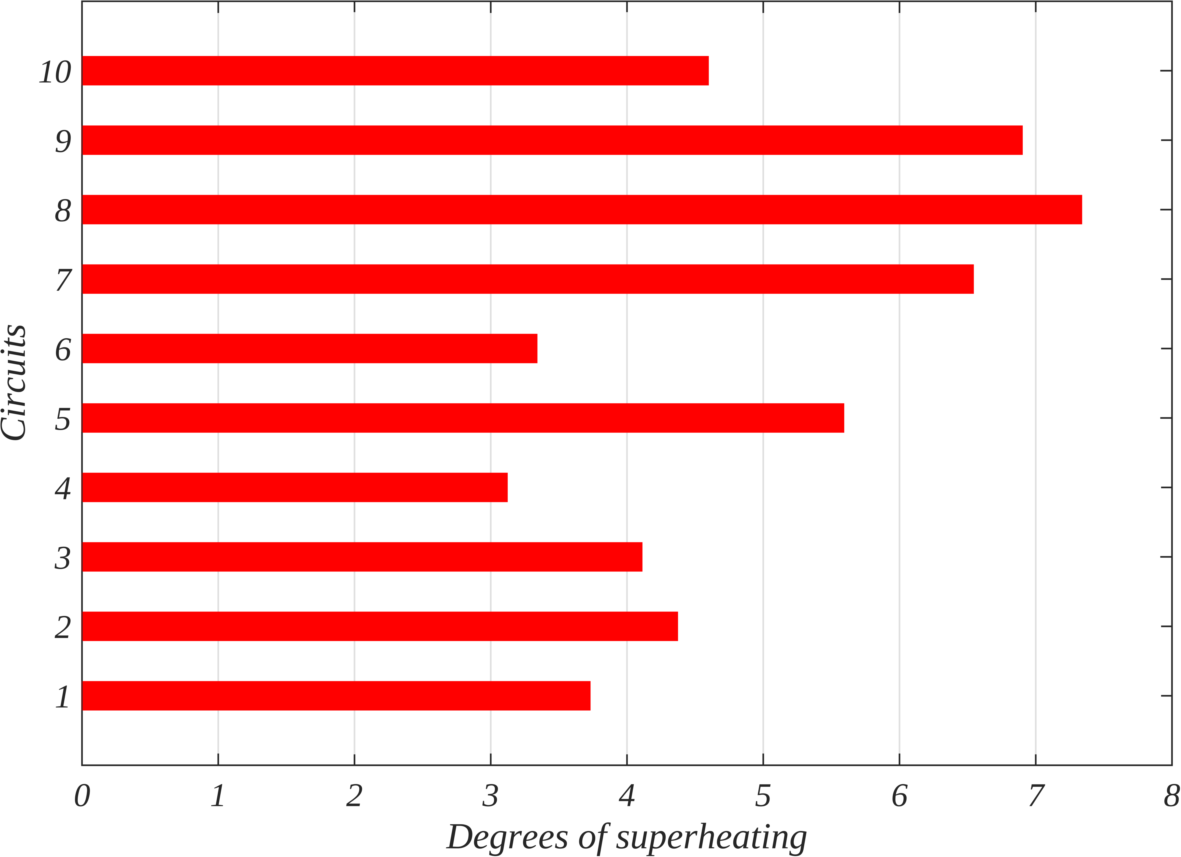
\includegraphics[width=0.35\textwidth]{awp-sh-col-distrib-profile-without-plate}}
  \hspace{5.8em}
  \subfloat[Typical superheating profile, with plate]
  {\label{fig:awp-sh-col-distrib-profile-with-plate}\includegraphics[width=0.35\textwidth]{awp-sh-col-distrib-profile-with-plate}}
  \hspace{5em}
  \caption{Refrigerant and air flow maldistribution in the evaporator}
  \label{fig:awp-maldistribution}
\end{figure}

The maldistribution observed in the refrigerant flow is caused by 2
factors:

\begin{itemize}
\item a non-ideal distribution of the liquid/gas flow coming from the
  lower stage expansion valve, implying that the distribution
  capillaries were not receiving the same mass flow rate and/or the
  same vapor fraction in the flow.
\item a non-ideal distribution of the air flow in the air ducting
  implying uneven speed profiles in the evaporator section. According
  to the location of the fan in the air flow, upper channels are
  clearly exposed to a higher air mass flow rate. Clearly, the design
  of this air ducting emphasizes on compactness, not on effectiveness
  of the heat exchange.
\end{itemize}

None of these two factors could be quantified and studied in
depth. The problem seems to come more from the air ducting than from
the refrigerant distributor, in the experimenter's opinion. In an
attempt to decrease the air flow maldistribution phenomena, a plate
drilled with holes located in front of the evaporator circuits with
the lower superheat values was added 5cm away from the fins, upstream
to the air ducting inlet. The experiments performed after May
$11^{\text{th}}$ 2012 have been performed with this plate fixed
upstream to the air ducting inlet. As illustrated in
\cref{fig:awp-sh-col-distrib-profile-with-plate}, this attempt was a
failure. It even had the tendency to move the average overall
superheat value necessary to ensure the presence of gas only at the
first stage separator to a value increased by about
2\si{\kelvin}. The use of such plate would have been a
temporary solution, in any case, as the plate added a significant
pressure drop in the air flow, and consequently, increasing the
fan energy consumption.

\begin{figure}[htbp]
  \centering
  \includegraphics[width=15cm]{awp-airducting-commented}
  \caption{Air ducting with the fan and the fin-and-tube evaporator}
  \label{fig:awp-air-channel}
\end{figure}

It is possible that the control issue described in
\cref{sec:awp-issue-control} has an influence on the maldistribution
issue, as the refrigerant flow in the evaporator was controlled in an
attempt to get enough superheating at the first compression stage, but
the demonstration performed in \cref{sec:awp-issue-control} shows that
the mass flow rate in the first stage heat pump circuit is a function
of the second stage heat pump circuit mass flow rate and not a value
chosen independently using the first stage expansion valve. Those
elements are detailed further in \cref{sec:awp-issue-control}.

\subsection{Poor exergy efficiency of the subcooler}
\label{sec:awp-low-etaII-sc}

The exergy efficiency of the subcooler $\eta_{sc}$ is defined in
\cref{eq:eta_sc}, p.~\pageref{eq:eta_sc}, and is particularly low. As
detailed in \cref{tab:awp-performances-summary}, $\eta_{sc}$ ranges
from 0.4\% to 3\%. The low performance is the result of a poor
design of the heat exchanger\footnotep{This heat exchanger design is
  detailed in \cpref{sec:awp-subcooler-details}.}, a high temperature
difference between the fluids, and a significant difference of flow
rate between the two streams, as illustrated in
\cref{fig:awp-exp-analysis-model} and \cref{eq:sc-mf},
p.~\pageref{eq:sc-mf}. As it can be seen on
\cref{fig:awp-layout-model-numbers}, the location of the temperature
sensors were also not ideal to quantify accurately this efficiency.

\section{Control issues}
\label{sec:awp-control-issues}

Control issues are related to structural deficiencies and to design
mistakes of the prototype or of the compression unit. As the
prototypes have not been extensively tested, the control strategies
offered in this section and the issues encountered remain poorly
documented. They are mainly a testimony of the experimenter's
experience.

\subsection{Procedure to start the cycle}
\label{sec:awp-proc-start}

As the compression unit is a radial compression machine, it needs to
be equipped with a compressors bypass system. Indeed, in order to
start the installation away from the surge domain\footnotep{See
  \cpref{sec:op-domain} for details about what is the surge phenomenon
  and why avoiding it.}, the characteristics of the circuit needs to
be contained into the operation range of the compressors\footnotep{See
  \cpref{fig:bypass-in-maps} for an illustration of the bypass
  circuits flow characteristics in compression maps.}, represented by
the inner surface of the compressors maps. In heat pump applications,
starting an installation without bypass systems is likely to yield
operation outside of the radial compressor map, at least during the
start-up time. Indeed, in domestic heat pumps applications the sources
temperature levels can not be changed by the heat pump control, as
those temperature levels are imposed by the environment and by the
house. Having defined temperature levels imposes defined pressure
levels at the main heat exchangers and consequently, at the inlet of
the first compression stage and at the outlet of the second
compression stage. For a radial compressor, starting up with no mass
flow rate and an already existing pressure ratio would result in surge
which might damage the compressor. In order to avoid this situation,
the compression unit is started within a bypass circuit which provides
flow resistance characteristics compliant with the compressor
maps. Namely, this implies that the characteristics of the bypass
circuits always fits into the compressors maps, as illustrated
\cref{fig:bypass-in-maps}.

The implemented procedure to start the heat pump prototype is:

\begin{enumerate}
\item Liquid is present at the bottom of the condenser, at the bottom
  of the economizer, and at the inlets of the expansion valves,
  ideally. As the \AWP{} have two separated bypass circuits (one per
  compression stage), it is possible to start with no liquid in the
  economizer, as it was the case in most of the experiments
  performed. In that case, the upper part of the cycle is started
  first while the first compression stage is being bypassed. When
  liquid arrives in the economizer, the lower part of the cycle is
  also started.
\item The compression unit is started at 60 krpm with fully opened
  bypass circuits and fully closed expansion valves.
\item The second stage bypass circuit is closed and the second stage
  expansion valve is opened, but not much. A typical value is 20\% of
  opening for this valve in this situation. As the bypass circuits are
  made of a manual needle valve and a solenoid valve, in the \AWP{},
  the upper part of the cycle switches from the bypass circuit to the
  main circuit instantly, inducing an instantaneous change of pressure
  ratio and mass flow rate in the compression unit. This might induce
  surge at the second stage impeller, if pressure ratio is already too
  high between the economizer (which is approximately at the climate
  chamber temperature and consequently probably at a low pressure
  level as the room temperature might be low) and the condenser (which
  might be at a temperature much higher as the house space heating
  water flows into it). In that case, the compression unit rotor speed
  is increased until the second compression stage leaves the surge
  domain. This happens below 120 krpm in the tested cases.
\item As the upper part of the heat pump cycle stabilizes, saturated
  liquid and gas enters the economizer. The second stage expansion
  valve is set to an opening small enough to increase the pressure
  level at the condenser and get some degrees of subcooling at the
  condenser outlet.
\item The first stage expansion valve is opened with a small opening
  and the first compression stage bypass circuit is closed. Typically,
  the first compression stage enters the surge domain as the pressure
  difference between the economizer and the evaporator is already not
  equal to zero anymore and no refrigerant flows yet through the
  valve, while some gas is being pumped in the evaporator. With no
  flow rate, the compression unit is not able to perform a pump down
  of the evaporator. This needs to be done gradually, and that is also
  why having a controllable bypass circuit has been favored for the
  \BWP{}. Leaving the surge domain is more difficult in this case,
  since this operation implies some increase of the compression unit
  rotation speed, some opening of the first stage expansion valve, and
  depends on the liquid brought at the economizer. If there is no
  liquid in the economizer, it is useless to open the first stage
  expansion valve further. Consequently, starting the lower part of
  the cycle heavily depends of the situation in the upper part of the
  cycle.
\end{enumerate}

With more experience with the setup, this procedure could be
automated. First, the control system could involve level control
devices, and then, with a good knowledge of the device dynamics,
control levels could be removed or kept at their minimal expression
(presence of liquid or not).

\subsection{Procedure to reverse the cycle}
\label{sec:awp-proc-reversing}

The procedure to reverse the cycle is detailed here. It has not been
properly tested as an inversion of the cycle happened only once and
with a low difference between the sources temperature levels.

\begin{enumerate}
\item The heat pump operates at a given \OP{}.
\item Both bypass circuits are opened and expansion valves are closed.
\item The compression unit rotational speed is decreased to 120 krpm
  where the stiffness of the bearings is already good and the rotation
  speed reasonably lowered.
\item The reversing 4-way valve is activated. Liquid might flow from
  the condenser to the first stage separator.
\item The first stage bypass circuit is closed. The first stage
  expansion valve is opened with a small opening. The goal is to get
  an opening big enough to stay away from the surge domain, but small
  enough to create a significant pressure ratio and decreasing this
  way the pressure in the separator. The second stage expansion valve
  is closed and the second stage bypass circuit is opened. The liquid
  in the separator has to be evaporated before increasing the
  compression unit rotational speed too much, in order to prevent
  droplets and liquid suction into the first compression stage. The
  liquid evaporates with the combined action of the energy rate coming
  from the subcooler circuit and the decreasing of the pressure level
  in the evaporator, through the reduction of the first stage
  expansion valve opening.
\item When the liquid in the separator is evaporated, the compression
  unit rotational speed can be increased again.
\end{enumerate}

\subsection{Procedure to stop the cycle}
\label{sec:awp-proc-stop}

\paragraph{During experiments}

During the experiments, the sources temperature levels difference was
gradually reduced in order to be below \num{10}\si{\kelvin}. The
compressor bypass circuits were opened, and the compression unit
rotational speed was reduced to 120 krpm and then, the unit was
stopped.

\paragraph{Normal operation}

Originally, the industrial partner had requested that the filter
included in component \#26 is bypassed by the activation of the
solenoid valve between components \#26 and \#21, in order to set the
pressure levels in the compression unit housing to the intermediate
pressure level before the compression unit deceleration reaches the
dangerous speed zone ranging between 80 krpm and 60
kprm\footnotep{\label{fnote:rot-danger-zone}See
  \cpref{sec:awp-P-balance} for more details about the dangerous
  rotational speed zone.}. This procedure was dangerous, since it
implied the bypass of the filter, which could imply the admission of
dusts of critical sizes inside the radial bearings
cavity (component \#12). Practically,
this procedure has been kept for emergency situations, which did not
occur often, so it is untested. The favored procedure was to lower the
temperature levels difference (reducing consequently the pressure
level differences, which was also reducing the efforts on the axial
gas bearing) and to simply stop the compression unit.

\paragraph{Emergency situations}

In emergency situation, the procedure would be to open the solenoid
valve between components \#26 and \#21, and as the compression unit
starts to slow down, and in any case before the dangerous speed zone
is reached\cref{fnote:rot-danger-zone}, and to open the bypass
circuits while closing the expansion valves. When the compression unit
has stopped, the solenoid valve can be closed again. This procedure
has not been tested during the experimental campaign.


\subsection{Setting an appropriate gas bearings
  aeration circuit flow rate}
\label{sec:awp-issue-bearings-aeration}

Providing the needed gas flow to the gas bearings aeration circuit is
problematic. As described in \cref{sec:cp-intg-aeration}, the 0.5
\si{\micro\meter}-filter is by-far the main pressure drop of the
circuit, which means that the needle valve located before the filter
has a low authority on the circuit flow rate. In fact, the pressure
drop of the filter is too big for the pressure difference observed
between the high pressure zone and the low pressure zone, which
reduces the flow rate possible in the aeration circuit. Practically,
the 1.2 \si{\gram\per\second} measured during the tests could not be
increased significantly. Reducing the flow was also difficult, since
closing the manual needle valve had no consequence with the first
turns, then closing the valve was resulting very fast in a significant
decrease of the flow (the valve was indeed too big and had a low
authority on the flow, but a smaller valve would have decreased the
flow further more). The 0.5 \si{\micro\meter}-filter is necessary to
protect the set of bearings from small dusts that could block grooves
in the set of bearings. The dust-size range to filter here is 0.5 to 5
\si{\micro\meter}, which is the range of dangerous dust size for the
bearings. In order to decrease the filter pressure drop, increasing
the surface of the filter or mounting more filters in parallel would
have been valid solutions.


\subsection{Setting an appropriate motor cooling circuit
  flow rate}
\label{sec:awp-issue-motor-cooling}


\begin{figure}[htbp]
  \centering
  \subfloat[A-3.1/W29.5 -- Refrigeration diagram]
  {\label{fig:awp-A-3.1/W29.5-Ph}\includegraphics[height=50mm]{awp-Ph-20120525-130157-130457}}
  \hspace{1em}
  \subfloat[A-3.1/W29.5 -- Entropic diagram]
  {\label{fig:awp-A-3.1/W29.5-Ts}\includegraphics[height=50mm]{awp-Ts-20120525-130157-130457}}
  \\
  \subfloat[A-6.6/W22.1 -- Refrigeration diagram]
  {\label{fig:awp-A-6.6/W22.1-Ph}\includegraphics[height=50mm]{awp-Ph-20120511-123824-124126}}
  \hspace{1em}
  \subfloat[A-6.6/W22.1 -- Entropic diagram]
  {\label{fig:awp-A-6.6/W22.1-Ts}\includegraphics[height=50mm]{awp-Ts-20120511-123824-124126}}
  \caption[A-3.1/W29.5 \& A-6.6/W22.1 -- Thermodynamic
  diagrams]{A-3.1/W29.5 \& A-6.6/W22.1 -- Thermodynamic diagrams. The
    diagrams illustrate notably a too low mass flow rate in the motor
    cooling chamber, as the vapor quality at the outlet of the motor
    cooling circuit (component \#7) is too high. An other example of
    this situation can be observed for the OP A-0.5/W20.7 in
    \cref{fig:bwp-B8.0/W11.0-A-0.5/W20.7-diagrams}.}
  \label{fig:awp-too-high-motor-cooling-flow}
\end{figure}

\begin{figure}[htbp]
  \centering
    \subfloat[A-7.0/W35.6 -- Refrigeration diagram]
  {\label{fig:awp-A-7.0/W35.6-Ph}\includegraphics[height=50mm]{awp-Ph-20120525-150822-151122}}
  \hspace{1em}
  \subfloat[A-7.0/W35.6 -- Entropic diagram]
  {\label{fig:awp-A-7.0/W35.6-Ts}\includegraphics[height=50mm]{awp-Ts-20120525-150822-151122}}
  \caption[A-7.0/W35.6 -- Thermodynamic diagrams]{A-7.0/W35.6 --
    Thermodynamic diagrams. The diagrams illustrate notably a too high
    mass flow rate in the motor cooling chamber, as the vapor quality
    at the outlet of the motor cooling circuit (component \#7) is
    low. Others examples of this situation can be observed for the OP
    A-6.8/W31.3 and A-7.0/W32.3 in \cref{fig:awp-w-wo-4way-diagrams}.}
  \label{fig:awp-too-low-motor-cooling-flow}
\end{figure}

As it can be observed in the entropy diagrams in
\cref{chap:exp-details}, often, during the experiments, the flow in
the motor cooling chamber was not appropriate. Ideally, the flow of
refrigerant sent to the motor cooling circuit would be fully
evaporated. For \OP{} A-6.8/W31.3, A-7.0/W32.3 and A-7.0/W35.6, the
flow was too high, as the vapor quality at the outlet of the motor
cooling chamber was low. This phenomenon can be observed on the
diagrams in
\cref{fig:awp-too-high-motor-cooling-flow,fig:bwp-B8.0/W11.0-A-0.5/W20.7-diagrams}. In
the contrary, in \OP{} A-0.5/W20.7, A-3.1/W29.5, and A-6.6/W22.1, the
flow was too low and the refrigerant was leaving the motor cooling
chamber with too much superheat. This phenomenon can be observed in
the diagrams in
\cref{fig:awp-too-low-motor-cooling-flow,fig:awp-w-wo-4way-diagrams}. At
this flow regulation problem is added the oil separation problem,
which is detailed in \cref{sec:awp-issue-oil+corrosion}. Indeed, in
the \AWP{}, the motor cooling chamber acts as a lubricant oil
separation device. The compression unit \textit{cp101}, after being
removed from one of the industrial partner installations which used
the same motor cooling system as for the one in the \AWP{}, was
partially filled with synthetic lubrication
oil. \Cref{fig:awp-motor-with-oil} illustrates how the motor cooling
chamber was probably performing with an effective cooling of the upper
part of the motor and a defective cooling of the lower part, mainly
surrounded by refrigerant liquid saturated of lubricant oil. Of
course, the presence of this oil significantly decreases the
performance of the motor cooling system \citep{}, as the gap between
the two walls of the motor cooling chamber is small, and because there
is no circulation of the refrigerant around the motor. A defective
motor cooling system can result in unexpected deformations of the
motor parts, and especially of the shaft and can also result in an
overheat of those parts, damaging them heavily. The mounting of the
magnets on the shaft is also sensitive to overheat. Consequently, a
flow boiling motor cooling system might be a better option for the
motor cooling circuit until clean and lubricant-free refrigerant can
be obtained and guaranteed by the industry supply chain.

\begin{figure}[htbp]
  \centering
  \includegraphics[width=10cm]{motor-cooling-with-oil-schematics}
  \caption[Schematic of the motor cooling chamber filled up with
  lubricant oil]{Schematics of the motor cooling chamber filled up
    with lubricant oil. The cooling down of the motor, symbolized
    qualitatively with the red to blue colors, is not isosymetric
    which could cause dilatation differences and a motor failure.}
  \label{fig:awp-motor-with-oil}
\end{figure}

\subsection{Controlling the heat pump to reach stable OP}
\label{sec:awp-issue-control}

\begin{itemize}
\item Absolute pressure in the economizer (component
  \#8)\index{economizer} was barely affected during the experiments by
  the settings of the prototype, including compressor speed and valves
  settings.
  \item The subcooling value was stabilizing itself around an almost
  fixed value and was independent of the setting of the second stage
  expansion valve.
\end{itemize}

\begin{figure}[htbp]
  \centering
  \includegraphics[width=11cm]{control-ppe-with-2cp}
  \caption[The flow rates of the compression stages are bound
  together]{The mass flow rates of the two compression stages are
    bound together through the pressure levels and current
    compression unit rotational speed. }
  \label{fig:awp-control-ppe-2cp}
\end{figure}

Those two phenomena are explained by the nature of the control system
needed for such a heat pump. If the economizer is perfectly insulated,
the intermediate pressure level is defined by the balance of the
economizer inlet and outlet mass flow rates and enthalpies. Being
external conditions, hot source inlet and outlet temperatures are
imposed. The second compression stage provides the heating service to
the house, so its mass flow rate and pressure level is set by the
external conditions. The intermediate pressure level and the choice of
the compressor rotation speed set the first stage compressor mass flow
rate, as shown in \cref{fig:awp-control-ppe-2cp}. However, the main
function of the first stage expansion valve is to maintain an
overheating value at the first stage compressor inlet. So, the valve,
trying to reach the desired level of overheating, will influence the
first stage mass flow rate and the intermediate pressure level
together.  This will imply the setting of the second stage expansion
valve in order to maintain the second stage mass flow rate, needed to
perform the heating service (change of the intermediate pressure level
implies a change of the mass flow rate if there is no change of the
rotational speed). Consequently, the intermediate pressure level can
not be controlled independently and is a consequence of the choice of
the compression unit rotation speed and the setting of the valves. The
control system needs to control the valves and the rotation speed all
together. Designing such a control algorithm is foreseen as the only
way to control the heat pump in order to reach a stable \OP{} for
every external conditions. This explanation tends to prove that there
is one and only one setting of the valves and rotation speed that
allows to reach a given intermediate pressure level and overheating
value for given external conditions. Of course, this reasoning implies
that the two compressor maps provide a common working point where the
energy and mass balances on the economizer can be satisfied. During
the experiments, the sources temperatures and mass flow rate have been
modified to stabilize the \OP{}, as the heat pump was controlled
manually. Moreover, mass flow rates in the auxiliary circuits, which
have been neglected in this argumentation, have to be taken in account
in the control law and the first assumption of an economizer perfectly
insulated is obviously wrong, which implies that the heat energy
exchanges of the economizer with its environment have an influence on
the control of the heat pump. Finally, it could be also necessary to
modify one of the compression stages with a variable geometry set
up. This modification would allow to adapt the matching of the maps of
the compressors, and to give an additional degree of freedom to the
heat pump controller in order to modulate the heating power.

In order to control the heat pump to reach stable \OP{}, the control
law needs to control simultaneously the rotation speed of the
compression unit, and the settings of the motor cooling valve, the gas
bearing aeration valve, and the two expansion valves. It is mandatory
that the control law controls all those settings together because the
intermediate pressure level is a function of the inlet and outlet mass
flow rates in the economizer and their enthalpies, but the dynamic of
this is very slow. Indeed, what really control the economizer pressure
level is the temperature of the liquid it contains. Consequently, the
intermediate pressure level can not really be set at a chosen value
directly. A control strategy is proposed in
\cref{sec:awp-issue-control-indus}.

\subsection{Control of an industrialized version of the AWP}
\label{sec:awp-issue-control-indus}

In an industrialized product, no mass flow rate is measured. Only
absolute pressures and temperatures are measured.

Pressure levels at the inlets and outlets of the compression stages
are measured, which means that the first and the second pressure
ratios are known. As the compression unit rotation speed is known
through the inverter control, the mass flow rates in the impellers are
known through the use of the compressor maps. But, knowing the mass
flow rates in the impellers does not imply that the mass flow rates in
the different circuits of the heat pump are known. In particular, the
main and auxiliary flows are not quantified, but there is no need to
know then to control the heat pump, as demonstrated in the paragraphs
below.

The second stage flow rate is unknown. This flow rate secures the
product service which is to transfer heat energy to the
house. Functionally, the flow needs to be subcooled when it leaves the
condenser, but the amount of subcooling at the outlet of the condenser
is not controlled properly by the second stage expansion valve, as
explained in \cref{sec:awp-issue-control}. The experimenter recommend
to control the second stage expansion valve with the liquid level in
the economizer. The valve has different control modes. The starting
mode is used if there is no liquid in the economizer or if the
subcooling value is close to zero. In this mode, the valve needs to be
almost fully closed (minimum value, allowing a small flow, and
implying an increase of the second compression stage outlet pressure
through an increase of the pressure level inside the condenser). While
being is this mode, the rotor speed needs to be increased up to a
value high enough to maintain the compression stage outside the surge
domain. This mode can not be used for a long time, as the motor of the
compression unit might not be cooled down efficiently during those
periods for reasons details further in this section. As soon as some
liquid flows in the economizer through the valve, the valve control
law switches to normal mode. In normal mode, the subcooling value is
above zero and the valve is regulated through the level of liquid in
the economizer. If the level decreases, the valve opens. If the level
increases, the valve closes. If the subcooling value falls to zero, in
this case, the valve control switches to starting mode again.

The first stage expansion valve has also different control modes. If
there is liquid in the economizer, the control of the expansion valve
is a classical control which function is to secure a chosen value of
superheat at the outlet of the evaporator (and not at the inlet of the
compression stage). If the level of superheat is too low, the valve
closes, if it is too high, the valve opens. If no liquid is detected
in the economizer, the valve is in starting mode and is fully opened.

With the settings presented above, the intermediate pressure is
defined as the pressure level associated to the temperature of the
liquid refrigerant in the economizer, which is mainly defined by the
second stage expansion valve setting. This implies that the
compression unit can not be used in its more effective range
systematically. If the compression maps and the refrigerant charge in
the installation are correctly optimized, the compression stages
perform in the highest efficiency domains of the compressor maps
during most of the operation time, but this is a consequence of the
optimization of the compressor maps and of the refrigerant charge in
order to get the proper amount of liquid in the economizer when
operating the heat pump at different \OP{}. As explained in
\cref{sec:awp-eco}, the liquid refrigerant which is not in the heat
exchangers at a given time is mainly recovered in the economizer. This
implies that the control law relative to the liquid level management
in the economizer need to be investigated. Indeed, what is the proper
liquid level in the economizer for a given \OP{} is something to be
determined in order to create a good control law. It is important to
note that this proper level is also dependant of the specific
compressor maps of the compression unit powering the heat pump circuit
at the time, which suggests that the controller embeds the maps of the
specific compressor being mounted in the installation and that the
control law are parametrized with parameters of the compressor maps. A
mathematical model of compressor maps is proposed in
\cpref{chap:cp-maps-models}. If such models are used, the parameters
of those maps models could eventually be used to parametrize the
control laws for the economizer liquid level. Moreover, those control
laws might be dependant of the refrigerant charge being filled up in
the circuits and this might be a parameter to include in the control
laws.

The motor cooling valve in starting mode is fully
closed\footnotep{Starting mode is used if there is no liquid in the
  economizer or if the subcooling value is close to zero at the
  condenser outlet.}. In normal mode, it regulates the temperature of
the motor around a chosen value. If the motor temperature is below
the chosen value, the valves closes. If the motor temperature is above
the chosen value, the valve opens. If the motor temperature gets too
high, in any mode, the heat pump shuts down\footnotep{Shutting down
  the heat pump means closing the expansion valve, opening the bypass
  circuits, shutting down the compression unit. Eventually, it means
  bypassing the filter in the gas bearings aeration circuit. This
  later action is discussed in \cpref{sec:awp-proc-stop}.} and issues
an error. The chosen value needs to be determined with performance
tests. It only needs to be high enough to be sure that no condensation
occurs in the compression unit housing.

The gas bearings aeration valve (which is manual for now, but that
would be in the future replaced by an electric valve with a high
authority on the gas bearings aeration circuit\footnotep{This would
  imply to have a lower pressure drop in the 0.5\si{\micro\meter}-filter.}) in
starting mode is fully open. In normal mode, it is controlled with the
temperature of the gas at the outlet of the compression unit gas
bearings aeration circuit. If the temperature is above the chosen
value, the valve opens, if it is below the chosen value, the valve
closes. The chosen value needs to be determined with performance tests. It only needs to be high enough to be sure that no condensation
occurs in the compression unit housing.

The compression unit rotation speed is determined using the two following rules:

\begin{itemize}
\item If the control system is in starting mode, the compressor speed
  increases.
\item If the control system is in normal mode, which means that the
  compression unit speed is high enough to not be in starting mode,
  the compression unit speed is chosen with the compressor maps to get
  the higher efficiency. The higher efficiency can be defined, at
  first, as the best global compression unit isentropic efficiency
  (being the product of the isentropic efficiencies of each
  compression stages), and ultimately, defined as the best accessible
  heat pump effectiveness or, even better, in the author opinion, as
  the best accessible global exergy efficiency for the heat
  pump\footnotep{Those efficiencies and effectiveness are defined in
    \cpref{sec:methodo-indicators}.}. Those best efficiencies can be
  obtained for the controller using a model-based or predictive
  control \citep{Fallahsohi-LinShi-2010a} approach.
\end{itemize}

\FloatBarrier
\bibliographystyle{plainnat}
\bibliography{main}
\label{sec:awp-refs}

\section*{Credits}
\label{sec:awp-credits}
\addcontentsline{toc}{section}{Credits}
\phantomsection

\begin{description}
\item[\figref{fig:awp-housing}] \ccbyropp{2015}.
\item[\figref{fig:awp-air-channel}] \ccbyropp{2015}.
\end{description}


%% Brine-Water twin-stage oil-free domestic heat pump
%% Description, modeling, and results
\chapter{Brine-Water heat pump Prototype (BWP)}
\label{chap:bwp}
\resetallacronyms

\begin{shaded}
  This chapter presents the \BWP{} designed to demonstrate the
  statement detailed in \cref{chap:methodo}. It presents the prototype
  specifications and design, its results, and the encountered issues.
\end{shaded}

\section{Design of the BWP}
\label{sec:bwp-design}

\subsection{Specifications}
\label{sec:bwp-specs}

\begin{description}
\item[Modularity with the components:] The \BWP{} components can be
  changed and many different possibilities can be tested.
\item[Modularity with the thermodynamics cycles and circuits:] The
  \BWP{} can test different single and twin-stage heat pump cycles,
  and tolerates modifications of the motor cooling and gas bearings
  aeration circuits.
\item[Liquid refrigerant location monitoring:] The \BWP{} is expected
  to allow the tracking of the liquid refrigerant location within the
  cycle. The amount of refrigerant in the heat exchangers and in the
  economizer needs to be known.
\end{description}

Those 3 guidelines led to the following design choices:

\begin{description}
\item[Many assemblies, as few brazings as possible:] Ideally, the
  whole setup would have been designed with fittings and assemblies,
  in order to keep as few brazings as possible, but it would have
  exceeded the budget allowed for the manufacturing of the
  prototype. As a compromise, the setup was built with brazed
  components, connected to assembly fittings at their interfaces. The
  system was built around modules which could be relocated or
  connected differently, using straight flexible or conventional
  pipes, and fittings.
\item[Flexible pipes to connect the weighted elements:] In order to
  weight the heat exchangers and the economizer properly, those
  components have been hang up to load cells, and connected to the
  main circuits using straight flexible pipes. This configuration can
  be observed in \cref{fig:bwp-topology}.
\item[Inline components with selection of the active component:]
  Different types of inline components, such as the expansion valves,
  could be mounted together in parallel in the experimental setup and
  could be operated, alone, or together with the other components of
  the line. This possibility allows to test during the same experiment
  different technologies of valves and active components, in order to
  observe the dynamic response of the cycle\footnotep{An example of a
    test section of expansion devices mounted in parallel can be seen
    in \cpref{sec:bwp-exp-devices}.}. As radial compression units have
  continuous dynamic behavior, changing the dynamics of the valves
  response with different technologies\footnotep{Modulating
    refrigerant valves equipped with a magnetic actuator have a
    response time shorter than stepper-motor valves, but are more
    expensive, for instance. The later valves also have a continuous
    setting behavior while pulse width modulation electric expansion
    valves have a discreet setting behavior. Thermostatic expansion
    valves are cheap but can not be set interactively for the needs of
    the cycle control. Those different technologies have different
    dynamic responses which can have an influence on the dynamic
    behavior of the whole prototype, as the compression unit is a
    dynamic compressor.} can be interesting to develop control
  strategies for the prototypes.
\end{description}

\subsection{Description}
\label{sec:bwp-description}

The \BWP{} is designed to be modular and allows to test different heat
pump layouts. Indeed, each component test section is connected to
other components using fastened fittings and flexible pipes. The
components can be moved and spatially rearranged in the housing. Their
order can also be modified. The experimental setup has been designed to
test single and twin-stage heat pump cycles. The setup is equipped
with load cells to measure the weight of the elements which are
subject to variations of their overall refrigerant vapor
quality. Those weighted components are the condenser, the evaporator,
and the economizer. The weight of the elements was intended to be used
to track the location of the liquid charge in the installation and
would have allowed to compare the observed liquid location behavior
with the predicted behavior using a model of the heat pump integrating
nowadays modeling techniques such as components dynamic modeling and
other techniques listed by \citet{Ding-2007a}. The model in
question would have been based on moving boundaries heat exchanger
modeling, such as the one implemented by \citet{Bell-Lemort-2015a},
and on mass and energy balance equations. The inline components, such
as the expansion valves, can be mounted in parallel in order to be
tested sequentially or together during the same experiment. Before the
experiment presented in this chapter, the \BWP{} had been modified in
order to get a new bypass circuit which was likely to solve the issues
encountered with the \AWP{} and detailed in
\cref{sec:awp-P-balance}. As explained in \cref{sec:bwp-cp-unit}, the
compression unit crashed soon after the beginning of the experiment
because of an assembly issue in the compression unit. Before the crash
of the unit, a small B8.0/W11.0 \OP{} was being stabilized, with the
compressors being connected in series, bypassed with the new bypass
system. This experiment is interesting as it confirms that the new
bypass circuit, described in \cref{sec:bwp-bypass-system}, is
functional and could consequently maybe solve the issue described in
\cpref{sec:awp-P-balance}. It also shows a thermal behavior of the
compression unit very different of the one observed in the \AWP{}.

\begin{figure}
  \centering
  \includegraphics[height=10cm]{bwp-topology}
  \caption{BWP topology, after the first set of heavy modifications
    mentioned in \cref{sec:bwp-redesign-1}.}
  \label{fig:bwp-topology}
\end{figure}

\begin{figure}
  \centering
  \includegraphics[height=10cm]{20130924T174303-3832-mod}
  \caption{View of the experimental setup in the laboratory.}
  \label{fig:bwp_main_view}
\end{figure}

\begin{figure}
  \centering
  \includegraphics[width=1.0\textwidth]{bwp-layout-maillefer}
  \caption[Layout of the Brine-Water heat pump test-rig]
  {Layout of the Brine-Water heat pump test-rig.}
  \label{fig:bwp-layout}
\end{figure}

The \BWP{} has been designed vertically for liquid management
reasons. Indeed, when the heat pump is stopped:

\begin{itemize}
\item Liquid refrigerant tends to condensate at the evaporator, which
  is the coolest location in the heat pump cycle. Consequently, if no
  insulation valve stops this phenomenon, the evaporator tends to fill
  up with liquid when the installation is stopped.
\item Pumping down the evaporator using radial compression units is a
  difficult operation, as a pump down of the evaporator requires to
  decrease its pressure level, and consequently to support a pressure
  ratio at the first compression stage, which implies to have a flow
  there, but there can be enough flow, as the expansion valve is not
  loaded with liquid refrigerant. \Cref{sec:pump-down-ev} presents the
  issue relative to the pump down of the evaporator.
\end{itemize}

\section{BWP components}
\label{sec:bwp-main-components}

This section gives details about of the main components in order to
make the understanding of the
\crefrange{sec:bwp-model}{sec:bwp-issues} easier. Further details
about the components and the topology of the circuits are given in
\cpref{chap:bwp-components}.

\subsection{Compression unit}
\label{sec:bwp-cp-unit}

The compression unit mounted in the \BWP{} for the experiment which
has been used to generate the data presented in \cref{sec:bwp-perfs}
was the \textit{cp101} unit, from the \textit{evo4} design
family\footnotep{Details about the previous design families are given
  in \cpref{sec:bwp-history}.}. This compression unit has been mounted
in the \BWP{} following the piping layout detailed in
\cref{fig:cp101-struct-bwp}. The compression unit mounted in the
circuits can be seen in \cref{fig:bwp-cp101-mounted}. This piping
layout is very different from the one used with \textit{cp105} in the
\AWP{}. Indeed, the unit \textit{cp101} has been plugged in the heat
pump circuits with the proper inlets and outlets
connections. Unfortunately, due to an assembly issue, the unit crashed
soon after the start of the experiment. After dismantling and
investigation at the industrial partner facility, it appeared that the
unit would have broken in any case due to the mounting defect and the
experiment itself is not responsible for the crash.

\begin{figure}
  \centering
  \includegraphics[width=\linewidth]{cp101-wheel-details-bwp}
  \caption[Structure of the compressor unit with the BWP gas bearings
  aeration circuit I/O layout]{Structure of the twin-stage compressor
    unit with the BWP gas bearings aeration circuit I/O layout}
  \label{fig:cp101-struct-bwp}
\end{figure}

\begin{figure}
  \centering
  \includegraphics[width=15cm]{20130924T174605-3852-mod}
  \caption{Compression unit \textit{cp101}, mounted in the BWP}
  \label{fig:bwp-cp101-mounted}
\end{figure}

\subsection{Bypass system}
\label{sec:bwp-bypass-system}

The bypass circuit connects the outlet of the second compression stage
to the first stage separator (component \#8\footnotep{Components
  numbering is detailed in \cpref{fig:bwp-layout} and
  \cpref{fig:bwp-maillefer-break-model}}). When the bypass circuit is
used, the solenoid valve in component \#27 is open and no gas from
the vapor line flows into the economizer (component \#9). The
economizer is consequently, in bypass-mode, a simple tank located
after the second-stage expansion valve, ensuring that the first stage
expansion valve is filled up with liquid. In that mode, the economizer
as only one inlet and one outlet\footnotep{In the \AWP{}, the
  economizer has 2 inlets and 2 outlets in every modes.}. In the
\AWP{}, each compression stage has its own bypass-mode and can be
bypassed separately. In the \BWP{}, in bypass-mode, the two
compression stages are in series. The two compression stages have the
same mass flow rate and the intermediate pressure is kept at the
economizer pressure using the second expansion valve
only\footnotep{See issues in \cpref{sec:awp-issue-control}, and
  \cref{sec:bwp-bypass-mode-Pint-issue}, for details about keeping the
  intermediate pressure at a chosen value.}, as the first expansion
valve is dedicated to the setting of the superheat at the outlet of
the evaporator. \Cref{fig:bypass-schematics} shows the complexity of
the configuration of the flows when being in bypass-mode, for the
\AWP{} (\cref{fig:awp-bypass-simple-layout}) and \BWP{}
(\cref{fig:bwp-bypass-simple-layout}). It shows also that the bypass
circuit resistance flow characteristic needs to always be contained in
the compressor maps in order for the bypass to ensure their
function. Those characteristics are illustrated in
\cref{fig:bypass-in-maps}. The layout of the bypass circuit can be
observed in \cref{fig:bwp-layout}. The circuit is the component \#8.

\begin{figure}[htbp]
  \centering
  \begin{minipage}[r]{0.5\linewidth}
    \begin{flushright}
      \subfloat[AWP simplified bypass circuits layout]
      {\label{fig:awp-bypass-simple-layout}\includegraphics[width=\linewidth]{awp-bypass-mf}}
      \\
      \subfloat[BWP simplified bypass circuit layout]
      {\label{fig:bwp-bypass-simple-layout}\includegraphics[width=\linewidth]{bwp-bypass-mf}}
    \end{flushright}
  \end{minipage} \hfill
  \begin{minipage}[l]{0.48\linewidth}
    \begin{flushleft}
      \subfloat[Bypass circuits characteristics in compressor maps]
      {\label{fig:bypass-in-maps}\includegraphics[width=\linewidth]{bypass-in-maps}}
    \end{flushleft}
  \end{minipage}
  \caption[Compressors bypass systems in the AWP and the
  BWP]{Compressors bypass systems in the AWP and the BWP. Those
    schematics are simplified layouts. The complete layouts are
    available in \cref{fig:awp-layout-model-numbers,fig:bwp-layout}.}
  \label{fig:bypass-schematics}
\end{figure}

\subsection{Motor cooling circuit}
\label{sec:bwp-motor-cooling}

The motor cooling circuit in the \BWP{} takes in account the motor
cooling issue encountered with the \AWP{} and detailed in
\cpref{sec:awp-issue-motor-cooling}. The motor cooling strategy in the
\BWP{} is based on a flow-boiling heat exchange while the strategy in
the \AWP{} is a pool-boiling strategy. Pool boiling is easier to
control as a simple liquid level management would be enough to ensure
the proper cooling down of the motor. As lubricant pollution is
encountered in the heat pump circuits\footnotep{This motor cooling
  issue is detailed in \cpref{sec:awp-issue-oil+corrosion}.}, flow
boiling was a better technical solution in polluted
circuits\footnotep{Details about the design and layout of the \BWP{}
  motor cooling circuit are given in
  \cpref{sec:bwp-motor-cooling-details}.}. The compression unit inlets
and outlets could be closed with ball valves, in order to be able to
remove the unit from the circuit without recovering the refrigerant
from the installation. The layout of the motor cooling circuit can be
observed in \cref{fig:bwp-layout}. The circuit is the component \#7.

\subsection{Gas bearings aeration circuit}
\label{sec:bwp-aeration}

The \BWP{} gas bearings circuit\footnotep{Further details about the
  BWP gas bearings aeration circuit can be found in
  \cpref{sec:bwp-aeration-details}.}  is similar to the \AWP{}, but
has the following main differences:

\begin{itemize}
\item The topology of the circuit is more vertical than in the \AWP{},
  and the pipes are longer. As a result, the pressure drop in the
  pipes is higher, and the chances of gas condensation in the pipes
  are also higher. However, the risk of condensation is decreased by
  the fact that the BWP is kept at room temperature, while the AWP was
  in the climate chamber, and was consequently at the environment
  temperature.
\item There are two 0.5\si{\micro\meter}-filters (one per circuit
  branch). Consequently the pressure drop created by the filtration
  process is lower.
\end{itemize}

The layout of the gas bearings aeration circuit can be observed in
\cref{fig:bwp-layout}. The circuit is made of the components \#21,
\#22, \#26, and of the pipe connecting component \#12 to component
\#19. The new layout was expected to solve the issue detailed in
\cpref{sec:awp-P-balance}. Unfortunately, the data collected and the
test performed did not allow to confirm the solving of the issue
with the new system, as the compression unit broke before a proper
stop sequence could be studied. Consequently, further tests with new
compression units and the next version of the experimental setup need
to be performed with the improved bypass circuit in order to document
the new system and its results.

\section{Modeling}
\label{sec:bwp-model}

The model proposed is based on the areas or physical elements of
interest in the \BWP{}. \Cref{fig:bwp-layout} presents the \BWP{}
layout and \cref{fig:bwp-maillefer-break-model} presents the model
itself. The set of equations deduced from analysis of the model in
\cref{fig:bwp-maillefer-break-model} is detailed in
\cref{chap:bwp-eqn}. Following the procedure described in
\cpref{sec:methodo-models}, the model is built with 27 components; 10
of them describe the compression unit itself.

\begin{figure}
  \centering
  \includegraphics[width=0.95\textwidth]{bwp-maillefer-exp-analysis-model-break}
  \includegraphics[width=0.95\textwidth]{bwp-maillefer-exp-analysis-model-break-legend}
  \caption[Modeling of the BWP in bypass mode]
  {Modeling of the BWP in bypass mode. The bypass mode implies that
    the two compression stages are connected in series.}
  \label{fig:bwp-maillefer-break-model}
\end{figure}

\section{BWP results and observations}
\label{sec:bwp-perfs}

The compression unit failed after 25 minutes of experiment, while an
\OP{} B8.0/W11.0 was being stabilized. The \OP{} in question was not
really a conventional \OP{}, as the compression unit was still
bypassed. The experimenter was stabilizing the conditions before
closing the bypass circuit furthermore. Using the model proposed in
\cref{sec:bwp-model}, the amount of the flow being bypassed could be
computed. At the time when the compression unit broke, 61\% of the
flow was being bypassed\footnotep{Ratio of $\dotM{8}{19}$ over
  $\dotM{1}{25}$. The values of those mass flow rate are available in
  \cpref{tab:bwp-B8.0/W11.0-mf}.}, which explains the high level of
superheat observed at the outlet of the first stage separator
(component \#19).

Using the model, the mass flow rates and the energy rates between the
components of the prototype could be computed. They are detailed in
\cref{tab:bwp-B8.0/W11.0-mf,tab:B8.0/W11.0-energy-flows}\footnotep{The
  thermodynamic points, the performance indicators, and the graphs of
  some key values right before the break are available in
  \cpref{sec:bwp-exp-details-B8.0/W11.0}.}. Observing the data
collected from the experiment or determined with the model leads to
the following general observations:

\begin{itemize}
\item Changing the gas bearings aeration circuit inlets/outlets
  configuration used for the \AWP{} to the proper configuration,
  applied in the \BWP{}, seems to change the temperature behavior in
  the compression unit, as it can be observed in
  \cref{fig:bwp-B8.0/W11.0-Ts}, compared with the behavior observed
  with the closest \AWP{} \OP, represented in
  \cref{fig:awp-A-0.5/W20.7-Ts}, where the temperature was increasing
  a lot less in the aeration circuit.
\item The motor cooling flow was too high. This was done on purpose,
  in order for the experimenter to be able not to worry about the
  cooling of the motor during the start-up phase of the
  experiment. The compression unit internal temperature was monitored
  with a PT100 inside the compression unit. The PT100 was located on a
  metal part surrounding the radial bearings cavity. At the time of
  the break, the temperature was of about
  35\si{\degreeCelsius}\footnotep{This temperature was screened on an
    independent device and was not recorded by the data acquisition
    system.}.
\item \Cref{tab:bwp-B8.0/W11.0-mf} shows that there was approximately
  no flow in the labyrinth seal\footnotep{Component \#10.}, and that
  this flow was almost adiabatic, which seems to indicate that the
  shaft was not at a high temperature at the time and that the
  impellers were at a temperature close to the second stage gas outlet
  temperature.
\item The gas in the bypass circuit (component \#8) was not increasing
  its temperature too much despite the relatively long period of
  bypassing involved\footnotep{The bypass circuit has been partially
    open for the whole time of the experiment: 25 minutes. Despite
    this, the gas temperatures were reasonable, as it can be observed
    in \cpref{tab:B8.0/W11.0-PThs}.}.
\end{itemize}

\Cref{tab:key-values-comp-awp-bwp,fig:bwp-B8.0/W11.0-A-0.5/W20.7-diagrams}
allow to compare the situation between the lower \OP{} from the \AWP{}
, the \OP{} A-0.5/W20.7, and the \OP{} from the \BWP{}, to some extents
and on specific topics\footnotep{Original values can be retrieved from
  \cpref{tab:A-0.5/W20.7-PThs}, \cpref{tab:A-0.5/W20.7-energy-flows},
  \cpref{tab:B8.0/W11.0-PThs}, and
  \cref{tab:B8.0/W11.0-energy-flows}.}. The temperature values from
\cref{tab:key-values-comp-awp-bwp} illustrate that the compression
unit thermal behavior is very different in the \BWP{} and in the
\AWP{}. The two \OP{} can not be compared easily as the following
important differences can be observed:

\begin{itemize}
\item The heat energy rate from the motor to the shaft is 5 times
  higher in the \AWP{} \OP{} than in the \BWP{} \OP{}.
\item The \BWP{} \OP{} is recorded at a rotor speed of 110 krpm while
  the \AWP{} \OP{} is recorded at a rotor speed of 130 krpm.
\end{itemize}

Those differences do not formally allow the author to compare the
thermal behavior of the two units. Indeed, the gas inlet temperatures
and rotor speeds are comparable but the heat energy rates from the
motor to the shaft are very different. Consequently the following
comparisons are trends that need to be evaluated with further
experiments, with new compression units in a next version of the
\BWP{}. If the \OP{} would strictly be comparable, the following
interesting points would be interesting to stress:

\begin{itemize}
\item The maximum temperature, occurring in the \AWP{} compression unit
  in the axial bearing, occurs in the \BWP{} compression unit at the
  outlet of the gap between rotor and stator.
\item The maximum gas temperature in the \AWP{} is more than 7 times
  higher than in the \BWP{}. The gas temperature at the outlet of the
  axial bearing sides is only few degrees hotter in the \BWP{}
  compression unit while it is several tenths of degree hotter in the
  \AWP{} compression unit, even despite of the flows in the bearings
  that are in the same order of magnitude in the two experimental
  setups, as the inlet mass flow rate between the two experiments had
  been kept at the same value\footnotep{The mass flow rates in the
    \AWP{} A-0.5/W20.7 \OP{} are available in
    \cpref{tab:awp-A-0.5/W20.7-mf}, and the mass flow rates in the
    \BWP{} B8.0/W11.0 \OP{} are available in
    \cref{tab:bwp-B8.0/W11.0-mf}.}.
\item The temperature of the flow in the labyrinth seal of the \BWP{}
  compression unit is almost constant and is very close to the
  temperature hottest gas flowing in the impellers. This allows to
  think that the impellers temperature was close to
  \num{51}\si{\degreeCelsius} during the \BWP{} \OP{}, as the gas
  temperature reaches \num{51}\si{\degreeCelsius} at the seal outlet
  and as the flow in the labyrinth seal is very small. As stressed in
  \cpref{sec:awp-laby-hot-gas}, the temperature of the impellers in
  the \AWP{} were probably much higher.
\end{itemize}

\begin{table}[htbp]
  \footnotesize
  \centering
\begin{tabular}{lcccccccc}
  \toprule
  \multirow{2}{*}{OP and speed} &
  \multicolumn{2}{c}{Motor} &
  \multicolumn{3}{c}{Gas bearings aeration} &
  \multicolumn{2}{c}{Labyrinth seal}\\
  & $\dotQ{13}{12}$ / \si{\watt} &
  $T_{13,out}$ / \si{\degreeCelsius} & In \#1 / \si{\degreeCelsius} &
  In \#2 / \si{\degreeCelsius} & Out / \si{\degreeCelsius} &
  In / \si{\degreeCelsius} & Out / \si{\degreeCelsius}\\
  \midrule
  B8.0/W11.0, 110 krpm & $\num{11.685} \pm \num{0.003}$ & $\num{17} \pm \num{19}$ & $\pmb{\num{7.90} \pm \num{0.01}}$ & $\pmb{\num{7.98} \pm \num{0.01}}$ & $\pmb{\num{18.95} \pm \num{0.01}}$ & $\num{50.7} \pm \num{0.2}$ & $\num{51} \pm \num{8}$ \\
  A-0.5/W20.7, 130 krpm & $\num{53.060} \pm \num{0.009}$ & $\num{14} \pm \num{23}$ & $\pmb{\num{6.271} \pm \num{0.007}}$ & $\pmb{\num{6.271} \pm \num{0.007}}$ & $\num{123} \pm \num{57}$ & $\num{32} \pm \num{2}$ & $\num{46} \pm \num{21}$ \\
  \bottomrule
\end{tabular}
\caption[Key values for the comparison of the AWP and the BWP gas bearings aeration circuits]{Key values for the comparison of the AWP and the BWP gas bearings aeration circuits, regarding thermal management.}
\label{tab:key-values-comp-awp-bwp}
\end{table}

\begin{figure}[htbp]
  \centering
  \subfloat[B8.0/W11.0 -- Refrigeration diagram]
  {\label{fig:bwp-B8.0/W11.0-Ph}\includegraphics[height=50mm]{bwp-Ph-break}}
  \hspace{1em}
  \subfloat[B8.0/W11.0 -- Entropic diagram]
  {\label{fig:bwp-B8.0/W11.0-Ts}\includegraphics[height=50mm]{bwp-Ts-break}}
  \\
  \subfloat[A-0.5/W20.7 -- Refrigeration diagram]
  {\label{fig:awp-A-0.5/W20.7-Ph}\includegraphics[height=50mm]{awp-Ph-20120531-093353-093653}}
  \hspace{1em}
  \subfloat[A-0.5/W20.7 -- Entropic diagram]
  {\label{fig:awp-A-0.5/W20.7-Ts}\includegraphics[height=50mm]{awp-Ts-20120531-093353-093653}}
  \caption[Thermodynamic diagrams of the BWP OP and of its closer AWP
  OP]{Thermodynamic diagrams of the BWP OP and of its closer AWP
    OP. Those diagrams are presented together in order to give
    comparison opportunities between the two prototypes behavior.}
  \label{fig:bwp-B8.0/W11.0-A-0.5/W20.7-diagrams}
\end{figure}

\begin{table}[htbp]
    \footnotesize
    \begin{center}
      \begin{tabular}{llllll}
\toprule
Name & Value / \si{\gram\per\second} & Name & Value / \si{\gram\per\second} & Name & Value / \si{\gram\per\second} \\
\midrule
$\dot{M}_{1 \rightarrow 25}$ & $ \num{29.2} \pm \num{0.3} $ & $\dot{M}_{2 \rightarrow 8}$ & $ \num{17.8} \pm \num{0.2} $ & $\dot{M}_{2 \rightarrow 10}$ & $ \num{1.88275618e-06} \pm \num{2e-06} $ \\
$\dot{M}_{2 \rightarrow 20}$ & $ \num{10.1} \pm \num{0.2} $ & $\dot{M}_{2 \rightarrow 26}$ & $\pmb{ \num{1.20} \pm \num{1.20} }$ & $\dot{M}_{3 \rightarrow 5}$ & $\pmb{ \num{6.94} \pm \num{6.94} }$ \\
$\dot{M}_{3 \rightarrow 7}$ & $\pmb{ \num{3.20} \pm \num{3.20} }$ & $\dot{M}_{4 \rightarrow 19}$ & $ \num{10.1} \pm \num{0.2} $ & $\dot{M}_{5 \rightarrow 9}$ & $ \num{6.94} \pm \num{6.94} $ \\
$\dot{M}_{6 \rightarrow 4}$ & $ \num{6.94} \pm \num{6.94} $ & $\dot{M}_{7 \rightarrow 4}$ & $ \num{3.2} \pm \num{3.2} $ & $\dot{M}_{8 \rightarrow 19}$ & $ \num{17.8} \pm \num{0.2} $ \\
$\dot{M}_{9 \rightarrow 6}$ & $\pmb{ \num{6.94} \pm \num{6.94} }$ & $\dot{M}_{10 \rightarrow 25}$ & $ \num{1.88275618e-06} \pm \num{2e-06} $ & $\dot{M}_{11 \rightarrow 23}$ & $ \num{0.71} \pm \num{0.71} $ \\
$\dot{M}_{11 \rightarrow 24}$ & $ \num{0.151} \pm \num{0.151} $ & $\dot{M}_{12 \rightarrow 19}$ & $ \num{0.49} \pm \num{0.49} $ & $\dot{M}_{13 \rightarrow 12}$ & $ \num{0.34} \pm \num{0.34} $ \\
$\dot{M}_{19 \rightarrow 1}$ & $ \num{28.5} \pm \num{0.3} $ & $\dot{M}_{20 \rightarrow 3}$ & $ \num{10.14} \pm \num{10.14} $ & $\dot{M}_{21 \rightarrow 13}$ & $ \num{0.34} \pm \num{0.34} $ \\
$\dot{M}_{22 \rightarrow 11}$ & $ \num{0.86} \pm \num{0.86} $ & $\dot{M}_{23 \rightarrow 1}$ & $ \num{0.71} \pm \num{0.71} $ & $\dot{M}_{24 \rightarrow 12}$ & $ \num{0.151} \pm \num{0.151} $ \\
$\dot{M}_{25 \rightarrow 27}$ & $ \num{29.2} \pm \num{0.4} $ & $\dot{M}_{26 \rightarrow 21}$ & $ \num{0.34} \pm \num{0.34} $ & $\dot{M}_{26 \rightarrow 22}$ & $ \num{0.86} \pm \num{0.86} $ \\
$\dot{M}_{27 \rightarrow 2}$ & $ \num{29.2} \pm \num{0.4} $ \\
\bottomrule
\end{tabular}

    \end{center}
    \caption{B8.0/W11.0 -- Mass flow rates between the components}
    \label{tab:bwp-B8.0/W11.0-mf}
\end{table}

\begin{table}[htbp]
    \footnotesize
    \begin{center}
    \begin{tabular}{llll}
\toprule
Name & Value / $W$ & Name & Value / $W$ \\
\midrule
$\dot{E}_{1 \rightarrow 2}$ & $ \num{322} \pm \num{5} $ & $\dot{E}_{11 \rightarrow 1}$ & $ \num{791.8} \pm \num{0.2} $ \\
$\dot{E}_{12 \rightarrow 11}$ & $ \num{824.9} \pm \num{0.2} $ & $\dot{E}_{13 \rightarrow 12}$ & $ \num{844.3} \pm \num{0.2} $ \\
$\dot{E}_{14 \rightarrow 13}$ & $ \num{950.4} \pm \num{0.2} $ & $\dot{E}_{cp1}$ & $ \num{469} \pm \num{5} $ \\
$\dot{E}_{cp2}$ & $ \num{322} \pm \num{5} $ & $\dot{E}_{el \rightarrow 14}$ & $\pmb{ \num{1118.1} \pm \num{0.2} }$ \\
$\dot{Y}_{1 \rightarrow 2}$ & $ \num{2.1718939e-05} \pm \num{1e-07} $ & $\dot{Y}_{2 \rightarrow 10}$ & $ \num{3.71518884e-06} \pm \num{2e-08} $ \\
$\dot{Y}_{3 \rightarrow 15}$ & $ \num{2280} \pm \num{25} $ & $\dot{Y}_{11 \rightarrow 1}$ & $ \num{59.3} \pm \num{0.3} $ \\
$\dot{Y}_{11 \rightarrow 23}$ & $ \num{6.315950126e-07} \pm \num{3e-09} $ & $\dot{Y}_{11 \rightarrow 24}$ & $ \num{0.216} \pm \num{0.001} $ \\
$\dot{Y}_{12 \rightarrow 11}$ & $ \num{29.6} \pm \num{0.3} $ & $\dot{Y}_{13 \rightarrow 7}$ & $ \num{91.31} \pm \num{0.02} $ \\
$\dot{Y}_{13 \rightarrow 12}$ & $ \num{11.685} \pm \num{0.002} $ & $\dot{Y}_{14 \rightarrow at}$ & $ \num{167.72} \pm \num{0.04} $ \\
$\dot{Y}_{16 \rightarrow 4}$ & $ \num{1849} \pm \num{53} $ & $\dot{Y}_{20 \rightarrow at}$ & $ \num{10} \pm \num{10} $ \\
$\dot{Y}_{21 \rightarrow at}$ & $ \num{12} \pm \num{9} $ & $\dot{Y}_{22 \rightarrow at}$ & $ \num{30} \pm \num{22} $ \\
$\dot{Y}_{27 \rightarrow at}$ & $ \num{214} \pm \num{189} $ & $\dot{Q}_{ax}$ & $ \num{33.1} \pm \num{0.3} $ \\
$\dot{Q}_{mo}$ & $ \num{106.12} \pm \num{0.02} $ & $\dot{Q}_{ra}$ & $ \num{19.4} \pm \num{0.3} $ \\
\bottomrule
\end{tabular}

  \end{center}
  \caption{B8.0/W11.0 -- Energy rates between the components}
  \label{tab:B8.0/W11.0-energy-flows}
\end{table}

\section{Additional issues}
\label{sec:bwp-issues}

\subsection{Getting enough power to explore the operation range}
\label{sec:bwp-issue-power}

The compression unit runs at really high speed and consequently needs
an inverter able to provide the needed electric power at the needed
frequency. Finding such an inverter in the current inverter market is
problematic, as high speed drive applications currently applies to
lower electric powers than the one requested for this
work\footnotep{The twin-stage compression unit requires an electric
  power of \num{6} \si{\kilo\watt} to be able to explore its whole
  operation range.}. Consequently, the development of such an inverter
showed up to be necessary and has been performed during an other
thesis work \citep{rod-2012a}. \citet[fig. 6.6, p.\,118]{rod-2012a}
has developed a prototype of inverter which could have been used to
power the compression unit. This prototype needs to be developed
further to become an industrial prototype, ready to used with the
compression units \citep[p.\,134]{rod-2012a}. The experiments have not
been performed with the inverter developed by \citet{rod-2012a}, as it
was still a device in development when the experiments were performed,
and the heat pump prototypes had to cope with the limits of industrial
inverters which were able to explore only partly the compression units
operation domain. Even nowadays, the development and the
industrialization of such an inverter is a critical issue for the
power and control of the heat pumps equipped with such compression
units \citep[p.\,135]{rod-2012a}.

\subsection{Setting the intermediate pressure to a chosen value while being in bypass-mode}
\label{sec:bwp-bypass-mode-Pint-issue}

When being in bypass-mode, the two compression stages have the same
mass flow rate, as they are connected in series. If the flow is only
partially bypassed, the overall pressure ratio is imposed by the
temperature of the sources. As the compression unit rotor speed is a
fixed parameter at a given time, the pressure level between the two
compression stages is a consequence of the compressor maps and can not
be set to a chosen value, as it can be seen in
\cpref{fig:awp-control-ppe-2cp}, considering the same mass flow rate
for the two stages. To be able to close the bypass circuit completely
and to switch to normal-mode, the pressure level in the economizer has
to be kept equal to the pressure level between the compression
stages. If this is not done, the switch can occur nonetheless, but a
pressure shock wave is likely to occur. Because of the check valve at
the first compression stage outlet, the economizer pressure level can
not be below the first stage outlet pressure level, even while being
in bypass-mode. Consequently, the pressure level in the economizer is
necessarily equal (or, eventually, slightly lower\footnotep{Because of
  the pressure drop in the pipes, the pressure level at the inlet of
  the second compression stage can be slightly lower than the pressure
  level at the gas outlet of the economizer.}) or higher than the
pressure level at the second stage inlet. Consequently, the shock wave
will be directed from the second compression stage to the economizer
and will occur when the valve between components \#9 and \#2
opens. This counter flow shock wave can create instabilities in the
flow inside the second stage impeller, damaging blades, or even
produce a compression unit failure. In order to prevent such an event
to occur, the pressure level in the economizer during bypass-mode
needs to be kept at the pressure level of the second compression stage
inlet. This also ensure that no flow comes in the economizer from the
first compression stage.  The pressure level in the economizer while
being in bypass-mode is influenced only by the settings of the two
expansion valves (considering that the economizer is properly
insulated from the environment, and consequently adiabatic). As the
role of the first stage expansion valve is to maintain a superheat
value at the evaporator outlet, even during bypass-mode, the pressure
level is maintained at the second compression stage inlet pressure
level by the second stage expansion valve only. If the pressure level
in the economizer decreases, the valve opens, and if it increases, the
valve closes. If there is no more liquid in the economizer, the second
stage expansion valve closes to a minimal value, in order to let the
pressure level in the condenser increase (this is the second expansion
valve starting-mode explained in \cpref{sec:awp-issue-control-indus}).

\subsection{Pumping down of the evaporator}
\label{sec:pump-down-ev}

In a heat pump circuit, situations might happen where all the liquid
refrigerant charge is located in the evaporator. This is the case, for
example, when you fill in the refrigerant charge in gas phase being
condensed at the coldest location of the circuit (the evaporator). It
can also be the case if the expansion valves are not fully closed when
the installation is shut down and if some time passes between the
shutdown and the next start up (in case of power failure, for
instance). With the bypass system used in the \AWP{}\footnotep{The
  layout of this bypass system can be seen in
  \cpref{fig:awp-bypass-simple-layout} and
  \cpref{fig:awp-layout-model-numbers}.}, it very difficult to pump
down the liquid in the evaporator using the compression unit and the
condenser, as it can be seen in \cref{fig:bwp-pumpdown-ev}. Indeed, as
the bypass circuits are either closed or open (no in-between
position), and as there is no way to create a significant pressure
difference in the heat pump main circuit without closing one of the
bypass circuits (which would most likely results in moving the
compression stages into the surge domain), all the liquid stays in the
evaporator. The only way that could be found during the experimental
campaign was to decrease the temperature at the condenser, allowing to
close the second stage bypass circuit. With the second stage bypass
circuit being closed, the pressure in the condenser increases and the
flows starts to condense. Refrigerant is being transferred from the
evaporator to the condenser. Some liquid finally arrives in the
economizer and the cycle can be started.

\begin{figure}
  \centering
  \includegraphics[width=\textwidth]{bwp-pump-down}
  \caption[Simplified layout in an evaporator pump down situation]
  {When a pump down of the evaporator is needed, most of the liquid
    refrigerant is in the evaporator and as there are almost no flow
    rate through the expansion valves (which are sized to be fed with
    liquid, not with gas), bypass circuits need to be open to avoid
    the surge domain. If the rotor speed is high enough, the pressure
    ratio reached allows to move the check valves and some flow enters
    the main heat pump circuit. Unfortunately, in order to increase
    the pressure ratio in the condenser (which would allow the
    condensation process to occur), the expansion valve needs to
    close, reducing further the flow. The flow is then very small, and
    almost no liquid is transferred from the evaporator to the
    condenser. Meanwhile, there is no flow in the motor cooling
    circuit as there is no liquid in the condenser, and the motor
    temperature increases. It increases even faster as the rotor speed
    is high. If a bypass circuit is closed, the compression stage not
    being bypassed enters the surge domain, as there is not enough
    mass flow circulating in the heat pump circuit and a too big
    pressure ratio. Consequently, if the temperature between the
    sources is not reduced, there is no way to start the heat pump in
    this situation. The new bypass system is expected to solve this
    situation.}
  \label{fig:bwp-pumpdown-ev}
\end{figure}

With the new \BWP{} bypass system, the flow of both compressors is
bypassed together and pumping down the evaporator should not be a
problem. Indeed, the bypass-mode transforms the twin-stage circuit in
a single-stage circuit with the ability to bypass a chosen share of
the flow, and consequently, it should solve the issue described above.

\subsection{Keeping the loop clean}
\label{sec:awp-issue-oil+corrosion}

The prototypes tested use refrigerant with no lubricant. If there is
lubricant in the refrigerant, it causes circuit pollution problems. If
the pollution is not miscible in the refrigerant, it soaks the heat
exchangers surfaces, which is likely to decrease there heat transfer
efficiency \citep{BandarraFilho-Thome-2009a}. If it is miscible, it
decreases the heat power capacity of the heat exchangers. Moreover,
the lubricant is likely to enter the gas bearings and to fill their
grooves, causing their failure and a crash of the compression unit. If
grooves are polluted with oil, the probable consequence is a
displacement of the shaft in the bearing gap, which is likely to cause
a contact between the shaft surface and a fixed part. Touching a fixed
surface at that speed is likely to create torsion forces far beyond
the resistance of the shaft and to break it. Where the shaft touches a
fixed part, the energy released locally is high enough to weld the
surfaces together, damaging the unit massively. Such failures are
critical events and usually imply the full replacement of the
compression unit. Consequently, introducing clean refrigerant in the
heat pump circuits is very important. However, industrial refrigerant
cylinders often contain a small amount of synthetic lubricant
oil. This lubricant oil is likely to pollute the prototype circuits if
filled up with liquid refrigerant\footnotep{Liquid refrigerant can be
  filled in an installation either with a supply bottle put
  up-side-down, or with a recovery cylinder, using the liquid valve,
  which directly get liquid refrigerant from the bottom of the
  cylinder. The recovery cylinders may also contain mineral oil,
  leaked from the vacuum pump, for instance. This oil will be also
  transferred to the heat pump circuits, if they are filled up with
  liquid refrigerant.}. If the prototypes are filled up with gas being
condensed in one of the heat exchangers of the prototypes, some oil
can also pollute the circuits, as the gas velocity is high enough to
drag an oil film, flowing from the cylinder to the circuits of the
prototypes, on the wall of the tubes. In order to prevent oil flowing
from the cylinders to the circuits of the prototypes, gas velocity
needs to be lower than a specific value which can be computed for each
specific design case \citep{kesim-ileri-2000a,Guo-Shen-2011a}. As
those design rules were not applied during the design of the heat pump
prototypes, lubricant oil could be observed flowing slowly from the
inlet of the first stage separator, at the top of the upper flange, to
the outlet, also located at the top of the upper flange, flowing on
the flange surface. The issue has been solved by adding a pipe and a
deflector, inside the separator, in order to make the way from the
inlet to the outlet less straightforward for the oil. The oil
pollution problem has been solved by decreasing dramatically the speed
of the filling up, doing it only with a low velocity, in gas phase. It
is important to note that a polluted installation is very difficult to
clean up, once it has been polluted. The synthetic lubricant oils have
low viscosity and surface tension, so they fill every possible
interstice. Consequently, every O-ring cavity, every welding, every
scratch, every groove or heat exchanger improved surface is polluted
and very difficult to clean up. The problem exists also with the
\AWP{} but extra care and protective behavior being applied from the
start helped to prevent a too high amount of oil pollution in the
circuits.

\begin{figure}
  \centering
  \begin{minipage}[r]{.49\linewidth}
    \begin{flushright}
      \subfloat[Lubricant droplets deposit]{\label{fig:bwp-oil-1}\includegraphics[height=10cm]{20110713T141014-1548d}}
    \end{flushright}
  \end{minipage} \hfill
  \begin{minipage}[l]{.49\linewidth}
    \begin{flushleft}
      \subfloat[Liquid lubricant]{\label{fig:bwp-oil-2}\includegraphics[width=6.45cm]{20110713T134430-1526d}} \\
      \subfloat[Lubricant and dusts]{\label{fig:bwp-oil-3}\includegraphics[width=6.45cm]{DSC00385}}
    \end{flushleft}
  \end{minipage}
  \caption{Lubricant pollution in the BWP}
  \label{fig:bwp-oil-pollution}
\end{figure}

Evaporators act as oil separation devices and tend to collect a good
share of the lubricant oil in the heat pumps circuits. In the \AWP{},
the motor cooling chamber and the evaporator play such a role. In the
\BWP{}, only the evaporator plays such a role, since the refrigerant
flows in the \BWP{} motor cooling chamber from top to bottom,
vertically, towards the evaporator. If the superheat value becomes too
low at the evaporator outlet, refrigerant and oil might flow in the
first stage separator, as illustrated in
\cpref{fig:bwp-oil-pollution}. Synthetic oil is miscible in liquid
R134a and will come with liquid refrigerant more or less
proportionally. Mineral oil, which comes from polluting elements in
the recovery cylinders, and from the vacuum pumps, stays on top of the
refrigerant liquid level. When some liquid comes from the evaporator,
the first amounts are heavily charged with mineral oil, if any is
present in the heat pump circuits. Oil reflux from the vacuum pumps is
something well known in the vacuum industry. Usually, this lubricant
oil is gasified and trapped with a catalyzer containing active
carbon. In the refrigeration industry, nothing is typically done
against those refluxes. Most of the refrigeration professionals even
ignore that such refluxes happen because they are not typically
problematic for the conventional refrigeration technologies, which use
lubrication, and consequently most of those professionals do not learn
the existence of this issue during their certification programs.

\FloatBarrier

\bibliographystyle{plainnat}
\bibliography{main}
\label{sec:bwp-refs}


%% Compressor unit description, modeling, and
%% integration in refrigeration circuits
\chapter{Integration of the compression unit
  in heat pumps layouts}
\label{chap:cp-intg}
\resetallacronyms

\begin{shaded}
  This chapter presents good practices and advanced proposals to
  integrate multistage oil-free variable-speed compression units in
  domestic heat pumps.
\end{shaded}

\section{Topology}
\label{sec:cp-intg-topology}

When using radial compressors, the vertical topology proposed with the
\BWP{} and presented in \cpref{fig:bwp-topology}, is advised. Indeed,
this vertical configuration makes the device more reliable and
increases the chances to collect liquid refrigerant where it is
functionally needed. Most companies building refrigeration circuits
with radial compressors use a vertical topology. The chillers produced
by Smardt\footnotep{Smardt (\url{http://www.smardt.com/}) is a company
  that makes chillers powered by Turbocor compressors. It has been
  created by one of the founders of the Turbocor company, after the
  latter was bought by Danfoss. Turbocor compressors
  (\url{http://www.turbocor.com/}) are radial compressors rotating on
  magnetic bearings. They typically power refrigeration applications
  above 50kW, as the magnetic bearings technology is not easy to scale
  down below this value.} are good examples of this design
rule. Additionally, using the vertical pipes leading to the
compression unit to protect it against the possible presence of
lubricant oil is a good practice. Those pipes can be sized following
the sizing rules presented by \citet{kesim-ileri-2000a} and
\citet{Guo-Shen-2011a}, in order to prevent that the oil is pulled up
with the gas stream.

\section{Electromagnetic perturbations}
\label{sec:cp-intg-electromag}

During the experiments performed with the \AWP{}, the signals of the
sensors where sometimes polluted with high levels of interferences
most probably caused by electro-magnetic perturbations, as the sensor
cables were not shielded. Those electro-magnetic perturbations were
probably generated by the three-phase inverter powering the motor of
the compression unit at high frequencies. Those interferences disturb
the calculation of essential values, like the superheat value. This is
clearly visible in \cpref{fig:awp-sh-too-low-ev-sh-with-plate}, where
the superheat calculation is perturbed (high frequency, high amplitude
signals) by the interferences on the pressure measurements, shown in
\cpref{fig:awp-electromagnetic-perturbation-P}. The temperature
measurements are not disturbed by interferences in that specific case
(as it can be seen in
\cpref{fig:awp-sh-too-low-ev-T-with-plate}). This example highlights
the importance to use shielded cables and grounded-sensors on this
type of device.

\section{Gas bearings aeration circuits}
\label{sec:cp-intg-aeration}

The lowest possible pressure level is favored in the gas bearings
cavity (component \#12) in order to minimize the gas bearings
losses. This implies that the outlet of the gas bearing aeration
circuit is connected to the zone of the heat pump circuit where the
pressure level is the lowest. The best location for this outlet is
consequently in the first stage separator. The inlet of the gas
bearings aeration circuit needs to be located in a zone with a higher
pressure level. Two solutions exist: the inlet can be either at the
intermediate pressure level, in the upper part of the economizer or
between the economizer and the second compression stage inlet, or
either at the higher pressure level, at the outlet of the second
compression stage. In the \BWP{} and the \AWP{}, the safest solution
has been favored: the gas bearings aeration circuit inlet is located
after the second compression stage outlet. This is the safest option,
since the expanded gas has a higher superheat value after its
expansion, if the gas comes from the second compression stage outlet,
and not from the economizer. With the pressure drop observed in the
\AWP{} aeration circuit, using the intermediate pressure level would
have resulted in a lower mass flow rate, which would have been too low
in the tested conditions. However, increasing the surface of the
0.5-\si{\micro\meter}-filter would certainly allow to take the
aeration flow from the economizer. Taking this flow at the economizer
would be better than taking it at the outlet of the second compression
stage, even if it is less safe. Indeed, the aeration flow, if removed
from the second compression stage flow rate, directly impact the heat
pump efficiency, as the flow rate leaving the second compression stage
is used to provide the heating service. The level of superheat would
decrease a little, but this could be compensated with integration
strategies like the one exposed in
\cref{sec:next-topology}. Technically, it seems better to use the
intermediate pressure level to provide the aeration circuit with gas,
but economically, this needs to be studied further, as the filter
surface and volume would increase, in order to compensate for the
decrease of the pressure potential, in order to offer an equivalent
flow rate. This will most probably have an influence on the price of
the filter and consequently, on the price of the heat pump device.

\section{Towards new layouts with improved
  bypass circuits}
\label{sec:cp-intg-new-bypass}

The bypass circuits used in the \AWP{} were far from being
satisfactory, as detailed in \cpref{sec:awp-P-balance}. The bypass
circuit in the \BWP{} apparently performs better but was penalized by
the drawbacks highlighted in
\cpref{sec:bwp-bypass-mode-Pint-issue}. In order to solve this issue,
a new bypass principle is proposed, based on the bypass system of the
\BWP{}. This bypass system is presented in
\cref{fig:bwp-layout-maillefer-next-step,fig:awp-layout-next-step},
adapted to each tested prototype. This new concept mixes the
advantages observed with the economizer of the \AWP{}, which was in
two parts, and the compression stages in series of the \BWP{}. Indeed,
if the two parts of the economizer are connected with a check valve
that opens if liquid weights on it (the spring of the check valve must
be designed for this application, consequently), instead of a straight
pipe, the component \#27 of the \BWP{} becomes unnecessary. When
entering in bypass-mode, the solenoid valve above the pre-mixing
device\footnotep{On the left of the economizer in
  \cref{fig:bwp-layout-maillefer-next-step,fig:awp-layout-next-step},
  p.\,\pageref{fig:bwp-layout-maillefer-next-step}.}  shuts down the
arrival of liquid in the economizer (during this bypass-mode, the
second stage expansion valve must remain at least slightly opened, in
order to prevent a possible pressurization of the pipe between the
expansion valve and the solenoid valve). The liquid in the economizer
leaves into the lower part of the economizer (if there is any in the
upper part). The two compressors are now in series. In this new
bypass-mode, either the heat pump cycle is used, either the bypass
circuit is used (in the contrary of the bypass circuit used in the
\BWP{}, which could be used in parallel of the heat pump circuit). If
the pressure level in the lower part of the economizer changes and
becomes higher than the pressure level in the upper part\footnotep{For
  instance, because some liquid evaporates, if there is any. The
  liquid could be used to cool down the power electronics, for
  instance, which would result in an evaporation of some of the
  fluid.}, the check valve opens and the pressure level are equal
again, which allows the check valve to close again. The pressure level
in the upper part of the economizer is consequently higher or equal to
the pressure level in the lower part. This bypass-mode can be used to
start and stop the cycle, in case of emergency, but also to evaporate
some liquid at the bottom of the first stage separator, as hot gas
returns to the first separator with a high superheat value. As
illustrated in
\cref{fig:bwp-layout-maillefer-next-step,fig:awp-layout-next-step},
the first separator can be equipped with a droplets
deflector\footnotep{A part designed to avoid the suction of droplets
  in the first compression stage.}, and the bypass circuit can deliver
the vapor directly at the bottom of the economizer. Blowing vapor
directly in the saturated liquid can result in the generation of
mist. The author's advice is to use metallic mesh or foam to trap the
droplets at the top of the deflector. This advice applies also to the
concept presented in \cref{sec:next-topology}. Bypass circuits need to
open if there is a power failure. Consequently, that part of the
circuit needs to be equipped with normally opened valves.

\begin{figure}[htbp]
  \centering
  \includegraphics[width=\textwidth]{bwp-layout-maillefer-next-step}
  \caption[Proposal for a new BWP layout]
  {A new BWP layout}
  \label{fig:bwp-layout-maillefer-next-step}
\end{figure}

\begin{figure}[htbp]
  \centering
  \includegraphics[width=\textwidth]{awp-layout-next-step}
  \caption[Proposal for a new AWP layout]
  {A new AWP layout}
  \label{fig:awp-layout-next-step}
\end{figure}

\section{Towards more integration, performance,
  and compactness}
\label{sec:next-topology}

The compression unit may allow a more advanced integration with the
heat pump cycle. This integration would lead to the creation of a
compression module containing many components of the heat pump
cycle. Indeed, the compression module can include easily the current
compression unit, the whole economizer, and the separator. In this
configuration, the only missing components to make a complete heat
pump cycle would be the condenser, the evaporator, the dryer-filter,
the two expansion valves, and the valves for the bypass and the gas
bearings aeration circuit. The module could even include the inverter,
cooled down by the liquid in the economizer. The inverter would be
located directly below the economizer, in that case, and would benefit
from passive convective cooling. As the inline components take almost
no volume, The volume of the installation is made from the volume of
the heat exchangers and of the compression unit module. As detailed in
\cpref{sec:sota-oilfree-hx}, the volume of the heat exchangers can be
decreased by taking advantage of the oil-free heat exchange
technologies. The compression module presented in
\cref{fig:next-prototype} is about 50cm-wide and 30cm-high. This
integration makes also the maintenance easier, as the technician can
unplug the module, and replace it easily. Functionally, such
integration brings many advantages:

\begin{figure}[h!tbp]
  \centering
  \includegraphics[width=\textwidth]{next-prototype}
  \caption{Proposal of an integrated topology for a future heat pump
    prototype}
  \label{fig:next-prototype}
\end{figure}

\begin{itemize}
\item There is no flow specifically taken to cool down the motor, so
  the heat pump controller is simpler. Moreover, the control itself is
  simpler, since the control of the heat pump depends on every flow
  rate in the cycle, as detailed in \cpref{sec:awp-issue-control}.
\item The check valves at the outlet of the compression stages can be
  integrated into the compression unit housing, like in scroll
  compressors.
\item The bypass system can be integrated into the compression unit
  housing, like in the turbo-compressors in cars.
\item The gas bearings aeration circuit is heated up by the liquid in
  the economizer. Indeed, the low pressure gas in the aeration circuit
  is colder than the liquid in the economizer. This protects the
  compression unit against the admission of droplets in the
  compression unit housing\footnotep{As the gas flow is limited in the
    gas bearings aeration circuits, condensation can occur, if the gas
    flow temperature is colder than the temperature around the pipe.}.
\item The gas from the evaporator would be heated up by the liquid in
  the economizer (the outside and the inside surfaces of the
  economizer can offer fins in order to increase the exchanges of heat
  energy), which protects the first compression stage against
  droplets. If droplets or liquid arrives in the first compression
  stage, it is evaporated by the heat transferred from the economizer.
\item With an effective deflector, the gas coming from the first
  compression stage can be blown directly in the saturated liquid in
  the economizer. This ensures that the gas which enters the second
  compression stage is at a saturated state. Moreover, as the distance
  between the economizer and the inlet of the second compression stage
  is almost equal to zero, there is almost no risk of condensation.
\item The flow coming from the second expansion valve, which is a
  two-phase flow, is ejected directly on the motor housing, which is
  equipped with fins, and the motor is effectively cooled down with a
  higher flow than in the current layouts, but with a stream at a
  higher temperature. This is a really good thing too, as condensation
  in the motor housing would be dangerous for the compression unit.
\end{itemize}

In order to secure the first tests, the author recommends the addition
of a joule heater around the compression unit housing, in order to
maintain the housing temperature above the condensation temperature in
every situation. The author thinks that this heater will be optional
in the final product, as strategies using the motor heat losses can be
applied before the real starting of the heat pump cycle. For instance,
when the installation is started, the cycle can stay in bypass-mode
with a low rotor speed\footnotep{For instance, a rotor speed of 60
  krpm would be appropriate.} until the temperature in the motor
housing and the bearings cavity is high enough. It would ensure that
no liquid is present in the compression unit before the real starting
up of the heat pump cycle.

\FloatBarrier
\bibliographystyle{plainnat}
\bibliography{main}
\label{sec:cp-intg-refs}


%% Conclusion and perspectives
\chapter{Conclusion \& outlook}
\label{chap:conclusion}
\resetallacronyms

\vspace{1em}

\section{Conclusion}
\label{sec:conclusion}

The goal of this thesis work was to demonstrate that multistage
oil-free variable-speed domestic heat pumps powered by twin-stage
radial compressors are feasible and demonstrate a potential. The
feasibility and the potential of the technology has been demonstrated
successfully.

\vspace{1em}

\subsection{Feasible}
\label{sec:concl-feasible}

The stable \OP{} detailed in \cref{sec:awp-perfs,chap:exp-details}
demonstrates that multistage oil-free variable-speed domestic heat
pumps powered by twin-stage radial compressors are
feasible. Particularly, the \OP{} A-7.0/W35.6, presented in
\cref{sec:awp-exp-details-A-7.0/W35.6}, demonstrates the feasibility
of practical domestic heat pumps for space heating, as this \OP{} is a
typical domestic heat pump \OP{} for floor heating
technologies. Higher temperature lifts need to be reached and tested,
but the concept has already demonstrated its feasibility.

\vspace{1em}

\subsection{Promising performance}
\label{sec:concl-potential}

The performance reached with the \AWP{} is considered very promising
and constitutes a breakthrough in the domain. The performance of the
\AWP{}, being a bit lower than the one of the devices on the market,
with no optimization of the circuits design, with manual control, with
a non-optimized refrigerant charge, and with numerous issues and
avoidable energy losses, are already a great achievement. Accounting
the numerous design issues which can be improved or solved in those
first prototypes, the performance is really quite promising and shows
that the radial compressors rotating on gas bearings technology is
already a success.

\vspace{1em}

\subsection{Many challenging improvements needed}
\label{sec:concl-improvements}

Of course, the challenges are still numerous before domestic heat
pumps equipped with radial compressors reach the market. The issues to
be solved are substantial but paths of solutions have already been
offered all along the chapters relative to the prototypes. So far, no
unsolvable problem could be identified. Control strategies have been
proposed and need to be implemented and tested. Defrosting and cycle
inversion are still important possible issues, but strategies and
design of key components like the economizer and the first stage
separator already answer to a good share of the potential problems
that could occur. Consequently, what is most needed is further
research, development, and tests to bring this technology to its full
and greatest potential.

\vspace{1em}

\section{Perspectives}
\label{sec:perspectives}

This thesis work opens the way to further development using the
proposals presented in the previous chapter. A really integrated
compression unit module can be developed, built, and tested, making
more efficient, more compact, more silent heat pumps built with less
raw material and using a lower refrigerant charge, a reality in the
near future. Along with oil-free heat exchangers, this compression
unit module is likely to bring further advances in the domestic heat
pump field and in the oil-free refrigeration circuits as a whole.


\fancyhead[LO,RE]{}

\begin{appendices}

  %% Air-Water twin-stage oil-free domestic heat pump
  %% Components, sensors, and data acquisition and control system
  \chapter{Details about the Air-Water heat
  pump Prototype}
\label{chap:awp-components}
\resetallacronyms

\section{Components}
\label{sec:awp-components}

\subsection{Evaporator}
\label{awp-ev-details}

The evaporator\index{evaporator} of the \AWP{} was the evaporator set
in the housing provided by the industrial partner. That housing was
provided with the heat exchangers and an operational air channel and
fan. Those components were kept and used to design the \AWP{}.

\subsection{Pipes and fittings}
\label{sec:awp-pipes}

\begin{itemize}
\item Main vapor lines diameter: 1 inch;
\item Liquid lines diameter: 1/2 inch;
\item Liquid/Vapor lines: 3/4 inch;
\item Auxiliary lines diameter (liquid, vapor, or both): 1/2 inch;
\end{itemize}

The fittings are Swagelok stainless steel fittings.

\subsection{Valves}
\label{awp-exp}

The \AWP{} was equipped with stepper motor expansion
valves\index{expansion valve}. They were electric expansion valves,
SER series \citep{sporlan-ser-2015a}, from Parker Sporlan.

\subsection{Economizer}
\label{sec:awp-eco-appendix}

The economizer\index{economizer} and the inlet separator have been
designed using the maximum volume available in the housing.

\begin{itemize}
\item Highest height.
\item Reasonable glass-tube diameter (pressure).
\item Glass tubes, in order to build up onto the experience acquired
  with the \BWP{}. Parallelepipoid volumes and glass plates would have
  also been an option but this shape would have been more difficult to
  manufacture (assembly $\Rightarrow$ seals $\Rightarrow$ leaks), and
  less easy for subcooler and monitoring (more difficult to have a
  good view).
\end{itemize}

This duplication was the best solution available, since the space
available in the housing was limited. Indeed, the glass-made part had
already been designed using the biggest possible volume, in the
respect of the design constraints.

The integration of the economizer with the compression unit has
increased the compactness and contributed to protect the second stage
compressor against the appearance of condensates inside its inlet
pipes, with cold outside conditions. The part which had been designed
was expected to be made of cast aluminum or brass. Its shape can be
seen on \cref{fig:awp-3d-layout} page~\pageref{fig:awp-3d-layout}. For
the experiments performed in the EPFL laboratory, a conventional
compression unit design, fitted with adaptation parts, has been used
in order to preserve the compatibility of the manufactured units with
the \BWP{} and the \AWP{}. The tested unit can be seen on
\cpref{fig:cp105-being-mounted-in-awp}.

\subsection{Subcooler}
\label{sec:awp-subcooler-details}

The \AWP{} is equipped with a subcooler\index{subcooler} heat
exchanger. In heating mode, this heat exchanger cools down the
saturated liquid refrigerant which leaves the economizer (component
\#8\footnotep{The numbering and the labels of the components are
  detailed in \cref{fig:awp-layout-model-numbers} and
  \cpref{fig:awp-exp-analysis-model}.}) using the superheated gas flow
leaving the evaporator (component \#4). The gas flow increases its
temperature while the liquid flow gets subcooled. The liquid
refrigerant flows in a pipe shaped as a coil while the gaseous
refrigerant flows in the cylinder containing the coil. The inlet and
the outlet of both circuits are on top of the cylinder.

\subsection{Motor cooling chamber and circuit}
\label{sec:awp-motor-cooling-details}

The \AWP{} was equipped with a pool-boiling motor cooling\index{motor cooling} configuration.

\begin{figure}[htbp]
  \centering
  \includegraphics[width=6cm]{awp-motor-cooling-io}
  \caption{AWP motor cooling inlet/outlet (heating mode)}
  \label{fig:awp_motor_cooling_io}
\end{figure}

\section{Sensors}
\label{sec:awp-sensors}

The thermocouples are fastened on the pipes and fittings using Serto
male union parts\footnotep{Serto male metric union M5 SO-41124-2-M5,
  for the 2mm-diameter-thermocouples. For the
  0.5mm-diameter-thermocouples, an adaptation sleeve in Teflon, with
  conical shapes, was manufactured by the EPFL mechanical
  workshop. They were adapted, then, to the Serto fittings.}.

\Cref{fig:awp-electromagnetic-perturbation-P} illustrates what is
observed on \cref{fig:awp-sh-too-low-ev-sh-with-plate}.

\begin{figure}[htbp]
  \centering
  \includegraphics[width=10cm]{awp-magnetic-perturbation-02}
  \caption{Electro-magnetic perturbation of pressure sensors signals}
  \label{fig:awp-electromagnetic-perturbation-P}
\end{figure}

\begin{figure}
  \centering
  \includegraphics[width=10cm]{DSCF0219}
  \caption{Extra shielding of the AWP sensor cables}
  \label{fig:awp-alu-sheets-shield}
\end{figure}


\FloatBarrier

\bibliographystyle{plainnat}
\bibliography{main}
\label{sec:awp-components-refs}


  %% Brine-Water twin-stage oil-free domestic heat pump
  %% Components, sensors, and data acquisition and control system
  \chapter{Details about the Brine-Water heat pump test-rig}
\label{chap:bwp-components}
\resetallacronyms

\section{History}
\label{sec:bwp-history}

The \BWP{} has being designed at the beginning of the thesis work, in
2009. It has been built between 2009 and 2010, and has been used to
test compression units prototypes in 2010, 2011, and in
2013\footnotep{See \cpref{sec:potential-demo} for details about the
  timeline of the experimental setups in the project.}. In Automn
2010, the prototype has been heavily modified, as detailed in
\cref{sec:bwp-redesign-1}. It has been modified again, between Winter
2012 and Automn 2013, as detailed in \cref{sec:bwp-redesign-2}.

During the tests performed between 2010 and 2011 with the \BWP{}, the
compression units from the \textit{evo1}, the \textit{evo2}, and the
\textit{evo3} design families failed and crashed, as the units from
those design families were not ready for integration into heat pump
circuits. The units from those families that have been tested have
broken soon after the beginning of the tests because of design,
manufacturing, balancing, or internal set up problems. Compression
units from \textit{evo3} have been tested in the \BWP{} but failed to
provide stable data or failed to develop pressure ratios or rotor
speeds high enough to produce valuable datasets. Compression units
from \textit{evo3} were also breaking soon after the beginning of the
test campaigns. The units from those 3 families failed before the
production of any valuable datasets or stable \OP{}. They had been
tested first in a gas loop at the industrial partner facility, but
most of the issues could only reveal themselves at production rotation
speeds\footnotep{The compression units rotational speed in the
  industrial partner gas loops was limited due to technical
  limitations.} and in real heat pump conditions. The compression unit
mounted in the \BWP{} for the experiment which has been used to
generate the data presented in \cref{sec:bwp-perfs} was the
\textit{cp101} unit, from the \textit{evo4} design
family\footnotep{Details about the previous design families are given
  in \cpref{sec:bwp-history}.}. This unit had been used successfully
in a Brine/Water heat pump test-rig at a research center of the
industrial partner and had been replaced there by a compression unit
from the \textit{evo5} design family\footnotep{The \textit{evo5}
  design family was focused on improving the compression unit
  performances, which were below the models predictions due to
  different identified issues.}. The unit had been partially
dismantled, checked, and cleaned up before being delivered to be
mounted in the \BWP{}\footnotep{The front part, with volutes,
  impellers, and shaft, had been dismantled and mounted again. The
  motor cooling area had not been checked or
  dismantled.}. Unfortunately the unit tested in the \BWP{} in 2013,
\textit{cp101}, crashed soon after the beginning of the
experiment. Before the crash of the unit, a small B8.0/W11.0 was being
stabilized, with the compressors being connected in series, being
bypassed with the new bypass system. The data collected during that
experiment and their interpretation are presented in
\cref{sec:bwp-perfs}. After the crash, the compression unit has been
dismantled for analysis at the industrial partner research center. It
turned out that one of the volute parts at the second compression
stage had not been screwed back well in place during the maintenance
operations performed before the delivery to EPFL. When the temperature
rose in the circuits and in the compression unit, during the
experiment, the thermal expansion phenomena have released the part,
which has moved slightly, with the forces applied by the \BWP{} pipes
and circuits\footnotep{The compression units mounting is hyperstatic
  due to the number of pipes and directions for the connections. This
  hyperstatism creates forces when the pipes are plugged in. Moreover,
  the dilatation processes also influences the forces on the different
  parts.}. Consequently, the second stage impeller touched the volute,
and a part of the labyrinth seal started to touch the impeller
surface. The shaft being unbalanced by the increasing touching forces
touched the set of radial bearings. The shaft broke between the radial
and the set of axial bearings, due to the too big torsion forces in
the shaft, and welded together with the set of radial bearings, due to
the energy released by the touching.

\subsection{First heavy modifications}
\label{sec:bwp-redesign-1}

The first set of heavy modifications was dedicated to the solving of
topology issues related to weight measurements. In order to measure
the weight of the heat exchangers and of the economizer, those
components were connected to the main circuits using flexible
pipes. In the first very first version of the experimental setup, the
flexible pipes were bent. When bent, the rigidity of the flexible
pipes is a function notably of the pressure inside the pipe. As the
pressure changes, the efforts on the flexible pipes change, which
influence the value measured by the load cells. Additionally, as the
flexible pipes were changing the efforts together, they were creating
an hysteresis effect which could not be compensated with single
calibration measures.

\subsection{Second heavy modifications}
\label{sec:bwp-redesign-2}

The second set of heavy modifications was dedicated to the adaptation
of the \BWP{} to the layout of the compression units of the
\textit{evo4} design family. Indeed, the \BWP{} initial version had
been designed with the inlets and outlets locations of the previous
generations, \textit{evo 1 to 3}. Those locations have changed between
\textit{evo3} and \textit{evo4} because the industrial partner,
responsible of the design and production of the devices, has
redesigned the shapes and size of the volute parts. With the re-design
specifications and needs, it was not possible to keep the same
location for the inlets and outlets. The design of the flanges have
also changed between \textit{evo3} and \textit{evo4}, in order for the
compression unit to be mounted on the \BWP{} or the \AWP{}
indifferently. This change of layout has implied to modify heavily the
piping of the upper part of the \BWP{}. Those piping modifications also
included the new version of the bypass circuits\footnotep{See
  \cpref{sec:bwp-bypass-system} for details about the evolution of the
  \BWP{} bypass circuits.}, of the motor cooling
circuit\footnotep{See \cpref{sec:bwp-motor-cooling} for details about
  the evolution of the \BWP{} motor cooling circuit.}, and of the gas
bearings aeration circuits\footnotep{See \cpref{sec:bwp-aeration} for
  details about the evolution of the \BWP{} gas bearings aeration
  circuit.}. Originally, those circuits design were close to the
circuits tested in the \AWP{}. Taking in account the issues
encountered with the \AWP{}, those circuits have been modified in the
\BWP{} before restarting the tests in 2013.

\section{Gas bearings aeration circuit layout and topology}
\label{sec:bwp-aeration-details}

The Gas bearings aeration circuit starts at the top of the
installation, at the second stage compression outlet. Physically, it
starts downstream of the beginning of the bypass circuit, before the check
valve. The beginning of the gas bearings aeration circuit is on the
bypass circuit, at its very beginning, because of space
constraints. The later has to start very close from the main vapor
line. Indeed, as there is no flow in the bypass circuit in normal
operation, the gaseous refrigerant in this circuit may
condensate. Locating the inlet of the gas bearings aeration circuit
close to the main vapor line avoid that such condensate flow into the
aeration circuit. The gas bearing aeration circuit goes down with a
1/2-inch pipe. The circuit is made of a manual needle valve which
allows to decrease the flow if needed\footnotep{As explained in
  \cpref{sec:awp-issue-bearings-aeration}, the flow in the gas
  bearings aeration circuit was already low, so this valve was not
  fully open during the experiments.}, and a coriolis mass flow
meter. Then, the circuit was divided into two branches of approximately
the same lengths and level of sophistication, in order to get
approximately the same level of pressure drop in the two branches. The
two branches of 1/2-inch diameter were equipped with a 0.5mm-filter
able to be bypassed by the opening of a solenoid valve. Close to the
unit the diameter of the circuits is reduced to 1/4 of inch. The two
branches inject cold gas at the bottom of the compression unit and at
the top of the axial bearing. An electric resistance coiled around the
circuit pipe downstream of the mass flow meter allows to be sure to inject
superheated cold gas in the compression unit, as no liquid droplet is
allowed there. The electric resistance is used as a security
measure. The gas flow leaves the compression unit with a significant
superheat value and is injected through a 1/2-inch pipe into the first
stage separator.

\section{Motor cooling circuit layout and topology}
\label{sec:bwp-motor-cooling-details}

The \BWP{} motor cooling circuit starts at the bottom of the
prototype, at the condenser outlet. The circuit is made of a
co-tubular counter-flow heat exchanger\footnotep{A Danfoss heat
  exchanger from the HE series, HE 1.5 \citep{danfoss-2015c}.}
connected to a coriolis mass flow meter. This part of the circuit is
horizontal. Then the circuit is vertical and includes a check valve
located close to the top of the installation made with 1/2-inch
pipes. An expansion valve is located at the top of the vertical
pipe. The liquid refrigerant flow is expended in the valve and the
gas/liquid flow resulting from the expansion is spread down into the
motor cooling chamber about 50 cm below, through a 1/2-inch pipe. This
portion of the circuit includes a sight glass The motor is cooled down
by the 2-phase refrigerant flow which is then collected at the
evaporator inlet through a 1/2-inch pipe.


\section{Components}
\label{sec:bwp-components}

\subsection{Expansion devices}
\label{sec:bwp-exp-devices}

\BWP{} inline components could be mounted in parallel in the prototype
housing in order to test the behavior of the cycle or of the prototype
control strategies using different type of
devices. \Cref{sec:bwp-exp-devices} shows an example of inline
components mounted in parallel with an expansion valve test
section. The 3 valves mounted in the section are a stepper motor
valve, a manual micrometer valve, and a regular thermostatic expansion
valve.

The valves that could have been tested were (sorted from the cheaper
to the more expensive):

\begin{itemize}
\item Manual micrometer valves\footnotep{Bellows-sealed metering
    valves, BM series \citep{swagelok-valves-2015a}, from Swagelok AG,
    for instance.}, or capillary tubes
\item Thermostatic expansion valves\footnotep{Thermostatic expansion
    valves, TUA series \citep{danfoss-tua-2015a}, from Danfoss, for
    instance.}
\item Sporlan stepper-motor valves\footnotep{Electric expansion
    valves, SER series \citep{sporlan-ser-2015a}, from Parker Sporlan, for
    instance.}
\item Siemens modulating refrigerant valves with magnetic
  actuator\footnotep{Electric expansion valves for fluorinated
    refrigerants, AKV series \citep{danfoss-akv-2015a}, from Danfoss,
    for instance.}
\end{itemize}

\begin{figure}[htbp]
  \centering
  \includegraphics[width=6.6cm]{20130924T174626-3857-mod}
  \caption{BWP expansion devices section}
  \label{fig:bwp_exp_sections}
\end{figure}


\subsection{Load cells}
\label{sec:bwp-load-cells}

The \BWP{} is equipped with load cells to measure the weight of the
elements which are subject to variations of their overall refrigerant
vapor quality. Those weighted components are the condenser, the
evaporator, and the economizer.

These load cells were intended to be used to study the migration of
the liquid refrigerant through the circuits during the experiments and
to correlate the amount of liquid present in the different areas of
the heat pump circuits with the external heat and electric powers and
temperature conditions.

\begin{figure}[htbp]
  \centering
  \includegraphics[width=6.6cm]{20100204-T114912-10335}
  \caption{Load cell used in the BWP}
  \label{fig:bwp-load-cell}
\end{figure}

\subsection{First stage separator}
\label{sec:bwp-separator}

The first stage separator is a tank able to contain a significant share
of the refrigerant charge filled in the circuits. Its role is to prevent
the suction of liquid refrigerant in the first compression stage. This
situation happens in case of a prototype control failure, as the
superheat at the evaporator outlet is too low. It this case, mist, or
even a 2-phase flow with flowing liquid, can enter the separator. This
liquid refrigerant comes in with lubricant oils\footnotep{Mineral or
synthetic lubricant oil, and dusts and particules can accumulate in the
evaporator, as detailed in \cpref{sec:awp-issue-oil+corrosion}.}, if
some are present in the evaporator.

The separator of the \BWP{} is glass-made, in order to allow an easy
monitoring of the flow characteristics at the critical location of the
circuit during the experiments. Both inlets and outlets are located at
the top of the cylinder, as it is important to be able to separate
this device to clean it up, which is far easier to do if all the
connections with the circuits are on one side. An improvement of this
design would be to add a flange at the bottom of the device, in order
to be able to open the separator for cleaning operations without
dismantling the glass part, which is particularly fragile and
vulnerable to scratches and shocks. This flange would be equipped with
a Schradder valve in order to be able to purge the separator. In the
same spirit, it is a good practice to add a Schradder valve on the
pipe at the lowest connection with the evaporator, in order to be able
to purge the lubricant oil which accumulates in the evaporator (if the
installation has been polluted, of course).

\begin{figure}[htbp]
  \centering
  \includegraphics[width=6.6cm]{20130924T174614-3854-mod}
  \caption{First stage compressor inlet separator, in the BWP}
  \label{fig:bwp-1st-sep}
\end{figure}

The glass cylinder has a diameter of 10cm and a thickness of 5mm. It
would have been interesting to increase the cylinder internal diameter,
but it would have resulted in a much thicker cylinder and it would have
been quite dangerous to work with the prototype. Indeed, the cylinder
being pressurized, having glass parts is dangerous as a defect of the
glass or its damaging during a maintenance operation could result in a
glass pressure vessel explosion during an experiment. Consequently, the
diameter and the thickness need to be kept at reasonible values.


\subsection{Economizer}
\label{sec:bwp-eco}

The \BWP{} economizer is not glass-made, like the \AWP{} economizer,
as it was made from a stainless steel cylinder with flanges and a
glass window which was part of a previous experimental setup. The big
size of the cylinder was an advantage and allowed safer conditions
during the experiments. Moreover, the oversizing of the parts, for the
conditions of use in the \BWP{}, was also an advantage regarding
personal security. The initial parts have been modified for the needs
of the prototype:

\begin{itemize}
\item A glass insert has been added on top of the upper flange, in
order to light the inside of the cylinder.
\item An inlet for the gas/liquid flow has been added at 2/3 of the
height of the cylinder. This inlet is oriented towards the bottom of the
cylinder with an angle of 10 degrees with the horizontal level.
\item Appropriate fittings have been fastened at the 3 inlets/outlets of
the economizer.
\end{itemize}

\begin{figure}[htbp]
  \centering \subfloat[View \#1]
  {\label{fig:bwp-eco-1}
    \includegraphics[height=5.5cm]{20100902-T092550-05906-mod}}
  \hspace{1em} \subfloat[View \#2]
  {\label{fig:bwp-eco-2}\includegraphics[height=5.5cm]{DSC00171-mod}}
  \caption{Economizer of the BWP}
  \label{fig:bwp-eco}
\end{figure}

\subsection{Pipes and fittings}
\label{sec:bwp-pipes}

This topic is detailed in \cpref{sec:awp-pipes}.

\FloatBarrier

\bibliographystyle{plainnat}
\bibliography{main}
\label{sec:bwp-components-refs}


  %% Equations set for example case
  \chapter{Equations set for the simple example}
\label[secinapp]{chap:simple-model-equations-set}
\resetallacronyms

This appendix presents the set of equations for the model presented in
\cpref{sec:methodo-models} with \cpref{fig:simple-example-layout+model}. The
known variables are:

\begin{multicols}{5}
  \begin{itemize}
    \item $\dotE{el}{02}$
    \item $\dotM{07}{house}$
    \item $h_{01,in}$
    \item $h_{01,out}$
    \item $h_{03,in}$
    \item $h_{03,out}$
    \item $h_{06,in}$
    \item $h_{06,out}$
    \item $h_{07,in}$
    \item $h_{07,out}$
  \end{itemize}
\end{multicols}

Specific enthalpies are determined from pressure and temperature
measurements. There is one guessed parameter $f_{01}$ which defines
the proportion of the flow that leaves the component $3$ to enter
component $2$ and component $5$.

\begin{flalign}
  & \dotM{house}{07} = \dotM{07}{house} \nonumber \\
  & \dotQ{03}{07} = \dotM{07}{house} \left( h_{07,out} - h_{07,in} \right) \nonumber \\
  & \dotM{01}{03} = \dfrac{\dotQ{03}{07}}{h_{03, in} - h_{03, out}} \nonumber \\
  & \dotM{04}{01} = \dotM{01}{03} \nonumber \\
  & \dotM{03}{02} = f_{01} \dotM{01}{03} & 0 < f_{01} < 1 \hspace{2.1cm} \label{eq:simple-model-equations-set-factor01} \\
  & \dotM{03}{05} = \left( 1 - f_{01} \right) \dotM{01}{03} \nonumber \\
  & \dotM{02}{04} = \dotM{03}{02} \nonumber \\
  & \dotM{05}{04} = \dotM{03}{05} \nonumber \\
  & \dotM{04}{01} = \dotM{02}{04} + \dotM{05}{04} \nonumber \\
  & \dotE{02}{01} = \dotM{01}{03} \left( h_{01,out} - h_{01,in} \right) \nonumber \\
  & h_{02,in} = h_{03,out} \nonumber \\
  & h_{04,out} = h_{01,in} \nonumber \\
  & h_{05,in} = h_{03,out} \nonumber \\
  & h_{05,out} = h_{05,in} \nonumber
\end{flalign}

$\dot{Y}_{mot}$ is equal to  $\left( 1 - \eta_{mot} \right) \dotE{el}{02}$, but $\eta_{mot}$ is unknown. $\dot{Y}_{mot}$ is also equal to $\dotM{03}{02} \left( h_{02,out} - h_{02,in} \right)$, but $h_{02,out}$ is unknown. We have also the equation $\dotMh{05}{04} + \dotMh{02}{04} - \dotMh{04}{01} + \dotQ{06}{04} = 0$ where $h_{02,out}$ and $\dotQ{06}{04}$ are unknown. $\dotQ{06}{04}$ needs to be determined.

\begin{flalign}
  & \dotQ{06}{04} = \dotQ{03}{07} - \dotE{el}{02} & \nonumber \\
  & h_{02,out} = \dfrac{\dotMh{04}{01} - \dotQ{06}{04} - \dotMh{05}{04}}{\dotM{02}{04}} \nonumber \\
  & \dot{Y}_{mot} = \dotM{03}{02} \left( h_{02,out} - h_{02,in} \right) \nonumber \\
  & \eta_{mot} = \dfrac{\dotE{el}{02} - \dot{Y}_{mot}}{\dotE{el}{02}} \nonumber \\
  & h_{04,in} = \dotMh{05}{04} + \dotMh{02}{04} \nonumber \\
  & \dotM{06}{env} = \dfrac{\dotQ{06}{04}}{h_{06,in} - h_{06,out}} \nonumber \\
  & \dotM{env}{06} = \dotM{06}{env} \nonumber
\end{flalign}

Energy balances used for the objective function. $eb_{01\,to\,05}$ values, defined  need to be equal to zero. 

\begin{flalign}
  & eb_{01} = \dotE{02}{01} + \dotMh{04}{01} - \dotMh{01}{03} & \label{eq:simple-model-eb01}\\
  & eb_{02} = \dotE{el}{02} + \dotMh{03}{02} - \dotMh{02}{04} - \dotE{02}{01} \label{eq:simple-model-eb02}\\
  & eb_{03} = \dotMh{01}{03} - \dotMh{03}{05} - \dotQ{03}{07} - \dotMh{03}{02} \label{eq:simple-model-eb03}\\
  & eb_{04} = \dotMh{05}{04} - \dotMh{04}{01} + \dotQ{06}{04} + \dotMh{02}{04} \label{eq:simple-model-eb04}\\
  & eb_{05} = \dotMh{03}{05} - \dotMh{05}{04} \label{eq:simple-model-eb05}
\end{flalign}

  %% Equations set for AWP
  \chapter{AWP model set of equations}
\label{chap:awp-eqn}
\resetallacronyms

This appendix presents the set of equations for the model presented in
\cpref{sec:awp-model} with \cpref{fig:awp-exp-analysis-model}. The
known variables are:

\begin{multicols}{5}
  \begin{itemize}
    \item $\dotE{el}{14}$
    \item $\dotM{02}{26}$
    \item $\dotM{03}{07}$
    \item $\dotM{17}{15}$
    \item $\text{\textit{Cp}}_{15,in}$
    \item $\text{\textit{Cp}}_{15,out}$
    \item $h_{02,out}$
    \item $h_{03,in}$
    \item $h_{03,out}$
    \item $h_{04,in}$
    \item $h_{04,out}$
    \item $h_{18,out}$
    \item $h_{20,out}$
    \item $h_{21,out}$
    \item $h_{25,out}$
    \item $h_{26,out}$
    \item $h_{28,out}$
    \item $\eta_{in}$
    \item $\eta_{rad}$
    \item $\eta_{axi}$
  \end{itemize}
\end{multicols}

$\eta_{mot}$ is set directly by the solver. $\eta_{rad}$ and
$\eta_{axi}$ are determined with the gas bearings losses model
implemented by \citet{schiffmann-2008a}.

\begin{flalign}
  & \dotQ{03}{15} = \dotM{17}{15} \left( \text{\textit{Cp}}_{15,out} \, T_{15,out} - \text{\textit{Cp}}_{15,in} \, T_{15,in} \right) \label{eq:cd-eb-01} \\
  & \dotM{20}{03} = \dfrac{\dotQ{03}{15}}{h_{03,in} - h_{03,out}} \label{eq:cd-eb-02} \\
  & \dotM{03}{05} = \dotM{20}{03} - \dotM{03}{07} \label{eq:cd-eb-03} \\
  & \dotM{05}{08} = \dotM{03}{05} \nonumber \\
  & \dotM{02}{20} = \dotM{03}{05} \nonumber \\
  & \dotM{07}{09} = \dotM{03}{07} \nonumber \\
  & \dotM{26}{21} = f_{01} \dotM{02}{26} & 0 < f_{01} < 1 \hspace{2.1cm} \nonumber \\
  & \dotQ{21}{at} = \dotM{26}{21} \left( h_{26,out} - h_{21,out} \right) \nonumber \\
  & \dotQ{26}{at} = \dotM{02}{26} \left( h_{02,out} - h_{26,out} \right) \nonumber \\
  & \dotQ{20}{at} = \dotM{20}{03} \left( h_{02,out} - h_{20,out} \right) \nonumber \\
  & \dotQ{14}{at} = \left( 1 - \eta_{in} \right) \dotE{el}{14} \nonumber \\
  & \dotQ{16}{at} = \dotQ{03}{15} - \dotE{el}{14} - \dotQ{21}{at} - \dotQ{26}{at} - \dotQ{20}{at} - \dotQ{14}{at} \label{eq:ev-eb-01} \\
  & \dotM{09}{04} = \dfrac{\dotQ{16}{04}}{h_{04,out} - h_{04,in}} \label{eq:ev-eb-02} \\
  & \dotM{06}{09} = \dotM{09}{04} - \dotM{07}{09} \label{eq:sc-mf} \\
  & \dotM{19}{06} = \dotM{06}{09} \nonumber \\
  & \dotM{08}{19} = \dotM{06}{09} \nonumber \\
  & \dotM{04}{18} = \dotM{09}{04} \nonumber \\
  & \dotM{18}{22} = \dotM{04}{18} \nonumber
\end{flalign}

\begin{flalign}
  & \dotM{26}{13} = \left( 1 - f_{01} \right) \dotM{02}{26} \nonumber \\
  & \dotM{21}{12} = \dotM{26}{21} \nonumber \\
  & \dotM{13}{12} = \dotM{26}{13} \nonumber \\
  & \dotM{12}{24} = \dotM{13}{12} + \dotM{21}{12} \nonumber \\
  & \dotM{24}{11} = \dotM{12}{24} \nonumber \\
  & \dotM{11}{23} = f_{02} \dotM{24}{11} & 0 < f_{02} < 1 \hspace{2.1cm} \nonumber \\
  & \dotM{11}{22} = \left( 1 - f_{02} \right) \dotM{24}{11} \nonumber \\
  & \dotM{23}{29} = \dotM{11}{22} + \dotM{18}{22} \nonumber \\
  & \dotM{29}{01} = \dotM{23}{29} + \dotM{22}{29} \nonumber \\
  & \dotM{01}{25} = \dotM{29}{01} \nonumber \\
  & \dot{M}_{cp1} = \dotM{01}{25} \nonumber
\end{flalign}


The mass flow rate in the second stage impeller $\dot{M}_{cp2}$ is
equal to $\dotM{02}{26} + \dotM{02}{20} + \dotM{02}{10}$.
$\dotM{02}{10}$, the leakage flow rate through the labyrinth
seal, needs to be determined.

\begin{flalign}
  & \dotM{02}{10} = f_{03} \dot{M}_{cp2} & 0 < f_{03} < 1 \hspace{1cm} \label{eq:awp-f03}
\end{flalign}

With the introduction of the parameter $f_{03}$ in \cref{eq:awp-f03},
the equation of the mass flow rate in the second stage impeller
$\dot{M}_{cp2}$ is equal to
$f_{03} \dot{M}_{cp2} + \dotM{02}{26} + \dotM{02}{20}$. Which implies
the \cref{eq:awp-dotM_cp2}.

\begin{flalign}
  & \dot{M}_{cp2} = \dfrac{\dotM{02}{20} + \dotM{02}{26}}{1 - f_{03}} \label{eq:awp-dotM_cp2} \\
  & \dotM{10}{25} = \dotM{02}{10} \nonumber \\
  & \dotM{25}{27} = f_{04} \left( \dotM{10}{25} + \dotM{01}{25} \right) & 0 < f_{04} < 1 \hspace{2.1cm} \nonumber \\
  & \dotM{25}{08} = \left( 1 - f_{04} \right) \left( \dotM{10}{25} + \dotM{01}{25} \right) \nonumber \\
  & \dotM{27}{28} = \dotM{25}{27} \nonumber \\
  & \dotM{08}{28} = \dotM{25}{08} + \dotM{05}{08} - \dotM{08}{19} \nonumber \\
  & \dotM{28}{02} = \dotM{27}{28} + \dotM{08}{28} \nonumber \\
  & \dotE{14}{13} = \eta_{in} \dotE{el}{14} \nonumber
\end{flalign}

If we consider the energy balance on component \#13, we get
$\dotE{14}{13} - \dotE{13}{12} - \dotQ{13}{12} - \dotQ{13}{07} +
\dotMh{26}{13} - \dotMh{13}{12} = 0$.
$h_{13,out}$ is unknown and needs to be determined. In order to do
this, $\dotE{13}{12}$, $\dotQ{13}{12}$ and $\dotQ{13}{07}$ are
required.

\begin{flalign}
  & \dotE{13}{12} = \eta_{mot} \dotE{14}{13} & 0 < \eta_{mot} < 1 \hspace{1.9cm} \nonumber \\
  & \dotQ{13}{12} = f_{05} \left( 1 - \eta_{mot} \right) \dotE{14}{13} & 0 < f_{05} < 1 \hspace{2.1cm} \nonumber \\
  & \dotQ{13}{07} = f_{06} \left( 1 - \eta_{mot} \right) \dotE{14}{13} & 0 < f_{06} < 1 \hspace{2.1cm} \nonumber \\
  & h_{13,out} = \dfrac{\dotE{14}{13} - \dotE{13}{12} - \dotQ{13}{12} - \dotQ{13}{07} + \dotMh{26}{13}}{\dotM{13}{12}}
\end{flalign}

According to their definitions, we observe that $f_{05}$ and $f_{06}$
have to respect the relation $0 < f_{05} + f_{06} < 1$.

If we consider the energy balance on component \#12, we get
$\dotE{13}{12} + \dotQ{13}{12} + \dotMh{13}{12} +
\dotMh{21}{12} - \dotMh{12}{24} - \dotE{12}{11} -
\dotQ{12}{11} = 0$.
$\dotE{12}{11}$ and $h_{12,out}$ need to be determined to get
$\dotQ{12}{11}$.

\begin{flalign}
  & \dotE{12}{11} = \eta_{ra} \dotE{13}{12} \nonumber \\
  & T_{12,out} = \left( 1 + f_{07} \right) T_{13,out} & \Rightarrow h_{12,out} \hspace{2.1cm} \nonumber \\
  & \dotQ{12}{11} = \dotE{13}{12} + \dotQ{13}{12} + \dotMh{13}{12} \nonumber \\
  &  \text{\hspace{1.25cm}} + \dotMh{21}{12} - \dotMh{12}{24} - \dotE{12}{11}
\end{flalign}

If we consider the energy balance on component \#11, we get
$\dotQ{12}{11} + \dotE{12}{11} - \dotE{11}{01} - \dotQ{11}{01} -
\dotQ{11}{23} - \dotQ{11}{24} - \dotMh{11}{23} +
\dotMh{24}{11} - \dotMh{11}{22} = 0$.
In order to determine $h_{11,out}$, the variables $\dotE{11}{01}$, $h_{24,out}$,
$\dotQ{11}{24}$, $\dotQ{11}{01}$ and $\dotQ{11}{23}$ need to be
determined.

\begin{flalign}
  & \dotE{11}{01} = \eta_{axi} \dotE{12}{11} \nonumber \\
  & T_{24,out} = \left( 1 + f_{08} \right) T_{12,out} & \Rightarrow h_{24,out} \hspace{2.1cm} \nonumber
\end{flalign}

The energy balance on component \#24 gives us the equation
$\dotMh{12}{24} - \dotMh{24}{11} + \dotQ{11}{24} =
0$, which gives \cref{eq:awp-dotQ_11_24}.

\begin{flalign}
  & \dotQ{11}{24} = \dotMh{24}{11} - \dotMh{12}{24} \label{eq:awp-dotQ_11_24} \\
  & \dotQ{11}{01} = f_{09} \dotQ{12}{11} & 0 < f_{09} < 1 \hspace{2.1cm} \nonumber \\
  & \dotQ{11}{23} = f_{10} \dotQ{12}{11} & 0 < f_{10} < 1 \hspace{2.1cm} \nonumber \\
\end{flalign}

\begin{flalign}
  & h_{11,out} = \dfrac{\dotQ{12}{11} + \dotE{12}{11} - \dotE{11}{01} - \dotQ{11}{01} - \dotQ{11}{23} - \dotQ{11}{24} + \dotMh{24}{11}}{\dotM{11}{23} + \dotM{11}{22}} & \nonumber
\end{flalign}

The energy balance on component \#22 gives the equation $\dotMh{18}{22} + \dotMh{11}{22} - \dotMh{22}{29} = 0$, which gives \cref{eq:awp-hout22}.

\begin{flalign}
  & h_{22,out} = \dfrac{\dotMh{18}{22} + \dotMh{11}{22}}{\dotM{22}{29}} & \label{eq:awp-hout22}
\end{flalign}

The energy balance on components \#29 and \#23 give the balance equations
$\dotMh{22}{29} + \dotMh{23}{29} - \dotMh{29}{01} = 0$ and
$\dotMh{11}{23} + \dotQ{11}{23} - \dotMh{23}{29} = 0$
which give \cref{eq:awp-hout29}.

\begin{flalign}
  & h_{29,out} = \dfrac{\dotMh{22}{29} + \dotMh{23}{29}}{\dotM{29}{01}} & \label{eq:awp-hout29}
\end{flalign}

The energy balance on component \#1 gives the equation
$\dotE{11}{01} - \dotMh{01}{25}  + \dotMh{29}{01} + \dotQ{11}{01} - \dotQ{01}{02} - \dotE{01}{02} = 0$.

We need a relationship between $T_{01,out}$ and $T_{25,out}$, in order
to go further. This results in the equation
\cref{eq:awp-T01out}. Knowing $T_{01, out}$ gives access to
$h_{01,out}$ through a computation with REFPROP.

\begin{flalign}
  & T_{01,out} = \dfrac{T_{25,out}}{1 + f_{11}} & 0 < f_{11} < 1 \hspace{1cm} \label{eq:awp-T01out}
\end{flalign}

\Cref{eq:awp-T01out} allows to write the equation
$\dotE{11}{01} - \dotE{01}{02} = \dot{M}_{cp1} \, \left( h_{01,out} -
  h_{29,out} \right)$, which gives \cref{eq:awp-E0102}.

\begin{flalign}
  & \dotE{01}{02} = \dotE{11}{01} - \dot{M}_{cp1} \, \left( h_{01,out} -
  h_{29,out} \right) & \label{eq:awp-E0102} \\
  & \dotQ{01}{02} = \dotE{11}{01} - \dotMh{01}{25} + \dotMh{29}{01} + \dotQ{11}{01} - \dotE{01}{02} \nonumber
\end{flalign}


The energy balance on component \#02 gives the equation
$- \dotMh{02}{10} - \dotMh{02}{26} - \dotMh{02}{20} + \dotMh{28}{02} - \dotQ{02}{10} + \dotQ{01}{02} + \dotE{01}{02} = 0$,
which gives \cref{eq:awp-Q0210}.

\begin{flalign}
  & \dotQ{02}{10} = \dotQ{01}{02} + \dotE{01}{02} - \dotMh{02}{10} - \dotMh{02}{26} - \dotMh{02}{20} + \dotMh{28}{02} & \label{eq:awp-Q0210} \\
  & \dotQ{19}{18} = \dotM{18}{22} \left( h_{18,out} - h_{04,out} \right) \nonumber
\end{flalign}

\FloatBarrier
\bibliographystyle{plainnat}
\bibliography{main}
\label{sec:awp-eqn-refs}


  %% Equations set for BWP
  \chapter{BWP model set of equations}
\label[secinapp]{chap:bwp-eqn}
\resetallacronyms

This appendix presents the set of equations for the model presented in
\cpref{sec:bwp-model} with \cpref{fig:bwp-maillefer-break-model}. The
known variables are:

\begin{multicols}{5}
  \begin{itemize}
    \item $\dotM{el}{14}$
    \item $\dotM{02}{26}$
    \item $\dotM{03}{05}$
    \item $\dotM{03}{07}$
    \item $\dotM{09}{06}$
    \item $\eta_{inv}$
    \item $h_{02,in}$
    \item $h_{02,out}$
    \item $h_{03,in}$
    \item $h_{03,out}$
    \item $h_{04,in}$
    \item $h_{04,out}$
    \item $h_{06,in}$
    \item $h_{06,out}$
    \item $h_{12,out}$
    \item $h_{19,out}$
    \item $h_{21,out}$
    \item $h_{22,out}$
    \item $h_{25,out}$
    \item $h_{26,out}$
  \end{itemize}
\end{multicols}

$\eta_{mot}$ is set directly by the solver. $\eta_{rad}$ and
$\eta_{axi}$ are determined with the gas bearings losses model
implemented by \citet{schiffmann-2008a}.

\begin{flalign}
  & \dotM{05}{09} = \dotM{03}{05} \nonumber \\
  & \dotM{06}{04} = \dotM{09}{06} \nonumber \\
  & \dotM{07}{04} = \dotM{03}{07} \nonumber \\
  & \dotM{20}{03} = \dotM{03}{05} + \dotM{03}{07} \nonumber \\
  & \dotM{02}{20} = \dotM{20}{03} \nonumber \\
  & \dotM{04}{19} = \dotM{06}{04} + \dotM{07}{04} \nonumber \\
  & \dotM{26}{22} = f_{01} \, \dotM{02}{26} & 0 < f_{01} < 1 \hspace{1cm} \nonumber \\
  & \dotM{26}{21} = \left( 1 - f_{01} \right) \, \dotM{02}{26} \nonumber \\
  & \dotM{21}{13} = \dotM{26}{21} \nonumber \\
  & \dotM{22}{11} = \dotM{26}{22} \nonumber \\
  & \dotM{13}{12} = \dotM{21}{13} \nonumber \\
  & \dotM{11}{23} = f_{02} \, \dotM{22}{11} & 0 < f_{02} < 1 \hspace{1cm} \nonumber \\
  & \dotM{11}{24} = \left( 1 - f_{02} \right) \, \dotM{22}{11} \nonumber \\
  & \dotM{23}{01} = \dotM{11}{23} \nonumber \\
  & \dotM{24}{12} = \dotM{11}{24} \nonumber \\
  & \dotM{12}{19} = \dotM{24}{12} + \dotM{13}{12} \nonumber \\
  & \dotM{27}{02} = \dfrac{\left( \dotM{02}{26} + \dotM{02}{20} \right)}{1 - f_{03} - f_{04}} \nonumber \\
  & \dotM{02}{10} = f_{03} \, \dotM{27}{02} & 0 < f_{03}+f_{04} < 1 \hspace{1cm} \nonumber \\
  & \dotM{02}{08} = f_{04} \, \dotM{27}{02} \nonumber
\end{flalign}

\begin{flalign}
  & \dotM{10}{25} = \dotM{02}{10} \nonumber \\
  & \dotM{08}{19} = \dotM{02}{08} \nonumber \\
  & \dotM{19}{01} = \dotM{12}{19} + \dotM{04}{19} + \dotM{08}{19} \nonumber \\
  & \dotM{01}{25} = \dotM{19}{01} + \dotM{23}{01} \nonumber \\
  & \dotM{25}{27} = \dotM{27}{02} \nonumber \\
  & \dotE{14}{13} = \eta_{inv} \, \dotE{el}{14} \nonumber \\
  & \dotQ{14}{atm} = \left( 1 - \eta_{inv} \right) \dotE{el}{14} \nonumber \\
  & \dotE{13}{12} = \eta_{mot} \, \dotE{14}{13} \nonumber \\
  & \dot{Q}_{mot} = \left( 1 - \eta_{mot} \right) \, \dotE{14}{13} \nonumber \\
  & \dotQ{13}{07} = f_{05} \, \dot{Q}_{mot} & 0 < f_{05} < 1 \hspace{1cm} \nonumber \\
  & \dotQ{13}{12} = f_{06} \, \dot{Q}_{mot} & 0 < f_{06} < 1 \hspace{1cm} \nonumber \\
  & \dotE{12}{11} = \eta_{rad} \, \dotE{13}{12} \nonumber \\
  & \dotE{11}{01} = \eta_{axi} \, \dotE{12}{11} \nonumber \\
  & \dot{Q}_{rad} = \left( 1 - \eta_{rad} \right) \, \dotE{13}{12} \nonumber \\
  & \dot{Q}_{axi} = \left( 1 - \eta_{axi} \right) \, \dotE{12}{11} \nonumber \\
  & \dotQ{12}{11} = f_{07} \, \left( \dot{Q}_{rad} + \dotQ{13}{12} \right) & 0 < f_{07} < 1 \hspace{1cm} \nonumber \\
  & \dotQ{11}{01} = f_{08} \, \left( \dot{Q}_{axi} + \dotQ{12}{11} \right) & 0 < f_{08} < 1 \hspace{1cm} \nonumber \\
  & \dotQ{11}{23} = f_{09} \, \left( \dot{Q}_{axi} + \dotQ{12}{11} \right) & 0 < f_{09} < 1 \hspace{1cm} \nonumber \\
  & \dotQ{11}{24} = f_{10} \, \left( \dot{Q}_{axi} + \dotQ{12}{11} \right) & 0 < f_{10} < 1 \hspace{1cm} \nonumber \\
  & \dotQ{01}{02} = f_{11} \, \dotQ{11}{01} & 0 < f_{11} < 1 \hspace{1cm} \nonumber \\
  & \dotQ{02}{10} = f_{12} \, \dotQ{01}{02} & 0 < f_{12} < 1 \hspace{1cm} \nonumber \\
  & \dotE{01}{02} = \dotM{27}{02} \, \left( h_{02,out} - h_{02,in} \right) \nonumber \\
  & \dot{E}_{cp2} = \dotE{01}{02} \nonumber \\
  & \dot{E}_{cp1} = \dotE{11}{01} - \dot{E}_{cp2} \nonumber \\
  & h_{10,out} = \dfrac{\dotM{02}{10} \, h_{02,out} + \dotQ{02}{10}}{\dotM{10}{25}} \nonumber \\
  & h_{01,out} = \dfrac{\dotM{25}{27} \, h_{25,out} - \dotM{10}{25} \, h_{10,out}}{\dotM{01}{25}} \nonumber \\
  & h_{01,in} = h_{01,out} - \dfrac{\dot{E}_{cp1}}{\dotM{01}{25}} \nonumber \\
  & h_{23,out} = \dfrac{\left( \dotM{19}{01} + \dotM{23}{01} \right) \, h_{01,in} - \dotM{19}{01} \, h_{19,out}}{\dotM{23}{01}} \nonumber \\
  & h_{07,out} = \dfrac{\dotQ{13}{07} + \dotM{03}{07} \, h_{03,out}}{\dotM{07}{04}} \nonumber \\
  & h_{19,in} = \dfrac{\dotM{12}{19} \, h_{12,out} + \dotM{04}{19} \, h_{04,out}}{\dotM{12}{19} + \dotM{04}{19}} \nonumber \\
  & h_{13,out} = \dfrac{\dotM{21}{13} \, h_{21,out} + \dotE{14}{13} - \dotE{13}{12} - \dotQ{13}{12} - \dotQ{13}{07}}{\dotM{13}{12}} \nonumber \\
  & h_{11,out} = \dfrac{\dotM{22}{11} \, h_{22,out} + \dotQ{12}{11} + \dotE{12}{11} - \dotQ{11}{01} - \dotE{11}{01} - \dotQ{11}{23} - \dotQ{11}{24}}{\dotM{11}{23} + \dotM{11}{24}} \nonumber \\
  & h_{23,in} = h_{11,out} \nonumber \\
  & h_{24,in} = h_{11,out} \nonumber
\end{flalign}

\begin{flalign}
  & h_{04,in} = \dfrac{\dotM{07}{04} \, h_{07,out} + \dotM{06}{04} \, h_{06,out}}{\dotM{07}{04} + \dotM{06}{04}} \nonumber \\
  & h_{24,out} = \dfrac{\dotM{11}{24} \, h_{11,out} + \dotQ{11}{24}}{\dotM{24}{12}} \nonumber \\
  & h_{25,in} = \dfrac{\dotM{10}{25} \, h_{10,out} + \dotM{01}{25} \, h_{01,out}}{\dotM{10}{25} + \dotM{01}{25}} \nonumber \\
  & h_{12,in} = \dfrac{\dotM{13}{12} \, h_{13,out} + \dotM{24}{12} \, h_{24,out}}{\dotM{13}{12} + \dotM{24}{12}} \nonumber \\
  & \dotQ{03}{15} = \left( \dotM{03}{05} + \dotM{03}{07} \right) \, \left( h_{03,in} - h_{03,out} \right) \nonumber \\
  & \dotQ{16}{04} = \left( \dotM{06}{04} + \dotM{07}{04} \right) \, \left( h_{04,out} - h_{04,in} \right) \nonumber \\
  & h_{03,out} = h_{05,in} = h_{05,out} \nonumber \\
  & h_{06,out} = h_{06,in} \nonumber \\
  & \dotQ{20}{atm} = \dotM{02}{20} \, h_{02,out} - \dotM{20}{03} \, h_{20,out} \nonumber \\
  & \dotQ{21}{atm} = \dotM{26}{21} \, h_{26,out} - \dotM{21}{13} \, h_{21,out} \nonumber \\
  & \dotQ{22}{atm} = \dotM{26}{22} \, h_{26,out} - \dotM{22}{11} \, h_{22,out} \nonumber \\
  & \dotQ{27}{atm} = \dotM{25}{27} \, h_{25,out} - \dotM{27}{02} \, h_{27,out} \nonumber
\end{flalign}

\FloatBarrier
\bibliographystyle{plainnat}
\bibliography{main}
\label[secinapp]{sec:bwp-eqn-refs}


  %% Details about the experimental results
  \chapter{Experimental data}
\label{chap:exp-details}
\resetallacronyms

% awp-20120511-132418-132718 - A-6.8/W31.3 - 160 krpm
% 20120511-132418-132718
% A-6.8/W31.3

\section{A-6.8/W31.3 - 170 krpm}
\label[secinapp]{sec:awp-exp-details-A-6.8/W31.3}

This test has been performed on May 11\th{} 2012, between 13:24:18 and
13:27:18.

\begin{figure}[htbp]
  \centering
  \includegraphics[width=0.7\textwidth]{awp-energy-sankey-awp-20120511-132418-132718}
  \caption{A-6.8/W31.3 -- Sankey diagram for heat pump energy balance (internal frontier)}
  \label{fig:awp-A-6.8/W31.3-sankey-energy}
\end{figure}


\begin{figure}[htbp]
  \centering
  \includegraphics[width=0.7\textwidth]{awp-energy-sankey-cp-20120511-132418-132718}
  \caption{A-6.8/W31.3 -- Sankey diagram for the compressor unit energy balance}
  \label{fig:awp-A-6.8/W31.3-sankey-cp}
\end{figure}

\begin{figure}[htbp]
  \centering
  \includegraphics[width=0.7\textwidth]{awp-energy-sankey-motor-20120511-132418-132718}
  \caption{A-6.8/W31.3 -- Sankey diagram for the motor energy balance}
  \label{fig:awp-A-6.8/W31.3-sankey-motor}
\end{figure}

\begin{table}[htbp]
    \footnotesize
    \begin{center}
    \begin{tabular}{llllll}
\toprule
Name & Value / \% & Name & Value / \% & Name & Value / - \\
\midrule
$\eta_{heatpump}$ & $ \num{26.3} \pm \num{0.7} $ & $\eta_{mot}$ & $ \num{88.9} \pm \num{0.2} $ & $\epsilon_h$ & $ \num{2.19} \pm \num{0.04} $\\
$\eta_{cp1}$ & $ \num{59} \pm \num{40} $ & $\eta_{cp2}$ &$ \num{81} \pm \num{19} $ & $\pi_1$ & $ \num{2.848} \pm \num{0.005} $\\
$\eta_{cp1,\,imp}$ & $ \num{59} \pm \num{40} $ & $\eta_{cp2,\,imp}$ & $ \num{83} \pm \num{17} $ & $\pi_2$ & $ \num{2.703} \pm \num{0.002} $\\
$\eta_{cd}$ & $ \num{94} \pm \num{3} $ & $\eta_{ev}$ & $ \num{17} \pm \num{17} $ & $\pi_{1,\,theory}$ & $ \num{3.3} \pm \num{0.2} $\\
$\eta_{trans}$ & $ \num{95.14} \pm \num{0.02} $ & $\eta_{sc}$ & $ \num{1} \pm \num{1} $ & $\pi_{2,\,theory}$ & $ \num{2.672} \pm \num{0.001} $\\
$\eta_{s,\,cp1}$ & $ \num{88} \pm \num{12} $ & $\eta_{s,\,cp2}$ & $ \num{89} \pm \num{11} $ & $\eta_{mot}$ & $\underline{88.99}$ \%\\
$\eta_{s,\,cp1,\,ext}$ & $ \num{90} \pm \num{10} $ & $\eta_{s,\,cp2,\,ext}$ & $ \num{82} \pm \num{19} $ & $\eta_{radial}$ & $ \num{98.21} \pm \num{0.02} $ \%\\
$\eta_{s,\,cp1,\,theory}$ & $ \num{78} \pm \num{2} $ & $\eta_{s,\,cp2,\,theory}$ & $ \num{79.482} \pm \num{0.002} $ & $\eta_{axial}$ & $ \num{96.88} \pm \num{0.02} $ \%\\
\bottomrule
\end{tabular}

  \end{center}
  \caption{A-6.8/W31.3 -- Performance indicators}
\end{table}

\begin{table}[htbp]
  \footnotesize
  \begin{center}
    \begin{tabular}{cccccc}
\toprule
Component & Location & P / \si{\bar} & T / \si{\degreeCelsius} & h / \si{\kilo\joule\per\kilo\gram} & s / \si{\kilo\joule\per\kilo\gram\per\kelvin}\\
\midrule
\multirow{2}{*}{1} & inlet & $ \num{1.073} \pm \num{0.002} $ & $ \num{-18} \pm \num{7} $ & $ \num{388.678} \pm \num{0.007} $ & $ \num{1.77} \pm \num{0.02} $\\
& outlet & $ \num{3.058} \pm \num{0.002} $ & $ \num{33.7} \pm \num{0.6} $ & $ \num{428.3668} \pm \num{5e-04} $ & $ \num{1.827} \pm \num{0.003} $\\
\midrule
\multirow{2}{*}{2} & inlet & $\pmb{ \num{3.058} \pm \num{0.002} }$ & $\pmb{ \num{8.683} \pm \num{0.007} }$ & $ \num{406.015796} \pm \num{7e-06} $ & $ \num{1.75057} \pm \num{8e-05} $\\
& outlet & $\pmb{ \num{8.265} \pm \num{0.002} }$ & $\pmb{ \num{50.761} \pm \num{0.007} }$ & $ \num{435.116938} \pm \num{7e-06} $ & $ \num{1.77439} \pm \num{5e-05} $\\
\midrule
\multirow{2}{*}{3} & inlet & $\pmb{ \num{8.148} \pm \num{0.002} }$ & $\pmb{ \num{44.228} \pm \num{0.006} }$ & $ \num{428.645708} \pm \num{6e-06} $ & $ \num{1.75520} \pm \num{4e-05} $\\
& outlet & $\pmb{ \num{7.947} \pm \num{0.002} }$ & $\pmb{ \num{29.426} \pm \num{0.006} }$ & $ \num{240.892167} \pm \num{6e-06} $ & $ \num{1.14069} \pm \num{3e-05} $\\
\midrule
\multirow{2}{*}{4} & inlet & $ \num{1.776} \pm \num{0.002} $ & $ \num{-13.0} \pm \num{0.8} $ & $ \num{221.2280} \pm \num{8e-04} $ & $ \num{1.084} \pm \num{0.003} $\\
& outlet & $\pmb{ \num{1.670} \pm \num{0.002} }$ & $\pmb{ \num{-14.176} \pm \num{0.006} }$ & $ \num{390.214173} \pm \num{6e-06} $ & $ \num{1.7379} \pm \num{1e-04} $\\
\midrule
\multirow{2}{*}{5} & inlet & $ \num{7.947} \pm \num{0.002} $ & $ \num{29.43} \pm \num{0.04} $ & $ \num{240.89217} \pm \num{4e-05} $ & $ \num{1.1407} \pm \num{2e-04} $\\
& outlet & $ \num{3.058} \pm \num{0.002} $ & $ \num{1.2} \pm \num{0.5} $ & $ \num{240.8922} \pm \num{5e-04} $ & $ \num{1.149} \pm \num{0.002} $\\
\midrule
\multirow{2}{*}{6} & inlet & $ \num{3.058} \pm \num{0.002} $ & $ \num{-5} \pm \num{11} $ & $ \num{193.72} \pm \num{0.02} $ & $ \num{0.98} \pm \num{0.06} $\\
& outlet & $ \num{1.896} \pm \num{0.002} $ & $ \num{-11.4} \pm \num{0.8} $ & $ \num{193.7184} \pm \num{8e-04} $ & $ \num{0.978} \pm \num{0.004} $\\
\midrule
\multirow{2}{*}{7} & inlet & $ \num{1.896} \pm \num{0.002} $ & $ \num{-11.4} \pm \num{0.8} $ & $ \num{240.8922} \pm \num{8e-04} $ & $ \num{1.158} \pm \num{0.003} $\\
& outlet & $ \num{1.896} \pm \num{0.002} $ & $ \num{-11.4} \pm \num{0.8} $ & $ \num{281.5177} \pm \num{8e-04} $ & $ \num{1.313} \pm \num{0.002} $\\
\midrule
\multirow{2}{*}{8} & inlet & $\pmb{ \num{3.058} \pm \num{0.002} }$ & $\pmb{ \num{1.201} \pm \num{0.007} }$ & $ \num{399.302716} \pm \num{7e-06} $ & $ \num{1.72643} \pm \num{2e-05} $\\
& outlet & $ \num{3.06} \pm \num{0.06} $ & $ \num{1.2} \pm \num{0.5} $ & $ \num{201.6155} \pm \num{5e-04} $ & $ \num{1.006} \pm \num{0.003} $\\
\midrule
\multirow{2}{*}{9} & inlet & $\pmb{ \num{1.896} \pm \num{0.002} }$ & $\pmb{ \num{-11.422} \pm \num{0.006} }$ & $ \num{221.228042} \pm \num{6e-06} $ & $ \num{1.08263} \pm \num{8e-05} $\\
& outlet & $ \num{1.776} \pm \num{0.002} $ & $ \num{-13.0} \pm \num{0.8} $ & $ \num{221.2280} \pm \num{8e-04} $ & $ \num{1.084} \pm \num{0.003} $\\
\midrule
\multirow{2}{*}{10} & inlet & $ \num{8.265} \pm \num{0.002} $ & $ \num{50.8} \pm \num{0.3} $ & $ \num{435.1169} \pm \num{3e-04} $ & $ \num{1.774} \pm \num{0.001} $\\
& outlet & $ \num{3.058} \pm \num{0.002} $ & $ \num{149} \pm \num{101} $ & $ \num{540.6} \pm \num{0.2} $ & $ \num{2.1} \pm \num{0.3} $\\
\midrule
\multirow{2}{*}{11} & inlet & $ \num{1.073} \pm \num{0.002} $ & $ \num{95} \pm \num{43} $ & $ \num{487.85} \pm \num{0.05} $ & $ \num{2.1} \pm \num{0.1} $\\
& outlet & $ \num{1.073} \pm \num{0.002} $ & $ \num{127} \pm \num{58} $ & $ \num{519.46} \pm \num{0.06} $ & $ \num{2.2} \pm \num{0.2} $\\
\midrule
\multirow{2}{*}{12} & inlet & $ \num{2.500} \pm \num{0.002} $ & $ \num{20} \pm \num{24} $ & $ \num{416.89} \pm \num{0.03} $ & $ \num{1.80} \pm \num{0.07} $\\
& outlet & $ \num{2.500} \pm \num{0.002} $ & $ \num{44} \pm \num{37} $ & $ \num{438.58} \pm \num{0.04} $ & $ \num{1.9} \pm \num{0.1} $\\
\midrule
\multirow{2}{*}{13} & inlet & $ \num{2.491} \pm \num{0.002} $ & $ \num{14.5} \pm \num{0.7} $ & $ \num{412.4779} \pm \num{7e-04} $ & $ \num{1.789} \pm \num{0.004} $\\
& outlet & $ \num{2.491} \pm \num{0.002} $ & $ \num{20} \pm \num{25} $ & $ \num{417.74} \pm \num{0.03} $ & $ \num{1.81} \pm \num{0.08} $\\
\midrule
\multirow{2}{*}{15} & inlet & & $\pmb{ \num{26.487} \pm \num{0.006} }$ & \multicolumn{2}{l}{Cp = $ \num{4180.476} \pm \num{0.002} $ \si{\joule\per\kilo\gram\per\kelvin}}\\
& outlet & & $\pmb{ \num{31.252} \pm \num{0.006} }$ & \multicolumn{2}{l}{Cp = $ \num{4179.3369} \pm \num{9e-04} $ \si{\joule\per\kilo\gram\per\kelvin}}\\
\midrule
\multirow{2}{*}{16} & inlet & & $\pmb{ \num{-6.775} \pm \num{0.006} }$ & & \\
& outlet & & $\pmb{ \num{-9.932} \pm \num{0.006} }$ & & \\
\midrule
\multirow{2}{*}{18} & inlet & $ \num{1.670} \pm \num{0.002} $ & $ \num{-14.2} \pm \num{0.4} $ & $ \num{390.2142} \pm \num{4e-04} $ & $ \num{1.738} \pm \num{0.003} $\\
& outlet & $\pmb{ \num{1.073} \pm \num{0.002} }$ & $\pmb{ \num{-24.77} \pm \num{0.01} }$ & $ \num{383.60197} \pm \num{1e-05} $ & $ \num{1.7460} \pm \num{2e-04} $\\
\midrule
\multirow{2}{*}{19} & inlet & $ \num{3.058} \pm \num{0.002} $ & $ \num{1.2} \pm \num{0.5} $ & $ \num{201.6155} \pm \num{5e-04} $ & $ \num{1.006} \pm \num{0.003} $\\
& outlet & $ \num{3.058} \pm \num{0.002} $ & $ \num{-5} \pm \num{11} $ & $ \num{193.72} \pm \num{0.02} $ & $ \num{0.98} \pm \num{0.06} $\\
\midrule
\multirow{2}{*}{20} & inlet & $ \num{8.265} \pm \num{0.002} $ & $ \num{50.8} \pm \num{0.3} $ & $ \num{435.1169} \pm \num{3e-04} $ & $ \num{1.774} \pm \num{0.001} $\\
& outlet & $ \num{8.148} \pm \num{0.002} $ & $ \num{44.2} \pm \num{0.3} $ & $ \num{428.6457} \pm \num{3e-04} $ & $ \num{1.755} \pm \num{0.001} $\\
\midrule
\multirow{2}{*}{21} & inlet & $ \num{2.491} \pm \num{0.002} $ & $ \num{14.5} \pm \num{0.7} $ & $ \num{412.4779} \pm \num{7e-04} $ & $ \num{1.789} \pm \num{0.004} $\\
& outlet & $\pmb{ \num{2.500} \pm \num{0.002} }$ & $\pmb{ \num{14.472} \pm \num{0.007} }$ & $ \num{412.457806} \pm \num{7e-06} $ & $ \num{1.78846} \pm \num{8e-05} $\\
\midrule
\multirow{2}{*}{22} & inlet & $ \num{1.073} \pm \num{0.002} $ & $ \num{-20} \pm \num{5} $ & $ \num{387.658} \pm \num{0.005} $ & $ \num{1.76} \pm \num{0.02} $\\
& outlet & $\pmb{ \num{1.073} \pm \num{0.002} }$ & $\pmb{ \num{-19.689} \pm \num{0.007} }$ & $ \num{387.657800} \pm \num{7e-06} $ & $ \num{1.7622} \pm \num{2e-04} $\\
\midrule
\multirow{2}{*}{23} & inlet & $ \num{1.073} \pm \num{0.002} $ & $ \num{127} \pm \num{58} $ & $ \num{519.46} \pm \num{0.06} $ & $ \num{2.2} \pm \num{0.2} $\\
& outlet & $ \num{1.073} \pm \num{0.002} $ & $ \num{150} \pm \num{65} $ & $ \num{543.18} \pm \num{0.07} $ & $ \num{2.2} \pm \num{0.2} $\\
\midrule
\multirow{2}{*}{24} & inlet & $ \num{1.073} \pm \num{0.002} $ & $ \num{41} \pm \num{38} $ & $ \num{438.58} \pm \num{0.04} $ & $ \num{1.9} \pm \num{0.1} $\\
& outlet & $ \num{1.073} \pm \num{0.002} $ & $ \num{95} \pm \num{43} $ & $ \num{487.85} \pm \num{0.05} $ & $ \num{2.1} \pm \num{0.1} $\\
\midrule
\multirow{2}{*}{25} & inlet & $ \num{3.058} \pm \num{0.002} $ & $ \num{34} \pm \num{28} $ & $ \num{429.02} \pm \num{0.03} $ & $ \num{1.83} \pm \num{0.08} $\\
& outlet & $\pmb{ \num{3.058} \pm \num{0.002} }$ & $\pmb{ \num{34.389} \pm \num{0.007} }$ & $ \num{429.015934} \pm \num{7e-06} $ & $ \num{1.82866} \pm \num{7e-05} $\\
\midrule
\multirow{2}{*}{26} & inlet & $ \num{8.265} \pm \num{0.002} $ & $ \num{50.8} \pm \num{0.3} $ & $ \num{435.1169} \pm \num{3e-04} $ & $ \num{1.774} \pm \num{0.001} $\\
& outlet & $\pmb{ \num{2.491} \pm \num{0.002} }$ & $\pmb{ \num{14.472} \pm \num{0.007} }$ & $ \num{412.477899} \pm \num{7e-06} $ & $ \num{1.78880} \pm \num{8e-05} $\\
\midrule
\multirow{2}{*}{27} & inlet & $ \num{3.058} \pm \num{0.002} $ & $ \num{33.7} \pm \num{0.3} $ & $ \num{428.3674} \pm \num{3e-04} $ & $ \num{1.827} \pm \num{0.002} $\\
& outlet & $ \num{3.058} \pm \num{0.002} $ & $ \num{33.7} \pm \num{0.3} $ & $ \num{428.3674} \pm \num{3e-04} $ & $ \num{1.827} \pm \num{0.002} $\\
\midrule
\multirow{2}{*}{28} & inlet & $ \num{3.058} \pm \num{0.002} $ & $ \num{1.2} \pm \num{0.4} $ & $ \num{399.3027} \pm \num{4e-04} $ & $ \num{1.7264} \pm \num{9e-04} $\\
& outlet & $ \num{3.058} \pm \num{0.002} $ & $ \num{8.7} \pm \num{0.4} $ & $ \num{406.0158} \pm \num{4e-04} $ & $ \num{1.751} \pm \num{0.002} $\\
\midrule
\multirow{2}{*}{29} & inlet & $ \num{1.073} \pm \num{0.002} $ & $ \num{-20.6} \pm \num{0.5} $ & $ \num{386.9432} \pm \num{5e-04} $ & $ \num{1.759} \pm \num{0.005} $\\
& outlet & $ \num{1.073} \pm \num{0.002} $ & $ \num{-18} \pm \num{7} $ & $ \num{388.678} \pm \num{0.007} $ & $ \num{1.77} \pm \num{0.02} $\\
\bottomrule
\end{tabular}

  \end{center}
  \caption{A-6.8/W31.3 -- Thermodynamic points of the heat pump cycle}
\end{table}


\begin{table}[htbp]
    \footnotesize
    \begin{center}
    \begin{tabular}{llllll}
\toprule
Name & Value / \si{\gram\per\second} & Name & Value / \si{\gram\per\second} & Name & Value / \si{\gram\per\second} \\
\midrule
$\dot{M}_{1 \rightarrow 25}$ & $ \num{33} \pm \num{2} $ & $\dot{M}_{2 \rightarrow 10}$ & $\underline{0.19}$ & $\dot{M}_{2 \rightarrow 20}$ & $ \num{39.2} \pm \num{0.8} $ \\
$\dot{M}_{2 \rightarrow 26}$ & $\pmb{ \num{1.20} \pm \num{0.06} }$ & $\dot{M}_{3 \rightarrow 5}$ & $ \num{34.0} \pm \num{0.8} $ & $\dot{M}_{3 \rightarrow 7}$ & $\pmb{ \num{5.20} \pm \num{0.09} }$ \\
$\dot{M}_{4 \rightarrow 18}$ & $ \num{32} \pm \num{2} $ & $\dot{M}_{5 \rightarrow 8}$ & $ \num{34.0} \pm \num{0.8} $ & $\dot{M}_{6 \rightarrow 9}$ & $ \num{27} \pm \num{2} $ \\
$\dot{M}_{7 \rightarrow 9}$ & $ \num{5.20} \pm \num{0.09} $ & $\dot{M}_{8 \rightarrow 19}$ & $ \num{27} \pm \num{2} $ & $\dot{M}_{8 \rightarrow 28}$ & $ \num{31} \pm \num{2} $ \\
$\dot{M}_{9 \rightarrow 4}$ & $ \num{32} \pm \num{2} $ & $\dot{M}_{10 \rightarrow 25}$ & $0.19$ & $\dot{M}_{11 \rightarrow 22}$ & $ \num{0.98} \pm \num{0.04} $ \\
$\dot{M}_{11 \rightarrow 23}$ & $ \num{0.22} \pm \num{0.01} $ & $\dot{M}_{12 \rightarrow 24}$ & $ \num{1.20} \pm \num{0.05} $ & $\dot{M}_{13 \rightarrow 12}$ & $ \num{1.01} \pm \num{0.05} $ \\
$\dot{M}_{17 \rightarrow 15}$ & $\pmb{ \num{376} \pm \num{5} }$ & $\dot{M}_{18 \rightarrow 22}$ & $ \num{32} \pm \num{2} $ & $\dot{M}_{19 \rightarrow 6}$ & $ \num{27} \pm \num{2} $ \\
$\dot{M}_{20 \rightarrow 3}$ & $ \num{39.2} \pm \num{0.8} $ & $\dot{M}_{21 \rightarrow 12}$ & $ \num{0.19} \pm \num{0.01} $ & $\dot{M}_{22 \rightarrow 29}$ & $ \num{33} \pm \num{2} $ \\
$\dot{M}_{23 \rightarrow 29}$ & $ \num{0.22} \pm \num{0.01} $ & $\dot{M}_{24 \rightarrow 11}$ & $ \num{1.20} \pm \num{0.05} $ & $\dot{M}_{25 \rightarrow 8}$ & $ \num{24} \pm \num{1} $ \\
$\dot{M}_{25 \rightarrow 27}$ & $ \num{9.4} \pm \num{0.4} $ & $\dot{M}_{26 \rightarrow 13}$ & $ \num{1.01} \pm \num{0.05} $ & $\dot{M}_{26 \rightarrow 21}$ & $ \num{0.19} \pm \num{0.01} $ \\
$\dot{M}_{27 \rightarrow 28}$ & $ \num{9.4} \pm \num{0.4} $ & $\dot{M}_{28 \rightarrow 2}$ & $ \num{41} \pm \num{2} $ & $\dot{M}_{29 \rightarrow 1}$ & $ \num{33} \pm \num{2} $ \\
$\dot{M}_{cp_1}$ & $ \num{33} \pm \num{2} $ & $\dot{M}_{cp_2}$ & $ \num{40.6} \pm \num{0.8} $ \\
\bottomrule
\end{tabular}

  \end{center}
  \caption{A-6.8/W31.3 -- Mass flow rates between the components}
\end{table}

\begin{table}[htbp]
    \footnotesize
    \begin{center}
    \begin{tabular}{llll}
\toprule
Name & Value / $W$ & Name & Value / $W$ \\
\midrule
$\dot{E}_{1 \rightarrow 2}$ & $ \num{1108} \pm \num{1e+03} $ & $\dot{E}_{11 \rightarrow 1}$ & $ \num{2423.4} \pm \num{0.4} $ \\
$\dot{E}_{12 \rightarrow 11}$ & $ \num{2501.5} \pm \num{0.4} $ & $\dot{E}_{13 \rightarrow 12}$ & $ \num{2547.2} \pm \num{0.4} $ \\
$\dot{E}_{14 \rightarrow 13}$ & $ \num{2862.3} \pm \num{0.4} $ & $\dot{E}_{el \rightarrow 14}$ & $\pmb{ \num{3367.4} \pm \num{0.5} }$ \\
$\dot{Y}_{1 \rightarrow 2}$ & $ \num{94} \pm \num{94} $ & $\dot{Y}_{2 \rightarrow 10}$ & $ \num{20} \pm \num{20} $ \\
$\dot{Y}_{3 \rightarrow 15}$ & $ \num{7367} \pm \num{138} $ & $\dot{Y}_{11 \rightarrow 1}$ & $ \num{94} \pm \num{47} $ \\
$\dot{Y}_{11 \rightarrow 23}$ & $ \num{5} \pm \num{3} $ & $\dot{Y}_{11 \rightarrow 24}$ & $ \num{59} \pm \num{59} $ \\
$\dot{Y}_{12 \rightarrow 11}$ & $ \num{118} \pm \num{59} $ & $\dot{Y}_{13 \rightarrow 7}$ & $ \num{211.07} \pm \num{0.03} $ \\
$\dot{Y}_{13 \rightarrow 12}$ & $ \num{98.71} \pm \num{0.02} $ & $\dot{Y}_{14 \rightarrow at}$ & $ \num{505.11} \pm \num{0.07} $ \\
$\dot{Y}_{16 \rightarrow 4}$ & $ \num{4278} \pm \num{138} $ & $\dot{Y}_{19 \rightarrow 18}$ & $ \num{211} \pm \num{11} $ \\
$\dot{Y}_{20 \rightarrow at}$ & $ \num{254} \pm \num{11} $ & $\dot{Y}_{21 \rightarrow at}$ & $ \num{0.004} \pm \num{0.004} $ \\
$\dot{Y}_{26 \rightarrow at}$ & $ \num{27} \pm \num{2} $ \\
\bottomrule
\end{tabular}

  \end{center}
  \caption{A-6.8/W31.3 -- Energy rates between the components}
\end{table}


\FloatBarrier


% awp-20120531-103842-104143 - A-7.0/W32.3 - 160 krpm
% 20120531-103842-104143
% A-7.0/W32.3

\section{A-7.0/W32.3 - 160 krpm}
\label[secinapp]{sec:awp-exp-details-A-7.0/W32.3}

This test has been performed on May 31\th{} 2012, between 10:38:42 and
19:41:43.

\begin{figure}[htbp]
  \centering
  \includegraphics[width=0.7\textwidth]{awp-energy-sankey-awp-20120531-103842-104143}
  \caption{A-7.0/W32.3 -- Sankey diagram for heat pump energy balance (internal frontier)}
  \label{fig:awp-A-7.0/W32.3-sankey-energy}
\end{figure}


\begin{figure}[htbp]
  \centering
  \includegraphics[width=0.7\textwidth]{awp-energy-sankey-cp-20120531-103842-104143}
  \caption{A-7.0/W32.3 -- Sankey diagram for the compressor unit energy balance}
  \label{fig:awp-A-7.0/W32.3-sankey-cp}
\end{figure}

\begin{figure}[htbp]
  \centering
  \includegraphics[width=0.7\textwidth]{awp-energy-sankey-motor-20120531-103842-104143}
  \caption{A-7.0/W32.3 -- Sankey diagram for the motor energy balance}
  \label{fig:awp-A-7.0/W32.3-sankey-motor}
\end{figure}

\begin{table}[htbp]
    \footnotesize
    \begin{center}
    \begin{tabular}{llllll}
\toprule
Name & Value / \% & Name & Value / \% & Name & Value / - \\
\midrule
$\eta_{heatpump}$ & $ \num{32.6} \pm \num{0.5} $ & $\eta_{mot}$ & $ \num{82.1} \pm \num{0.3} $ & $\epsilon_h$ & $ \num{2.69} \pm \num{0.03} $\\
$\eta_{cp1}$ & $ \num{63} \pm \num{36} $ & $\eta_{cp2}$ &$ \num{77} \pm \num{22} $ & $\pi_1$ & $ \num{2.440} \pm \num{0.002} $\\
$\eta_{cp1,\,imp}$ & $ \num{63} \pm \num{36} $ & $\eta_{cp2,\,imp}$ & $ \num{80} \pm \num{19} $ & $\pi_2$ & $ \num{2.365} \pm \num{0.001} $\\
$\eta_{cd}$ & $ \num{92} \pm \num{2} $ & $\eta_{ev}$ & $ \num{31} \pm \num{31} $ & $\pi_{1,\,theory}$ & $ \num{3.0} \pm \num{0.2} $\\
$\eta_{trans}$ & $ \num{96.04} \pm \num{0.02} $ & $\eta_{sc}$ & $ \num{2} \pm \num{2} $ & $\pi_{2,\,theory}$ & $ \num{1.922} \pm \num{0.002} $\\
$\eta_{s,\,cp1}$ & $ \num{88} \pm \num{12} $ & $\eta_{s,\,cp2}$ & $ \num{88} \pm \num{12} $ & $\eta_{mot}$ & $\underline{82.34}$ \%\\
$\eta_{s,\,cp1,\,ext}$ & $ \num{94} \pm \num{7} $ & $\eta_{s,\,cp2,\,ext}$ & $ \num{81} \pm \num{19} $ & $\eta_{radial}$ & $ \num{98.54} \pm \num{0.02} $ \%\\
$\eta_{s,\,cp1,\,theory}$ & $ \num{79} \pm \num{2} $ & $\eta_{s,\,cp2,\,theory}$ & $ \num{72.37} \pm \num{0.04} $ & $\eta_{axial}$ & $ \num{97.47} \pm \num{0.02} $ \%\\
\bottomrule
\end{tabular}

  \end{center}
  \caption{A-7.0/W32.3 -- Performance indicators}
\end{table}

\begin{table}[htbp]
  \footnotesize
  \begin{center}
    \begin{tabular}{cccccc}
\toprule
Component & Location & P / \si{\bar} & T / \si{\degreeCelsius} & h / \si{\kilo\joule\per\kilo\gram} & s / \si{\kilo\joule\per\kilo\gram\per\kelvin}\\
\midrule
\multirow{2}{*}{1} & inlet & $ \num{1.502} \pm \num{1.502} $ & $ \num{-11} \pm \num{-11} $ & $ \num{393.226} \pm \num{393.226} $ & $ \num{1.76} \pm \num{1.76} $\\
& outlet & $ \num{3.665} \pm \num{3.665} $ & $ \num{31.1} \pm \num{0.9} $ & $ \num{424.8843} \pm \num{4e+02} $ & $ \num{1.801} \pm \num{1.801} $\\
\midrule
\multirow{2}{*}{2} & inlet & $\pmb{ \num{3.665} \pm \num{3.665} }$ & $\pmb{ \num{8.391} \pm \num{8.391} }$ & $ \num{404.146833} \pm \num{4e+02} $ & $ \num{1.73050} \pm \num{2e+00} $\\
& outlet & $\pmb{ \num{8.668} \pm \num{8.668} }$ & $\pmb{ \num{45.140} \pm \num{45.140} }$ & $ \num{428.511354} \pm \num{4e+02} $ & $ \num{1.75050} \pm \num{2e+00} $\\
\midrule
\multirow{2}{*}{3} & inlet & $\pmb{ \num{8.393} \pm \num{8.393} }$ & $\pmb{ \num{43.907} \pm \num{43.907} }$ & $ \num{427.803896} \pm \num{4e+02} $ & $ \num{1.75050} \pm \num{2e+00} $\\
& outlet & $\pmb{ \num{8.209} \pm \num{8.209} }$ & $\pmb{ \num{31.449} \pm \num{31.449} }$ & $ \num{243.821366} \pm \num{2e+02} $ & $ \num{1.15027} \pm \num{1e+00} $\\
\midrule
\multirow{2}{*}{4} & inlet & $ \num{1.635} \pm \num{1.635} $ & $ \num{-15.1} \pm \num{-15.1} $ & $ \num{227.7822} \pm \num{2e+02} $ & $ \num{1.110} \pm \num{1.110} $\\
& outlet & $\pmb{ \num{1.620} \pm \num{1.620} }$ & $\pmb{ \num{-15.011} \pm \num{-15.011} }$ & $ \num{389.683643} \pm \num{4e+02} $ & $ \num{1.7382} \pm \num{2e+00} $\\
\midrule
\multirow{2}{*}{5} & inlet & $ \num{8.209} \pm \num{8.209} $ & $ \num{31.45} \pm \num{31.45} $ & $ \num{243.82136} \pm \num{2e+02} $ & $ \num{1.1503} \pm \num{1e+00} $\\
& outlet & $ \num{3.665} \pm \num{3.665} $ & $ \num{6.4} \pm \num{0.4} $ & $ \num{243.8214} \pm \num{2e+02} $ & $ \num{1.157} \pm \num{1.157} $\\
\midrule
\multirow{2}{*}{6} & inlet & $ \num{3.665} \pm \num{3.665} $ & $ \num{6} \pm \num{5} $ & $ \num{207.577} \pm \num{207.577} $ & $ \num{1.03} \pm \num{1.03} $\\
& outlet & $ \num{1.886} \pm \num{1.886} $ & $ \num{-11.5} \pm \num{-11.5} $ & $ \num{207.5766} \pm \num{2e+02} $ & $ \num{1.031} \pm \num{1.031} $\\
\midrule
\multirow{2}{*}{7} & inlet & $ \num{1.886} \pm \num{1.886} $ & $ \num{-11.5} \pm \num{-11.5} $ & $ \num{243.8214} \pm \num{2e+02} $ & $ \num{1.169} \pm \num{1.169} $\\
& outlet & $ \num{1.886} \pm \num{1.886} $ & $ \num{-11.5} \pm \num{-11.5} $ & $ \num{288.9457} \pm \num{3e+02} $ & $ \num{1.342} \pm \num{1.342} $\\
\midrule
\multirow{2}{*}{8} & inlet & $\pmb{ \num{3.665} \pm \num{3.665} }$ & $\pmb{ \num{6.357} \pm \num{6.357} }$ & $ \num{402.265796} \pm \num{4e+02} $ & $ \num{1.7238} \pm \num{2e+00} $\\
& outlet & $ \num{3.66} \pm \num{3.66} $ & $ \num{6.4} \pm \num{0.4} $ & $ \num{208.5971} \pm \num{2e+02} $ & $ \num{1.031} \pm \num{1.031} $\\
\midrule
\multirow{2}{*}{9} & inlet & $\pmb{ \num{1.886} \pm \num{1.886} }$ & $\pmb{ \num{-11.547} \pm \num{-11.547} }$ & $ \num{227.782249} \pm \num{2e+02} $ & $ \num{1.10776} \pm \num{1e+00} $\\
& outlet & $ \num{1.635} \pm \num{1.635} $ & $ \num{-15.1} \pm \num{-15.1} $ & $ \num{227.7822} \pm \num{2e+02} $ & $ \num{1.110} \pm \num{1.110} $\\
\midrule
\multirow{2}{*}{10} & inlet & $ \num{8.668} \pm \num{8.668} $ & $ \num{45.1} \pm \num{0.7} $ & $ \num{428.5114} \pm \num{4e+02} $ & $ \num{1.751} \pm \num{1.751} $\\
& outlet & $ \num{3.665} \pm \num{3.665} $ & $ \num{128} \pm \num{88} $ & $ \num{518.04} \pm \num{0.09} $ & $ \num{2.1} \pm \num{2.1} $\\
\midrule
\multirow{2}{*}{11} & inlet & $ \num{1.502} \pm \num{1.502} $ & $ \num{145} \pm \num{46} $ & $ \num{537.03} \pm \num{0.05} $ & $ \num{2.2} \pm \num{2.2} $\\
& outlet & $ \num{1.502} \pm \num{1.502} $ & $ \num{121} \pm \num{60} $ & $ \num{513.38} \pm \num{0.06} $ & $ \num{2.1} \pm \num{2.1} $\\
\midrule
\multirow{2}{*}{12} & inlet & $ \num{3.002} \pm \num{3.002} $ & $ \num{14} \pm \num{14} $ & $ \num{410.79} \pm \num{0.02} $ & $ \num{1.77} \pm \num{1.77} $\\
& outlet & $ \num{3.002} \pm \num{3.002} $ & $ \num{49} \pm \num{36} $ & $ \num{442.22} \pm \num{0.04} $ & $ \num{1.9} \pm \num{1.9} $\\
\midrule
\multirow{2}{*}{13} & inlet & $ \num{3.005} \pm \num{3.005} $ & $ \num{9} \pm \num{2} $ & $ \num{406.835} \pm \num{406.835} $ & $ \num{1.755} \pm \num{1.755} $\\
& outlet & $ \num{3.002} \pm \num{3.002} $ & $ \num{28} \pm \num{28} $ & $ \num{423.50} \pm \num{0.03} $ & $ \num{1.81} \pm \num{1.81} $\\
\midrule
\multirow{2}{*}{15} & inlet & & $\pmb{ \num{25.561} \pm \num{25.561} }$ & \multicolumn{2}{l}{Cp = $ \num{4180.809} \pm \num{0.002} $ \si{\joule\per\kilo\gram\per\kelvin}}\\
& outlet & & $\pmb{ \num{32.349} \pm \num{32.349} }$ & \multicolumn{2}{l}{Cp = $ \num{4179.1934} \pm \num{4e+03} $ \si{\joule\per\kilo\gram\per\kelvin}}\\
\midrule
\multirow{2}{*}{16} & inlet & & $\pmb{ \num{-6.996} \pm \num{-6.996} }$ & & \\
& outlet & & $\pmb{ \num{-11.340} \pm \num{-11.340} }$ & & \\
\midrule
\multirow{2}{*}{18} & inlet & $ \num{1.620} \pm \num{1.620} $ & $ \num{-15.0} \pm \num{-15.0} $ & $ \num{389.6836} \pm \num{4e+02} $ & $ \num{1.738} \pm \num{1.738} $\\
& outlet & $\pmb{ \num{1.502} \pm \num{1.502} }$ & $\pmb{ \num{-16.405} \pm \num{-16.405} }$ & $ \num{388.916580} \pm \num{4e+02} $ & $ \num{1.7411} \pm \num{2e+00} $\\
\midrule
\multirow{2}{*}{19} & inlet & $ \num{3.665} \pm \num{3.665} $ & $ \num{6.4} \pm \num{0.4} $ & $ \num{208.5971} \pm \num{2e+02} $ & $ \num{1.031} \pm \num{1.031} $\\
& outlet & $ \num{3.665} \pm \num{3.665} $ & $ \num{6} \pm \num{5} $ & $ \num{207.577} \pm \num{207.577} $ & $ \num{1.03} \pm \num{1.03} $\\
\midrule
\multirow{2}{*}{20} & inlet & $ \num{8.668} \pm \num{8.668} $ & $ \num{45.1} \pm \num{0.7} $ & $ \num{428.5114} \pm \num{4e+02} $ & $ \num{1.751} \pm \num{1.751} $\\
& outlet & $ \num{8.393} \pm \num{8.393} $ & $ \num{43.9} \pm \num{0.7} $ & $ \num{427.8039} \pm \num{4e+02} $ & $ \num{1.750} \pm \num{1.750} $\\
\midrule
\multirow{2}{*}{21} & inlet & $ \num{3.005} \pm \num{3.005} $ & $ \num{9} \pm \num{2} $ & $ \num{406.835} \pm \num{406.835} $ & $ \num{1.755} \pm \num{1.755} $\\
& outlet & $\pmb{ \num{3.002} \pm \num{3.002} }$ & $\pmb{ \num{9.452} \pm \num{9.452} }$ & $ \num{406.841635} \pm \num{4e+02} $ & $ \num{1.75486} \pm \num{2e+00} $\\
\midrule
\multirow{2}{*}{22} & inlet & $ \num{1.502} \pm \num{1.502} $ & $ \num{-16} \pm \num{-16} $ & $ \num{388.934} \pm \num{388.934} $ & $ \num{1.741} \pm \num{1.741} $\\
& outlet & $\pmb{ \num{1.502} \pm \num{1.502} }$ & $\pmb{ \num{-16.384} \pm \num{-16.384} }$ & $ \num{388.933713} \pm \num{4e+02} $ & $ \num{1.7411} \pm \num{2e+00} $\\
\midrule
\multirow{2}{*}{23} & inlet & $ \num{1.502} \pm \num{1.502} $ & $ \num{121} \pm \num{60} $ & $ \num{513.38} \pm \num{0.06} $ & $ \num{2.1} \pm \num{2.1} $\\
& outlet & $ \num{1.502} \pm \num{1.502} $ & $ \num{142} \pm \num{65} $ & $ \num{534.32} \pm \num{0.07} $ & $ \num{2.2} \pm \num{2.2} $\\
\midrule
\multirow{2}{*}{24} & inlet & $ \num{1.502} \pm \num{1.502} $ & $ \num{46} \pm \num{37} $ & $ \num{442.22} \pm \num{0.04} $ & $ \num{1.9} \pm \num{1.9} $\\
& outlet & $ \num{1.502} \pm \num{1.502} $ & $ \num{145} \pm \num{46} $ & $ \num{537.03} \pm \num{0.05} $ & $ \num{2.2} \pm \num{2.2} $\\
\midrule
\multirow{2}{*}{25} & inlet & $ \num{3.665} \pm \num{3.665} $ & $ \num{31} \pm \num{15} $ & $ \num{427.27} \pm \num{0.02} $ & $ \num{1.81} \pm \num{1.81} $\\
& outlet & $\pmb{ \num{3.665} \pm \num{3.665} }$ & $\pmb{ \num{33.701} \pm \num{33.701} }$ & $ \num{427.267958} \pm \num{4e+02} $ & $ \num{1.80915} \pm \num{2e+00} $\\
\midrule
\multirow{2}{*}{26} & inlet & $ \num{8.668} \pm \num{8.668} $ & $ \num{45.1} \pm \num{0.7} $ & $ \num{428.5114} \pm \num{4e+02} $ & $ \num{1.751} \pm \num{1.751} $\\
& outlet & $\pmb{ \num{3.005} \pm \num{3.005} }$ & $\pmb{ \num{9.452} \pm \num{9.452} }$ & $ \num{406.835489} \pm \num{4e+02} $ & $ \num{1.75478} \pm \num{2e+00} $\\
\midrule
\multirow{2}{*}{27} & inlet & $ \num{3.665} \pm \num{3.665} $ & $ \num{31.1} \pm \num{0.7} $ & $ \num{424.8844} \pm \num{4e+02} $ & $ \num{1.801} \pm \num{1.801} $\\
& outlet & $ \num{3.665} \pm \num{3.665} $ & $ \num{31.1} \pm \num{0.7} $ & $ \num{424.8844} \pm \num{4e+02} $ & $ \num{1.801} \pm \num{1.801} $\\
\midrule
\multirow{2}{*}{28} & inlet & $ \num{3.665} \pm \num{3.665} $ & $ \num{6.4} \pm \num{0.4} $ & $ \num{402.2658} \pm \num{4e+02} $ & $ \num{1.724} \pm \num{1.724} $\\
& outlet & $ \num{3.665} \pm \num{3.665} $ & $ \num{8} \pm \num{1} $ & $ \num{404.147} \pm \num{404.147} $ & $ \num{1.731} \pm \num{1.731} $\\
\midrule
\multirow{2}{*}{29} & inlet & $ \num{1.502} \pm \num{1.502} $ & $ \num{-14} \pm \num{-14} $ & $ \num{390.519} \pm \num{390.519} $ & $ \num{1.747} \pm \num{1.747} $\\
& outlet & $ \num{1.502} \pm \num{1.502} $ & $ \num{-12} \pm \num{-12} $ & $ \num{392.212} \pm \num{392.212} $ & $ \num{1.75} \pm \num{1.75} $\\
\bottomrule
\end{tabular}

  \end{center}
  \caption{A-7.0/W32.3 -- Thermodynamic points of the heat pump cycle}
\end{table}


\begin{table}[htbp]
    \footnotesize
    \begin{center}
    \begin{tabular}{llllll}
\toprule
Name & Value / \si{\gram\per\second} & Name & Value / \si{\gram\per\second} & Name & Value / \si{\gram\per\second} \\
\midrule
$\dot{M}_{1 \rightarrow 25}$ & $ \num{38.3} \pm \num{0.9} $ & $\dot{M}_{2 \rightarrow 10}$ & $\underline{1.01}$ & $\dot{M}_{2 \rightarrow 20}$ & $ \num{56.8} \pm \num{0.8} $ \\
$\dot{M}_{2 \rightarrow 26}$ & $\pmb{ \num{1.20} \pm \num{0.06} }$ & $\dot{M}_{3 \rightarrow 5}$ & $ \num{47.6} \pm \num{0.8} $ & $\dot{M}_{3 \rightarrow 7}$ & $\pmb{ \num{9.2} \pm \num{0.2} }$ \\
$\dot{M}_{4 \rightarrow 18}$ & $ \num{37.1} \pm \num{0.9} $ & $\dot{M}_{5 \rightarrow 8}$ & $ \num{47.6} \pm \num{0.8} $ & $\dot{M}_{6 \rightarrow 9}$ & $ \num{27.9} \pm \num{0.9} $ \\
$\dot{M}_{7 \rightarrow 9}$ & $ \num{9.2} \pm \num{0.2} $ & $\dot{M}_{8 \rightarrow 19}$ & $ \num{27.9} \pm \num{0.9} $ & $\dot{M}_{8 \rightarrow 28}$ & $ \num{54} \pm \num{2} $ \\
$\dot{M}_{9 \rightarrow 4}$ & $ \num{37.1} \pm \num{0.9} $ & $\dot{M}_{10 \rightarrow 25}$ & $1.01$ & $\dot{M}_{11 \rightarrow 22}$ & $ \num{0.45} \pm \num{0.02} $ \\
$\dot{M}_{11 \rightarrow 23}$ & $ \num{0.75} \pm \num{0.03} $ & $\dot{M}_{12 \rightarrow 24}$ & $ \num{1.20} \pm \num{0.05} $ & $\dot{M}_{13 \rightarrow 12}$ & $ \num{0.28} \pm \num{0.01} $ \\
$\dot{M}_{17 \rightarrow 15}$ & $\pmb{ \num{375} \pm \num{4} }$ & $\dot{M}_{18 \rightarrow 22}$ & $ \num{37.1} \pm \num{0.9} $ & $\dot{M}_{19 \rightarrow 6}$ & $ \num{27.9} \pm \num{0.9} $ \\
$\dot{M}_{20 \rightarrow 3}$ & $ \num{56.8} \pm \num{0.8} $ & $\dot{M}_{21 \rightarrow 12}$ & $ \num{0.92} \pm \num{0.05} $ & $\dot{M}_{22 \rightarrow 29}$ & $ \num{37.5} \pm \num{0.9} $ \\
$\dot{M}_{23 \rightarrow 29}$ & $ \num{0.75} \pm \num{0.03} $ & $\dot{M}_{24 \rightarrow 11}$ & $ \num{1.20} \pm \num{0.05} $ & $\dot{M}_{25 \rightarrow 8}$ & $ \num{34.4} \pm \num{0.8} $ \\
$\dot{M}_{25 \rightarrow 27}$ & $ \num{4.9} \pm \num{0.1} $ & $\dot{M}_{26 \rightarrow 13}$ & $ \num{0.28} \pm \num{0.01} $ & $\dot{M}_{26 \rightarrow 21}$ & $ \num{0.92} \pm \num{0.05} $ \\
$\dot{M}_{27 \rightarrow 28}$ & $ \num{4.9} \pm \num{0.1} $ & $\dot{M}_{28 \rightarrow 2}$ & $ \num{59} \pm \num{2} $ & $\dot{M}_{29 \rightarrow 1}$ & $ \num{38.3} \pm \num{0.9} $ \\
$\dot{M}_{cp_1}$ & $ \num{38.3} \pm \num{0.9} $ & $\dot{M}_{cp_2}$ & $ \num{59.0} \pm \num{0.8} $ \\
\bottomrule
\end{tabular}

  \end{center}
  \caption{A-7.0/W32.3 -- Mass flow rates between the components}
\end{table}

\begin{table}[htbp]
    \footnotesize
    \begin{center}
    \begin{tabular}{llll}
\toprule
Name & Value / $W$ & Name & Value / $W$ \\
\midrule
$\dot{E}_{1 \rightarrow 2}$ & $ \num{1397} \pm \num{670} $ & $\dot{E}_{11 \rightarrow 1}$ & $ \num{2609.2} \pm \num{0.3} $ \\
$\dot{E}_{12 \rightarrow 11}$ & $ \num{2677.0} \pm \num{0.3} $ & $\dot{E}_{13 \rightarrow 12}$ & $ \num{2716.7} \pm \num{0.3} $ \\
$\dot{E}_{14 \rightarrow 13}$ & $ \num{3299.2} \pm \num{0.3} $ & $\dot{E}_{el \rightarrow 14}$ & $\pmb{ \num{3881.4} \pm \num{0.4} }$ \\
$\dot{Y}_{1 \rightarrow 2}$ & $ \num{131} \pm \num{131} $ & $\dot{Y}_{2 \rightarrow 10}$ & $ \num{90} \pm \num{90} $ \\
$\dot{Y}_{3 \rightarrow 15}$ & $ \num{1.0458e+04} \pm \num{134} $ & $\dot{Y}_{11 \rightarrow 1}$ & $ \num{131} \pm \num{40} $ \\
$\dot{Y}_{11 \rightarrow 23}$ & $ \num{16} \pm \num{5} $ & $\dot{Y}_{11 \rightarrow 24}$ & $ \num{114} \pm \num{77} $ \\
$\dot{Y}_{12 \rightarrow 11}$ & $ \num{164} \pm \num{50} $ & $\dot{Y}_{13 \rightarrow 7}$ & $ \num{415.44} \pm \num{0.04} $ \\
$\dot{Y}_{13 \rightarrow 12}$ & $ \num{162.37} \pm \num{0.02} $ & $\dot{Y}_{14 \rightarrow at}$ & $ \num{582.22} \pm \num{0.05} $ \\
$\dot{Y}_{16 \rightarrow 4}$ & $ \num{7144} \pm \num{136} $ & $\dot{Y}_{19 \rightarrow 18}$ & $ \num{28} \pm \num{22} $ \\
$\dot{Y}_{20 \rightarrow at}$ & $ \num{40} \pm \num{28} $ & $\dot{Y}_{21 \rightarrow at}$ & $ \num{0.006} \pm \num{0.006} $ \\
$\dot{Y}_{26 \rightarrow at}$ & $ \num{26} \pm \num{2} $ \\
\bottomrule
\end{tabular}

  \end{center}
  \caption{A-7.0/W32.3 -- Energy rates between the components}
\end{table}

\FloatBarrier


% awp-20120525-150822-151122 - A-7.0/W35.6 - 171 krpm
% 20120525-150822-151122
% A-7.0/W35.6

\section{A-7.0/W35.6 - 171 krpm}
\label[secinapp]{sec:awp-exp-details-A-7.0/W35.6}

This test has been performed on May 25\th{} 2012, between 15:08:22 and
15:11:22.

\begin{figure}[htbp]
  \centering
  \includegraphics[width=0.7\textwidth]{awp-energy-sankey-cp-20120525-150822-151122}
  \caption{A-7.0/W35.6 -- Sankey diagram for the compressor unit energy balance}
  \label{fig:awp-A-7.0/W35.6-sankey-cp}
\end{figure}

\begin{figure}[htbp]
  \centering
  \includegraphics[width=0.7\textwidth]{awp-energy-sankey-motor-20120525-150822-151122}
  \caption{A-7.0/W35.6 -- Sankey diagram for the motor energy balance}
  \label{fig:awp-A-7.0/W35.6-sankey-motor}
\end{figure}

\begin{table}[htbp]
    \footnotesize
    \begin{center}
    \begin{tabular}{llllll}
\toprule
Name & Value / \% & Name & Value / \% & Name & Value / - \\
\midrule
$\eta_{heatpump}$ & $ \num{30.5} \pm \num{0.5} $ & $\eta_{motor}$ & $ \num{91.8} \pm \num{0.2} $ & $\epsilon_h$ & $ \num{2.36} \pm \num{2.36} $\\
$\eta_{cp1}$ & $ \num{70} \pm \num{31} $ & $\eta_{cp2}$ &$ \num{52} \pm \num{14} $ & $\pi_1$ & $ \num{2.381} \pm \num{2.381} $\\
$\eta_{cp1,\,imp}$ & $ \num{62} \pm \num{37} $ & $\eta_{cp2,\,imp}$ & $ \num{59} \pm \num{16} $ & $\pi_2$ & $ \num{2.670} \pm \num{2.670} $\\
$\eta_{cd}$ & $ \num{92} \pm \num{3} $ & $\eta_{ev}$ & $ \num{34} \pm \num{34} $ & $\pi_{1,\,theory}$ & $ \num{3.9} \pm \num{3.9} $\\
$\eta_{trans}$ & $ \num{96.61} \pm \num{0.02} $ & $\eta_{sc}$ & $ \num{2} \pm \num{2} $ & $\pi_{2,\,theory}$ & N/A\\
$\eta_{s,\,cp1}$ & $ \num{88} \pm \num{11} $ & $\eta_{s,\,cp2}$ & $ \num{82} \pm \num{18} $ & $\eta_{motor}$ & $\underline{91.92}$ \%\\
$\eta_{s,\,cp1,\,ext}$ & $ \num{98} \pm \num{3} $ & $\eta_{s,\,cp2,\,ext}$ & $ \num{68} \pm \num{32} $ & $\eta_{radial}$ & $ \num{98.75} \pm \num{0.02} $ \%\\
$\eta_{s,\,cp1,\,theory}$ & $ \num{77} \pm \num{1} $ & $\eta_{s,\,cp2,\,theory}$ & N/A & $\eta_{axial}$ & $ \num{97.83} \pm \num{0.02} $ \%\\
\bottomrule
\end{tabular}

  \end{center}
  \caption{A-7.0/W35.6 -- Performance indicators}
\end{table}

\begin{table}[htbp]
  \footnotesize
  \begin{center}
    \begin{tabular}{cccccc}
\toprule
Component & Location & P / \si{\bar} & T / \si{\degreeCelsius} & h / \si{\kilo\joule\per\kilo\gram} & s / \si{\kilo\joule\per\kilo\gram\per\kelvin}\\
\midrule
\multirow{2}{*}{1} & inlet & $ \num{1.459} \pm \num{0.001} $ & $ \num{-6} \pm \num{12} $ & $ \num{398.03} \pm \num{0.02} $ & $ \num{1.78} \pm \num{0.04} $\\
& outlet & $ \num{3.475} \pm \num{0.001} $ & $ \num{37} \pm \num{3} $ & $ \num{430.787} \pm \num{0.003} $ & $ \num{1.825} \pm \num{0.009} $\\
\midrule
\multirow{2}{*}{2} & inlet & $\pmb{ \num{3.475} \pm \num{0.001} }$ & $\pmb{ \num{11.945} \pm \num{0.006} }$ & $ \num{407.896096} \pm \num{6e-06} $ & $ \num{1.74766} \pm \num{6e-05} $\\
& outlet & $\pmb{ \num{9.278} \pm \num{0.001} }$ & $\pmb{ \num{53.358} \pm \num{0.006} }$ & $ \num{435.887724} \pm \num{6e-06} $ & $ \num{1.76869} \pm \num{4e-05} $\\
\midrule
\multirow{2}{*}{3} & inlet & $\pmb{ \num{9.076} \pm \num{0.001} }$ & $\pmb{ \num{51.868} \pm \num{0.005} }$ & $ \num{434.716360} \pm \num{5e-06} $ & $ \num{1.76661} \pm \num{3e-05} $\\
& outlet & $\pmb{ \num{8.672} \pm \num{0.001} }$ & $\pmb{ \num{33.788} \pm \num{0.005} }$ & $ \num{247.229755} \pm \num{5e-06} $ & $ \num{1.16129} \pm \num{2e-05} $\\
\midrule
\multirow{2}{*}{4} & inlet & $ \num{1.615} \pm \num{0.001} $ & $ \num{-15.4} \pm \num{0.7} $ & $ \num{248.5511} \pm \num{7e-04} $ & $ \num{1.191} \pm \num{0.002} $\\
& outlet & $\pmb{ \num{1.597} \pm \num{0.001} }$ & $\pmb{ \num{-14.971} \pm \num{0.005} }$ & $ \num{389.791392} \pm \num{5e-06} $ & $ \num{1.7397} \pm \num{1e-04} $\\
\midrule
\multirow{2}{*}{5} & inlet & $ \num{8.672} \pm \num{0.001} $ & $ \num{33.79} \pm \num{0.04} $ & $ \num{247.22976} \pm \num{4e-05} $ & $ \num{1.1613} \pm \num{2e-04} $\\
& outlet & $ \num{3.475} \pm \num{0.001} $ & $ \num{4.8} \pm \num{0.4} $ & $ \num{247.2298} \pm \num{4e-04} $ & $ \num{1.170} \pm \num{0.002} $\\
\midrule
\multirow{2}{*}{6} & inlet & $ \num{3.475} \pm \num{0.001} $ & $ \num{0} \pm \num{5} $ & $ \num{200.170} \pm \num{0.005} $ & $ \num{1.00} \pm \num{0.02} $\\
& outlet & $ \num{1.834} \pm \num{0.001} $ & $ \num{-12.3} \pm \num{0.7} $ & $ \num{200.1704} \pm \num{7e-04} $ & $ \num{1.002} \pm \num{0.003} $\\
\midrule
\multirow{2}{*}{7} & inlet & $ \num{1.834} \pm \num{0.001} $ & $ \num{-12.3} \pm \num{0.7} $ & $ \num{247.2298} \pm \num{7e-04} $ & $ \num{1.183} \pm \num{0.002} $\\
& outlet & $ \num{1.834} \pm \num{0.001} $ & $ \num{-12.3} \pm \num{0.7} $ & $ \num{257.4993} \pm \num{7e-04} $ & $ \num{1.222} \pm \num{0.002} $\\
\midrule
\multirow{2}{*}{8} & inlet & $\pmb{ \num{3.475} \pm \num{0.001} }$ & $\pmb{ \num{4.822} \pm \num{0.006} }$ & $ \num{401.390488} \pm \num{6e-06} $ & $ \num{1.7246} \pm \num{4e-04} $\\
& outlet & $ \num{3.47} \pm \num{0.05} $ & $ \num{4.8} \pm \num{0.4} $ & $ \num{206.5105} \pm \num{4e-04} $ & $ \num{1.023} \pm \num{0.002} $\\
\midrule
\multirow{2}{*}{9} & inlet & $\pmb{ \num{1.834} \pm \num{0.001} }$ & $\pmb{ \num{-12.253} \pm \num{0.005} }$ & $ \num{248.551107} \pm \num{5e-06} $ & $ \num{1.18783} \pm \num{6e-05} $\\
& outlet & $ \num{1.615} \pm \num{0.001} $ & $ \num{-15.4} \pm \num{0.7} $ & $ \num{248.5511} \pm \num{7e-04} $ & $ \num{1.191} \pm \num{0.002} $\\
\midrule
\multirow{2}{*}{10} & inlet & $ \num{9.278} \pm \num{0.001} $ & $ \num{53} \pm \num{3} $ & $ \num{435.888} \pm \num{0.002} $ & $ \num{1.769} \pm \num{0.008} $\\
& outlet & $ \num{3.475} \pm \num{0.001} $ & $ \num{142} \pm \num{94} $ & $ \num{533.3} \pm \num{0.1} $ & $ \num{2.1} \pm \num{0.2} $\\
\midrule
\multirow{2}{*}{11} & inlet & $ \num{1.459} \pm \num{0.001} $ & $ \num{89} \pm \num{38} $ & $ \num{481.99} \pm \num{0.04} $ & $ \num{2.0} \pm \num{0.1} $\\
& outlet & $ \num{1.459} \pm \num{0.001} $ & $ \num{135} \pm \num{63} $ & $ \num{527.15} \pm \num{0.07} $ & $ \num{2.2} \pm \num{0.2} $\\
\midrule
\multirow{2}{*}{12} & inlet & $ \num{3.231} \pm \num{0.001} $ & $ \num{8} \pm \num{6} $ & $ \num{405.190} \pm \num{0.006} $ & $ \num{1.74} \pm \num{0.02} $\\
& outlet & $ \num{3.231} \pm \num{0.001} $ & $ \num{58} \pm \num{35} $ & $ \num{450.69} \pm \num{0.04} $ & $ \num{1.9} \pm \num{0.1} $\\
\midrule
\multirow{2}{*}{13} & inlet & $ \num{3.238} \pm \num{0.001} $ & $ \num{2.81} \pm \num{0.07} $ & $ \num{400.23505} \pm \num{7e-05} $ & $ \num{1.72557} \pm \num{3e-05} $\\
& outlet & $ \num{3.231} \pm \num{0.001} $ & $ \num{43} \pm \num{33} $ & $ \num{436.86} \pm \num{0.04} $ & $ \num{1.8} \pm \num{0.1} $\\
\midrule
\multirow{2}{*}{15} & inlet & & $\pmb{ \num{28.766} \pm \num{0.005} }$ & \multicolumn{2}{l}{Cp = $ \num{4179.820} \pm \num{0.002} $ \si{\joule\per\kilo\gram\per\kelvin}}\\
& outlet & & $\pmb{ \num{35.608} \pm \num{0.005} }$ & \multicolumn{2}{l}{Cp = $ \num{4178.98964} \pm \num{7e-05} $ \si{\joule\per\kilo\gram\per\kelvin}}\\
\midrule
\multirow{2}{*}{16} & inlet & & $\pmb{ \num{-7.031} \pm \num{0.005} }$ & & \\
& outlet & & $\pmb{ \num{-10.899} \pm \num{0.005} }$ & & \\
\midrule
\multirow{2}{*}{18} & inlet & $ \num{1.597} \pm \num{0.001} $ & $ \num{-15.0} \pm \num{0.9} $ & $ \num{389.7914} \pm \num{9e-04} $ & $ \num{1.740} \pm \num{0.005} $\\
& outlet & $\pmb{ \num{1.459} \pm \num{0.001} }$ & $\pmb{ \num{-12.867} \pm \num{0.008} }$ & $ \num{391.968568} \pm \num{8e-06} $ & $ \num{1.7551} \pm \num{1e-04} $\\
\midrule
\multirow{2}{*}{19} & inlet & $ \num{3.475} \pm \num{0.001} $ & $ \num{4.8} \pm \num{0.2} $ & $ \num{206.5105} \pm \num{2e-04} $ & $ \num{1.023} \pm \num{0.001} $\\
& outlet & $ \num{3.475} \pm \num{0.001} $ & $ \num{0} \pm \num{5} $ & $ \num{200.170} \pm \num{0.005} $ & $ \num{1.00} \pm \num{0.02} $\\
\midrule
\multirow{2}{*}{20} & inlet & $ \num{9.278} \pm \num{0.001} $ & $ \num{53} \pm \num{3} $ & $ \num{435.888} \pm \num{0.002} $ & $ \num{1.769} \pm \num{0.008} $\\
& outlet & $ \num{9.076} \pm \num{0.001} $ & $ \num{52} \pm \num{3} $ & $ \num{434.716} \pm \num{0.002} $ & $ \num{1.767} \pm \num{0.008} $\\
\midrule
\multirow{2}{*}{21} & inlet & $ \num{3.238} \pm \num{0.001} $ & $ \num{2.81} \pm \num{0.07} $ & $ \num{400.23505} \pm \num{7e-05} $ & $ \num{1.72557} \pm \num{3e-05} $\\
& outlet & $\pmb{ \num{3.231} \pm \num{0.001} }$ & $\pmb{ \num{2.811} \pm \num{0.006} }$ & $ \num{400.254898} \pm \num{6e-06} $ & $ \num{1.72580} \pm \num{6e-05} $\\
\midrule
\multirow{2}{*}{22} & inlet & $ \num{1.459} \pm \num{0.001} $ & $ \num{-8} \pm \num{10} $ & $ \num{396.05} \pm \num{0.02} $ & $ \num{1.77} \pm \num{0.03} $\\
& outlet & $\pmb{ \num{1.459} \pm \num{0.001} }$ & $\pmb{ \num{-7.905} \pm \num{0.006} }$ & $ \num{396.054910} \pm \num{6e-06} $ & $ \num{1.7706} \pm \num{1e-04} $\\
\midrule
\multirow{2}{*}{23} & inlet & $ \num{1.459} \pm \num{0.001} $ & $ \num{135} \pm \num{63} $ & $ \num{527.15} \pm \num{0.07} $ & $ \num{2.2} \pm \num{0.2} $\\
& outlet & $ \num{1.459} \pm \num{0.001} $ & $ \num{152} \pm \num{71} $ & $ \num{545.25} \pm \num{0.08} $ & $ \num{2.2} \pm \num{0.2} $\\
\midrule
\multirow{2}{*}{24} & inlet & $ \num{1.459} \pm \num{0.001} $ & $ \num{56} \pm \num{36} $ & $ \num{450.69} \pm \num{0.04} $ & $ \num{2.0} \pm \num{0.1} $\\
& outlet & $ \num{1.459} \pm \num{0.001} $ & $ \num{89} \pm \num{38} $ & $ \num{481.99} \pm \num{0.04} $ & $ \num{2.0} \pm \num{0.1} $\\
\midrule
\multirow{2}{*}{25} & inlet & $ \num{3.475} \pm \num{0.001} $ & $ \num{37} \pm \num{25} $ & $ \num{449.78} \pm \num{0.03} $ & $ \num{1.88} \pm \num{0.07} $\\
& outlet & $\pmb{ \num{3.475} \pm \num{0.001} }$ & $\pmb{ \num{57.767} \pm \num{0.006} }$ & $ \num{449.776941} \pm \num{6e-06} $ & $ \num{1.88384} \pm \num{5e-05} $\\
\midrule
\multirow{2}{*}{26} & inlet & $ \num{9.278} \pm \num{0.001} $ & $ \num{53} \pm \num{3} $ & $ \num{435.888} \pm \num{0.002} $ & $ \num{1.769} \pm \num{0.008} $\\
& outlet & $\pmb{ \num{3.238} \pm \num{0.001} }$ & $\pmb{ \num{2.811} \pm \num{0.006} }$ & $ \num{400.235046} \pm \num{6e-06} $ & $ \num{1.725574} \pm \num{6e-06} $\\
\midrule
\multirow{2}{*}{27} & inlet & $ \num{3.475} \pm \num{0.001} $ & $ \num{37} \pm \num{3} $ & $ \num{430.787} \pm \num{0.003} $ & $ \num{1.825} \pm \num{0.008} $\\
& outlet & $ \num{3.475} \pm \num{0.001} $ & $ \num{37} \pm \num{3} $ & $ \num{430.787} \pm \num{0.003} $ & $ \num{1.825} \pm \num{0.008} $\\
\midrule
\multirow{2}{*}{28} & inlet & $ \num{3.475} \pm \num{0.001} $ & $ \num{4.8} \pm \num{0.4} $ & $ \num{401.3905} \pm \num{4e-04} $ & $ \num{1.725} \pm \num{0.001} $\\
& outlet & $ \num{3.475} \pm \num{0.001} $ & $ \num{12} \pm \num{4} $ & $ \num{407.896} \pm \num{0.004} $ & $ \num{1.75} \pm \num{0.01} $\\
\midrule
\multirow{2}{*}{29} & inlet & $ \num{1.459} \pm \num{0.001} $ & $ \num{-12} \pm \num{5} $ & $ \num{392.867} \pm \num{0.005} $ & $ \num{1.76} \pm \num{0.02} $\\
& outlet & $ \num{1.459} \pm \num{0.001} $ & $ \num{-6} \pm \num{11} $ & $ \num{397.26} \pm \num{0.02} $ & $ \num{1.78} \pm \num{0.04} $\\
\bottomrule
\end{tabular}

  \end{center}
  \caption{A-7.0/W35.6 -- Thermodynamic points of the heat pump cycle}
\end{table}


\begin{table}[htbp]
    \footnotesize
    \begin{center}
    \begin{tabular}{llllll}
\toprule
Name & Value / \si{\gram\per\second} & Name & Value / \si{\gram\per\second} & Name & Value / \si{\gram\per\second} \\
\midrule
$\dot{M}_{1 \rightarrow 25}$ & $ \num{29.4} \pm \num{0.9} $ & $\dot{M}_{2 \rightarrow 10}$ & $\underline{6.69}$ & $\dot{M}_{2 \rightarrow 20}$ & $ \num{57} \pm \num{1} $ \\
$\dot{M}_{2 \rightarrow 26}$ & $\pmb{ \num{1.20} \pm \num{1.20} }$ & $\dot{M}_{3 \rightarrow 5}$ & $ \num{33} \pm \num{2} $ & $\dot{M}_{3 \rightarrow 7}$ & $\pmb{ \num{23.8} \pm \num{0.3} }$ \\
$\dot{M}_{4 \rightarrow 18}$ & $ \num{28.2} \pm \num{0.9} $ & $\dot{M}_{5 \rightarrow 8}$ & $ \num{33} \pm \num{2} $ & $\dot{M}_{6 \rightarrow 9}$ & $ \num{4.4} \pm \num{4.4} $ \\
$\dot{M}_{7 \rightarrow 9}$ & $ \num{23.8} \pm \num{0.3} $ & $\dot{M}_{8 \rightarrow 19}$ & $ \num{4.4} \pm \num{4.4} $ & $\dot{M}_{8 \rightarrow 28}$ & $ \num{50} \pm \num{2} $ \\
$\dot{M}_{9 \rightarrow 4}$ & $ \num{28.2} \pm \num{0.9} $ & $\dot{M}_{10 \rightarrow 25}$ & $6.69$ & $\dot{M}_{11 \rightarrow 22}$ & $ \num{0.31} \pm \num{0.31} $ \\
$\dot{M}_{11 \rightarrow 23}$ & $ \num{0.89} \pm \num{0.89} $ & $\dot{M}_{12 \rightarrow 24}$ & $ \num{1.20} \pm \num{1.20} $ & $\dot{M}_{13 \rightarrow 12}$ & $ \num{0.162} \pm \num{0.162} $ \\
$\dot{M}_{17 \rightarrow 15}$ & $\pmb{ \num{376} \pm \num{4} }$ & $\dot{M}_{18 \rightarrow 22}$ & $ \num{28.2} \pm \num{0.9} $ & $\dot{M}_{19 \rightarrow 6}$ & $ \num{4.4} \pm \num{4.4} $ \\
$\dot{M}_{20 \rightarrow 3}$ & $ \num{57} \pm \num{1} $ & $\dot{M}_{21 \rightarrow 12}$ & $ \num{1.04} \pm \num{1.04} $ & $\dot{M}_{22 \rightarrow 29}$ & $ \num{28.5} \pm \num{0.9} $ \\
$\dot{M}_{23 \rightarrow 29}$ & $ \num{0.89} \pm \num{0.89} $ & $\dot{M}_{24 \rightarrow 11}$ & $ \num{1.20} \pm \num{1.20} $ & $\dot{M}_{25 \rightarrow 8}$ & $ \num{21.8} \pm \num{0.5} $ \\
$\dot{M}_{25 \rightarrow 27}$ & $ \num{14.3} \pm \num{0.4} $ & $\dot{M}_{26 \rightarrow 13}$ & $ \num{0.162} \pm \num{0.162} $ & $\dot{M}_{26 \rightarrow 21}$ & $ \num{1.04} \pm \num{1.04} $ \\
$\dot{M}_{27 \rightarrow 28}$ & $ \num{14.3} \pm \num{0.4} $ & $\dot{M}_{28 \rightarrow 2}$ & $ \num{65} \pm \num{2} $ & $\dot{M}_{29 \rightarrow 1}$ & $ \num{29.4} \pm \num{0.9} $ \\
$\dot{M}_{cp_1}$ & $ \num{29.4} \pm \num{0.9} $ & $\dot{M}_{cp_2}$ & $ \num{65} \pm \num{1} $ \\
\bottomrule
\end{tabular}

  \end{center}
  \caption{A-7.0/W35.6 -- Mass flow rates between the components}
\end{table}

\begin{table}[htbp]
    \footnotesize
    \begin{center}
    \begin{tabular}{llll}
\toprule
Name & Value / $W$ & Name & Value / $W$ \\
\midrule
$\dot{E}_{1 \rightarrow 2}$ & $ \num{2447} \pm \num{652} $ & $\dot{E}_{11 \rightarrow 1}$ & $ \num{3411.2} \pm \num{0.3} $ \\
$\dot{E}_{12 \rightarrow 11}$ & $ \num{3486.7} \pm \num{0.3} $ & $\dot{E}_{13 \rightarrow 12}$ & $ \num{3530.9} \pm \num{0.3} $ \\
$\dot{E}_{14 \rightarrow 13}$ & $ \num{3841.3} \pm \num{0.3} $ & $\dot{E}_{el \rightarrow 14}$ & $\pmb{ \num{4519.1} \pm \num{0.4} }$ \\
$\dot{Y}_{1 \rightarrow 2}$ & $ \num{17} \pm \num{17} $ & $\dot{Y}_{2 \rightarrow 10}$ & $ \num{652} \pm \num{652} $ \\
$\dot{Y}_{3 \rightarrow 15}$ & $ \num{1.0656e+04} \pm \num{137} $ & $\dot{Y}_{11 \rightarrow 1}$ & $ \num{17} \pm \num{17} $ \\
$\dot{Y}_{11 \rightarrow 23}$ & $ \num{16} \pm \num{16} $ & $\dot{Y}_{11 \rightarrow 24}$ & $ \num{38} \pm \num{38} $ \\
$\dot{Y}_{12 \rightarrow 11}$ & $ \num{49} \pm \num{49} $ & $\dot{Y}_{13 \rightarrow 7}$ & $ \num{244.72} \pm \num{0.02} $ \\
$\dot{Y}_{13 \rightarrow 12}$ & $ \num{59.715} \pm \num{59.715} $ & $\dot{Y}_{14 \rightarrow at}$ & $ \num{677.87} \pm \num{0.05} $ \\
$\dot{Y}_{16 \rightarrow 4}$ & $ \num{6791} \pm \num{152} $ & $\dot{Y}_{19 \rightarrow 18}$ & $ \num{61} \pm \num{61} $ \\
$\dot{Y}_{20 \rightarrow at}$ & $ \num{67} \pm \num{67} $ & $\dot{Y}_{21 \rightarrow at}$ & $ \num{0.02} \pm \num{0.02} $ \\
$\dot{Y}_{26 \rightarrow at}$ & $ \num{43} \pm \num{4} $ \\
\bottomrule
\end{tabular}

  \end{center}
  \caption{A-7.0/W35.6 -- Energy rates between the components}
\end{table}

\FloatBarrier


% awp-20120531-093353-093653 - A-0.5/W20.7 - 130 krpm
% 20120531-093353-093653
% A-0.5/W20.7

\section{A-0.5/W20.7 - 130 krpm}
\label[secinapp]{sec:awp-exp-details-A-0.5/W20.7}

This test has been performed on May 31\th{} 2012, between 09:33:53 and
09:36:53.

\begin{figure}[htbp]
  \centering
  \includegraphics[width=0.7\textwidth]{awp-energy-sankey-awp-20120531-093353-093653}
  \caption{A-0.5/W20.7 -- Sankey diagram for heat pump energy balance (internal frontier)}
  \label{fig:awp-A-0.5/W20.7-sankey-energy}
\end{figure}


\begin{figure}[htbp]
  \centering
  \includegraphics[width=0.7\textwidth]{awp-energy-sankey-cp-20120531-093353-093653}
  \caption{A-0.5/W20.7 -- Sankey diagram for the compressor unit energy balance}
  \label{fig:awp-A-0.5/W20.7-sankey-cp}
\end{figure}

\begin{figure}[htbp]
  \centering
  \includegraphics[width=0.7\textwidth]{awp-energy-sankey-motor-20120531-093353-093653}
  \caption{A-0.5/W20.7 -- Sankey diagram for the motor energy balance}
  \label{fig:awp-A-0.5/W20.7-sankey-motor}
\end{figure}

\begin{table}[htbp]
    \footnotesize
    \begin{center}
    \begin{tabular}{llllll}
\toprule
Name & Value / \% & Name & Value / \% & Name & Value / - \\
\midrule
$\eta_{heatpump}$ & $ \num{26.6} \pm \num{0.8} $ & $\eta_{mot}$ & $ \num{87.9} \pm \num{0.2} $ & $\epsilon_h$ & $ \num{4.02} \pm \num{0.06} $\\
$\eta_{cp1}$ & $ \num{78} \pm \num{21} $ & $\eta_{cp2}$ &$ \num{53} \pm \num{34} $ & $\pi_1$ & $ \num{1.847} \pm \num{0.001} $\\
$\eta_{cp1,\,imp}$ & $ \num{76} \pm \num{23} $ & $\eta_{cp2,\,imp}$ & $ \num{66} \pm \num{34} $ & $\pi_2$ & $ \num{1.6787} \pm \num{7e-04} $\\
$\eta_{cd}$ & $ \num{89} \pm \num{3} $ & $\eta_{ev}$ & $ \num{29} \pm \num{29} $ & $\pi_{1,\,theory}$ & $ \num{1.9} \pm \num{0.2} $\\
$\eta_{trans}$ & $ \num{95.81} \pm \num{0.03} $ & $\eta_{sc}$ & $ \num{3} \pm \num{3} $ & $\pi_{2,\,theory}$ & N/A\\
$\eta_{s,\,cp1}$ & $ \num{93} \pm \num{7} $ & $\eta_{s,\,cp2}$ & $ \num{89} \pm \num{11} $ & $\eta_{mot}$ & $\underline{88.00}$ \%\\
$\eta_{s,\,cp1,\,ext}$ & $99.20$ & $\eta_{s,\,cp2,\,ext}$ & $ \num{39} \pm \num{39} $ & $\eta_{radial}$ & $ \num{98.45} \pm \num{0.03} $ \%\\
$\eta_{s,\,cp1,\,theory}$ & $ \num{79} \pm \num{2} $ & $\eta_{s,\,cp2,\,theory}$ & N/A & $\eta_{axial}$ & $ \num{97.31} \pm \num{0.03} $ \%\\
\bottomrule
\end{tabular}

  \end{center}
  \caption{A-0.5/W20.7 -- Performance indicators}
\end{table}

\begin{table}[htbp]
  \footnotesize
  \begin{center}
    \begin{tabular}{cccccc}
\toprule
Component & Location & P / \si{\bar} & T / \si{\degreeCelsius} & h / \si{\kilo\joule\per\kilo\gram} & s / \si{\kilo\joule\per\kilo\gram\per\kelvin}\\
\midrule
\multirow{2}{*}{1} & inlet & $ \num{2.017} \pm \num{0.001} $ & $ \num{3} \pm \num{13} $ & $ \num{403.92} \pm \num{0.02} $ & $ \num{1.77} \pm \num{0.04} $\\
& outlet & $ \num{3.725} \pm \num{0.001} $ & $ \num{28} \pm \num{2} $ & $ \num{421.988} \pm \num{0.002} $ & $ \num{1.791} \pm \num{0.006} $\\
\midrule
\multirow{2}{*}{2} & inlet & $\pmb{ \num{3.725} \pm \num{0.001} }$ & $\pmb{ \num{11.125} \pm \num{0.006} }$ & $ \num{406.504319} \pm \num{6e-06} $ & $ \num{1.73763} \pm \num{6e-05} $\\
& outlet & $\pmb{ \num{6.254} \pm \num{0.001} }$ & $\pmb{ \num{32.140} \pm \num{0.006} }$ & $ \num{420.500606} \pm \num{6e-06} $ & $ \num{1.74764} \pm \num{5e-05} $\\
\midrule
\multirow{2}{*}{3} & inlet & $\pmb{ \num{5.936} \pm \num{0.001} }$ & $\pmb{ \num{31.015} \pm \num{0.005} }$ & $ \num{420.101398} \pm \num{5e-06} $ & $ \num{1.75005} \pm \num{4e-05} $\\
& outlet & $\pmb{ \num{5.841} \pm \num{0.001} }$ & $\pmb{ \num{17.638} \pm \num{0.005} }$ & $ \num{224.162130} \pm \num{5e-06} $ & $ \num{1.08488} \pm \num{2e-05} $\\
\midrule
\multirow{2}{*}{4} & inlet & $ \num{2.092} \pm \num{0.001} $ & $ \num{-8.9} \pm \num{0.6} $ & $ \num{219.9442} \pm \num{6e-04} $ & $ \num{1.076} \pm \num{0.003} $\\
& outlet & $\pmb{ \num{2.079} \pm \num{0.001} }$ & $\pmb{ \num{-1.960} \pm \num{0.005} }$ & $ \num{399.313756} \pm \num{5e-06} $ & $ \num{1.75553} \pm \num{8e-05} $\\
\midrule
\multirow{2}{*}{5} & inlet & $ \num{5.841} \pm \num{0.001} $ & $ \num{17.64} \pm \num{0.04} $ & $ \num{224.16213} \pm \num{4e-05} $ & $ \num{1.0849} \pm \num{2e-04} $\\
& outlet & $ \num{3.725} \pm \num{0.001} $ & $ \num{6.8} \pm \num{0.5} $ & $ \num{224.1621} \pm \num{4e-04} $ & $ \num{1.086} \pm \num{0.002} $\\
\midrule
\multirow{2}{*}{6} & inlet & $ \num{3.725} \pm \num{0.001} $ & $ \num{6.3} \pm \num{0.6} $ & $ \num{208.4875} \pm \num{5e-04} $ & $ \num{1.030} \pm \num{0.003} $\\
& outlet & $ \num{2.343} \pm \num{0.001} $ & $ \num{-6.0} \pm \num{0.6} $ & $ \num{208.4875} \pm \num{6e-04} $ & $ \num{1.032} \pm \num{0.003} $\\
\midrule
\multirow{2}{*}{7} & inlet & $ \num{2.343} \pm \num{0.001} $ & $ \num{-6.0} \pm \num{0.6} $ & $ \num{224.1621} \pm \num{6e-04} $ & $ \num{1.091} \pm \num{0.002} $\\
& outlet & $ \num{2.343} \pm \num{0.001} $ & $ \num{36} \pm \num{8} $ & $ \num{432.166} \pm \num{0.008} $ & $ \num{1.86} \pm \num{0.02} $\\
\midrule
\multirow{2}{*}{8} & inlet & $\pmb{ \num{3.725} \pm \num{0.001} }$ & $\pmb{ \num{6.836} \pm \num{0.006} }$ & $ \num{402.537415} \pm \num{6e-06} $ & $ \num{1.7236} \pm \num{4e-04} $\\
& outlet & $ \num{3.73} \pm \num{0.05} $ & $ \num{6.8} \pm \num{0.5} $ & $ \num{209.2490} \pm \num{4e-04} $ & $ \num{1.033} \pm \num{0.002} $\\
\midrule
\multirow{2}{*}{9} & inlet & $\pmb{ \num{2.343} \pm \num{0.001} }$ & $\pmb{ \num{-5.994} \pm \num{0.005} }$ & $ \num{219.944179} \pm \num{5e-06} $ & $ \num{1.07515} \pm \num{7e-05} $\\
& outlet & $ \num{2.092} \pm \num{0.001} $ & $ \num{-8.9} \pm \num{0.6} $ & $ \num{219.9442} \pm \num{6e-04} $ & $ \num{1.076} \pm \num{0.003} $\\
\midrule
\multirow{2}{*}{10} & inlet & $ \num{6.254} \pm \num{0.001} $ & $ \num{32} \pm \num{2} $ & $ \num{420.501} \pm \num{0.001} $ & $ \num{1.748} \pm \num{0.005} $\\
& outlet & $ \num{3.725} \pm \num{0.001} $ & $ \num{46} \pm \num{21} $ & $ \num{438.91} \pm \num{0.03} $ & $ \num{1.85} \pm \num{0.06} $\\
\midrule
\multirow{2}{*}{11} & inlet & $ \num{2.017} \pm \num{0.001} $ & $ \num{125} \pm \num{47} $ & $ \num{516.61} \pm \num{0.05} $ & $ \num{2.1} \pm \num{0.1} $\\
& outlet & $ \num{2.017} \pm \num{0.001} $ & $ \num{123} \pm \num{57} $ & $ \num{514.63} \pm \num{0.06} $ & $ \num{2.1} \pm \num{0.1} $\\
\midrule
\multirow{2}{*}{12} & inlet & $ \num{2.143} \pm \num{0.001} $ & $ \num{13} \pm \num{21} $ & $ \num{411.80} \pm \num{0.03} $ & $ \num{1.80} \pm \num{0.06} $\\
& outlet & $ \num{2.143} \pm \num{0.001} $ & $ \num{86} \pm \num{43} $ & $ \num{477.63} \pm \num{0.05} $ & $ \num{2.0} \pm \num{0.1} $\\
\midrule
\multirow{2}{*}{13} & inlet & $ \num{2.143} \pm \num{0.001} $ & $ \num{6} \pm \num{3} $ & $ \num{406.191} \pm \num{0.002} $ & $ \num{1.778} \pm \num{0.008} $\\
& outlet & $ \num{2.143} \pm \num{0.001} $ & $ \num{14} \pm \num{22} $ & $ \num{412.95} \pm \num{0.03} $ & $ \num{1.80} \pm \num{0.07} $\\
\midrule
\multirow{2}{*}{15} & inlet & & $\pmb{ \num{14.453} \pm \num{0.005} }$ & \multicolumn{2}{l}{Cp = $ \num{4188.728} \pm \num{0.006} $ \si{\joule\per\kilo\gram\per\kelvin}}\\
& outlet & & $\pmb{ \num{20.716} \pm \num{0.005} }$ & \multicolumn{2}{l}{Cp = $ \num{4183.264} \pm \num{0.004} $ \si{\joule\per\kilo\gram\per\kelvin}}\\
\midrule
\multirow{2}{*}{16} & inlet & & $\pmb{ \num{-0.495} \pm \num{0.005} }$ & & \\
& outlet & & $\pmb{ \num{-4.827} \pm \num{0.005} }$ & & \\
\midrule
\multirow{2}{*}{18} & inlet & $ \num{2.079} \pm \num{0.001} $ & $ \num{-2} \pm \num{2} $ & $ \num{399.314} \pm \num{0.002} $ & $ \num{1.756} \pm \num{0.008} $\\
& outlet & $\pmb{ \num{2.017} \pm \num{0.001} }$ & $\pmb{ \num{-1.311} \pm \num{0.009} }$ & $ \num{400.036209} \pm \num{9e-06} $ & $ \num{1.7605} \pm \num{1e-04} $\\
\midrule
\multirow{2}{*}{19} & inlet & $ \num{3.725} \pm \num{0.001} $ & $ \num{6.8} \pm \num{0.5} $ & $ \num{209.2490} \pm \num{4e-04} $ & $ \num{1.033} \pm \num{0.002} $\\
& outlet & $ \num{3.725} \pm \num{0.001} $ & $ \num{6.3} \pm \num{0.6} $ & $ \num{208.4875} \pm \num{5e-04} $ & $ \num{1.030} \pm \num{0.003} $\\
\midrule
\multirow{2}{*}{20} & inlet & $ \num{6.254} \pm \num{0.001} $ & $ \num{32} \pm \num{2} $ & $ \num{420.501} \pm \num{0.001} $ & $ \num{1.748} \pm \num{0.005} $\\
& outlet & $ \num{5.936} \pm \num{0.001} $ & $ \num{31} \pm \num{2} $ & $ \num{420.101} \pm \num{0.001} $ & $ \num{1.750} \pm \num{0.005} $\\
\midrule
\multirow{2}{*}{21} & inlet & $ \num{2.143} \pm \num{0.001} $ & $ \num{6} \pm \num{3} $ & $ \num{406.191} \pm \num{0.002} $ & $ \num{1.778} \pm \num{0.008} $\\
& outlet & $\pmb{ \num{2.173} \pm \num{0.001} }$ & $\pmb{ \num{6.271} \pm \num{0.006} }$ & $ \num{406.116899} \pm \num{6e-06} $ & $ \num{1.77684} \pm \num{8e-05} $\\
\midrule
\multirow{2}{*}{22} & inlet & $ \num{2.017} \pm \num{0.001} $ & $ \num{0} \pm \num{10} $ & $ \num{401.19} \pm \num{0.02} $ & $ \num{1.76} \pm \num{0.03} $\\
& outlet & $\pmb{ \num{2.017} \pm \num{0.001} }$ & $\pmb{ \num{0.041} \pm \num{0.006} }$ & $ \num{401.187210} \pm \num{6e-06} $ & $ \num{1.76473} \pm \num{9e-05} $\\
\midrule
\multirow{2}{*}{23} & inlet & $ \num{2.017} \pm \num{0.001} $ & $ \num{123} \pm \num{57} $ & $ \num{514.63} \pm \num{0.06} $ & $ \num{2.1} \pm \num{0.1} $\\
& outlet & $ \num{2.017} \pm \num{0.001} $ & $ \num{124} \pm \num{64} $ & $ \num{515.10} \pm \num{0.07} $ & $ \num{2.1} \pm \num{0.2} $\\
\midrule
\multirow{2}{*}{24} & inlet & $ \num{2.017} \pm \num{0.001} $ & $ \num{85} \pm \num{43} $ & $ \num{477.63} \pm \num{0.05} $ & $ \num{2.0} \pm \num{0.1} $\\
& outlet & $ \num{2.017} \pm \num{0.001} $ & $ \num{125} \pm \num{47} $ & $ \num{516.61} \pm \num{0.05} $ & $ \num{2.1} \pm \num{0.1} $\\
\midrule
\multirow{2}{*}{25} & inlet & $ \num{3.725} \pm \num{0.001} $ & $ \num{28} \pm \num{13} $ & $ \num{425.58} \pm \num{0.02} $ & $ \num{1.80} \pm \num{0.04} $\\
& outlet & $\pmb{ \num{3.725} \pm \num{0.001} }$ & $\pmb{ \num{31.979} \pm \num{0.006} }$ & $ \num{425.577035} \pm \num{6e-06} $ & $ \num{1.80238} \pm \num{6e-05} $\\
\midrule
\multirow{2}{*}{26} & inlet & $ \num{6.254} \pm \num{0.001} $ & $ \num{32} \pm \num{2} $ & $ \num{420.501} \pm \num{0.001} $ & $ \num{1.748} \pm \num{0.005} $\\
& outlet & $\pmb{ \num{2.143} \pm \num{0.001} }$ & $\pmb{ \num{6.271} \pm \num{0.006} }$ & $ \num{406.191435} \pm \num{6e-06} $ & $ \num{1.77819} \pm \num{8e-05} $\\
\midrule
\multirow{2}{*}{27} & inlet & $ \num{3.725} \pm \num{0.001} $ & $ \num{28} \pm \num{2} $ & $ \num{421.988} \pm \num{0.001} $ & $ \num{1.791} \pm \num{0.005} $\\
& outlet & $ \num{3.725} \pm \num{0.001} $ & $ \num{28} \pm \num{2} $ & $ \num{421.988} \pm \num{0.001} $ & $ \num{1.791} \pm \num{0.005} $\\
\midrule
\multirow{2}{*}{28} & inlet & $ \num{3.725} \pm \num{0.001} $ & $ \num{6.8} \pm \num{0.5} $ & $ \num{402.5374} \pm \num{4e-04} $ & $ \num{1.724} \pm \num{0.001} $\\
& outlet & $ \num{3.725} \pm \num{0.001} $ & $ \num{11} \pm \num{2} $ & $ \num{406.504} \pm \num{0.002} $ & $ \num{1.738} \pm \num{0.006} $\\
\midrule
\multirow{2}{*}{29} & inlet & $ \num{2.017} \pm \num{0.001} $ & $ \num{1} \pm \num{11} $ & $ \num{401.80} \pm \num{0.02} $ & $ \num{1.77} \pm \num{0.04} $\\
& outlet & $ \num{2.017} \pm \num{0.001} $ & $ \num{1} \pm \num{11} $ & $ \num{401.80} \pm \num{0.02} $ & $ \num{1.77} \pm \num{0.04} $\\
\bottomrule
\end{tabular}

  \end{center}
  \caption{A-0.5/W20.7 -- Thermodynamic points of the heat pump cycle}
  \label{tab:A-0.5/W20.7-PThs}
\end{table}


\begin{table}[htbp]
    \footnotesize
    \begin{center}
    \begin{tabular}{llllll}
\toprule
Name & Value / \si{\gram\per\second} & Name & Value / \si{\gram\per\second} & Name & Value / \si{\gram\per\second} \\
\midrule
$\dot{M}_{1 \rightarrow 25}$ & $ \num{35.4} \pm \num{0.8} $ & $\dot{M}_{2 \rightarrow 10}$ & $\underline{9.52}$ & $\dot{M}_{2 \rightarrow 20}$ & $ \num{46.0} \pm \num{0.8} $ \\
$\dot{M}_{2 \rightarrow 26}$ & $\pmb{ \num{1.20} \pm \num{1.20} }$ & $\dot{M}_{3 \rightarrow 5}$ & $ \num{44.2} \pm \num{0.8} $ & $\dot{M}_{3 \rightarrow 7}$ & $\pmb{ \num{1.75} \pm \num{1.75} }$ \\
$\dot{M}_{4 \rightarrow 18}$ & $ \num{34.2} \pm \num{0.8} $ & $\dot{M}_{5 \rightarrow 8}$ & $ \num{44.2} \pm \num{0.8} $ & $\dot{M}_{6 \rightarrow 9}$ & $ \num{32.4} \pm \num{0.8} $ \\
$\dot{M}_{7 \rightarrow 9}$ & $ \num{1.75} \pm \num{1.75} $ & $\dot{M}_{8 \rightarrow 19}$ & $ \num{32.4} \pm \num{0.8} $ & $\dot{M}_{8 \rightarrow 28}$ & $ \num{45} \pm \num{2} $ \\
$\dot{M}_{9 \rightarrow 4}$ & $ \num{34.2} \pm \num{0.8} $ & $\dot{M}_{10 \rightarrow 25}$ & $9.52$ & $\dot{M}_{11 \rightarrow 22}$ & $ \num{1.19} \pm \num{1.19} $ \\
$\dot{M}_{11 \rightarrow 23}$ & $ \num{0.0148} \pm \num{1e-02} $ & $\dot{M}_{12 \rightarrow 24}$ & $ \num{1.20} \pm \num{1.20} $ & $\dot{M}_{13 \rightarrow 12}$ & $ \num{1.00} \pm \num{1.00} $ \\
$\dot{M}_{17 \rightarrow 15}$ & $\pmb{ \num{366} \pm \num{4} }$ & $\dot{M}_{18 \rightarrow 22}$ & $ \num{34.2} \pm \num{0.8} $ & $\dot{M}_{19 \rightarrow 6}$ & $ \num{32.4} \pm \num{0.8} $ \\
$\dot{M}_{20 \rightarrow 3}$ & $ \num{46.0} \pm \num{0.8} $ & $\dot{M}_{21 \rightarrow 12}$ & $ \num{0.20} \pm \num{0.20} $ & $\dot{M}_{22 \rightarrow 29}$ & $ \num{35.4} \pm \num{0.8} $ \\
$\dot{M}_{23 \rightarrow 29}$ & $ \num{0.0148} \pm \num{1e-02} $ & $\dot{M}_{24 \rightarrow 11}$ & $ \num{1.20} \pm \num{1.20} $ & $\dot{M}_{25 \rightarrow 8}$ & $ \num{33.3} \pm \num{0.6} $ \\
$\dot{M}_{25 \rightarrow 27}$ & $ \num{11.6} \pm \num{0.2} $ & $\dot{M}_{26 \rightarrow 13}$ & $ \num{1.00} \pm \num{1.00} $ & $\dot{M}_{26 \rightarrow 21}$ & $ \num{0.20} \pm \num{0.20} $ \\
$\dot{M}_{27 \rightarrow 28}$ & $ \num{11.6} \pm \num{0.2} $ & $\dot{M}_{28 \rightarrow 2}$ & $ \num{57} \pm \num{2} $ & $\dot{M}_{29 \rightarrow 1}$ & $ \num{35.4} \pm \num{0.8} $ \\
$\dot{M}_{cp_1}$ & $ \num{35.4} \pm \num{0.8} $ & $\dot{M}_{cp_2}$ & $ \num{56.7} \pm \num{0.8} $ \\
\bottomrule
\end{tabular}

  \end{center}
  \caption{A-0.5/W20.7 -- Mass flow rates between the components}
  \label{tab:awp-A-0.5/W20.7-mf}
\end{table}

\begin{table}[htbp]
    \footnotesize
    \begin{center}
    \begin{tabular}{llll}
\toprule
Name & Value / $W$ & Name & Value / $W$ \\
\midrule
$\dot{E}_{1 \rightarrow 2}$ & $ \num{969} \pm \num{605} $ & $\dot{E}_{11 \rightarrow 1}$ & $ \num{1607.8} \pm \num{0.3} $ \\
$\dot{E}_{12 \rightarrow 11}$ & $ \num{1652.2} \pm \num{0.3} $ & $\dot{E}_{13 \rightarrow 12}$ & $ \num{1678.1} \pm \num{0.3} $ \\
$\dot{E}_{14 \rightarrow 13}$ & $ \num{1906.9} \pm \num{0.3} $ & $\dot{E}_{el \rightarrow 14}$ & $\pmb{ \num{2243.5} \pm \num{0.4} }$ \\
$\dot{Y}_{1 \rightarrow 2}$ & $ \num{0.003} \pm \num{0.003} $ & $\dot{Y}_{2 \rightarrow 10}$ & $ \num{175} \pm \num{175} $ \\
$\dot{Y}_{3 \rightarrow 15}$ & $ \num{9010} \pm \num{130} $ & $\dot{Y}_{11 \rightarrow 1}$ & $ \num{0.003} \pm \num{0.003} $ \\
$\dot{Y}_{11 \rightarrow 23}$ & $ \num{0.007} \pm \num{0.007} $ & $\dot{Y}_{11 \rightarrow 24}$ & $ \num{47} \pm \num{47} $ \\
$\dot{Y}_{12 \rightarrow 11}$ & $ \num{0.03} \pm \num{0.03} $ & $\dot{Y}_{13 \rightarrow 7}$ & $ \num{169.03} \pm \num{0.03} $ \\
$\dot{Y}_{13 \rightarrow 12}$ & $ \num{53.060} \pm \num{53.060} $ & $\dot{Y}_{14 \rightarrow at}$ & $ \num{336.52} \pm \num{0.06} $ \\
$\dot{Y}_{16 \rightarrow 4}$ & $ \num{7102} \pm \num{131} $ & $\dot{Y}_{19 \rightarrow 18}$ & $ \num{25} \pm \num{25} $ \\
$\dot{Y}_{20 \rightarrow at}$ & $ \num{18} \pm \num{18} $ & $\dot{Y}_{21 \rightarrow at}$ & $ \num{0.02} \pm \num{0.02} $ \\
$\dot{Y}_{26 \rightarrow at}$ & $ \num{17} \pm \num{3} $ \\
\bottomrule
\end{tabular}

  \end{center}
  \caption{A-0.5/W20.7 -- Energy rates between the components}
  \label{tab:A-0.5/W20.7-energy-flows}
\end{table}

\FloatBarrier


% awp-20120525-130157-130457 - A-3.1/W29.5 - 153 krpm
% 20120525-130157-130457
% A-3.1/W29.5

\section{A-3.1/W29.5 - 153 krpm}
\label{sec:awp-exp-details-A-3.1/W29.5}

This test has been performed on May 25\th{} 2012, between 13:01:57 and
13:04:57.

\begin{figure}[htbp]
  \centering
  \includegraphics[width=0.7\textwidth]{awp-energy-sankey-awp-20120525-130157-130457}
  \caption{A-3.1/W29.5 -- Sankey diagram for heat pump energy balance (internal frontier)}
  \label{fig:awp-A-3.1/W29.5-sankey-energy}
\end{figure}


\begin{figure}[htbp]
  \centering
  \includegraphics[width=0.7\textwidth]{awp-energy-sankey-cp-20120525-130157-130457}
  \caption{A-3.1/W29.5 - Sankey diagram for the compressor unit energy balance}
  \label{fig:awp-A-3.1/W29.5-sankey-cp}
\end{figure}

\begin{figure}[htbp]
  \centering
  \includegraphics[width=0.7\textwidth]{awp-energy-sankey-motor-20120525-130157-130457}
  \caption{A-3.1/W29.5 -- Sankey diagram for the motor energy balance}
  \label{fig:awp-A-3.1/W29.5-sankey-motor}
\end{figure}

\begin{table}[htbp]
    \footnotesize
    \begin{center}
    \begin{tabular}{llllll}
\toprule
Name & Value / \% & Name & Value / \% & Name & Value / - \\
\midrule
$\eta_{heatpump}$ & $ \num{31.0} \pm \num{0.6} $ & $\eta_{motor}$ & $ \num{91.62} \pm \num{0.05} $ & $\epsilon_h$ & $ \num{3.10} \pm \num{3.10} $\\
$\eta_{cp1}$ & $ \num{73} \pm \num{26} $ & $\eta_{cp2}$ &$ \num{67} \pm \num{32} $ & $\pi_1$ & $ \num{2.361} \pm \num{2.361} $\\
$\eta_{cp1,\,imp}$ & $ \num{74} \pm \num{26} $ & $\eta_{cp2,\,imp}$ & $ \num{75} \pm \num{24} $ & $\pi_2$ & $ \num{2.1463} \pm \num{2e+00} $\\
$\eta_{cd}$ & $ \num{90} \pm \num{2} $ & $\eta_{ev}$ & $ \num{20} \pm \num{20} $ & $\pi_{1,\,theory}$ & $ \num{2.1} \pm \num{2.1} $\\
$\eta_{trans}$ & $ \num{96.19} \pm \num{0.02} $ & $\eta_{sc}$ & $ \num{3} \pm \num{3} $ & $\pi_{2,\,theory}$ & $ \num{1.612} \pm \num{1.612} $\\
$\eta_{s,\,cp1}$ & $ \num{92} \pm \num{7} $ & $\eta_{s,\,cp2}$ & $ \num{88} \pm \num{11} $ & $\eta_{motor}$ & $\underline{91.67}$ \%\\
$\eta_{s,\,cp1,\,ext}$ & $ \num{98} \pm \num{2} $ & $\eta_{s,\,cp2,\,ext}$ & $ \num{80} \pm \num{20} $ & $\eta_{radial}$ & $ \num{98.59} \pm \num{0.02} $ \%\\
$\eta_{s,\,cp1,\,theory}$ & $ \num{74} \pm \num{2} $ & $\eta_{s,\,cp2,\,theory}$ & $ \num{65.0} \pm \num{0.1} $ & $\eta_{axial}$ & $ \num{97.56} \pm \num{0.02} $ \%\\
\bottomrule
\end{tabular}

  \end{center}
  \caption{A-3.1/W29.5 -- Performance indicators}
\end{table}

\begin{table}[htbp]
  \footnotesize
  \begin{center}
    \begin{tabular}{cccccc}
\toprule
Component & Location & P / \si{\bar} & T / \si{\degreeCelsius} & h / \si{\kilo\joule\per\kilo\gram} & s / \si{\kilo\joule\per\kilo\gram\per\kelvin}\\
\midrule
\multirow{2}{*}{1} & inlet & $ \num{1.572} \pm \num{0.001} $ & $ \num{1} \pm \num{17} $ & $ \num{402.95} \pm \num{0.02} $ & $ \num{1.79} \pm \num{0.05} $\\
& outlet & $ \num{3.711} \pm \num{0.001} $ & $ \num{37} \pm \num{2} $ & $ \num{429.940} \pm \num{0.001} $ & $ \num{1.817} \pm \num{0.005} $\\
\midrule
\multirow{2}{*}{2} & inlet & $\pmb{ \num{3.711} \pm \num{0.001} }$ & $\pmb{ \num{11.681} \pm \num{0.006} }$ & $ \num{407.053941} \pm \num{6e-06} $ & $ \num{1.73985} \pm \num{6e-05} $\\
& outlet & $\pmb{ \num{7.964} \pm \num{0.001} }$ & $\pmb{ \num{43.925} \pm \num{0.006} }$ & $ \num{428.713024} \pm \num{6e-06} $ & $ \num{1.75700} \pm \num{4e-05} $\\
\midrule
\multirow{2}{*}{3} & inlet & $\pmb{ \num{7.805} \pm \num{0.001} }$ & $\pmb{ \num{42.381} \pm \num{0.005} }$ & $ \num{427.463103} \pm \num{5e-06} $ & $ \num{1.75447} \pm \num{4e-05} $\\
& outlet & $\pmb{ \num{7.386} \pm \num{0.001} }$ & $\pmb{ \num{22.827} \pm \num{0.005} }$ & $ \num{231.463726} \pm \num{5e-06} $ & $ \num{1.10934} \pm \num{2e-05} $\\
\midrule
\multirow{2}{*}{4} & inlet & $ \num{1.741} \pm \num{0.001} $ & $ \num{-13.5} \pm \num{0.7} $ & $ \num{213.0976} \pm \num{7e-04} $ & $ \num{1.053} \pm \num{0.003} $\\
& outlet & $\pmb{ \num{1.681} \pm \num{0.001} }$ & $\pmb{ \num{-4.352} \pm \num{0.005} }$ & $ \num{398.387663} \pm \num{5e-06} $ & $ \num{1.7684} \pm \num{1e-04} $\\
\midrule
\multirow{2}{*}{5} & inlet & $ \num{7.386} \pm \num{0.001} $ & $ \num{22.83} \pm \num{0.03} $ & $ \num{231.46373} \pm \num{3e-05} $ & $ \num{1.1093} \pm \num{2e-04} $\\
& outlet & $ \num{3.711} \pm \num{0.001} $ & $ \num{6.7} \pm \num{0.4} $ & $ \num{231.4637} \pm \num{4e-04} $ & $ \num{1.113} \pm \num{0.002} $\\
\midrule
\multirow{2}{*}{6} & inlet & $ \num{3.711} \pm \num{0.001} $ & $ \num{5.9} \pm \num{0.9} $ & $ \num{207.9201} \pm \num{9e-04} $ & $ \num{1.028} \pm \num{0.004} $\\
& outlet & $ \num{1.860} \pm \num{0.001} $ & $ \num{-12} \pm \num{2} $ & $ \num{207.933} \pm \num{0.002} $ & $ \num{1.032} \pm \num{0.008} $\\
\midrule
\multirow{2}{*}{7} & inlet & $ \num{1.860} \pm \num{0.001} $ & $ \num{-12} \pm \num{2} $ & $ \num{231.464} \pm \num{0.002} $ & $ \num{1.122} \pm \num{0.006} $\\
& outlet & $ \num{1.860} \pm \num{0.001} $ & $ \num{55} \pm \num{8} $ & $ \num{449.675} \pm \num{0.008} $ & $ \num{1.93} \pm \num{0.03} $\\
\midrule
\multirow{2}{*}{8} & inlet & $\pmb{ \num{3.711} \pm \num{0.001} }$ & $\pmb{ \num{6.722} \pm \num{0.006} }$ & $ \num{402.473001} \pm \num{6e-06} $ & $ \num{1.7236} \pm \num{4e-04} $\\
& outlet & $ \num{3.71} \pm \num{0.05} $ & $ \num{6.7} \pm \num{0.4} $ & $ \num{209.0942} \pm \num{4e-04} $ & $ \num{1.033} \pm \num{0.002} $\\
\midrule
\multirow{2}{*}{9} & inlet & $\pmb{ \num{1.860} \pm \num{0.001} }$ & $\pmb{ \num{-11.900} \pm \num{0.005} }$ & $ \num{213.097590} \pm \num{5e-06} $ & $ \num{1.05178} \pm \num{8e-05} $\\
& outlet & $ \num{1.741} \pm \num{0.001} $ & $ \num{-13.5} \pm \num{0.7} $ & $ \num{213.0976} \pm \num{7e-04} $ & $ \num{1.053} \pm \num{0.003} $\\
\midrule
\multirow{2}{*}{10} & inlet & $ \num{7.964} \pm \num{0.001} $ & $ \num{44} \pm \num{2} $ & $ \num{428.713} \pm \num{0.001} $ & $ \num{1.757} \pm \num{0.004} $\\
& outlet & $ \num{3.711} \pm \num{0.001} $ & $ \num{54} \pm \num{19} $ & $ \num{445.92} \pm \num{0.02} $ & $ \num{1.87} \pm \num{0.05} $\\
\midrule
\multirow{2}{*}{11} & inlet & $ \num{1.572} \pm \num{0.001} $ & $ \num{75} \pm \num{40} $ & $ \num{467.94} \pm \num{0.04} $ & $ \num{2.0} \pm \num{0.1} $\\
& outlet & $ \num{1.572} \pm \num{0.001} $ & $ \num{120} \pm \num{65} $ & $ \num{512.21} \pm \num{0.07} $ & $ \num{2.1} \pm \num{0.2} $\\
\midrule
\multirow{2}{*}{12} & inlet & $ \num{2.533} \pm \num{0.001} $ & $ \num{24} \pm \num{27} $ & $ \num{420.30} \pm \num{0.03} $ & $ \num{1.81} \pm \num{0.08} $\\
& outlet & $ \num{2.533} \pm \num{0.001} $ & $ \num{46} \pm \num{37} $ & $ \num{440.13} \pm \num{0.04} $ & $ \num{1.9} \pm \num{0.1} $\\
\midrule
\multirow{2}{*}{13} & inlet & $ \num{2.533} \pm \num{0.001} $ & $ \num{9} \pm \num{3} $ & $ \num{407.603} \pm \num{0.002} $ & $ \num{1.770} \pm \num{0.007} $\\
& outlet & $ \num{2.533} \pm \num{0.001} $ & $ \num{24} \pm \num{27} $ & $ \num{420.31} \pm \num{0.03} $ & $ \num{1.81} \pm \num{0.08} $\\
\midrule
\multirow{2}{*}{15} & inlet & & $\pmb{ \num{22.756} \pm \num{0.005} }$ & \multicolumn{2}{l}{Cp = $ \num{4182.072} \pm \num{0.003} $ \si{\joule\per\kilo\gram\per\kelvin}}\\
& outlet & & $\pmb{ \num{29.550} \pm \num{0.005} }$ & \multicolumn{2}{l}{Cp = $ \num{4179.643} \pm \num{0.002} $ \si{\joule\per\kilo\gram\per\kelvin}}\\
\midrule
\multirow{2}{*}{16} & inlet & & $\pmb{ \num{-3.084} \pm \num{0.005} }$ & & \\
& outlet & & $\pmb{ \num{-7.645} \pm \num{0.005} }$ & & \\
\midrule
\multirow{2}{*}{18} & inlet & $ \num{1.681} \pm \num{0.001} $ & $ \num{-4} \pm \num{2} $ & $ \num{398.388} \pm \num{0.002} $ & $ \num{1.768} \pm \num{0.008} $\\
& outlet & $\pmb{ \num{1.572} \pm \num{0.001} }$ & $\pmb{ \num{-3.376} \pm \num{0.008} }$ & $ \num{399.497252} \pm \num{8e-06} $ & $ \num{1.7777} \pm \num{1e-04} $\\
\midrule
\multirow{2}{*}{19} & inlet & $ \num{3.711} \pm \num{0.001} $ & $ \num{6.7} \pm \num{0.4} $ & $ \num{209.0942} \pm \num{4e-04} $ & $ \num{1.033} \pm \num{0.002} $\\
& outlet & $ \num{3.711} \pm \num{0.001} $ & $ \num{5.9} \pm \num{0.9} $ & $ \num{207.9326} \pm \num{9e-04} $ & $ \num{1.029} \pm \num{0.004} $\\
\midrule
\multirow{2}{*}{20} & inlet & $ \num{7.964} \pm \num{0.001} $ & $ \num{44} \pm \num{2} $ & $ \num{428.713} \pm \num{0.001} $ & $ \num{1.757} \pm \num{0.004} $\\
& outlet & $ \num{7.805} \pm \num{0.001} $ & $ \num{42} \pm \num{2} $ & $ \num{427.463} \pm \num{0.001} $ & $ \num{1.754} \pm \num{0.004} $\\
\midrule
\multirow{2}{*}{21} & inlet & $ \num{2.533} \pm \num{0.001} $ & $ \num{9} \pm \num{3} $ & $ \num{407.603} \pm \num{0.002} $ & $ \num{1.770} \pm \num{0.007} $\\
& outlet & $\pmb{ \num{2.533} \pm \num{0.001} }$ & $\pmb{ \num{9.002} \pm \num{0.006} }$ & $ \num{407.603064} \pm \num{6e-06} $ & $ \num{1.77041} \pm \num{7e-05} $\\
\midrule
\multirow{2}{*}{22} & inlet & $ \num{1.572} \pm \num{0.001} $ & $ \num{-3} \pm \num{13} $ & $ \num{399.70} \pm \num{0.02} $ & $ \num{1.78} \pm \num{0.04} $\\
& outlet & $\pmb{ \num{1.572} \pm \num{0.001} }$ & $\pmb{ \num{-3.134} \pm \num{0.006} }$ & $ \num{399.698150} \pm \num{6e-06} $ & $ \num{1.7785} \pm \num{1e-04} $\\
\midrule
\multirow{2}{*}{23} & inlet & $ \num{1.572} \pm \num{0.001} $ & $ \num{120} \pm \num{65} $ & $ \num{512.21} \pm \num{0.07} $ & $ \num{2.1} \pm \num{0.2} $\\
& outlet & $ \num{1.572} \pm \num{0.001} $ & $ \num{139} \pm \num{75} $ & $ \num{530.82} \pm \num{0.08} $ & $ \num{2.2} \pm \num{0.2} $\\
\midrule
\multirow{2}{*}{24} & inlet & $ \num{1.572} \pm \num{0.001} $ & $ \num{44} \pm \num{37} $ & $ \num{440.13} \pm \num{0.04} $ & $ \num{1.9} \pm \num{0.1} $\\
& outlet & $ \num{1.572} \pm \num{0.001} $ & $ \num{75} \pm \num{40} $ & $ \num{467.94} \pm \num{0.04} $ & $ \num{2.0} \pm \num{0.1} $\\
\midrule
\multirow{2}{*}{25} & inlet & $ \num{3.711} \pm \num{0.001} $ & $ \num{37} \pm \num{15} $ & $ \num{431.54} \pm \num{0.02} $ & $ \num{1.82} \pm \num{0.04} $\\
& outlet & $\pmb{ \num{3.711} \pm \num{0.001} }$ & $\pmb{ \num{38.455} \pm \num{0.006} }$ & $ \num{431.539672} \pm \num{6e-06} $ & $ \num{1.82201} \pm \num{5e-05} $\\
\midrule
\multirow{2}{*}{26} & inlet & $ \num{7.964} \pm \num{0.001} $ & $ \num{44} \pm \num{2} $ & $ \num{428.713} \pm \num{0.001} $ & $ \num{1.757} \pm \num{0.004} $\\
& outlet & $\pmb{ \num{2.533} \pm \num{0.001} }$ & $\pmb{ \num{9.002} \pm \num{0.006} }$ & $ \num{407.603064} \pm \num{6e-06} $ & $ \num{1.77041} \pm \num{7e-05} $\\
\midrule
\multirow{2}{*}{27} & inlet & $ \num{3.711} \pm \num{0.001} $ & $ \num{37} \pm \num{2} $ & $ \num{429.940} \pm \num{0.001} $ & $ \num{1.817} \pm \num{0.004} $\\
& outlet & $ \num{3.711} \pm \num{0.001} $ & $ \num{37} \pm \num{2} $ & $ \num{429.940} \pm \num{0.001} $ & $ \num{1.817} \pm \num{0.004} $\\
\midrule
\multirow{2}{*}{28} & inlet & $ \num{3.711} \pm \num{0.001} $ & $ \num{6.7} \pm \num{0.4} $ & $ \num{402.4730} \pm \num{4e-04} $ & $ \num{1.724} \pm \num{0.001} $\\
& outlet & $ \num{3.711} \pm \num{0.001} $ & $ \num{12} \pm \num{2} $ & $ \num{407.054} \pm \num{0.002} $ & $ \num{1.740} \pm \num{0.006} $\\
\midrule
\multirow{2}{*}{29} & inlet & $ \num{1.572} \pm \num{0.001} $ & $ \num{-3} \pm \num{2} $ & $ \num{399.755} \pm \num{0.002} $ & $ \num{1.779} \pm \num{0.008} $\\
& outlet & $ \num{1.572} \pm \num{0.001} $ & $ \num{2} \pm \num{18} $ & $ \num{403.81} \pm \num{0.02} $ & $ \num{1.79} \pm \num{0.06} $\\
\bottomrule
\end{tabular}

  \end{center}
  \caption{A-3.1/W29.5 -- Thermodynamic points of the heat pump cycle}
\end{table}


\begin{table}[htbp]
    \footnotesize
    \begin{center}
    \begin{tabular}{llllll}
\toprule
Name & Value / \si{\gram\per\second} & Name & Value / \si{\gram\per\second} & Name & Value / \si{\gram\per\second} \\
\midrule
$\dot{M}_{1 \rightarrow 25}$ & $ \num{43} \pm \num{2} $ & $\dot{M}_{2 \rightarrow 10}$ & $\underline{4.78}$ & $\dot{M}_{2 \rightarrow 20}$ & $ \num{52.3} \pm \num{0.8} $ \\
$\dot{M}_{2 \rightarrow 26}$ & $\pmb{ \num{1.20} \pm \num{0.06} }$ & $\dot{M}_{3 \rightarrow 5}$ & $ \num{50.4} \pm \num{0.8} $ & $\dot{M}_{3 \rightarrow 7}$ & $\pmb{ \num{1.87} \pm \num{0.02} }$ \\
$\dot{M}_{4 \rightarrow 18}$ & $ \num{42} \pm \num{2} $ & $\dot{M}_{5 \rightarrow 8}$ & $ \num{50.4} \pm \num{0.8} $ & $\dot{M}_{6 \rightarrow 9}$ & $ \num{40} \pm \num{2} $ \\
$\dot{M}_{7 \rightarrow 9}$ & $ \num{1.87} \pm \num{0.02} $ & $\dot{M}_{8 \rightarrow 19}$ & $ \num{40} \pm \num{2} $ & $\dot{M}_{8 \rightarrow 28}$ & $ \num{49} \pm \num{2} $ \\
$\dot{M}_{9 \rightarrow 4}$ & $ \num{42} \pm \num{2} $ & $\dot{M}_{10 \rightarrow 25}$ & $4.78$ & $\dot{M}_{11 \rightarrow 22}$ & $ \num{0.50} \pm \num{0.02} $ \\
$\dot{M}_{11 \rightarrow 23}$ & $ \num{0.70} \pm \num{0.04} $ & $\dot{M}_{12 \rightarrow 24}$ & $ \num{1.20} \pm \num{0.06} $ & $\dot{M}_{13 \rightarrow 12}$ & $ \num{1.20} \pm \num{0.06} $ \\
$\dot{M}_{17 \rightarrow 15}$ & $\pmb{ \num{370} \pm \num{4} }$ & $\dot{M}_{18 \rightarrow 22}$ & $ \num{42} \pm \num{2} $ & $\dot{M}_{19 \rightarrow 6}$ & $ \num{40} \pm \num{2} $ \\
$\dot{M}_{20 \rightarrow 3}$ & $ \num{52.3} \pm \num{0.8} $ & $\dot{M}_{21 \rightarrow 12}$ & $ \num{0.00063} \pm \num{3e-05} $ & $\dot{M}_{22 \rightarrow 29}$ & $ \num{42} \pm \num{2} $ \\
$\dot{M}_{23 \rightarrow 29}$ & $ \num{0.70} \pm \num{0.04} $ & $\dot{M}_{24 \rightarrow 11}$ & $ \num{1.20} \pm \num{0.06} $ & $\dot{M}_{25 \rightarrow 8}$ & $ \num{38.0} \pm \num{0.9} $ \\
$\dot{M}_{25 \rightarrow 27}$ & $ \num{9.7} \pm \num{0.3} $ & $\dot{M}_{26 \rightarrow 13}$ & $ \num{1.20} \pm \num{0.06} $ & $\dot{M}_{26 \rightarrow 21}$ & $ \num{0.00063} \pm \num{3e-05} $ \\
$\dot{M}_{27 \rightarrow 28}$ & $ \num{9.7} \pm \num{0.3} $ & $\dot{M}_{28 \rightarrow 2}$ & $ \num{58} \pm \num{2} $ & $\dot{M}_{29 \rightarrow 1}$ & $ \num{43} \pm \num{2} $ \\
$\dot{M}_{cp_1}$ & $ \num{43} \pm \num{2} $ & $\dot{M}_{cp_2}$ & $ \num{58.3} \pm \num{0.8} $ \\
\bottomrule
\end{tabular}

  \end{center}
  \caption{A-3.1/W29.5 -- Mass flow rates between the components}
\end{table}

\begin{table}[htbp]
    \footnotesize
    \begin{center}
    \begin{tabular}{llll}
\toprule
Name & Value / $W$ & Name & Value / $W$ \\
\midrule
$\dot{E}_{1 \rightarrow 2}$ & $ \num{1322} \pm \num{840} $ & $\dot{E}_{11 \rightarrow 1}$ & $ \num{2481.3} \pm \num{0.3} $ \\
$\dot{E}_{12 \rightarrow 11}$ & $ \num{2543.3} \pm \num{0.3} $ & $\dot{E}_{13 \rightarrow 12}$ & $ \num{2579.6} \pm \num{0.3} $ \\
$\dot{E}_{14 \rightarrow 13}$ & $ \num{2814.1} \pm \num{0.3} $ & $\dot{E}_{el \rightarrow 14}$ & $\pmb{ \num{3310.7} \pm \num{0.4} }$ \\
$\dot{Y}_{1 \rightarrow 2}$ & $ \num{22} \pm \num{22} $ & $\dot{Y}_{2 \rightarrow 10}$ & $ \num{82} \pm \num{82} $ \\
$\dot{Y}_{3 \rightarrow 15}$ & $ \num{1.0252e+04} \pm \num{134} $ & $\dot{Y}_{11 \rightarrow 1}$ & $ \num{22} \pm \num{22} $ \\
$\dot{Y}_{11 \rightarrow 23}$ & $ \num{13} \pm \num{13} $ & $\dot{Y}_{11 \rightarrow 24}$ & $ \num{33} \pm \num{33} $ \\
$\dot{Y}_{12 \rightarrow 11}$ & $ \num{60} \pm \num{60} $ & $\dot{Y}_{13 \rightarrow 7}$ & $ \num{171.68} \pm \num{0.02} $ \\
$\dot{Y}_{13 \rightarrow 12}$ & $ \num{47.578} \pm \num{0.005} $ & $\dot{Y}_{14 \rightarrow at}$ & $ \num{496.60} \pm \num{0.06} $ \\
$\dot{Y}_{16 \rightarrow 4}$ & $ \num{7398} \pm \num{149} $ & $\dot{Y}_{19 \rightarrow 18}$ & $ \num{46} \pm \num{46} $ \\
$\dot{Y}_{20 \rightarrow at}$ & $ \num{65} \pm \num{65} $ & $\dot{Y}_{21 \rightarrow at}$ & $ \num{8.80036e-05} \pm \num{9e-05} $ \\
$\dot{Y}_{26 \rightarrow at}$ & $ \num{25} \pm \num{3} $ \\
\bottomrule
\end{tabular}

  \end{center}
  \caption{A-3.1/W29.5 -- Energy flows between the components}
  \label{tab:awp-A-3.1/W29.5-dotEQ}
\end{table}

\FloatBarrier


% awp-20120511-123824-124126 - A-6.6/W22.1 - 160 krpm
% 20120511-123824-124126
% A-6.6/W22.1

\section{A-6.6/W22.1 - 160 krpm}
\label[secinapp]{sec:awp-exp-details-A-6.6/W22.1}

This test has been performed on May 11\th{} 2012, between 12:38:24 and
12:41:26.

\begin{figure}[htbp]
  \centering
  \includegraphics[width=0.7\textwidth]{awp-energy-sankey-awp-20120511-123824-124126}
  \caption{A-6.6/W22.1 -- Sankey diagram for heat pump energy balance (internal frontier)}
  \label{fig:awp-A-6.6/W22.1-sankey-energy}
\end{figure}


\begin{figure}[htbp]
  \centering
  \includegraphics[width=0.7\textwidth]{awp-energy-sankey-cp-20120511-123824-124126}
  \caption{A-6.6/W22.1 -- Sankey diagram for the compressor unit energy balance}
  \label{fig:awp-A-6.6/W22.1-sankey-cp}
\end{figure}

\begin{figure}[htbp]
  \centering
  \includegraphics[width=0.7\textwidth]{awp-energy-sankey-motor-20120511-123824-124126}
  \caption{A-6.6/W22.1 -- Sankey diagram for the motor energy balance}
  \label{fig:awp-A-6.6/W22.1-sankey-motor}
\end{figure}

\begin{table}[htbp]
    \footnotesize
    \begin{center}
    \begin{tabular}{llllll}
\toprule
Name & Value / \% & Name & Value / \% & Name & Value / - \\
\midrule
$\eta_{heatpump}$ & $ \num{25.2} \pm \num{0.7} $ & $\eta_{motor}$ & $ \num{90.35} \pm \num{0.09} $ & $\epsilon_h$ & $ \num{2.67} \pm \num{2.67} $\\
$\eta_{cp1}$ & $ \num{74} \pm \num{26} $ & $\eta_{cp2}$ &$ \num{54} \pm \num{27} $ & $\pi_1$ & $ \num{2.511} \pm \num{2.511} $\\
$\eta_{cp1,\,imp}$ & $ \num{71} \pm \num{30} $ & $\eta_{cp2,\,imp}$ & $ \num{60} \pm \num{30} $ & $\pi_2$ & $ \num{2.375} \pm \num{2.375} $\\
$\eta_{cd}$ & $ \num{93} \pm \num{4} $ & $\eta_{ev}$ & $ \num{30} \pm \num{30} $ & $\pi_{1,\,theory}$ & $ \num{3.2} \pm \num{3.2} $\\
$\eta_{trans}$ & $ \num{94.93} \pm \num{0.02} $ & $\eta_{sc}$ & $ \num{0.4} \pm \num{0.4} $ & $\pi_{2,\,theory}$ & $ \num{1.938} \pm \num{1.938} $\\
$\eta_{s,\,cp1}$ & $ \num{93} \pm \num{7} $ & $\eta_{s,\,cp2}$ & $ \num{86} \pm \num{13} $ & $\eta_{motor}$ & $\underline{90.43}$ \%\\
$\eta_{s,\,cp1,\,ext}$ & $ \num{98} \pm \num{2} $ & $\eta_{s,\,cp2,\,ext}$ & $ \num{47} \pm \num{47} $ & $\eta_{radial}$ & $ \num{98.13} \pm \num{0.02} $ \%\\
$\eta_{s,\,cp1,\,theory}$ & $ \num{78.4} \pm \num{0.3} $ & $\eta_{s,\,cp2,\,theory}$ & $ \num{73.00} \pm \num{0.05} $ & $\eta_{axial}$ & $ \num{96.74} \pm \num{0.02} $ \%\\
\bottomrule
\end{tabular}

  \end{center}
  \caption{A-6.6/W22.1 -- Performance indicators}
\end{table}

\begin{table}[htbp]
  \footnotesize
  \begin{center}
    \begin{tabular}{cccccc}
\toprule
Component & Location & P / \si{\bar} & T / \si{\degreeCelsius} & h / \si{\kilo\joule\per\kilo\gram} & s / \si{\kilo\joule\per\kilo\gram\per\kelvin}\\
\midrule
\multirow{2}{*}{1} & inlet & $ \num{1.077} \pm \num{0.001} $ & $ \num{-12} \pm \num{13} $ & $ \num{393.55} \pm \num{0.02} $ & $ \num{1.78} \pm \num{0.04} $\\
& outlet & $ \num{2.704} \pm \num{0.001} $ & $ \num{26} \pm \num{3} $ & $ \num{422.594} \pm \num{0.003} $ & $ \num{1.82} \pm \num{0.01} $\\
\midrule
\multirow{2}{*}{2} & inlet & $\pmb{ \num{2.704} \pm \num{0.001} }$ & $\pmb{ \num{4.176} \pm \num{0.007} }$ & $ \num{402.939191} \pm \num{7e-06} $ & $ \num{1.74878} \pm \num{8e-05} $\\
& outlet & $\pmb{ \num{6.423} \pm \num{0.001} }$ & $\pmb{ \num{38.933} \pm \num{0.007} }$ & $ \num{426.842379} \pm \num{7e-06} $ & $ \num{1.76628} \pm \num{5e-05} $\\
\midrule
\multirow{2}{*}{3} & inlet & $\pmb{ \num{6.291} \pm \num{0.001} }$ & $\pmb{ \num{34.209} \pm \num{0.005} }$ & $ \num{422.462530} \pm \num{5e-06} $ & $ \num{1.75362} \pm \num{4e-05} $\\
& outlet & $\pmb{ \num{6.083} \pm \num{0.001} }$ & $\pmb{ \num{19.689} \pm \num{0.005} }$ & $ \num{227.034683} \pm \num{5e-06} $ & $ \num{1.09466} \pm \num{3e-05} $\\
\midrule
\multirow{2}{*}{4} & inlet & $ \num{1.674} \pm \num{0.001} $ & $ \num{-14.5} \pm \num{0.8} $ & $ \num{211.4870} \pm \num{8e-04} $ & $ \num{1.047} \pm \num{0.003} $\\
& outlet & $\pmb{ \num{1.632} \pm \num{0.001} }$ & $\pmb{ \num{-14.818} \pm \num{0.005} }$ & $ \num{389.804601} \pm \num{5e-06} $ & $ \num{1.7381} \pm \num{1e-04} $\\
\midrule
\multirow{2}{*}{5} & inlet & $ \num{6.083} \pm \num{0.001} $ & $ \num{19.69} \pm \num{0.04} $ & $ \num{227.03468} \pm \num{4e-05} $ & $ \num{1.0947} \pm \num{2e-04} $\\
& outlet & $ \num{2.704} \pm \num{0.001} $ & $ \num{-2.2} \pm \num{0.6} $ & $ \num{227.0347} \pm \num{6e-04} $ & $ \num{1.100} \pm \num{0.002} $\\
\midrule
\multirow{2}{*}{6} & inlet & $ \num{2.704} \pm \num{0.001} $ & $ \num{-5} \pm \num{8} $ & $ \num{193.444} \pm \num{0.008} $ & $ \num{0.98} \pm \num{0.04} $\\
& outlet & $ \num{1.843} \pm \num{0.001} $ & $ \num{-12.1} \pm \num{0.7} $ & $ \num{193.4444} \pm \num{7e-04} $ & $ \num{0.977} \pm \num{0.004} $\\
\midrule
\multirow{2}{*}{7} & inlet & $ \num{1.843} \pm \num{0.001} $ & $ \num{-12.1} \pm \num{0.7} $ & $ \num{227.0347} \pm \num{7e-04} $ & $ \num{1.105} \pm \num{0.003} $\\
& outlet & $ \num{1.843} \pm \num{0.001} $ & $ \num{36} \pm \num{11} $ & $ \num{432.54} \pm \num{0.02} $ & $ \num{1.88} \pm \num{0.03} $\\
\midrule
\multirow{2}{*}{8} & inlet & $\pmb{ \num{2.704} \pm \num{0.001} }$ & $\pmb{ \num{-2.173} \pm \num{0.007} }$ & $ \num{397.330155} \pm \num{7e-06} $ & $ \num{1.72832} \pm \num{2e-05} $\\
& outlet & $ \num{2.70} \pm \num{0.06} $ & $ \num{-2.2} \pm \num{0.6} $ & $ \num{197.0870} \pm \num{6e-04} $ & $ \num{0.989} \pm \num{0.003} $\\
\midrule
\multirow{2}{*}{9} & inlet & $\pmb{ \num{1.843} \pm \num{0.001} }$ & $\pmb{ \num{-12.131} \pm \num{0.005} }$ & $ \num{211.486983} \pm \num{5e-06} $ & $ \num{1.04571} \pm \num{8e-05} $\\
& outlet & $ \num{1.674} \pm \num{0.001} $ & $ \num{-14.5} \pm \num{0.8} $ & $ \num{211.4870} \pm \num{8e-04} $ & $ \num{1.047} \pm \num{0.003} $\\
\midrule
\multirow{2}{*}{10} & inlet & $ \num{6.423} \pm \num{0.001} $ & $ \num{39} \pm \num{3} $ & $ \num{426.842} \pm \num{0.003} $ & $ \num{1.766} \pm \num{0.008} $\\
& outlet & $ \num{2.704} \pm \num{0.001} $ & $ \num{135} \pm \num{98} $ & $ \num{526.2} \pm \num{0.1} $ & $ \num{2.1} \pm \num{0.2} $\\
\midrule
\multirow{2}{*}{11} & inlet & $ \num{1.077} \pm \num{0.001} $ & $ \num{104} \pm \num{46} $ & $ \num{496.09} \pm \num{0.05} $ & $ \num{2.1} \pm \num{0.1} $\\
& outlet & $ \num{1.077} \pm \num{0.001} $ & $ \num{117} \pm \num{55} $ & $ \num{509.36} \pm \num{0.06} $ & $ \num{2.1} \pm \num{0.1} $\\
\midrule
\multirow{2}{*}{12} & inlet & $ \num{1.466} \pm \num{0.001} $ & $ \num{16} \pm \num{33} $ & $ \num{415.90} \pm \num{0.04} $ & $ \num{1.8} \pm \num{0.1} $\\
& outlet & $ \num{1.466} \pm \num{0.001} $ & $ \num{39} \pm \num{38} $ & $ \num{436.10} \pm \num{0.04} $ & $ \num{1.9} \pm \num{0.1} $\\
\midrule
\multirow{2}{*}{13} & inlet & $ \num{1.466} \pm \num{0.001} $ & $ \num{8} \pm \num{4} $ & $ \num{409.132} \pm \num{0.004} $ & $ \num{1.82} \pm \num{0.01} $\\
& outlet & $ \num{1.466} \pm \num{0.001} $ & $ \num{17} \pm \num{34} $ & $ \num{416.65} \pm \num{0.04} $ & $ \num{1.8} \pm \num{0.1} $\\
\midrule
\multirow{2}{*}{15} & inlet & & $\pmb{ \num{17.061} \pm \num{0.005} }$ & \multicolumn{2}{l}{Cp = $ \num{4186.081} \pm \num{0.005} $ \si{\joule\per\kilo\gram\per\kelvin}}\\
& outlet & & $\pmb{ \num{22.097} \pm \num{0.005} }$ & \multicolumn{2}{l}{Cp = $ \num{4182.430} \pm \num{0.004} $ \si{\joule\per\kilo\gram\per\kelvin}}\\
\midrule
\multirow{2}{*}{16} & inlet & & $\pmb{ \num{-6.647} \pm \num{0.005} }$ & & \\
& outlet & & $\pmb{ \num{-10.248} \pm \num{0.005} }$ & & \\
\midrule
\multirow{2}{*}{18} & inlet & $ \num{1.632} \pm \num{0.001} $ & $ \num{-14.8} \pm \num{0.5} $ & $ \num{389.8046} \pm \num{5e-04} $ & $ \num{1.738} \pm \num{0.003} $\\
& outlet & $\pmb{ \num{1.077} \pm \num{0.001} }$ & $\pmb{ \num{-21.08} \pm \num{0.01} }$ & $ \num{386.53683} \pm \num{1e-05} $ & $ \num{1.7575} \pm \num{2e-04} $\\
\midrule
\multirow{2}{*}{19} & inlet & $ \num{2.704} \pm \num{0.001} $ & $ \num{-2.2} \pm \num{0.6} $ & $ \num{197.0870} \pm \num{6e-04} $ & $ \num{0.989} \pm \num{0.003} $\\
& outlet & $ \num{2.704} \pm \num{0.001} $ & $ \num{-5} \pm \num{8} $ & $ \num{193.444} \pm \num{0.008} $ & $ \num{0.98} \pm \num{0.04} $\\
\midrule
\multirow{2}{*}{20} & inlet & $ \num{6.423} \pm \num{0.001} $ & $ \num{39} \pm \num{3} $ & $ \num{426.842} \pm \num{0.003} $ & $ \num{1.766} \pm \num{0.008} $\\
& outlet & $ \num{6.291} \pm \num{0.001} $ & $ \num{34} \pm \num{3} $ & $ \num{422.463} \pm \num{0.003} $ & $ \num{1.754} \pm \num{0.009} $\\
\midrule
\multirow{2}{*}{21} & inlet & $ \num{1.466} \pm \num{0.001} $ & $ \num{8} \pm \num{4} $ & $ \num{409.132} \pm \num{0.004} $ & $ \num{1.82} \pm \num{0.01} $\\
& outlet & $\pmb{ \num{1.494} \pm \num{0.001} }$ & $\pmb{ \num{7.857} \pm \num{0.007} }$ & $ \num{409.068827} \pm \num{7e-06} $ & $ \num{1.8165} \pm \num{1e-04} $\\
\midrule
\multirow{2}{*}{22} & inlet & $ \num{1.077} \pm \num{0.001} $ & $ \num{-15} \pm \num{10} $ & $ \num{391.28} \pm \num{0.01} $ & $ \num{1.78} \pm \num{0.03} $\\
& outlet & $\pmb{ \num{1.077} \pm \num{0.001} }$ & $\pmb{ \num{-15.148} \pm \num{0.007} }$ & $ \num{391.282690} \pm \num{7e-06} $ & $ \num{1.7761} \pm \num{1e-04} $\\
\midrule
\multirow{2}{*}{23} & inlet & $ \num{1.077} \pm \num{0.001} $ & $ \num{117} \pm \num{55} $ & $ \num{509.36} \pm \num{0.06} $ & $ \num{2.1} \pm \num{0.1} $\\
& outlet & $ \num{1.077} \pm \num{0.001} $ & $ \num{131} \pm \num{64} $ & $ \num{523.19} \pm \num{0.07} $ & $ \num{2.2} \pm \num{0.2} $\\
\midrule
\multirow{2}{*}{24} & inlet & $ \num{1.077} \pm \num{0.001} $ & $ \num{39} \pm \num{39} $ & $ \num{436.10} \pm \num{0.04} $ & $ \num{1.9} \pm \num{0.1} $\\
& outlet & $ \num{1.077} \pm \num{0.001} $ & $ \num{104} \pm \num{46} $ & $ \num{496.09} \pm \num{0.05} $ & $ \num{2.1} \pm \num{0.1} $\\
\midrule
\multirow{2}{*}{25} & inlet & $ \num{2.704} \pm \num{0.001} $ & $ \num{26} \pm \num{29} $ & $ \num{437.00} \pm \num{0.03} $ & $ \num{1.86} \pm \num{0.08} $\\
& outlet & $\pmb{ \num{2.704} \pm \num{0.001} }$ & $\pmb{ \num{42.561} \pm \num{0.007} }$ & $ \num{437.003251} \pm \num{7e-06} $ & $ \num{1.86379} \pm \num{7e-05} $\\
\midrule
\multirow{2}{*}{26} & inlet & $ \num{6.423} \pm \num{0.001} $ & $ \num{39} \pm \num{3} $ & $ \num{426.842} \pm \num{0.003} $ & $ \num{1.766} \pm \num{0.008} $\\
& outlet & $\pmb{ \num{1.466} \pm \num{0.001} }$ & $\pmb{ \num{7.857} \pm \num{0.007} }$ & $ \num{409.132471} \pm \num{7e-06} $ & $ \num{1.8182} \pm \num{1e-04} $\\
\midrule
\multirow{2}{*}{27} & inlet & $ \num{2.704} \pm \num{0.001} $ & $ \num{26} \pm \num{3} $ & $ \num{422.595} \pm \num{0.003} $ & $ \num{1.82} \pm \num{0.01} $\\
& outlet & $ \num{2.704} \pm \num{0.001} $ & $ \num{26} \pm \num{3} $ & $ \num{422.595} \pm \num{0.003} $ & $ \num{1.82} \pm \num{0.01} $\\
\midrule
\multirow{2}{*}{28} & inlet & $ \num{2.704} \pm \num{0.001} $ & $ \num{-2.2} \pm \num{0.4} $ & $ \num{397.3302} \pm \num{4e-04} $ & $ \num{1.728} \pm \num{0.001} $\\
& outlet & $ \num{2.704} \pm \num{0.001} $ & $ \num{4} \pm \num{4} $ & $ \num{402.939} \pm \num{0.004} $ & $ \num{1.75} \pm \num{0.01} $\\
\midrule
\multirow{2}{*}{29} & inlet & $ \num{1.077} \pm \num{0.001} $ & $ \num{-20} \pm \num{5} $ & $ \num{387.589} \pm \num{0.005} $ & $ \num{1.76} \pm \num{0.02} $\\
& outlet & $ \num{1.077} \pm \num{0.001} $ & $ \num{-14} \pm \num{11} $ & $ \num{391.96} \pm \num{0.02} $ & $ \num{1.78} \pm \num{0.04} $\\
\bottomrule
\end{tabular}

  \end{center}
  \caption{A-6.6/W22.1 -- Thermodynamic points of the heat pump cycle}
\end{table}


\begin{table}[htbp]
    \footnotesize
    \begin{center}
    \begin{tabular}{llllll}
\toprule
Name & Value / \si{\gram\per\second} & Name & Value / \si{\gram\per\second} & Name & Value / \si{\gram\per\second} \\
\midrule
$\dot{M}_{1 \rightarrow 25}$ & $ \num{23} \pm \num{1} $ & $\dot{M}_{2 \rightarrow 10}$ & $\underline{3.66}$ & $\dot{M}_{2 \rightarrow 20}$ & $ \num{37.7} \pm \num{0.8} $ \\
$\dot{M}_{2 \rightarrow 26}$ & $\pmb{ \num{1.20} \pm \num{0.06} }$ & $\dot{M}_{3 \rightarrow 5}$ & $ \num{35.5} \pm \num{0.8} $ & $\dot{M}_{3 \rightarrow 7}$ & $\pmb{ \num{2.21} \pm \num{0.03} }$ \\
$\dot{M}_{4 \rightarrow 18}$ & $ \num{21} \pm \num{1} $ & $\dot{M}_{5 \rightarrow 8}$ & $ \num{35.5} \pm \num{0.8} $ & $\dot{M}_{6 \rightarrow 9}$ & $ \num{19} \pm \num{1} $ \\
$\dot{M}_{7 \rightarrow 9}$ & $ \num{2.21} \pm \num{0.03} $ & $\dot{M}_{8 \rightarrow 19}$ & $ \num{19} \pm \num{1} $ & $\dot{M}_{8 \rightarrow 28}$ & $ \num{33} \pm \num{2} $ \\
$\dot{M}_{9 \rightarrow 4}$ & $ \num{21} \pm \num{1} $ & $\dot{M}_{10 \rightarrow 25}$ & $3.66$ & $\dot{M}_{11 \rightarrow 22}$ & $ \num{0.36} \pm \num{0.02} $ \\
$\dot{M}_{11 \rightarrow 23}$ & $ \num{0.84} \pm \num{0.04} $ & $\dot{M}_{12 \rightarrow 24}$ & $ \num{1.20} \pm \num{0.05} $ & $\dot{M}_{13 \rightarrow 12}$ & $ \num{1.08} \pm \num{0.05} $ \\
$\dot{M}_{17 \rightarrow 15}$ & $\pmb{ \num{368} \pm \num{5} }$ & $\dot{M}_{18 \rightarrow 22}$ & $ \num{21} \pm \num{1} $ & $\dot{M}_{19 \rightarrow 6}$ & $ \num{19} \pm \num{1} $ \\
$\dot{M}_{20 \rightarrow 3}$ & $ \num{37.7} \pm \num{0.8} $ & $\dot{M}_{21 \rightarrow 12}$ & $ \num{0.119} \pm \num{0.006} $ & $\dot{M}_{22 \rightarrow 29}$ & $ \num{22} \pm \num{1} $ \\
$\dot{M}_{23 \rightarrow 29}$ & $ \num{0.84} \pm \num{0.04} $ & $\dot{M}_{24 \rightarrow 11}$ & $ \num{1.20} \pm \num{0.05} $ & $\dot{M}_{25 \rightarrow 8}$ & $ \num{16.9} \pm \num{0.6} $ \\
$\dot{M}_{25 \rightarrow 27}$ & $ \num{9.4} \pm \num{0.4} $ & $\dot{M}_{26 \rightarrow 13}$ & $ \num{1.08} \pm \num{0.05} $ & $\dot{M}_{26 \rightarrow 21}$ & $ \num{0.119} \pm \num{0.006} $ \\
$\dot{M}_{27 \rightarrow 28}$ & $ \num{9.4} \pm \num{0.4} $ & $\dot{M}_{28 \rightarrow 2}$ & $ \num{43} \pm \num{2} $ & $\dot{M}_{29 \rightarrow 1}$ & $ \num{23} \pm \num{1} $ \\
$\dot{M}_{cp_1}$ & $ \num{23} \pm \num{1} $ & $\dot{M}_{cp_2}$ & $ \num{42.5} \pm \num{0.8} $ \\
\bottomrule
\end{tabular}

  \end{center}
  \caption{A-6.6/W22.1 -- Mass flow rates between the components}
\end{table}

\begin{table}[htbp]
    \footnotesize
    \begin{center}
    \begin{tabular}{llll}
\toprule
Name & Value / $W$ & Name & Value / $W$ \\
\midrule
$\dot{E}_{1 \rightarrow 2}$ & $ \num{1354} \pm \num{659} $ & $\dot{E}_{11 \rightarrow 1}$ & $ \num{2012.8} \pm \num{0.3} $ \\
$\dot{E}_{12 \rightarrow 11}$ & $ \num{2080.6} \pm \num{0.3} $ & $\dot{E}_{13 \rightarrow 12}$ & $ \num{2120.3} \pm \num{0.3} $ \\
$\dot{E}_{14 \rightarrow 13}$ & $ \num{2344.7} \pm \num{0.4} $ & $\dot{E}_{el \rightarrow 14}$ & $\pmb{ \num{2758.5} \pm \num{0.4} }$ \\
$\dot{Y}_{1 \rightarrow 2}$ & $ \num{27} \pm \num{27} $ & $\dot{Y}_{2 \rightarrow 10}$ & $ \num{364} \pm \num{364} $ \\
$\dot{Y}_{3 \rightarrow 15}$ & $ \num{7363} \pm \num{125} $ & $\dot{Y}_{11 \rightarrow 1}$ & $ \num{27} \pm \num{27} $ \\
$\dot{Y}_{11 \rightarrow 23}$ & $ \num{12} \pm \num{12} $ & $\dot{Y}_{11 \rightarrow 24}$ & $ \num{72} \pm \num{72} $ \\
$\dot{Y}_{12 \rightarrow 11}$ & $ \num{59} \pm \num{59} $ & $\dot{Y}_{13 \rightarrow 7}$ & $ \num{172.96} \pm \num{0.03} $ \\
$\dot{Y}_{13 \rightarrow 12}$ & $ \num{43.373} \pm \num{0.006} $ & $\dot{Y}_{14 \rightarrow at}$ & $ \num{413.78} \pm \num{0.06} $ \\
$\dot{Y}_{16 \rightarrow 4}$ & $ \num{4875} \pm \num{174} $ & $\dot{Y}_{19 \rightarrow 18}$ & $ \num{70} \pm \num{64} $ \\
$\dot{Y}_{20 \rightarrow at}$ & $ \num{165} \pm \num{120} $ & $\dot{Y}_{21 \rightarrow at}$ & $ \num{0.008} \pm \num{0.008} $ \\
$\dot{Y}_{26 \rightarrow at}$ & $ \num{21} \pm \num{5} $ \\
\bottomrule
\end{tabular}

  \end{center}
  \caption{A-6.6/W22.1 -- Energy rates between the components}
\end{table}

\FloatBarrier


% bwp-20131014-135722 - B8.0/W11.0 - 110 krpm
% 20131014-135722
% B8.0/W11.0

\section{B8.0/W11.0 - 110 krpm}
\label{sec:bwp-exp-details-B8.0/W11.0}

This test has been performed on October 14\th{} 2013, at 13:57:22,
just before the break of the compression unit.

\begin{table}[htbp]
  \footnotesize
  \begin{center}
    \begin{tabular}{cccccc}
\toprule
Component & Location & P / \si{\bar} & T / \si{\degreeCelsius} & h / \si{\kilo\joule\per\kilo\gram} & s / \si{\kilo\joule\per\kilo\gram\per\kelvin}\\
\midrule
\multirow{2}{*}{1} & inlet & $ \num{2.39} \pm \num{0.03} $ & $ \num{24} \pm \num{7} $ & $ \num{420.822} \pm \num{0.007} $ & $ \num{1.82} \pm \num{0.02} $\\
& outlet & $ \num{3.90} \pm \num{0.03} $ & $ \num{45} \pm \num{7} $ & $ \num{436.899} \pm \num{0.006} $ & $ \num{1.84} \pm \num{0.02} $\\
\midrule
\multirow{2}{*}{2} & inlet & $\pmb{ \num{3.642} \pm \num{0.002} }$ & $\pmb{ \num{36.174} \pm \num{0.007} }$ & $ \num{429.572664} \pm \num{7e-06} $ & $ \num{1.81710} \pm \num{6e-05} $\\
& outlet & $\pmb{ \num{5.110} \pm \num{0.002} }$ & $\pmb{ \num{50.73} \pm \num{0.01} }$ & $ \num{440.61999} \pm \num{1e-05} $ & $ \num{1.82642} \pm \num{6e-05} $\\
\midrule
\multirow{2}{*}{3} & inlet & $\pmb{ \num{4.954} \pm \num{0.002} }$ & $\pmb{ \num{49.45} \pm \num{0.01} }$ & $ \num{439.66514} \pm \num{1e-05} $ & $ \num{1.82580} \pm \num{6e-05} $\\
& outlet & $\pmb{ \num{4.776} \pm \num{0.002} }$ & $\pmb{ \num{10.91} \pm \num{0.01} }$ & $ \num{214.83703} \pm \num{1e-05} $ & $ \num{1.05274} \pm \num{5e-05} $\\
\midrule
\multirow{2}{*}{4} & inlet & $ \num{2.60} \pm \num{0.03} $ & $ \num{-3.2} \pm \num{0.3} $ & $ \num{223.8405} \pm \num{3e-04} $ & $ \num{1.089} \pm \num{0.001} $\\
& outlet & $\pmb{ \num{2.603} \pm \num{0.002} }$ & $\pmb{ \num{7.53} \pm \num{0.01} }$ & $ \num{406.14017} \pm \num{1e-05} $ & $ \num{1.7631} \pm \num{1e-04} $\\
\midrule
\multirow{2}{*}{5} & inlet & $ \num{4.78} \pm \num{0.03} $ & $ \num{10.91} \pm \num{0.03} $ & $ \num{214.83703} \pm \num{3e-05} $ & $ \num{1.0527} \pm \num{1e-04} $\\
& outlet & $ \num{3.77} \pm \num{0.02} $ & $ \num{7.2} \pm \num{0.2} $ & $ \num{214.8370} \pm \num{2e-04} $ & $ \num{1.0531} \pm \num{8e-04} $\\
\midrule
\multirow{2}{*}{6} & inlet & $ \num{3.77} \pm \num{0.02} $ & $ \num{7.2} \pm \num{0.2} $ & $ \num{214.8370} \pm \num{2e-04} $ & $ \num{1.0531} \pm \num{8e-04} $\\
& outlet & $ \num{2.60} \pm \num{0.03} $ & $ \num{-3.2} \pm \num{0.3} $ & $ \num{214.8370} \pm \num{3e-04} $ & $ \num{1.055} \pm \num{0.001} $\\
\midrule
\multirow{2}{*}{7} & inlet & $ \num{4.78} \pm \num{0.03} $ & $ \num{10.91} \pm \num{0.03} $ & $ \num{214.83703} \pm \num{3e-05} $ & $ \num{1.0527} \pm \num{1e-04} $\\
& outlet & $ \num{2.60} \pm \num{0.03} $ & $ \num{-3.2} \pm \num{0.3} $ & $ \num{243.3710} \pm \num{3e-04} $ & $ \num{1.161} \pm \num{0.001} $\\
\midrule
\multirow{2}{*}{8} & inlet & $ \num{5.11} \pm \num{0.03} $ & $ \num{50.7} \pm \num{0.2} $ & $ \num{440.6200} \pm \num{1e-04} $ & $ \num{1.8264} \pm \num{7e-04} $\\
& outlet & $ \num{2.39} \pm \num{0.03} $ & $ \num{46.0} \pm \num{0.2} $ & $ \num{440.6200} \pm \num{1e-04} $ & $ \num{1.885} \pm \num{0.001} $\\
\midrule
\multirow{2}{*}{9} & inlet & $ \num{3.77} \pm \num{0.02} $ & $ \num{7.2} \pm \num{0.2} $ & $ \num{214.8370} \pm \num{2e-04} $ & $ \num{1.0531} \pm \num{8e-04} $\\
& outlet & $ \num{3.77} \pm \num{0.02} $ & $ \num{7.2} \pm \num{0.2} $ & $ \num{214.8370} \pm \num{2e-04} $ & $ \num{1.0531} \pm \num{8e-04} $\\
\midrule
\multirow{2}{*}{10} & inlet & $ \num{5.11} \pm \num{0.03} $ & $ \num{50.7} \pm \num{0.2} $ & $ \num{440.6200} \pm \num{1e-04} $ & $ \num{1.8264} \pm \num{7e-04} $\\
& outlet & $ \num{3.90} \pm \num{0.03} $ & $ \num{51} \pm \num{8} $ & $ \num{442.593} \pm \num{0.007} $ & $ \num{1.85} \pm \num{0.02} $\\
\midrule
\multirow{2}{*}{11} & inlet & $ \num{3.19} \pm \num{0.03} $ & $ \num{8.0} \pm \num{0.3} $ & $ \num{405.0528} \pm \num{2e-04} $ & $ \num{1.744} \pm \num{0.001} $\\
& outlet & $ \num{3.19} \pm \num{0.03} $ & $ \num{12} \pm \num{10} $ & $ \num{408.87} \pm \num{0.01} $ & $ \num{1.76} \pm \num{0.03} $\\
\midrule
\multirow{2}{*}{12} & inlet & $ \num{2.73} \pm \num{0.03} $ & $ \num{16} \pm \num{18} $ & $ \num{412.98} \pm \num{0.02} $ & $ \num{1.78} \pm \num{0.05} $\\
& outlet & $\pmb{ \num{2.727} \pm \num{0.002} }$ & $\pmb{ \num{18.95} \pm \num{0.01} }$ & $ \num{415.89283} \pm \num{1e-05} $ & $ \num{1.79365} \pm \num{9e-05} $\\
\midrule
\multirow{2}{*}{13} & inlet & $ \num{3.16} \pm \num{0.03} $ & $ \num{7.9} \pm \num{0.3} $ & $ \num{405.0528} \pm \num{2e-04} $ & $ \num{1.745} \pm \num{0.001} $\\
& outlet & $ \num{2.73} \pm \num{0.03} $ & $ \num{17} \pm \num{19} $ & $ \num{414.15} \pm \num{0.02} $ & $ \num{1.79} \pm \num{0.06} $\\
\midrule
\multirow{2}{*}{15} & inlet & & $\pmb{ \num{10.729} \pm \num{0.006} }$ & \multicolumn{2}{l}{Cp = $ \num{4193.27} \pm \num{0.05} $ \si{\joule\per\kilo\gram\per\kelvin}}\\
& outlet & & $\pmb{ \num{10.961} \pm \num{0.006} }$ & \multicolumn{2}{l}{Cp = $ \num{4192.92} \pm \num{0.05} $ \si{\joule\per\kilo\gram\per\kelvin}}\\
\midrule
\multirow{2}{*}{16} & inlet & & $\pmb{ \num{8.03} \pm \num{0.01} }$ & \multicolumn{2}{l}{Cp = $ \num{4197.83} \pm \num{0.06} $ \si{\joule\per\kilo\gram\per\kelvin}}\\
& outlet & & $\pmb{ \num{4.62} \pm \num{0.01} }$ & \multicolumn{2}{l}{Cp = $ \num{4205.10} \pm \num{0.07} $ \si{\joule\per\kilo\gram\per\kelvin}}\\
\midrule
\multirow{2}{*}{19} & inlet & $ \num{2.39} \pm \num{0.03} $ & $ \num{7} \pm \num{7} $ & $ \num{406.594} \pm \num{0.007} $ & $ \num{1.77} \pm \num{0.02} $\\
& outlet & $\pmb{ \num{2.386} \pm \num{0.002} }$ & $\pmb{ \num{24.004} \pm \num{0.007} }$ & $ \num{421.044464} \pm \num{7e-06} $ & $ \num{1.82142} \pm \num{8e-05} $\\
\midrule
\multirow{2}{*}{20} & inlet & $ \num{5.11} \pm \num{0.03} $ & $ \num{50.7} \pm \num{0.2} $ & $ \num{440.6200} \pm \num{1e-04} $ & $ \num{1.8264} \pm \num{7e-04} $\\
& outlet & $ \num{4.95} \pm \num{0.03} $ & $ \num{49.4} \pm \num{0.2} $ & $ \num{439.6651} \pm \num{1e-04} $ & $ \num{1.8258} \pm \num{7e-04} $\\
\midrule
\multirow{2}{*}{21} & inlet & $ \num{5.11} \pm \num{0.03} $ & $ \num{50.7} \pm \num{0.2} $ & $ \num{440.6200} \pm \num{1e-04} $ & $ \num{1.8264} \pm \num{7e-04} $\\
& outlet & $\pmb{ \num{3.158} \pm \num{0.002} }$ & $\pmb{ \num{7.90} \pm \num{0.01} }$ & $ \num{405.05280} \pm \num{1e-05} $ & $ \num{1.74473} \pm \num{8e-05} $\\
\midrule
\multirow{2}{*}{22} & inlet & $ \num{5.11} \pm \num{0.03} $ & $ \num{50.7} \pm \num{0.2} $ & $ \num{440.6200} \pm \num{1e-04} $ & $ \num{1.8264} \pm \num{7e-04} $\\
& outlet & $\pmb{ \num{3.188} \pm \num{0.002} }$ & $\pmb{ \num{7.98} \pm \num{0.01} }$ & $ \num{405.05279} \pm \num{1e-05} $ & $ \num{1.74403} \pm \num{8e-05} $\\
\midrule
\multirow{2}{*}{23} & inlet & $ \num{3.19} \pm \num{0.03} $ & $ \num{12} \pm \num{10} $ & $ \num{408.87} \pm \num{0.01} $ & $ \num{1.76} \pm \num{0.03} $\\
& outlet & $ \num{2.73} \pm \num{0.03} $ & $ \num{14} \pm \num{16} $ & $ \num{411.86} \pm \num{0.02} $ & $ \num{1.78} \pm \num{0.05} $\\
\midrule
\multirow{2}{*}{24} & inlet & $ \num{3.19} \pm \num{0.03} $ & $ \num{12} \pm \num{10} $ & $ \num{408.87} \pm \num{0.01} $ & $ \num{1.76} \pm \num{0.03} $\\
& outlet & $ \num{2.73} \pm \num{0.03} $ & $ \num{13} \pm \num{15} $ & $ \num{410.30} \pm \num{0.02} $ & $ \num{1.77} \pm \num{0.05} $\\
\midrule
\multirow{2}{*}{25} & inlet & $ \num{3.90} \pm \num{0.03} $ & $ \num{45} \pm \num{8} $ & $ \num{436.899} \pm \num{0.008} $ & $ \num{1.84} \pm \num{0.02} $\\
& outlet & $\pmb{ \num{3.902} \pm \num{0.002} }$ & $\pmb{ \num{44.626} \pm \num{0.007} }$ & $ \num{436.899425} \pm \num{7e-06} $ & $ \num{1.83521} \pm \num{6e-05} $\\
\midrule
\multirow{2}{*}{26} & inlet & $ \num{5.11} \pm \num{0.03} $ & $ \num{50.7} \pm \num{0.2} $ & $ \num{440.6200} \pm \num{1e-04} $ & $ \num{1.8264} \pm \num{7e-04} $\\
& outlet & $\pmb{ \num{5.110} \pm \num{0.002} }$ & $\pmb{ \num{50.73} \pm \num{0.01} }$ & $ \num{440.61999} \pm \num{1e-05} $ & $ \num{1.82642} \pm \num{6e-05} $\\
\midrule
\multirow{2}{*}{27} & inlet & $ \num{3.90} \pm \num{0.03} $ & $ \num{44.6} \pm \num{0.2} $ & $ \num{436.8994} \pm \num{1e-04} $ & $ \num{1.8352} \pm \num{8e-04} $\\
& outlet & $ \num{3.64} \pm \num{0.03} $ & $ \num{36.2} \pm \num{0.2} $ & $ \num{429.5727} \pm \num{1e-04} $ & $ \num{1.8171} \pm \num{9e-04} $\\
\bottomrule
\end{tabular}

  \end{center}
  \caption{B8.0/W11.0 -- Thermodynamic points of the heat pump cycle}
  \label{tab:B8.0/W11.0-PThs}
\end{table}

\begin{figure}[htbp]
  \centering
  \includegraphics[width=0.7\textwidth]{bwp-energy-sankey-bwp-break}
  \caption{B8.0/W11.0 -- Sankey diagram for heat pump energy balance (internal frontier)}
  \label{fig:bwp-B8.0/W11.0-sankey-energy}
\end{figure}


\begin{figure}[htbp]
  \centering
  \includegraphics[width=0.7\textwidth]{bwp-energy-sankey-cp-break}
  \caption{B8.0/W11.0 -- Sankey diagram for the compressor unit energy balance}
  \label{fig:bwp-B8.0/W11.0-sankey-cp}
\end{figure}


\begin{figure}[htbp]
  \centering
  \includegraphics[width=0.7\textwidth]{bwp-energy-sankey-motor-break}
  \caption{B8.0/W11.0 -- Sankey diagram for the motor energy balance}
  \label{fig:bwp-B8.0/W11.0-sankey-motor}
\end{figure}

\begin{table}[htbp]
    \footnotesize
    \begin{center}
    \begin{tabular}{llllll}
\toprule
Name & Value / \% & Name & Value / \% & Name & Value / - \\
\midrule
$\eta_{heatpump}$ & $ \num{7} \pm \num{7} $ & $\eta_{motor}$ & $ \num{88} \pm \num{2} $ & $\epsilon_h$ & $ \num{1.95} \pm \num{1.95} $\\
$\eta_{cp1}$ & $ \num{72} \pm \num{1} $ & $\eta_{cp2}$ &$ \num{26.1} \pm \num{0.5} $ & $\pi_1$ & $ \num{1.64} \pm \num{1.64} $\\
$\eta_{cp1,\,imp}$ & $ \num{73} \pm \num{26} $ & $\eta_{cp2,\,imp}$ & $ \num{75} \pm \num{2} $ & $\pi_2$ & $ \num{1.4032} \pm \num{1e+00} $\\
$\eta_{cd}$ & $ \num{25} \pm \num{25} $ & $\eta_{ev}$ & $ \num{58} \pm \num{20} $ & $\pi_{1,\,theory}$ & $ \num{1.56} \pm \num{1.56} $\\
$\eta_{trans}$ & $ \num{93.78} \pm \num{0.03} $ & $\eta_{sc}$ & N/A & $\pi_{2,\,theory}$ & $ \num{1.3} \pm \num{1.3} $\\
$\eta_{s,\,cp1}$ & $ \num{71} \pm \num{29} $ & $\eta_{s,\,cp2}$ & $ \num{72.8} \pm \num{0.3} $ & $\eta_{motor}$ & $\underline{86.04}$ \%\\
$\eta_{s,\,cp1,\,ext}$ & $ \num{72.6} \pm \num{0.3} $ & $\eta_{s,\,cp2,\,ext}$ & $ \num{72.8} \pm \num{0.3} $ & $\eta_{radial}$ & $ \num{97.71} \pm \num{0.03} $ \%\\
$\eta_{s,\,cp1,\,theory}$ & $ \num{79.0} \pm \num{0.4} $ & $\eta_{s,\,cp2,\,theory}$ & $ \num{72} \pm \num{2} $ & $\eta_{axial}$ & $ \num{95.98} \pm \num{0.03} $ \%\\
\bottomrule
\end{tabular}

  \end{center}
  \caption{B8.0/W11.0 -- Performance indicators}
\end{table}

\begin{figure}[htbp]
  \centering
  \subfloat[Absolute pressures at the bearings cavity]
  {\label{fig:bwp-bearings-P}\includegraphics[width=0.45\textwidth]{bwp-bearings-P}}
  \hspace{1em}
  \subfloat[Temperatures at the bearings cavity]
  {\label{fig:bwp-bearings-T}\includegraphics[width=0.45\textwidth]{bwp-bearings-T}}
  \caption[Pressures and temperatures at the bearings cavity when the
  breakdown happened]{Absolute pressures and temperatures at the
    bearings cavity when the breakdown happened}
  \label{fig:bwp-bearings-P-T}
\end{figure}

\begin{figure}[htbp]
  \centering
  \subfloat[Absolute pressures at the compression unit]
  {\label{fig:bwp-cp-P}\includegraphics[width=0.45\textwidth]{bwp-cp-P}}
  \hspace{1em}
  \subfloat[Temperatures at the compression unit]
  {\label{fig:bwp-cp-T}\includegraphics[width=0.45\textwidth]{bwp-cp-T}}
  \caption[Pressures and temperatures at compression unit
  inlets/outlets when the breakdown happened]{Absolute pressures and
    temperatures at compression unit inlets/outlets when the breakdown
    happened}
  \label{fig:bwp-cp-P-T}
\end{figure}

\begin{figure}[htbp]
  \centering
  \subfloat[Power consumption]
  {\label{fig:bwp-cp-P}\includegraphics[width=0.45\textwidth]{bwp-power}}
  \hspace{1em}
  \subfloat[Speed]
  {\label{fig:bwp-cp-T}\includegraphics[width=0.45\textwidth]{bwp-speed}}
  \caption{Power comsumption and rotational speed records when the breakdown happened}
  \label{fig:bwp-cp-P-T}
\end{figure}

\FloatBarrier


\FloatBarrier


  %% Uncertainties calculations
  \chapter{Uncertainties and sensors calibration}
\label{chap:uncert}
\resetallacronyms

\section{Stable OP}
\label{sec:stable-op}

An \OP{} is considered a stable one if all the sensor values satisfy
one of the following conditions:

\begin{itemize}
\item the value variations are bounded between the following bounds
  for a 3-minute period of time, with at least 100 records.
  \begin{description}
  \item[Temperature] $\pm 0.2$ \si{\degreeCelsius}
  \item[Absolute pressure] $\pm 0.1$ \si{\bar}
  \item[Mass flow rate] $\pm 1$ \%
  \item[Weight] $\pm 1$ \%
  \end{description}
\item The value oscillates steadily around a fixed and stable mean
  value.
\end{itemize}

As stable conditions are set, the measurements are considered as
independent measurements of the same physical value, which greatly
decreases the uncertainty of the measurement, as the uncertainty is
divided by the squared root of the number of measurements $n$, in this
case, as illustrated by \cref{eq:sqrtn}.

\begin{flalign}
  a \pm \dfrac{\Delta a}{\sqrt{n}} \label{eq:sqrtn}
\end{flalign}

\section{Sensors calibration}
\label{sec:calib}

\subsection{Absolute pressure transducers}
\label{sec:bwp-P}

The absolute pressure transducers were calibrated using a dead weight
balance. Some of the pressure transducers have been calibrated
independendly, and some have been calibrated with an other transducer
(two at a time). The dead weight balance used for the calibration is a
device with two chambers: one with oil (oil chamber), which is
pressurized by the application of weights on a vertical piston (weight
support), and one with air (air chamber), where is mounted the
transducer(s) to be calibrated (sensor plug), which is pressurized
using the manual pump and the screw. The goal is to equalize the two
pressures, as the pressure applied by the weights is known. The
transducers signals are recorded at a frequency of 20Hz. The following
procedure is followed to take each of the calibration points.

\paragraph{Procedure:}

The sensor(s) is/are mounted on the dead weight balance. Then the
following protocols are applied:

\subparagraph{At the beginning (no weight on the balance):}

\begin{enumerate}
\item The ball valve is open and the screw is about at the
  middle of its range.
\item The weight support applies a pressure of 0.2 bara on the oil
  chamber. The pressure in the air chamber is increased using
  the pump until the weight support takes off and reaches its
  maximum position.
\item The ball valve is closed and the pressure in the air chamber
  is decreased by rotating the screw until the weight support
  lands again.
\item The air chamber is pressurized again using the screw,
  slowly, until the weight support takes off again by about 5 mm
  (so it does not reach its maximum position). The pressures are now
  equalized.
\item 10 seconds of stable transducer signal is recorded.
\end{enumerate}

\subparagraph{When the weight is increasing:}

\begin{enumerate}
\item The weight is increased by adding a weight on the the weight
  support. The weight support lands because adding
  a weight increases the pressure in the oil chamber. The
  pressures in the two chambers are not egual anymore.
\item The ball valve is open.
\item The air chamber is pressurized using the pump until the
  weight support takes off and reaches its maximum position.
\item The ball valve is closed and the pressure in the air chamber
  is decreased by rotating the screw until the weight support
  lands again. The weights now need to rotate with the weight
  support in order to increase the accuracy of the settings. The
  pressure in the air chamber is increased again using the screw,
  slowly, while the weights rotate, until the weight support takes
  off again. The support rises by about 5 mm and does not reach
  its maximum position. The pressures are now equalized.
\item 10 seconds of stable transducer signal is recorded while the
  weights are rotating.
\end{enumerate}

\subparagraph{When the weight is decreasing:}

\begin{enumerate}
\item The weight is decreased by removing a weight on the the weight
  support. The weight support takes off and reaches
  its maximum position because removing a weight decreases the
  pressure in the oil chamber. The pressures in the two chambers
  are not egual anymore.
\item The weights are rotating.
\item The pressure in the air chamber is decreased using the screw
  until the weight support lands (this operation is done while
  the weights are rotating).
\item The pressure in the air chamber is increased using the screw,
  slowly, until the weight support takes off again (this operation
  is done while the weights are rotating). The support rises by
  about 5 mm and does not reach its maximum position. The pressures
  are now equalized.
\item 10 seconds of stable transducer signal is recorded while the
  weights are rotating.
\end{enumerate}

The pressures were corrected taking into consideration the atmospheric
pressure at the time of the calibration and fitted through a linear
interpolation against the voltage data. For each calibration data
point, the error between the calibration and the measured pressure was
calculated. From that data, the overall uncertainty of the absolute
pressure data was characterized through the mean and standard
deviation of the calibration errors.

\paragraph{Results:}

Calibration statistics for the absolute pressure transducers are
showed on \figref{fig:bwp-P-calib-stats}.

\begin{figure}[h!htbp]
  \centering
  \includegraphics[width=0.45\textwidth]{pressure-calib}
  \caption{Absolute pressure transducers calibration statistics}
  \label{fig:bwp-P-calib-stats}
\end{figure}

\subsection{Thermocouples}
\label{sec:bwp-T}

The temperatures are derived from thermocouple measurements. The
thermocouples used are K-type thermocouples. A thermocouple is a
device made of 2 different conductive materials. In order to measure
the temperature of the medium, the difference of potential created by
the difference of temperature between the two ends of those two
conductive wires is measured and converted into a temperature. The two
ends of the two wires are welded together. In order to be converted
into an absolute temperature, one of the temperatures at the ends of
the wires need to be known. The later can be measured by another
temperature measurement device (usually, a PT100), or kept at a known
value, for example by keeping the wire end into a mixture of ice and
water (the medium is then kept at 0°C)
\citep[p. 5]{rapin-jacquard-2010a}.

\paragraph{Procedure:}

The thermocouples are calibrated against two reference thermometers
PT100 and were calibrated inside a thermally controlled liquid
water-glycol mixture bath. The temperature of the liquid bath has been
varied by steps of 5\si{\degreeCelsius}, first decreasing from 20°C to
-20°C, them incresing from -20°C to 80°C, then decreasing from 80°C to
20°C. Each step has last for 1 hour. The temperatures were stabilizing
after about 30 minutes, them there were 20 minutes of stable signals,
and 10 minutes of recording of stable signals. All the thermocouples
have been calibrated together, at the same time, in the same thermally
controlled bath. The sensors where kept at a homogeneous temperature
being fit into a metallic part drilled to welcome thermocouples. The
part was completely immerged in the thermal bath fluid.

The measured temperatures were fitted through a quadratic
interpolation against the reference data. For each calibration data,
the difference between the calibration and the reference was
calculated. From that data, the overall uncertainty of the temperature
data was characterized through the mean and standard deviation of the
calibrated errors.

\paragraph{Results:}

Calibration statistics for the thermocouples are showed on
\figref{fig:bwp-T-calib-stats}.

\begin{figure}[h!htbp]
  \centering
  \includegraphics[width=0.45\textwidth]{thermocouple-calib-diff-hist}
  \caption{Thermocouples calibration statistics}
  \label{fig:bwp-T-calib-stats}
\end{figure}

The uncertainty of all the thermocouples is set to the rounded value
of the sum of the mean error, eguals to zero, and twice the standard
deviation, eguals to 0.02\si{\degreeCelsius}. The uncertainty of the
reference probe has been neglected and should have been added. The
uncertainty is rounded above the computed value.

\begin{equation}
  \label{eq:bwp-T-uncert}
  \mu + 2\sigma + \epsilon_{probes} = \pm 0.07\text{°C}
\end{equation}

\section{Uncertainties}
\label{sec:uncert}

\subsection{Propagation of the uncertainties in the calculations}
\label{sec:uncert-propag}

The propagation of the uncertainties through the sets of equations is
performed automatically with the use of class of object in MATLAB,
developed during the thesis \citep{carre-2015a}. The class includes
the following propagation rules.

\subsubsection{Addition \& subtraction}

\begin{flalign}
  & a \pm \Delta a \nonumber \\
  & b \pm \Delta b \nonumber \\
  & (a + b) \pm \sqrt{\Delta a^2 + \Delta b^2}
\end{flalign}

\begin{flalign}
  & a \pm \Delta a \nonumber \\
  & b \pm \Delta b \nonumber \\
  & (a - b) \pm \sqrt{\Delta a^2 + \Delta b^2}
\end{flalign}


\subsubsection{Multiplication \& division}

\begin{flalign}
  & a \pm \Delta a \nonumber \\
  & b \pm \Delta b \nonumber \\
  & a \times b \pm \sqrt{\dfrac{\Delta a}{a}^2 + \dfrac{\Delta b}{b}^2}
\end{flalign}

\begin{flalign}
  & a \pm \Delta a \nonumber \\
  & b \pm \Delta b \nonumber \\
  & \dfrac{a}{b} \pm \sqrt{\dfrac{\Delta a}{a}^2 + \dfrac{\Delta b}{b}^2}
\end{flalign}


\subsubsection{Logarithm \& power}

\begin{flalign}
  & a \pm \Delta a \nonumber \\
  & ln\left(a\right) \pm \sqrt{\dfrac{\Delta a}{a}^2}
\end{flalign}

\begin{flalign}
  & a \pm \Delta a \nonumber \\
  & log\left(a\right) \pm \sqrt{\left(\dfrac{\Delta a}{ln\left(10\right)} \, a \right)^2}
\end{flalign}


\begin{flalign}
  & a \pm \Delta a \nonumber \\
  & b \pm \Delta b \nonumber \\
  & a^b \pm \sqrt{a^b \, \left( b \, \dfrac{\Delta a}{a} \right)^2 + \left( ln(a) \,
    \Delta b \right)^2}
\end{flalign}

\subsubsection{Square root}

\begin{flalign}
  & a \pm \Delta a \nonumber \\
  & \sqrt{a} \pm \sqrt{a \, \left( \dfrac{\Delta a}{2a} \right)^2}
\end{flalign}

\FloatBarrier
\bibliographystyle{plainnat}
\bibliography{main}
\label{sec:uncert-refs}


  %% cp maps
  \chapter{Compressor maps mathematical models}
\label[secinapp]{chap:cp-maps-models}
\resetallacronyms

\section{History}
\label[secinapp]{sec:math-model-cp-history}

The development of the compression unit has started in 2002 with the
feasibility study presented by \citet{schiffmann-godat-2002a}. The
study attests of the feasibility of a twin-stage radial flow
compressor with a 19.8mm and a 18.4mm-impeller rotating at 240 krpm
with a total shaft power of 6kW \citep[p. 12 \&
14]{schiffmann-godat-2002a}. The compression unit would be designed
for domestic heating applications. From 2004 to 2008,
\citet{schiffmann-2008a} has developed a single-stage compression
unit of 3 kW with a 20mm-impeller. From 2008 to 2012, the company
Fischer Precise Engineering Solutions AG\footnotep{Fischer Precise
  Engineering Solutions AG is a Swiss company based in
  Herzogenbuchsee, in Switzerland,
  \url{http://www.fischerspindle.com/facilities/fischer-engineering-solutions-ag/}.}
has been pushing the development of the single-stage unit to a
twin-stage unit using the preliminary design and prototype developed
by \citet{schiffmann-2008a}. During those 4 years, 4 design families
have been issued\footnotep{Details about the design families are given
  in \cpref{sec:bwp-history}.}. A working prototype, the unit
\textit{cp105} from the \textit{evo4} design family, has successfully
be tested in May 2012 in the \AWP{}. An other prototype of the same
design family, the unit \textit{cp101}, has been used in October 2013
in the \BWP{}. Since 2013, the development of the compression unit has
lifted off and the compression units are now industrial products.

\section{Why a mathematical model of the compression maps?}
\label[secinapp]{sec:math-model-why}

In order to integrate those compression units, now technically ready,
in heat pumps, the integrator needs to know how to control them in
interaction with the controls of the thermodynamic
cycle. \Cref{sec:awp-issue-control-indus},
p.\,\pageref{sec:awp-issue-control-indus}, suggests notably that using
a model-based approach to control the heat pump could be the way to
control the cycle properly and steadily. In order to include a
model-based control in the heat pump controller, the integrator needs
to include the maps of the compression stages in the model. The
compressor maps are predicted with a physical model of the compressor,
during the design phase, then the maps are determined by testing and
measurements with each compression unit manufactured, as the maps
depend on the geometrical parameters of the compression units, which
slightly change with each unit. Integrating those maps in the
controller is not convenient, as that implies to fill the controller
with the points of the maps and to interpolate between the points. An
other approach is to offer a mathematical model of the compressor maps
and fit the model parameters with an identification test of the
compression unit. The advantages are:

\begin{itemize}
\item The testing and measurement phase of each compression unit is a
  lot shorter, since a few points allow to identify the parameters of
  the model.
\item The controller might need less computation power and memory to do the job.
\item In the future, the compression unit could even identify its
  model parameters itself with a self-learning phase.
\end{itemize}

\section{Mathematical model of a compression map}
\label[secinapp]{sec:math-model-model}
\label[secinapp]{sec:op-domain}

A compressor map is a diagram which describes the link between the
pressure ratio developed by the compressor and its mass flow rate, for
each rotor speed. There is a compressor map per inlet conditions,
being characterized by an inlet temperature and an inlet pressure. The
compressor maps can be made dimensionless using Mach
numbers \citep{Haugwitz-2002a}, as a Mach number is characterized
notably by the pressure and the temperature of the fluid. If the map
becomes dimensionless, one map only characterizes all the possible
inlet conditions.

\begin{table}[htbp]
  \centering
  \begin{tabular}{llll}
    \toprule
    Map & Abscissa & Ordinate & Parametric speed \\
    \midrule
    Classical map & Mass flow rate $\dot{M}$ & Pressure ratio $\Pi$ & Rotor speed $N$ \\
    Dimensionless map & Inlet Mach number $\mathcal{M}_{cp,in}$
    & Pressure ratio $\Pi$ & Impeller tip Mach number $\mathcal{M}_{cp,tip}$ \\
    \bottomrule
  \end{tabular}
  \caption{Characteristics of the classical and the dimensionless compressor maps}
  \label{tab:maps-diffs}
\end{table}

\subsection{Modeling of the compressor iso-speed curves}

The iso-speed curves are modeled using Lamé equations, also called
super-ellipses equations \citep{Haugwitz-2002a,Haugwitz-2003a}. The
generic form of a Lamé equation is given in
\cref{eq:lame-generic}. The specific form used in this thesis work and
described in \cref{eq:lame-specific} uses the Lamé curves and applies
them with scaled values, and with rotated coordinates, in order to
decrease the prediction errors.

\begin{flalign}
  & \left|\dfrac{x}{a}\right|^z + \left|\dfrac{y}{b}\right|^z = 1
  \label{eq:lame-generic} \\
  & \left|\dfrac{\mathcal{M}_{cp,\,in,\,scaled,\,rotated}}{a}\right|^z + \left|\dfrac{\Pi,\,scaled,\,rotated}{b}\right|^z =
  1 \label{eq:lame-specific}
\end{flalign}

The parameters a, b, and z are modeled using quadratic polynomials, as
described in \cref{eq:a,eq:b,eq:z}.

\begin{flalign}
  & a = \sum_{i=0}^{2}a_i\, \mathcal{M}_{cp,\,tip,\,scaled}^i \label{eq:a} \\
  & b = \sum_{i=0}^{2}b_i\,
  \mathcal{M}_{cp,\,tip,\,scaled}^i \label{eq:b}\\
  & z = \sum_{i=0}^{2}z_i\, \mathcal{M}_{cp,\,tip,\,scaled}^i +
  \kappa_{cp}\,sum_{i=0}^{2}z_i\, \mathcal{M}_{cp,\,tip,\,scaled}^i
  \, \left( \rho_{cp,\,in\,scaled} - \dfrac{1}{2} \right) \label{eq:z}
\end{flalign}

The coefficients $a_{i}$, $b_{i}$, $z_{i}$ are fitted on the
compressor map resulting from physical modeling or from measurements.

The inlet Mach Number $\mathcal{M}_{cp,\,in}$ and tip Mach Number
$\mathcal{M}_{cp,\,tip}$ \footnotep{The tip Mach number is a
  characteristic value, an indicator, and does not formally defines a
  physical phenomenon, as the number is calculated from the impeller
  geometry and gas characteristics. It is consequently abusive to call
  it a Mach Number. It is called this way for the sake of simplicity.}
are defined in \cref{eq:Mcpin} and \cref{eq:Mcptip}.

\begin{flalign}
  & \mathcal{M}_{cp,\,in} = \dfrac{C_{cp,\,in}}{a_{cp,\,in}} =
  \dfrac{\dot{M}_{cp}}{a_{cp,\,in}\,\rho_{cp,\,in}\,A_{cp,\,in}} \label{eq:Mcpin} \\
  & \mathcal{M}_{cp,\,tip} = \dfrac{C_{cp,\,tip}}{a_{cp,\,in}} =
  \dfrac{\pi\,\varnothing_{cp,\,tip}\,N_{cp}}{60\,a_{cp,\,in}} \label{eq:Mcptip}
\end{flalign}

The inlet Mach Number $\mathcal{M}_{cp,\,in}$ is the ratio of the
inlet fluid velocity $C_{cp,\,in}$ to the speed of sound in the fluid
at the compressor inlet $a_{cp,\,in}$. $\rho_{cp,\,in}$ is the fluid
density at the compressor inlet  and $A_{cp,\,in}$ is the section of
the compressor inlet.

The tip Mach Number $\mathcal{M}_{cp,\,tip}$ is the ratio of the
impeller rotation speed at the impeller tip $C_{cp,\,tip}$ to the
speed of sound in the fluid at the compressor inlet
$a_{cp,\,in}$. This Mach Number does not represent the real Mach
Number of the fluid flow at the outlet of the compressor and is
abusively called a Mach Number. This quantity allows a to couple the
rotation speed to physical properties of the fluid at the compressor inlet.

\subsection{Rotation of the coordinates}

\begin{flalign}
  & r = \sqrt{\mathcal{M}_{cp,\,in,\,scaled}^2 + PR_{scaled}^2} \label{eq:r}
\end{flalign}

\[
 \label{eq:phi}\phi =
  \begin{cases}
   0 & \text{if } \mathcal{M}_{cp,\,in,\,scaled}=0 \text{ and }
   PR_{scaled}=0 \\
   \arcsin\left(\dfrac{PR_{scaled}}{r}\right) & \text{if }
   \mathcal{M}_{cp,\,in,\,scaled} \geq 0 \\
   -\arcsin\left(\dfrac{PR_{scaled}}{r}\right) + \pi & \text{if }
   \mathcal{M}_{cp,\,in,\,scaled} < 0
  \end{cases}
\]

\begin{flalign}
  & \Psi = \phi - \theta_{cp} \label{eq:psi} \\
  & \mathcal{M}_{cp,\,in,\,scaled,\,rotated} = r\,\cos(\Psi) \\
  & PR_{scaled,\,rotated} = r\,\sin(\Psi)
\end{flalign}

The coefficients $\theta_{cp}$ and $\kappa_{cp}$ are fitted on the
compressor map resulting from physical modeling or from measurements.

\subsection{Modeling of the isentropic efficiency}

The isentropic efficiency can be modeled also with the inlet an tip
Mach numbers. The curves are modeled with degree-four polynomials and
values are scaled in order to obtain better correlations. The
coefficient of those polynomials are modeled with polynomials at
degrees ranging from 2 to 6, as described in
\cref{eq:eta_s_model,eq:d}.

\begin{flalign}
  & \eta_{cp,\,s,\,scaled} = \sum_{j=0}^{4}d_j\,
  \mathcal{M}_{cp,\,in,\,scaled}^i \label{eq:eta_s_model} \\
  & d_j = \sum_{i=0}^{2 to 6}d_{ji}\,
  \mathcal{M}_{cp,\,in,\,scaled}^i \label{eq:d}
\end{flalign}

The coefficients $d_{ji}$ are fitted on the compressor map resulting
from physical modeling or from measurements.

\section{Errors of the correlations}

The correlations are used to predict the mass flow rate, deduced from
the inlet Mach number, from the measured pressure
ratio. Unfortunately, at low mass flow rates, the compressor iso-speed
curves become almost flat, which means that prediction of low mass
flow rates with any correlation is a difficult operation. In order to
keep the the errors in acceptable ranges, a rotation of the
coordinates is performed. A two-objective optimization is run on the
fitted parameters described in the sections above in order to keep the
average error over the whole map and maximum error in acceptable
ranges. From the Pareto curve obtained with the optimization, a
solution is selected. The author recommends to give more weight in the
decision process to low average errors, as the compressor is likely to
work most of the time in low error areas. Indeed, the domain where the
prediction is inaccurate is very close to the surge
line.

\begin{figure}[htbp]
  \centering \subfloat[Error map for the first compression
  stage]{\label{fig:cp1-error-map} \includegraphics[height=7.2cm]{cp1_lame_gal3_poly224_errormap-noaxis}}
  \subfloat[Occurrences of the errors]{\label{fig:cp1-error-occurrence}
    \includegraphics[height=4.5cm]{cp1_lame_gal3_poly224_errorhist}} \\
  \subfloat[Correlation curves for the first compression stage]{\label{fig:cp1-error-correl-curves}
    \includegraphics[height=4.5cm]{cp1_lame_gal3_poly224_curves-noaxis}}
  \hspace{2em} \subfloat[Coefficients of the correlations (first
  stage)]{\label{fig:cp1-error-correl-coefs}
    \includegraphics[height=4.5cm]{cp1_lame_gal3_poly224_params-noaxis}}
  \caption[Errors in the first compression stage map
  correlations]{Errors in the first compression stage map
    correlations. The axis have been removed due to confidentiality
    issues.}
  \label{fig:cp1-errors}
\end{figure}

\begin{figure}[htbp]
  \centering \subfloat[Error map for the second compression stage]{\label{fig:cp2-error-map}
    \includegraphics[height=7.2cm]{cp2_lame_gal3_poly224_errormap-noaxis}}
  \subfloat[Occurrences of the errors]{\label{fig:cp2-error-occurrence}
    \includegraphics[height=4.5cm]{cp2_lame_gal3_poly224_errorhist}} \\
  \subfloat[Correlation curves for the second compression
  stage]{\label{fig:cp2-error-correl-curves}
    \includegraphics[height=4.5cm]{cp2_lame_gal3_poly224_curves-noaxis}}
  \hspace{2em}
  \subfloat[Coefficients of the correlations (second stage)]{\label{fig:cp2-error-correl-coefs}
    \includegraphics[height=4.5cm]{cp2_lame_gal3_poly224_params-noaxis}}
  \caption[Errors in the second compression stage map
  correlations]{Errors in the second compression stage map
    correlations. The axis have been removed due to confidentiality
    issues.}
  \label{fig:cp2-errors}
\end{figure}

\FloatBarrier
\bibliographystyle{plainnat}
\bibliography{main}
\label[secinapp]{sec:math-model-refs}

\end{appendices}

%%%%%%%%%%%%%%%%%%%%
%%%% Backmatter %%%%
%%%%%%%%%%%%%%%%%%%%

\backmatter

%%%%%%%%%%%%
%%%% CV %%%%
%%%%%%%%%%%%

% ~/documents/universe/experiments/adm/to-classify/to-adm/CV-old2/CV_last
\includepdf[pages={1,2},offset= 0 -2cm,addtotoc={1,chapter,2,{CV},CV}]{tmp/2015-01-28-JB-CV_EN-PhD-thesis-version.pdf}

\end{document}
